\chapter{Parameterizations}
\label{ch:parameterizations}%


In the following sections, we seek to analyze a selection of notions of complexity in a unified, parameterized, way.
We look at complexity as it is used in \emph{computability theory}, in \emph{computational complexity theory}, in \emph{algorithmic complexity theory}, in \emph{algorithmic statistics}, and in the study of \emph{computational redundancy}.
In the first four of these fields, complexity expresses a distance from some reference notion of \enquote{simplicity}.
With the last of these fields, computational redundancy, it is the other way around and complexity is the reference with respect to which simplicity is measured.

In computability theory, the objects of study are decision problems, modeled as sets.
A set has \enquote{negligible complexity}, if it is decidable.
We avoid the word simplicity here, because in the context of computability theory, the term \emph{simple set} means something entirely different.
The focus, then, is on how undecidable a given set with non-negligible complexity is.
Section~\ref{sec:computability} rephrases one possible way to answer this question in terms of parameterizations.
Our parameterized analysis of computability provides a new insight concerning parameterized computational complexity.
We find an answer to the question: \emph{what sets are fixed-parameter tractable?}
More precisely, we characterize the sets for which a parameterization exists with respect to which they have a fixed-parameter tractable decision procedure.

Like computability theory, computational complexity theory deals with decision problems modeled as sets.
Easiness in computational complexity theory is routinely identified with decidability in polynomial time.
Parameterized computational complexity theory is thus a way to assess how far a set is removed from being decidable in polynomial time.
In effect, parameterized computational complexity theory offers a way to assess the computational complexity of individual problem instances.
However, the current literature on parameterized computational complexity offers little in the way of a comparison of parameterizations.
Given two parameterizations with respect to which some fixed set is fixed-parameter tractable, we may want to know which of the two is \enquote{better}.
An order on parameterizations is developed in Section~\ref{sec:tractability}.
This order is rich in structure.
Moreover, we are able to show that for most sets, there is no \enquote{best} parameterization with respect to which they are fixed-parameter tractable.

Besides looking at how much computation time is needed for deciding on membership in a set, we can look at the required length of a decision procedure.
Some decision procedures can be expressed as an algorithm of only a few lines, while others necessarily use very many lines.
This take on complexity, where a set is simple if it has a short decision procedure, is at the heart of algorithmic complexity theory.
A parameterized treatment of this form of complexity is the topic of Section~\ref{sec:algorithmic}.
This parameterized treatment is shown to be more nuanced than the traditional treatment.
Because we use a unifying framework for the analysis of both computational and algorithmic complexity, the interplay between the two notions can be studied.
This allows us to show that high algorithmic complexity implies high computational complexity.

An application of reasoning along the lines of algorithmic complexity can be found in statistics.
One of the central themes in statistics is model selection.
In model selection, inferences about the nature of a statistical process are made on the basis of a data sample taken from that process.
When judging the likelihood of a statistical model in a set of candidate models, the number of variables included in the model should be taken into account.
A model with very many variables can potentially be tuned to match almost any data sample.
In that regard, a model should not be too complex.
Correspondingly, a model is simple if it offers few possibilities for tweaking, or, in terms of algorithmic complexity, if it has a short description.
This algorithmic approach to statistics is faced with the challenge of deciding what part of the information in a data sample is relevant for model selection.
In our parameterized algorithmic statistics of Section~\ref{sec:statistics}, we conclude that this \enquote{useful information} is context dependent.

The study of computational redundancy brings us back to decision problems.
Previously, we asked what part of the information in an object is relevant for model selection.
Now, we ask what part of the information in an object is, in some sense, irrelevant for deciding on membership of an instance in a given set.
Observe that the complexity of an object increases as the size of this irrelevant part decreases.
Thus, computational redundancy expresses a kind of \enquote{anti-complexity}.
The reference against which we measure computational redundancy is the information in an object.
An object is simple when much of its information is computationally redundant.
For an simple object, the length of a description of the object is not a good measure of its computational complexity.
As it turns out, there are many ways in which an object with a long description could be reduced to objects with shorter descriptions.
Multiple possible ways are explored in Section~\ref{sec:redundancy}.
How much computational redundancy can be extracted from the description of an object depends on the specifics of the reduction under consideration.

\begin{table}
  \centering
  \begin{tabular}{p{4cm}p{3cm}p{6.266cm}}
    \multicolumn{1}{c}{\emph{Field}, \emph{\S}} & \multicolumn{1}{c}{\emph{Reference}} & \multicolumn{1}{c}{\emph{Question}} \\
    \hline\noalign{\vspace{2ex}}
    Computability Theory, \hspace*{\fill}\ref{sec:computability} & Decidability & What sets are fixed-parameter tractable? \\[2ex]
    Computational Complexity Theory, \hspace*{\fill}\ref{sec:tractability} & Decidability in Polynomial Time & Is there a best parameterization?\newline \\[2ex]
    Algorithmic Complexity Theory, \hspace*{\fill}\ref{sec:algorithmic} & Short Decision Procedures & How does algorithmic complexity relate to computational complexity? \\[2ex]
    Algorithmic Statistics, \hspace*{\fill}\ref{sec:statistics} & Simple Models & What part of the information in an object is useful information? \\[2ex]
    Computational Redundancy, \hspace*{\fill}\ref{sec:redundancy} & Object Description Length & How much computational redundancy can be extracted from the description of an object?
  \end{tabular}
  \caption{
    Notions of complexity in different fields of research.
    Each notion expresses a distance from some reference measure of simplicity.
    For computational redundancy, the role of the reference measure is inverted, and it is simplicity that is expressed as a distance from the reference measure.
    Our parameterized analysis of complexity addresses questions related to these different notions of complexity.
  }
  \label{tab:summary}
\end{table}

Apart from the analysis of several notions of complexity, as summarized in Table~\ref{tab:summary}, we study parameterizations themselves.
The first three sections of the current chapter climb a ladder of abstractions away from the complexity of individual instances.
In Section~\ref{sec:computability}, we go from grouping instances of comparable complexity to considering collections of such groupings.
More specifically, we move from a slicewise look at complexity to the analysis of parameterizations as collections of slices.
The subsequent section, Section~\ref{sec:tractability}, takes this one step further, into the analysis of algebraic structures, filters, comprised of parameterizations.
Finally, Section~\ref{sec:algorithmic} is effectively concerned with the lattice of such filters.
It relates operations on sets to changes in the corresponding filter of parameterizations.

The results of the study of parameterizations in these three sections can be summarized as a nice structural progression.
In Section~\ref{sec:computability}, we fix a parameterized complexity class~\cl{\itshape C}, and look at those sets~$A$ for which there is a parameterization~$\eta$ such that $A$ is in~\cl{\itshape C} with~$\eta$.
We conclude that doing so is not very fruitful and we need to keep track of parameterizations explicitly.
In Section~\ref{sec:tractability}, we fix a parameterized complexity class~\cl{\itshape C} and a set~$A$, and look at those parameterizations with which $A$ is in~\cl{\itshape C}.
Doing so, we obtain collections of parameterizations that exhibit an algebraic structure.
In Section~\ref{sec:algorithmic}, we fix a parameterized complexity class~\cl{\itshape C} and a collection of parameterizations~$\calF$, and look at those sets~$A$ for which $\calF$ is is the collection of parameterizations with which $A$ is in~\cl{\itshape C}.
We conjecture that the sets thus obtained are precisely the sets that have, in some specific way, the same distribution of computational complexity.


\bigsection{as Limit Computability}
\label{sec:computability}%

Computability theory \parencite{rogers1967theory} is one of the pillars of mathematical logic.
In formal systems, and in particular in proof calculi, questions regarding the decidability of the set of theorems are of central importance \parencite{kleene1967mathematical}.
At the same time, computability theory can be seen as a theory of computational complexity with complete disregard for resource usage.

A parameterized study of decidability was started already in 1965 \parencite{putnam1965trial,gold1965limiting}, some thirty years before a parameterized investigation of computational complexity took off.
In this section, we shall recast some of the classical results in an explicitly parameterized framework, noting the new insights thus obtained.
The central idea is that a hierarchy of undecidability, the difference hierarchy, can be be used to characterize the structure of undecidability inside sets.
Not all instances of an undecidable set are equally responsible for the severity of the sets undecidability.
To no surprise, the use of parameters for the analysis of undecidability leads to questions surrounding the computability of the parameters themselves.
Some of our insights on this front will be relevant to forms of complexity other than decidability.

\subsubsection{Synopsis}
A set is of negligible complexity in computability theory if it is decidable.
In Section~\ref{sec:computability:decidable}, we look at the use of parameterizations for expressing undecidability as a form of complexity.
Ideally, a parameterized analysis of computability would allow us to distinguish between different degrees of undecidability.
We find that unless some undecidability is permitted in the parameterizations that we take into account, our framework can only deal with decidable sets.
In fact, even when we allow for semidecidability in our parameterizations, our framework still only handles decidable sets.

In Section~\ref{sec:computability:bounded}, we shift our focus to the behavior of convergent parameterized procedures that do not converge on a decidable parameterization.
The type of behavior we look at generalizes semidecidability and makes a parameterized study of computability possible also for sets that are not decidable.
The measure of complexity that arises is shown to be closely related to the difference hierarchy and, more generally, to computability in the limit.

For our parameterized analysis of undecidable sets, we were forced to take into account undecidable parameterizations.
However, some control of the undecidability of parameterizations is possible.
In Section~\ref{sec:computability:halt}, we show that the reach of parameterized computability analysis can be tied in with types of reducibility to the halting set.
The types of reducibility we discuss are truth-table reducibility and Turing reducibility.
Together with the possibility of restricting to decidable parameterizations, this gives us three possible scopes for parameterized computability analysis.
The two extremes, decidable sets and sets Turing reducible to the halting set, are connected to the existing frameworks for parameterized complexity theory.
This provides a new perspective on these frameworks, and shows precisely how that of \citeauthor{flum2006parameterized} is more restrictive than that of \citeauthor{downey1999parameterized}.

The different degrees of undecidability of parameterizations is exploited in Section~\ref{sec:computability:subparameterizations}.
They are used to show the existence of a set that is far from semidecidable, yet at the same time exhibits some structure.
Given two instances, it is easy to decide which of them is more likely to be a member of the set.
This result is not new, but our parameterized framework enables a proof that is much more transparent than the known proof.

Broadly, we can conclude from our parameterized exploration of computability that parameterized complexity needs to explicitly keep track of parameterizations.
We must not try to classify sets based on whether or not a parameterization \emph{exists} with respect to which the set has certain properties.
Otherwise, we would find that the properties are irrelevant:
The entire classification would depend solely on the undecidability allowed of parameterizations and the degree of undecidability of the set at hand.


\subsection{Decidable and Semidecidable Parameterizations}
\label{sec:computability:decidable}%
Arguably the most elementary parameterizations are decidable parameterizations.
With \defkeyat{parameterization!decidable}{decidable}, we mean that there is a procedure that, when given some input $(x, k) \in \binary^+ \times \binary^+$, decides whether the $k$th slice of the parameterization includes $x$.
From a computability perspective, such parameterizations are fairly uninteresting.
\begin{theorem}
\label{thm:decidable}%
  The following statements about a set $A$ are equivalent.
  \begin{enumerate}[series=enum:decidable]
  \item\label{enum:decidable:decidable}
    $A$ is decidable.
  \item\label{enum:decidable:converging}
    There is a direct parameterized procedure converging to $A$.
  \item\label{enum:decidable:converging_on}
    There is a parameterized procedure converging to $A$ on a decidable parameterization.
  \end{enumerate}
\end{theorem}
\begin{proof}
$\ref{enum:decidable:decidable} \implies \ref{enum:decidable:converging}$.
  We can adapt a decision procedure for $A$ so that it is a direct parameterized procedure converging to $A$.
  This is done by simply ignoring the second input, the parameter value.
  The resulting parameterized procedure correctly decides membership in $A$ regardless of the parameter value.
  Corresponding to this parameterized procedure is the parameterization that consists only of copies of the full set $\binary^+$.

$\ref{enum:decidable:converging} \implies \ref{enum:decidable:converging_on}$.
  More generally, the parameterization corresponding to any direct parameterized procedure that converges to $A$ is decidable.
  To decide whether some given $x$ is in some slice $k$ of a parameterization, we may use the parameterized procedure.
  If the procedure outputs \bits{?}, then slice $k$ of the parameterization does not include $x$, otherwise it does.

$\ref{enum:decidable:converging_on} \implies \ref{enum:decidable:decidable}$.
  Because a parameterization is a cover, for every instance $x$, there is a parameter value $k$ such that the $k$th slice of the parameterization includes $x$.
  Given an instance $x$, such a $k$ can be found by running the decision procedure for the parameterization on $(x, \asStr(1))$, $(x, \asStr(2))$, $(x, \asStr(3))$, and so on, until we find an accepted pair.
  Membership of $x$ in $A$ can then be decided by running the parameterized procedure on the pair thus found.
\end{proof}

In other words, with respect to parameterized procedures, the decidable parameterizations characterize the decidable sets.
Note that the decidability requirement for decidable parameterizations is uniform in the parameter $k$:
A single decision procedure has to be available that works for all values of $k$.
Therefore, the only class we could reasonably call \emph{uniformly fixed-parameter decidable} is the class of decidable problems.
As far as our parameterized analysis of decidability is concerned, this is not very interesting yet.

A naive broadening of our scope does not get us anywhere new.
Calling a parameterization semidecidable when its slices are semidecidable uniformly in the parameter value only leads to an extension of Theorem~\ref{thm:decidable}.
Recall that \enquote{uniformly in the parameter value} means that the semidecidability of the slices is witnessed by a single procedure that takes two arguments.
The partial application of this procedure to a given parameter value yields a witness of the semidecidability of the corresponding slice.
\begin{theorem}
  The statements about a set $A$ of Theorem~\ref{thm:decidable} are equivalent to
  \begin{enumerate}[enum:decidable]
  \item\label{enum:decidable:semidecidable}
    There is a parameterized procedure converging to $A$ on a semidecidable parameterization.
  \end{enumerate}
\end{theorem}
\begin{proof}
$\ref{enum:decidable:converging_on} \implies \ref{enum:decidable:semidecidable}$.
  Since a decidable parameterization is also a semidecidable parameterization, this is immediate.

$\ref{enum:decidable:semidecidable} \implies \ref{enum:decidable:decidable}$.
  As in the proof of ($\ref{enum:decidable:converging_on} \implies \ref{enum:decidable:decidable}$), it suffices to show that a parameter value $k$ can be found such that the $k$th slice of the parameterization includes $x$.
  To see that this is indeed the case, let $\eta$ be a semidecidable parameterization and consider the set
  \begin{equation*}
    \{(x, k) \st x \in \eta_k\}.
  \end{equation*}
  Because $\eta$ is semidecidable uniformly in the parameter value, this set is semidecidable.
  Equivalently, there is a procedure that enumerates this set.
  As in the proof of ($\ref{enum:decidable:converging_on} \implies \ref{enum:decidable:decidable}$), the key insight is now that $\eta$ is a cover.
  This means that we can run the enumeration and simply wait until a pair $(x_i, k_i),\ i \in \bbN$ comes along for which we have $x_i = x$.
  The corresponding parameter value $k_i$ is such that the $k_i$th slice of $\eta$ includes $x$.
\end{proof}

The parameterization corresponding to a direct parameterized procedure is necessarily decidable and cannot be merely semidecidable.
This is a consequence of the fact that parameterized procedures are total.
While they may output \bits{?} instead of either \bits{1} or \bits{0}, they are not permitted to run forever on any input.
It follows that classes of sets in parameterized complexity theory must be closed under taking complements.
For every parameterized procedure that converges to a set on some parameterization, there is a parameterized procedure that converges to the complement of that set on the same parameterization.
The derived procedure simply retains the output if it is \bits{?} and flips it if it is either \bits{1} or \bits{0}.

Furthermore, it is possible to bound the number of steps taken by a parameterized procedure by a function of the parameter value alone.
That is, restricting to bounded parameterized procedures does not affect the class of sets that occur as limits with respect to decidable parameterizations.

\begin{theorem}
\label{thm:slow_decidable}%
  For every decidable set there is a direct parameterized procedure that converges to it and takes a number of steps that only depends on the parameter value.
  On an input $(x, k)$, the procedure terminates within $\bigO(\length{k})$ steps, with the hidden constant not depending on the set at hand.
\end{theorem}
\begin{proof}
  Let $A$ be a decidable set and $\phi$ a decision procedure for~$A$.
  We define a direct parameterized procedure that converges to~$A$ and meets the running time requirement of the theorem.
  On input $(x, k)$, the procedure simulates $\phi$ for up to $\length{k}$ steps.
  If the simulation terminates, the procedure outputs the result of the simulation.
  Otherwise, it outputs \bits{?}.

  Let $\eta$ be the parameterization associated with the direct parameterized procedure defined above.
  For every two parameter values $k, k'$ such that $\length{k} \le \length{k'}$ holds, we have $\eta_k \subseteq \eta_{k'}$.
  Also, for every instance $x$, the number of steps needed by the decision procedure is finite.
  Therefore, for every instance $x$ there will be a parameter value $k$ such that $x$ is included in slice $\eta_k$.
  Hence, our procedure meets the requirements of the theorem.
\end{proof}

This theorem can be modified for other types of resources and for slower-growing bounds in a straightforward way.
When resource bounds are of interest, it may be natural to restrict attention to decidable parameterizations.
Indeed, parameterized complexity theory as developed by \textcite{flum2006parameterized} demands decidability of parameterizations.
We could call such parameterizations \emph{properties}, since it is knowable whether a given parameter value `belongs' to a given instance.
\begin{corollary}
\label{cor:decidable}%
  Suppose we are working in a parameterized framework that revolves around properties.
  Let \cl{\itshape C} be a class of sets that are decidable in some given parameterized time bound.
  There is a parameterization with respect to which a given set $A$ is in~\cl{\itshape C} if and only if $A$ is decidable.
\end{corollary}

This rather informal corollary follows from Theorem~\ref{thm:slow_decidable} because of the way complexity classes in parameterized complexity theory are constructed.
Typically, resource bounds in parameterized complexity theory allow for arbitrary resource usage as a function of the parameter value.

\begin{example}
  Let $A$ be a decidable set and $\phi$ a decision procedure for $A$.
  In line with the proof of Theorem~\ref{thm:slow_decidable}, we define, for an instance~$x$, a parameterization in the style of \citeauthor{flum2006parameterized} as
  \begin{equation*}
    \kappa(x) \deq \underbrace{\bits{111}\cdots\bits{1}}_{\text{$t$ times}},
  \end{equation*}
  where $t$ is the number of steps $\phi$ uses in deciding membership of~$x$ in~$A$.
  By construction, $A$ is fixed-parameter tractable with respect to this parameterization in the framework of \citeauthor{flum2006parameterized}.
  Since $A$ was an arbitrary decidable set, it follows that every decidable set is fixed-parameter tractable with respect to some parameterization.
\end{example}

This example reflects the idea behind Corollary~\ref{cor:decidable}, and can be summarized as follows.
\slogan{When parameters are properties, a set can be fixed-parameter tractable precisely if it is decidable.}

More broadly, Corollary~\ref{cor:decidable} tells us that parameterized analysis of computational complexity is at least as much about parameterizations as it is about sets.

\subsection{Bounded Undecidability}
\label{sec:computability:bounded}%
Our classifications of a parameterization, as decidable or semidecidable, are based on the decidability of elements of the parameterization.
They are horizontal classifications, in the sense that we kept the second component, the parameter value, of the set
\begin{equation*}
  \{(x, k) \st x \in \eta_k\}.
\end{equation*}
fixed.
Granted, by our uniformity constraints we could equally well have kept the first component fixed, but that would not work in a nonuniform theory.

A truly vertical aspect of parameterizations is the point-cofinite property that distinguishes a parameterization from a quasiparameterization.
It allows a characterization of parameterized procedures that converge.
\begin{lemma}
\label{lem:convergent_finite}%
  A parameterized procedure $\phi$ converges to some set on some parameterization if and only if, for all $x$, the sets
  \begin{align*}
    &\{\mathrlap{i}\phantom{k} \st \phi(x, \asStr(i)) \neq \phi(x, \asStr(i + 1))\}\text{ and} \\
    &\{k \st \phi(x, k) = \bits{?}\}
  \end{align*}
  are finite.
\end{lemma}
\begin{proof}
  $\Longrightarrow$.
  Suppose $\phi$ converges to a set $A$ on a parameterization $\eta$.
  For every $(x, k)$, the output of $\phi(x, k)$ can only differ from $A(x)$ when $x$ is not included in $\eta_k$.
  Because $x$ is included in all but finitely many slices of $\eta$, the set of parameter values where $\phi$ changes its decision must hence be finite.
  In particular, $\phi$ cannot output \bits{?} infinitely often for any fixed~$x$ and varying~$k$.

  $\Longleftarrow$.
  Let $A$ consist of the instances $x$ for which there are infinitely many values of $k$ such that $\phi(x, k)$ outputs \bits{1}.
  Consider the family of sets
  \begin{equation*}
    (\{x \st \phi(x, k) = A(x) \reland \length{x} \le \asNat(k)\})_{k \in \binary^+}.
  \end{equation*}
  Each element of this family is a finite set.
  Because $\phi$ cannot output \bits{?} infinitely often, every instance $x$ is included in all but finitely many elements of this family.
  Hence, this family is a parameterization and $\phi$ converges to $A$ on it.
\end{proof}

Observe that in the right-to-left direction of the above proof, the finiteness of the elements of the family of sets matters.
While a family like
\begin{equation*}
  (\{x \st x \neq k\})_{k \in \binary^+}
\end{equation*}
is a point-cofinite cover of $\binary^+$, it is not directed and therefore not a parameterization.
Making the sets in the family finite the way we did, is a fittingly technical solution to this troublesome technicality.

A direct parameterized procedure is one where the only changes on some instance $x$ are from \bits{?} to a `correct' decision or vice versa.
As we have seen, the limit sets of convergent direct parameterized procedures were decidable.
A parameterized investigation of sets that are not necessarily decidable starts with parameterized procedures that are not necessarily direct.
We shall look at parameterized procedures that are allowed to \enquote{change their mind} multiple times, but not indefinitely.
\begin{definition}
  Let $f$ be a function from $\binary^+$ to $\bbN$.
  A parameterized procedure $\phi$ is \defkeyat{parameterized procedure!alternating@$f$-alternating}{$f$"~alternating} if for every instance $x$ there are at most $f(x)$ values of $i$ satisfying
  \begin{equation*}
    \phi(x, \asStr(i)) \neq \phi(x, \asStr(i + 1)).
  \end{equation*}
\end{definition}

Note that in this definition, we have imposed a linear order on the parameter values.
In the presence of a parameterization, this imposed order need not be related to the inclusion order on the slices of the parameterization.

Extending Lemma~\ref{lem:convergent_finite}, the convergent parameterized procedures can be characterized in yet another way.
A parameterized procedure is convergent if it is $f$"~alternating and for every instance~$x$ it outputs \bits{?} for only finitely many parameter values.
The limit set of a convergent parameterized procedure is said to be \emph{limit computable}.
When the function $f$ maps its inputs to a constant, $n$, the limit set of an $f$"~alternating parameterized procedure is said to be \emph{weakly $n$"~computably enumerable} \parencite{odifreddi1992classical,epstein1981hierarchies}.
Such sets are encountered in the study of the difference hierarchy~\parencite{downey2010algorithmic}, which discussed briefly in the introductory Section~\ref{sec:history:computability}.\indexkey{difference hierarchy}
In fact, the weakly $n$"~computably enumerable sets constitute the $\Delta^{-1}_n$ level of that hierarchy.
Recall that the class $\Delta^{-1}_n$ is defined as the intersection of $\Sigma^{-1}_n$ and $\Pi^{-1}_n$.
As observed before, classes of limits of parameterized procedures are closed under taking complements.
Therefore, it is no surprise that our parameterized approach favors the $\Delta$~levels of the difference hierarchy.
A complement of a set in a $\Sigma$~level is in the corresponding $\Pi$~level, and likewise the other way around.

Indeed, the difference hierarchy is strict.
Already in the standard proofs thereof \parencite{arslanov1997degree,ershov1968hierarchyi,putnam1965trial}, we can see a parameterized line of reasoning at work.
We shall give a different and more general proof, exposing a fine-grained structure among the limits of $f$"~alternating sets.
Central to this proof is the ability to bound the running time of an $f$"~alternating parameterized procedure as a function of the parameter value exclusively.
This bounding of the number of steps taken comes at the cost of an increase in the number of alternations of at most $1$.
\begin{theorem}
\label{thm:slow_convergence}%
  Let $\phi$ be an $f$"~alternating parameterized procedure that converges to a set $A$.
  There exists an $(1 + f)$"~alternating parameterized procedure that converges to $A$ and, on every input $(x, k)$, terminates within $\bigO(\length{k})$ steps.
  Here, the hidden constant does not depend on $\phi$.
\end{theorem}
\begin{proof}
  We define a parameterized procedure $\phi'$ with the desired properties as follows.
  On input $(x, k)$, spend $\length{k}$ steps in total on simulating $\phi$ with varying parameter values:
  More specifically, $\phi'$ computes an initial segment of the sequence
  \begin{equation}
  \label{eq:slow_convergence}
    \big(\phi(x, \asStr(1)),\quad \phi(x, \asStr(2)),\quad \phi(x, \asStr(3)), \quad \ldots\big).
  \end{equation}
  After spending $\length{k}$ steps doing so, $\phi'$ yields the output of the last completed simulation, or \bits{?} if no simulation finished.

  Observe that arbitrarily long initial segments of the sequence \eqref{eq:slow_convergence} are computed by $\phi'$.
  The length of the initial segment that can be computed in $\length{k}$ steps is unbounded as a function of the length of $k$.
  By Lemma~\ref{lem:convergent_finite}, this means that $\phi'$ converges to the same set as $\phi$.

  The number of changes that occur for a given $x$ in the sequence \eqref{eq:slow_convergence} is related to $f$.
  After $\phi(x, \asStr(1))$ is included in the sequence, the output of $\phi'$ can change at most $f(x)$ times.
  The first output reproduced from a completed simulation of $\phi$ need not be \bits{?}.
  Therefore, it is possible that the number of changes in the output of $\phi'$ is $1$ higher than $f(x)$.
\end{proof}

Naturally, Theorem~\ref{thm:slow_convergence} can be adapted for resources other than time.
Most importantly, the theorem implies that, when $f$ is computable, it is possible to diagonalize against the $f$"~alternating parameterized procedures.
\begin{theorem}
\label{thm:computable_hierarchy}%
  Let $f$ and $g$ be computable functions such that for infinitely many $x$ we have $f(x) < g(x)$.
  There exists a set that is the limit of a $g$"~alternating parameterized procedure, but not of any $f$"~alternating parameterized procedure.
\end{theorem}
\begin{proof}
  We shall diagonalize against the $f$"~alternating parameterized procedures.
  Because $f$ and $g$ were both assumed to be computable, so is the set $\{x \st f(x) < g(x)\}$.
  For our diagonalization, we may therefore assume that $f$ is less than $g$ everywhere.

  In simulating a parameterized procedure, we can keep track of the number of steps taken.
  Therefore, we can enumerate the parameterized procedures with a running time bounded by the square of the length of the parameter value.
  Moreover, the number of alternations can be counted.
  Thus, we can enumerate the $(1 + f)$"~alternating parameterized procedures with a running time that is at most the square of the length of the parameter value.
  Let $\psi_1, \psi_2, \psi_3, \ldots$ be such an enumeration and consider the parameterized procedure
  \begin{equation*}
    \psi(x, k) \deq \begin{cases}
      \bits{1}	&\text{if $\psi_{\asNat(x)}(x, k) = \bits{0}$}, \\
      \bits{0}	&\text{otherwise}.
    \end{cases}
  \end{equation*}
  This procedure is $(1 + f)$"~alternating and hence it is $g$"~alternating.
  By Theorem~\ref{thm:slow_convergence}, this construction diagonalizes against all $f$"~alternating parameterized procedures.
  Accordingly, there is no $f$"~alternating parameterized procedure that converges to the same set as $\psi$.
\end{proof}

Similar theorems have been published \parencite{epstein1981hierarchies,arslanov1997degree}, but our parameterized framework inspired a notably more elegant proof.

\subsection{Reducibility to the Halting Set}
\label{sec:computability:halt}%
The undecidable halting set\indexkey{Halt@\pr{Halt}},
\begin{equation*}
  \pr{Halt} \deq \{x \in \binary^+ \st \text{$x$ encodes a procedure that takes no input and terminates}\},
\end{equation*}
appears as early as is possible in the hierarchy of limits of $f$"~alternating parameterized procedures.
\begin{lemma}
\label{lem:one_halting}%
  There is a $1$"~alternating parameterized procedure that converges to \pr{Halt}.
\end{lemma}
\begin{proof}
  Let us define such a parameterized procedure $\phi$.
  On input $(x, k)$ it simulates the procedure encoded by $x$ for up to $\asNat(k)$ steps.
  If the simulation terminates, then $\phi$ outputs \bits{1}, else it outputs \bits{0}.
  Given any instance $x$, for large enough values of $\asNat(k)$ the output of $\phi$ will correspond to membership of $x$ in \pr{Halt}.
  For members of \pr{Halt}, $\phi$ may change its decision once, as $\asNat(k)$ becomes large enough.
  Otherwise, $\phi$ outputs \bits{0}.
  From this, it follows that $\phi$ is $1$"~alternating.
\end{proof}

As it turns out, the class of limits of $f$"~alternating parameterized procedures where $f$ is computable is closed under truth-table reducibility as defined in Definition~\ref{def:reduction:truth-table}.
The halting set is complete for this class \parencite{epstein1981hierarchies,arslanov1997degree,downey2010algorithmic}.
\begin{theorem}
\label{thm:truthtable_halt}%
  There is a computable function $f$ and an $f$"~alternating parameterized procedure converging to a set $A$ if and only if $A$ is truth-table reducible to \pr{Halt}.
\end{theorem}
\begin{proof}
  $\Longrightarrow$.
  Let $f$ be a computable function and $\phi$ an $f$"~alternating parameterized procedure converging to a set $A$.
  The idea is to locate, given an instance $x$, the last change in the output of $\phi$ for varying parameter values, using the halting set.
  To this end, let $\psi_x$ be a procedure that takes a number $m$ as input and outputs the $m$th change of $\phi$ on $x$, if it exists.
  Specifically, if $\phi$ changes fewer than $m$ times, $\psi_x$ does not halt on input $m$.
  Otherwise, the output of $\psi_x$ is the $m$th value of $i$ satisfying $\phi(x, \asStr(i)) \neq \phi(x, \asStr(i + 1))$.

  Using at most $f(x)$ queries to \pr{Halt}, we can find the greatest value of $m$ such that $\psi_x(m)$ terminates.
  A truth-table reduction from $A$ to \pr{Halt} may compute this $m$ and output $\phi(x, \asStr(\psi_x(m) + 1))$.
  Thus, the reduction finds the final decision of $\phi$ regarding membership of $x$ in $A$.

  $\Longleftarrow$.
  Let $\psi$ be the $1$"~alternating parameterized procedure converging to \pr{Halt} that we constructed in the proof of Lemma~\ref{lem:one_halting}.
  We shall use $\psi$ to define a computable function $f$ and an $f$"~alternating parameterized procedure $\phi$ converging to $A$.
  On input $(x, k)$, our $\phi$ simulates the reduction from $A$ to \pr{Halt} to obtain a truth-table for $x$.
  Let $q_1, q_2, q_3, \ldots, q_m$ be the queries prescribed by this truth-table.
  Next, $\phi$ evaluates the truth-table using $\psi(q_1, k), \psi(q_2, k), \psi(q_3, k), \ldots, \psi(q_m, k)$ as decisions for the queries.
  For sufficiently large values of $\asNat(k)$, the queries will all be answered correctly.
  Before that, $\phi$ changes its decision for a given $x$ at most $2^m$ times, as the queries cannot be answered in more than that many different ways.
  As $m$ can be computed from $x$, the function $f(x) \deq 2^m$ is computable.
\end{proof}

With regard to the halting set, truth-table reducibility coincides with a weaker variant, aptly named \emph{weak truth-table reducibility} \parencite{odifreddi1992classical,downey2010algorithmic}.
However, it is not as general as Turing reducibility, which, as seen in Definition~\ref{def:reduction:turing}, may be adaptive.
The reason for this is that the proof of Theorem~\ref{thm:computable_hierarchy} can be changed so that it also diagonalizes against all computable functions.
As we shall soon see, the resulting set is Turing reducible to the halting set.
By Theorem~\ref{thm:computable_hierarchy} and Theorem~\ref{thm:truthtable_halt}, it cannot also be truth-table reducible to the halting set.

We want to adapt the proof of Theorem~\ref{thm:computable_hierarchy} so that we also diagonalize against all computable functions bounding the number of alternations.
Therefore, we interpret the instance part, $x$, of the input $(x, k)$ of our parameterized procedure as a pair $x = \pair{x_1}{x_2}$.
We then use $\asNat(x_1)$ as the index of a parameterized procedure to diagonalize against, and $\asNat(x_2)$ as the index of a computable bounding function.
Crucially, we do not need to know the time required for computing the bounding function, or even whether the computation will terminates at all.
We shall increasing the time spent computing the bounding function with the length of the parameter value, $\length{k}$.
By doing so, we eventually compute all terminating functions to completion.
To be precise, the second procedure, indexed by $\asNat(x_2)$, is simulated on $x$ for $\length{k}$ steps.
In case the simulation does not finish, we proceed as if it had produced $0$ as output.
Otherwise, we use the output of the simulation as the maximum number of alternations allowed to be made by the parameterized procedure indexed by $\asNat(x_1)$.
After thus computing the bound, we turn to simulating the parameterized procedure indexed by $\asNat(x_1)$.
This is done like in the proof of Theorem~\ref{thm:computable_hierarchy}, this time using the computed bound on the number of alternations, instead of a fixed one.
Thus, we can diagonalize against all parameterized procedures that, for some computable function $f$, are $f$"~alternating.

This observation shows that the Turing degree of the halting set encompasses more sets than the truth-table degree of the halting set \parencite{epstein1981hierarchies,arslanov1997degree,downey2010algorithmic}.
The difference hierarchy was extended by \textcite{ershov1968hierarchyii} to include the Turing degree of the halting set.
In order to do so, levels of the hierarchy were introduced beyond those with finite indices, starting at $\omega$, the first infinite ordinal.
As a result, the sets that are truth-table reducible to the halting set form the $\Delta^{-1}_\omega$ level of the transfinite difference hierarchy.
For larger, yet constructible \parencite{rogers1967theory}, ordinals $\alpha$, the $\Delta^{-1}_\alpha$ level matches the sets that are Turing reducible to the halting set \parencite{ershov1968hierarchyii,epstein1981hierarchies}.
By Post's theorem \parencite{post1948degrees,rogers1967theory}, we can fit this class of sets in the arithmetical hierarchy.\indexkey{arithmetical hierarchy}
A set is Turing reducible to the halting set precisely when it sits at the $\Delta^0_2$ level of the arithmetical hierarchy.

In essence, it was recognized by \textcite{shoenfield1959degrees} that a set is Turing reducible to \pr{Halt} precisely when a parameterized procedure converges to it.
This characterization is known as the \defkey{limit lemma} \parencite{odifreddi1992classical,downey2010algorithmic}.
The original framing of the lemma was around approximations that could change only finitely often for any instance.
In terms of $f$"~alternating parameterized procedures, the characterization forgoes any computability requirements on $f$ and augments Theorem~\ref{thm:truthtable_halt}.
\begin{theorem}
\label{thm:turing_halt}%
  There is a parameterized procedure converging to a set $A$ if and only if $A$ is Turing reducible to \pr{Halt}.
\end{theorem}
\begin{proof}
  $\Longrightarrow$.
  The same approach as in the proof of Theorem~\ref{thm:truthtable_halt} is applicable.
  However, while the required number of queries to \pr{Halt} is still finite, we no longer have a computable upper bound for it.
  Thus, the reduction we obtain need not be a truth-table reduction.
  Instead, we obtain a Turing reduction.

  $\Longleftarrow$.
  The proof of Theorem~\ref{thm:truthtable_halt} does not carry over to the current theorem immediately.
  The reduction from $A$ to \pr{Halt} may be adaptive, so we cannot gather all queries at once.
  In particular, for certain incorrect answers to the queries, the reduction may never stop making new queries.
  Even when the reduction only makes a finite number of queries, its computation after it has gotten the answers to the queries need not terminate.
  While we have no way of answering all queries correctly, a solution to this conundrum is available along the lines of Theorem~\ref{thm:slow_convergence}.

  Let $\psi$ be the parameterized procedure that converges to \pr{Halt} as constructed in the proof of Lemma~\ref{lem:one_halting}.
  We shall use $\psi$ to define a parameterized procedure $\phi$ converging to $A$.
  On input $(x, k)$, our $\phi$ simulates the reduction from $A$ to \pr{Halt} for up to $\length{k}$ steps.
  When the reduction queries membership of some $q$ in \pr{Halt}, the query is answered according to $\psi(q, k)$.
  The steps needed to compute $\psi(q, k)$ are not counted toward the number of steps used in simulating the reduction.
  If the reduction arrives at a decision within the allotted number of steps, the decision is propagated by $\phi$.
  Otherwise, $\phi$ yields \bits{?}.
  For sufficiently long parameter values, this procedure can simulate the reduction to completion and answers all queries in agreement with \pr{Halt}.
\end{proof}

Earlier, we recovered the class of decidable sets in the parameterized context via decidable parameterizations.
Theorem~\ref{thm:truthtable_halt} and Theorem~\ref{thm:turing_halt} can be used in a similar fashion.
By the first, we could call a set a \emph{bounded parameterized limit} precisely when it sits at the $\Delta^{-1}_\omega$ level of the difference hierarchy.
The second suggests to call the sets at the $\Delta^0_2$ level of the arithmetical hierarchy the \emph{parameterized limits}.
Moreover, by Theorem~\ref{thm:slow_convergence}, these two classes are insensitive to resource bounds that are independent of the parameter value.
For example, suppose the running time of some parameterized procedure~$\phi$ is, say, exponential in the length of the instance part of its input.
Note that this resource bound does not specify its dependency on the parameter value and we assume this dependence can be anything.
Furthermore, assume that $\phi$ is convergent and it converges to a set~$A$.
From Theorem~\ref{thm:slow_convergence}, we know that there is another parameterized procedure converging to~$A$ of which the running time does not depend on the instance at all.
Hence, the fact that $\phi$ has a running time that is exponential in the length of the instance is irrelevant to the classification of~$A$.
That is, this running time says nothing about the membership of~$A$ in either $\Delta^{-1}_\omega$ or $\Delta^0_2$.

Like what we found in Corollary~\ref{cor:decidable}, our results connect to a school of parameterized complexity theory.
In the style pioneered by \textcite{downey1999parameterized}, parameterized complexity theory is more permissive than it is with \textcite{flum2006parameterized}.
With \citeauthor{downey1999parameterized}, a parameter is no longer required to be computable as a function of an instance.
Owing to this lack of a computability requirement, we could call such parameterizations \emph{promises}.
\begin{corollary}
\label{cor:delta2}%
  Suppose we are working in a parameterized framework that revolves around promises.
  Let \cl{\itshape C} be a class of sets that are decidable in some given parameterized time bound.
  There is a parameterization with respect to which a given set $A$ is in~\cl{\itshape C} if and only if $A$ is in the $\Delta^0_2$ level of the arithmetical hierarchy.\indexkey{arithmetical hierarchy}
\end{corollary}

To illustrate this corollary, we turn to fixed-parameter tractability in the \citeauthor{downey1999parameterized} framework.

\begin{example}
  The \citeauthor{downey1999parameterized} framework deals with parameterized sets, so we first need to settle on a way to deal with classical sets in this framework.
  First, observe that what we call a parameterized procedure can be thought of as a decision procedure for a parameterized set in the sense of \citeauthor{downey1999parameterized}.
  We shall only consider parameterized sets that can be decided by convergent parameterized procedures.
  The motivation for this is that, conceptually, we model resource bounds as a function of the parameter value.
  For sufficiently large parameter values, we ought to have enough of a computational resource at our disposal to be able to decide membership.
  Increasing the resource bound beyond that point should not change our decision about membership.
  Let us say that a parameterized version of a set~$A$ is any parameterized set $B$ that satisfies
  \begin{equation*}
    A = \{x \st \exists k\colon \pair{x}{k} \in B\}.
  \end{equation*}

  It follows from Theorem~\ref{thm:turing_halt} that the sets in~$\Delta^0_2$ are precisely those to which a parameterized procedure converges.
  In other words, there is a parameterized version of a set~$A$ if and only if $A$ is in $\Delta^0_2$.
  From Theorem~\ref{thm:slow_convergence} it follows that this remains true if we confine our attention to fixed-parameter tractable parameterized procedures.
\end{example}

Comparing Corollary~\ref{cor:delta2} to Corollary~\ref{cor:decidable}, we see that we have gone one step up in the $\Delta$~levels of the arithmetical hierarchy.
Because $\Delta^0_1$ is the class of decidable sets, properties are related to~$\Delta^0_1$ in the same way that promises are related to~$\Delta^0_2$.
\slogan{When parameters are promises, a set can be fixed-parameter tractable precisely if it is in $\Delta^0_2$.}

\subsection{Subparameterizations}
\label{sec:computability:subparameterizations}%
Let us take a brief excursion from looking at limit sets and examine the structure of parameterizations.
Recall that what distinguishes a parameterization $\eta$ from a quasiparameterization is the property that each instance occurs in all but finitely many slices.
More formally, it is the property
\begin{equation*}
  \forall x\colon \forall^\infty k\colon x \in \eta_k.
\end{equation*}
We could say that this property is a local property, as it describes the behavior of the parameterization at individual instances.
Parameterizations most commonly encountered in practice \parencite{niedermeier2006invitation} often enjoy a global variant, namely they satisfy
\begin{equation}
\label{eq:global_cofinite}
  \forall k\colon \forall^\infty k'\colon \eta_k \subseteq \eta_{k'}.
\end{equation}
Indeed, this property is sufficient for a quasiparameterization to be a parameterization, yet it is not necessary.
A parameterization may contain a slice that is incomparable to infinitely many others, which would prevent the parameterization from adhering to~\eqref{eq:global_cofinite}.
\begin{example}
  An example of a parameterization that does not adhere to~\eqref{eq:global_cofinite} is the parameterization given by
  \begin{align*}
    \eta \deq (\{x \st &\asNat(x) \le \asNat(k)\text{, or} \\
    	&\asNat(x)\text{ is divisible by }\asNat(k)\})_{k \in \binary^+}.
  \end{align*}
  In this definition, the first criterion for inclusion in a slice makes sure that each instance is included in all but finitely many slices.
  Thus, $\eta$ is indeed a parameterization.
  The second criterion for inclusion makes sure that each slice is incomparable to infinitely many others.
  Therefore, $\eta$ does not satisfy~\eqref{eq:global_cofinite}.
\end{example}
At the same time, a selection of slices from a quasiparameterization such that the selection does obey \eqref{eq:global_cofinite} can always be made.
In fact, this \emph{subset} of the quasiparameterization, a \defkey{subparameterization}, may be chosen so that it is ordered linearly by inclusion.
\begin{lemma}
\label{lem:cofinal_chain}%
  Every quasiparameterization has a subset of its slices that forms a linearly ordered parameterization.
  Specifically, for every quasiparameterization~$\eta$, there is a set $I \subseteq \binary^+$ that satisfies
  \begin{itemize}
  \item $(\eta_k)_{k \in I}$ is a parameterization, and
  \item for all $k \in I$ and $k' \in I$, we have $\eta_k \subseteq \eta_{k'}$ or $\eta_{k'} \subseteq \eta_k$.
  \end{itemize}
  If, for all $k$ and $k'$ in $I$, we can effectively decide which of $\eta_k \subseteq \eta_{k'}$ or $\eta_{k'} \subseteq \eta_k$ is the case, then a set $I$ as described above exists that is decidable.
\end{lemma}
\begin{proof}
  Associated with a quasiparameterization~$\eta$ is a reflexive and transitive order on the set of all parameter values, $\binary^+$.
  This order stems from the inclusion order on the slices of~$\eta$.
  A parameter value~$k$ is ordered before or at a parameter value~$k'$ if we have $\eta_k \subseteq \eta_{k'}$.
  In the presence of such orders, the linearly ordered subsets are called \emph{chains}.
  Accordingly, a chain~$C$ of parameter values is a subset of~$\binary^+$ such that for all $k \in C$ and $k' \in C$ we have $\eta_k \subseteq \eta_{k'}$ or $\eta_{k'} \subseteq \eta_k$.
  Certain chains of parameter values are of particular interest in the context of the current lemma.
  These are the chains that dominate all parameter values.
  A chain~$C$ is a \emph{cofinal chain} \parencite{abramsky1994domain} if for every parameter value $k \in \binary^+$ there is a parameter value $k' \in C$ such that we have $\eta_{k} \subseteq \eta_{k'}$.
  Setting aside the decidability constraint for a moment, we find that any cofinal chain of parameter values can serve as a witness set~$I$ in the current lemma.
  Because a quasiparameterization is directed, we can be sure that it contains cofinal chains.

  When the order on parameter values is decidable, a decidable cofinal chain can be constructed.
  We do so by going through all parameter values and selectively including some of them.
  Whenever a parameter value is included, we implicitly add the corresponding slice of the quasiparameterization to our subparameterization.
  To be technically correct, we may want to associate with the $i$th slice thus included the string representation of~$i$ as a parameter value.
  This turns our subparameterization into a proper parameterization.
  The criterion for including a parameter value in our aspiring cofinal chain is a greedy one.
  A parameter value is included if the corresponding slice of the quasiparameterization is a superset of the slice last added to the subparameterization.
  This procedure is effective and by construction the resulting subset is ordered linearly.
  It remains to show that it is cofinal.
  If it was not, then there would be a slice of the original quasiparameterization that is incomparable to or greater than any in the subparameterization.
  Because the quasiparameterization is directed, we only need to worry about the latter case, where a slice is greater than any in the subparameterization.
  Therefore, suppose the quasiparameterization contains a slice that is a strict superset of any slice in the subparameterization.
  In that case, the corresponding parameter value would have been included the moment it was encountered in the iteration through all parameter values.
  This contradicts the assumption that the quasiparameterization contains a slice that is a strict superset of any slice in the subparameterization.
\end{proof}

Any cofinal subset of a parameterization is itself a parameterization after suitably indexing its elements by binary strings.
However, the corresponding subset of the original index set need not be decidable.
This follows from Theorem~\ref{thm:computable_hierarchy}.
If the subset of parameter values induced by every subparameterization were decidable, we could lower the number of alternations to $\asNat(x)$.
For this, set the $\asNat(k)$th element of the subparameterization to one of the original after which no decisions about the first $\asNat(k)$ instances changes.
We can even force the subset of the index set corresponding to a subparameterization to be particularly undecidable.
The subset can be made so that it nor its complement contains an infinite semidecidable set.
In other words, there is a parameterization such that the set of parameter values corresponding to a particular subparameterization is bi-immune in accordance with Definition~\ref{def:bi-immune}.\indexkey{bi-immune}

For this, it is helpful to have a linear ordering on the subsets of $\binary^+$.
Most conveniently, this order comes about when we map a set $A \subseteq \binary^+$ to the real number
\begin{equation*}
  \asReal(A) \deq \sum_{x \in A} 2^{-\asNat(x)}.
\end{equation*}
That this mapping is not injective is a technical detail that is of no consequence to our analysis.
When a set $A$ is the limit of a parameterized procedure, the real number $\asReal(A)$ is said to be \emph{computably approximable} \parencite{ambos-spies2000weakly}.
Historically, computably approximable real numbers have also been called \emph{limit computable} real numbers \parencite{gold1965limiting}.
Justifying this nomenclature, a parameterized procedure $\phi$ that converges to a set $A$, can be thought of as approximating $\asReal(A)$.
Considering, for a parameter value $k$, the set
\begin{equation*}
  A_{\phi, k} \deq \{x \st \phi(x, k) = \bits{1}\},
\end{equation*}
we find that the set of real numbers $\{\asReal(A_{\phi, k}) \st k \in \binary^+\}$ has a single limit point, namely $\asReal(A)$.
Moreover, if the parameterized procedure is $f$"~alternating for some computable function $f$, the real number is said to be \emph{$\omega$"~computably enumerable}~\parencite{ambos-spies2000weakly}.
Thus, the class of computably approximable real numbers is $\Delta^0_2$, while $\Delta^{-1}_\omega$ is the class of $\omega$"~computably enumerable real numbers.

A parameterized procedure $\phi$ is called \emph{normed} \parencite{ambos-spies2000weakly} if it satisfies, for all $x$ and $k$,
\begin{equation*}
  \phi(x, k) = \bits{1} \:\implies\: \asNat(x) \le \length{k}.
\end{equation*}
This definition is motivated purely by practical considerations and normed procedures will be of use to us later on.
In particular, the definition holds no information about the limit of the parameterized procedure.
\begin{lemma}
\label{lem:slow_convergence_normed}%
  Let $\phi$ be an $f$"~alternating parameterized procedure that converges to a set $A$.
  There exists a normed $(1 + f)$"~alternating parameterized procedure that converges to $A$ and, on every input $(x, k)$, terminates within $\bigO(\length{k})$ steps.
  Here, the hidden constant does not depend on $\phi$.
\end{lemma}
\begin{proof}
  This lemma is a minor modification of Theorem~\ref{thm:slow_convergence}.
  The parameterized procedure constructed in the proof of that theorem can be made into a normed parameterized procedure.
  To that end, on input $(x, k)$, the procedure first checks whether $\asNat(x)$ is at most $\length{k}$.
  If not, it outputs \bits{?} and does not proceed any further.
  The extra computation can be performed in a number of steps bounded linearly in $\length{k}$.
\end{proof}

Given a normed parameterized procedure $\phi$ and two parameter values $k, k'$, it is decidable whether $\asReal(A_{\phi, k}) \le \asReal(A_{\phi, k'})$ holds.
In the case where the running time of $\phi$ is bounded linearly in the length of the parameter value, such a decision can be made within a stringent time bound.
Specifically, a decision can be made in a number of steps that is polynomial in $\length{k} + \length{k'}$, where the polynomial does not depend on $\phi$.

\begin{lemma}
\label{lem:subparameterization_bi-immune}%
  There is a parameterization with a subparameterization of which the corresponding subset of parameter values is bi-immune.
\end{lemma}
\begin{proof}
  Let $A$ be a set such that $\asReal(A)$ is computably approximable, but not $\omega$"~computably enumerable.
  Because the inclusion of $\Delta^{-1}_\omega$ in $\Delta^0_2$ is strict, such a set $A$ exists.
  Furthermore, let $\phi$ be a normed parameterized procedure converging to $A$ with a running time bounded linearly in the length of the parameter value.
  Such a procedure exists by Lemma~\ref{lem:slow_convergence_normed}.
  Lastly, define a set of parameter values
  \begin{equation*}
    C \deq \{k \st \asReal(A_{\phi,k}) < \asReal(A)\},
  \end{equation*}
  reminiscent of a Dedekind cut.
  Since the set of real numbers
  \begin{equation*}
    \{\asReal(A_{\phi, k}) \st k \in \binary^+\}
  \end{equation*}
  has a single limit point, $C$ defines a subparameterization of the parameterization
  \begin{equation*}
    (\{x \st \phi(x, k) = A(x) \reland \asNat(x) \le \length{k}\})_{k \in \binary^+}
  \end{equation*}
  on which $\phi$ converges to $A$.
  We claim that both $C$ and its complement do not contain any infinite semidecidable subset, and thus that $C$ is bi-immune.

  Because $\phi$ is normed, the order on the real numbers associated with the parameter values is decidable.
  Moreover, the set of real numbers associated with $C$ contains no greatest element.
  This allows an argument similar to the one used for Lemma~\ref{lem:cofinal_chain}.
  If $C$ contains an infinite semidecidable subset, there is an infinite decidable set $\{k_1, k_2, k_3, \ldots\} \subseteq C$ satisfying
  \begin{equation*}
    \forall i < j\colon \asReal(A_{\phi, k_i}) < \asReal(A_{\phi, k_j}).
  \end{equation*}
  Now, consider a parameterized procedure that maps $(x, \asStr(i))$ to $\phi(x, k_i)$.
  The approximation of $\asReal(A)$ corresponding to this parameterized procedure is a monotonically increasing one.
  Accordingly, for the computable function $f$ that maps $x$ to $2^{\asNat(x)}$, this parameterized procedure is $f$"~alternating.
  However, $A$ was defined so that it was not the limit of an $f$"~alternating parameterized procedure for any computable function $f$.
  Hence $C$ does not contain an infinite semidecidable subset.
  A similar argument, inverting the order, holds for the complement of $C$, completing the proof that $C$ is bi-immune.
\end{proof}

The details of the above proof are akin to those used by \textcite{jockusch1968semirecursive} in his study of sets with \enquote{selector} functions.
Of interest to us is a class of sets that arises when such functions are equipped with a polynomial bound on their running time~\parencite{selman1979p-selective}.
\begin{definition}
\label{def:p-selective}%
  A set $A$ is \defkeyat{p-selective@\pdash{}selective}{\pdash{}selective} if there is a function $f\colon \binary^+ \times \binary^+ \to \binary^+$ that is computable in polynomial time and satisfies, for all strings $x, y$,
  \begin{itemize}
  \item $f(x, y) \in \{x, y\}$, and
  \item $x \in A \lor y \in A \implies f(x, y) \in A$.
  \end{itemize}
\end{definition}

Exploiting the decidability of the order on the real numbers associated with parameter values further, we find a strengthening of Lemma~\ref{lem:subparameterization_bi-immune}.
\begin{theorem}
\label{thm:subparameterization_p-selective}%
  There is a parameterization with a subparameterization of which the corresponding subset of parameter values is bi-immune, yet \pdash{}selective.
\end{theorem}
\begin{proof}
  The bi-immune set $C$ constructed in the proof of Lemma~\ref{lem:subparameterization_bi-immune} is also \pdash{}selective.
  Given parameter values $k_1, k_2$, we can find which is associated with the smallest real number in a number of steps that is bounded polynomially in $\length{k_1} + \length{k_2}$.
  If any of the parameter values is in $C$, the one associated with the smallest real number is.
\end{proof}

The existence of a \pdash{}selective bi-immune set was claimed before \parencite{goldsmith1993note}.
However, the proof that was provided was a convoluted finite injury priority argument \parencite[see also][Section~2.11]{downey2010algorithmic}.
In our parameterized framework, such arguments can be made more transparent, as is demonstrated by the proofs of Lemma~\ref{lem:subparameterization_bi-immune} and Theorem~\ref{thm:subparameterization_p-selective}.
The number of alternations of a parameterized procedure is related to the number of injuries in a finite injury construction.
In that sense, our proof does not differ from the original proof.
However, we feel that by their framing, our proofs contribute more to an intuitive understanding of why the statements are true.



\section{as Computational Tractability}
%TODO: Put a reference to Abramsky and Jung in this section, somewhere

The computational complexity of a set is focused predominantly on the worst-case or average-case complexity of its instances.
This has been so since the identification of efficient computability by Cobham and Edmonds around 1965 \parencite[see][]{goldreich2008computational}.
Intractability results \parencite{cook1971complexity,garey1979computers} generally consider the hardest instances, while average case complexity looks at complexity of the bulk.
Yet, even very hard sets can have simple instances and often lots of them.

The indiscriminate judgment of the computational complexity of sets was addressed by \textcite{lynch1975reducibility} in \citeyear{lynch1975reducibility}.
She dealt with the distribution of complexity inside sets by examining intrinsically hard subsets.
Although fixed-parameter tractability would only be established some two decades later \parencite{downey1992fixed}, a parameterized computational complexity theory was thus started.
In this section, we shall build a parameterized theory of computational complexity on these early foundations.
While the traditional parameterized classes are easily recovered, our analysis will be concerned with parameterizations as independent measures of complexity.
Much of our theory revolves around collections of parameterizations that put a given set in a parameterized complexity class.
Such collections function as an interface to the complexity of the sets that gave rise to them.
Moreover, they reveal that no practically fixed-parameter tractable sets have optimal parameterizations.

\subsubsection{Synopsis}
\todo[inline]{
  %TODO: Tune with the corresponding section in Historical Encounters.
  Instead of looking at which sets are fixed-parameter tractable with a given parameterization (e.g.~treewidth), we investigate the parameterizations that make a given set fixed-parameter tractable [e.g.~vertex cover].
  This way, we do not face the same challenges that have dominated complexity theory for several decades now.

  We start with an exploration of sets of instances on which membership of a set can be decided efficiently.
  Every such set may be easy to decide for a different decision procedure.
  Therefore, we turn our attention to collections of such sets.
  This inspires an axiomatic foundation for parameterized complexity theory

  Having a mathematical foundation, we embark on an order-theoretic investigation of parameterizations.
  The interplay between parameterizations is charted, leading to a notion of what an optimal parameterization for a set would entail.
  Next, the existence of such optimal parameterizations is examined with respect to a collection of parameterized complexity classes.
  As it turns out, natural problems do not have optimal parameterizations that make them fixed-parameter tractable.
}

\subsection{Stratified Computational Complexity}
The intrinsically hard parts of a set examined by \citeauthor{lynch1975reducibility} are those on which no decision procedure is efficient infinitely often.
A selection of instances is a hard part of a set if it has no infinite subset on which the running time of any decision procedure for the set can be bounded by a polynomial.
\begin{definition}
  A set~$C$ is a \defkeyat{core!polytime}{polytime-core} of a set~$A$ if for every polytime-approximation~$\phi$ for~$A$ the intersection $C \cap \dom(\phi)$ is finite.
\end{definition}

Observe that a polytime-core of a set need not be a subset of that set.
If it is, it is known as a \emph{proper} core.
We shall give a name to a kind of dual to a core as well.
\begin{definition}
  A set~$C$ is a \defkeyat{segment@$t$-segment!polytime}{polytime-segment} of a set~$A$ if there is a polytime-approximation~$\phi$ for~$A$ such that we have $C = \dom(\phi)$.

  Replacing the polytime designator by a function~$t$ we obtain the definition of a \defkeyat{segment@$t$-segment}{$t$"~segment}.
  When we do not care about linear factors, we resort to the class of functions $\bigO(f)$ and obtain the definition of an \defkeyat{segment@$t$-segment!O(f)@$\bigO(f)$}{$\bigO(f)$"~segment}.
  For these last two cases, the fact that the resource being bounded is time is left implicit.
\end{definition}
Thus, a set is a polytime-core if it has a finite intersection with every polytime-segment.
Note that these definitions are free from any considerations regarding density.
The only distinction made is between finite and infinite subsets in the definition of a polytime-core.

\begin{example}
  %TODO
  ??
  \todo[inline]{
    Intuitive visualization.
    Among other things: the outline of a core need not be hard to decide.
    See Figure~\ref{fig:segmentcore}.
  }
  \begin{figure}
    \centering
    \begin{subfigure}{0.4\textwidth}
      \centering
      \begin{tikzpicture}
        \draw[help lines] (0, 0) rectangle (5, 5);
        \filldraw[pattern=north east lines,pattern color=gray]
          (0, 0) -- (0, 5) -- (2.5, 5) -- (2.5, 2.1) --
          (4, 1.8) -- (1.5, 1.5) -- (3.5, 1.2) -- (1.5, 0.9) -- (4, 0.6) -- (1, 0.3) -- (2.5, 0) -- (0, 0);
        \node[anchor=north west,circle,fill=white,inner sep=0.2em,outer sep=0.3cm] at (0, 5) {$A$};
        \draw[very thick] (1.5, 3) rectangle (3.5, 4.75);
      \end{tikzpicture}
      \caption{?? A polytime-segment.}
    \end{subfigure}
    \qquad
    \begin{subfigure}{0.4\textwidth}
      \centering
      \begin{tikzpicture}
        \draw[help lines] (0, 0) rectangle (5, 5);
        \filldraw[pattern=north east lines,pattern color=gray]
          (0, 0) -- (0, 5) -- (2.5, 5) -- (2.5, 2.1) --
          (4, 1.8) -- (1.5, 1.5) -- (3.5, 1.2) -- (1.5, 0.9) -- (4, 0.6) -- (1, 0.3) -- (2.5, 0) -- (0, 0);
        \node[anchor=north west,circle,fill=white,inner sep=0.2em,outer sep=0.3cm] at (0, 5) {$A$};
        \draw[very thick] (1.5, 0.25) rectangle (3.5, 2);
      \end{tikzpicture}
      \caption{?? A polytime-core.}
    \end{subfigure}
    \caption{?? Where the line is jagged, $A$ is hard to distinguish from its complement.}
    \label{fig:segmentcore}
  \end{figure}
\end{example}

Subsets of polytime-cores are polytime-cores for the same set, as are finite variations.
This complicates thinking of the members of a core as inherently hard instances of a set.
Any specific instance can arbitrarily be made part of, or excluded from a polytime-core.
However, for some sets the collection of polytime-cores contains a maximal element with respect to inclusion up to finite variation.
If this is the case, the set is split into an easy part and a hard part.
\begin{theorem}
\label{thm:maximal}%
  A set has a maximal (up to finite variations) polytime-core if and only if it has a maximal polytime-segment.
\end{theorem}
\begin{proof}
  $\Longleftarrow$.
  The complement of a maximal polytime-segment of a set is a polytime-core of that set.
  Otherwise, some polytime-approximation of the set would decide infinitely many instances outside the polytime-segment.
  By combining polytime-approximations, these infinitely many instances could be added to our polytime-segment, in violation of its maximality.

  Any polytime-core that is the complement of a polytime-segment cannot be extended by infinitely many instances, hence such a core is a maximal polytime-core.

  $\Longrightarrow$.
  We claim that the complement of every maximal polytime-core of a set~$A$ is a polytime-segment of~$A$.
  Suppose toward a contradiction that $C$ is a maximal polytime-core of~$A$ and that the complement of~$A$ is not a polytime-segment of~$A$.
  Let $S_1, S_2, S_3, \ldots$ be an enumeration of the, at most countably many, polytime-segments of~$A$.
  Note that this enumeration will be nonuniform.
  Now, for all~$j$, there are infinitely many elements in the complement of~$C$ outside the polytime-segment $\bigcup_{i \le j} S_i$.
  Consequently, we would be able to extend $C$ with infinitely many elements, one for each $j$, contradicting the maximality of~$C$.
  Hence, the complement of a maximal polytime-core of~$A$ must be a polytime-segment of~$A$.
  Being the complement of a polytime-core, this polytime-segment is maximal.
\end{proof}

It follows that the complement of a maximal polytime-segment is a maximal polytime-core.
Because polytime-segments are necessarily in \cl{P}, we get the following.
\begin{corollary}
  For any given set, a maximal polytime-core, if it exists, is in \cl{P}.
\end{corollary}

Of course, within a maximal polytime-core~$C$ of a set~$A$, membership of an instance in~$A$ is hard to decide.
While $C$ is in \cl{P}, no polytime-approximation for~$A$ decides membership in~$A$ for infinitely many elements of~$C$.

A set is outside \cl{P} precisely when it has an infinite polytime-core \parencite{lynch1975reducibility}.
Some sets are so far removed from \cl{P} that they have no infinite polytime-segments.
This is a form of immunity against \cl{P}.
By Theorem~\ref{thm:maximal}, we obtain an elegant definition in terms of polytime-cores.
This definition is nonstandard, but its equivalence to the common definition based on infinite subsets was already observed by \textcite{balcazar1985bi-immune} \parencite[see also][]{book1988polynomial}.
\begin{definition}
  A set~$A$ is \defkeyat{bi-immune!for P@for \cl{P}}{\cl{P}"~bi-immune} if $\binary^+$ is a polytime-core for~$A$.
\end{definition}

Thus a set is \cl{P}"~bi-immune if it has the largest polytime-core possible.
This definition is easily generalized to sets that have a maximal polytime-core.
In this case the equivalence of our definition to the more common definition of the same term as a disjoint union was observed by \textcite{orponen1986classification}.
\begin{definition}
  A set is \defkeyat{almost bi-immune!for P@for \cl{P}}{\immune{\cl{P}}} if it has a maximal polytime-core.
\end{definition}
Note that, by our definitions, sets in \cl{P}, and finite sets in particular, have maximal polytime-cores and are therefore \immune{\cl{P}}.
This may seem somewhat peculiar, but is in agreement with the definitions used by \textcite{orponen1986classification} and of no objection in our theory.

With polytime-segments and polytime-cores we make no distinction between the members and the nonmembers of a set.
Segments as well as cores of a set are maximal if they cannot be extended by infinitely many members or nonmembers of the set.
For segments, this extension must be made in uniform fashion, while for cores it need not.
In \parencite{orponen1985polynomial,orponen1986optimal}, sets of which every polytime-segment can be extended by infinitely many \emph{members} into a larger polytime-segment are called \emph{\cl{P}"~levelable}.
For our analysis, we need a more general definition that covers sets of which every polytime-segment can be extended by infinitely many arbitrary instances.
While tempting, such sets should not be called \cl{P}"~bi-levelable.
That name would more naturally describe sets of which every polytime-segment can be extended by both infinitely many members \emph{and} infinitely many nonmembers.
\begin{definition}
  A set is \defkeyat{omni-levelable!for P@for \cl{P}}{\levelable{\cl{P}}} if it has no maximal polytime-segment.
\end{definition}
By Theorem~\ref{thm:maximal} and in line with the work of \textcite{orponen1985polynomial}, a set is \levelable{\cl{P}} precisely when it is not \immune{\cl{P}}.
Furthermore, every \cl{P}"~levelable set is \levelable{\cl{P}}.
It was observed by \textcite{orponen1986optimal} that very many (natural) intractable sets are \cl{P}"~levelable.
As a consequence, we find that there are many \levelable{\cl{P}} sets.

Especially when a set is \levelable{\cl{P}}, it makes sense to look at the collection of its polytime-segments.
In order to uncover connections between segments, we may turn to collections of sets and ask whether they are collections of polytime-segments.
Thus sets are related to collections of their polytime-segments.
We can think of this relation as the definition of a complexity class that lifts \cl{P} to the realm of parameterized analysis.
One way to formalize this lifting is by means of the nonuniform operator $\clXnu{}$.
\begin{definition}
  A set~$A$ is in \defkeyat{XPnu@\clXnu{P}}{\clXnu{P}} with parameterization~$\eta$ if for every parameter value~$k$ the set~$\eta_k$ is a polytime-segment of~$A$.
\end{definition}

Lifting \cl{P} to different fields of analysis is not new and several ways of doing so have been studied previously.
Using $\exists$ as an operator, the nondeterministic counterpart, \cl{NP}, of \cl{P} has been obtained as \cl{$\exists$P}.
In probabilistic complexity theory, the \cl{\textit{BP}}~operator was derived from the complexity class \cl{\textit{BP}P} by \textcite{schoning1989probabilistic}.
This operator was then used to define various probabilistic complexity classes based on their deterministic counterparts.

The class \clXnu{P} is nonuniform in two ways.
Firstly, a set may be in \clXnu{P} without there being a procedure to instantiate polytime-approximations from their corresponding parameter values.
Secondly, even if there was, the parameter dependence of the polynomial time bounds of the approximations may not be of a computational nature.
These considerations spur a fully uniform alternative to the nonuniform \clXnu{} operator.
Corresponding parameterized complexity classes are called \emph{strongly uniform} by \textcite{downey1999parameterized}.
\begin{definition}
\label{def:xp}%
  A set~$A$ is in \defkeyat{XP@\clX{P}}{\clX{P}} with parameterization~$\eta$ if there is a direct parameterized procedure~$\phi$ and a computable function~$f$ satisfying
  \begin{itemize}
  \item $\eta$ is the parameterization corresponding to~$\phi$, and
  \item for every parameter value~$k$, with $t_k$ mapping $n$ to $f(k) \cdot n^{f(k)}$, the partial application of~$\phi$ to~$k$ yields a $t_k$"~approximation for~$A$.
  \end{itemize}
\end{definition}

Note that we indicate nonuniformity with the \clnu{}"~subscript, but use no modifier for the fully uniform case.
In other places, e.g.~\url{https://complexityzoo.uwaterloo.ca/Complexity_Zoo:X}, special notation is used instead to denote uniform classes.

In the current century, the class \clX{P} has been called \emph{slicewise~\cl{P}}, giving a name to the \clX{}~operator \parencite{flum2003describing}.
However, in earlier work, \textcite{downey1999parameterized} used \enquote{slicewise \cl{P}} to denote a different complexity class, namely \cl{FPT}.
The definition of \clX{P} is very permissive in that the exponent in the running time of the polytime-approximations may be unbounded.
In \cl{FPT}, the class of \emph{fixed-parameter tractable} sets, this freedom is restricted.
\begin{definition}
  A set~$A$ is in \defkeyat{FPTnu@\clnu{FPT}}{\clnu{FPT}} with parameterization~$\eta$ if there is a polynomial~$p$ such that for every parameter value~$k$ the set~$\eta_k$ is an $\bigO(p)$"~segment of~$A$.
\end{definition}

The slices of a parameterization with which a set is in \clnu{FPT} are polytime-segments where the degree of the polynomial is bounded.
Observe that this amounts to a reversal of quantifiers when compared to \clnu{XP}.
With \clnu{FPT} there is a single polynomial that is used for all parameter values.
On the other hand, with \clXnu{P} every parameter value may have a different polynomial associated to it.
Since we have $\cl{P} = \bigcup_c \cltime{$n^c$}$, we can express this reversal of quantifiers symbolically as
\begin{align*}
  \clXnu{P}	&= \clXnu{$\Big(\bigcup_c \cltime{$n^c$}\Big)$}
\shortintertext{and}
  \clnu{FPT}	&= \bigcup_c \Big(\clXnu{\cltime{$n^c$}}\Big).
\end{align*}

The fully uniform version of these equalities directs us to the definition of fixed-parameter tractability.
\begin{definition}
\label{def:fpt}%
  A set~$A$ is in \defkeyat{FPT@\cl{FPT}}{\cl{FPT}} with parameterization~$\eta$ if there is a direct parameterized procedure~$\phi$, a computable function~$f$, and a polynomial~$p$ satisfying
  \begin{itemize}
  \item $\eta$ is the parameterization corresponding to~$\phi$, and
  \item for every parameter value~$k$, the partial application of~$\phi$ to~$k$ yields a $(f(k) \cdot p)$"~approximation for~$A$.
  \end{itemize}
\end{definition}

This definition is not too different from either of the traditional definitions.
Suppose we have a set~$A$ that is fixed-parameter tractable in the \citeauthor{flum2006parameterized} framework for parameterized complexity theory.
This means that to each string~$x$ a parameter value~$\kappa(x)$ is associated with which we can bound the running time of a decision procedure for~$A$ appropriately.
The mapping of strings to parameter values can be turned into a parameterization in our framework as
\begin{equation}
\label{eq:flum_parameterization}
  \eta \deq (\{x \st \asNat(\kappa(x)) \le \asNat(k)\})_{k \in \binary^+}. \notag
\end{equation}
From the fact that $A$ is fixed-parameter tractable in the \citeauthor{flum2006parameterized} framework, it follows that it is in \cl{FPT} with parameterization~$\eta$.
In Section~\ref{sec:estimation} the function~$\kappa$ will reappear as a polytime-computable parameter estimator for the parameterization~$\eta$ defined above.

Many sets have been found to be fixed-parameter tractable \parencite{downey1995fixed,niedermeier2006invitation,cygan2015parameterized} with more or less natural parameterizations..
Moreover, parameter values associated with typical instances are small in practice \parencite{downey1999framework,downey1999parameterized}.
In that way, fixed-parameter tractability is a successful notion of efficient computability.

\begin{example}
\label{ex:p-cylinder}%
  \indexkey{example!p-cylinder@\pdash{}cylinder}%
  A less practically motivated way to obtain sets and parameterizations that are in \cl{FPT} is available for \pdash{cylinders}.
  Given a decidable \pdash{}cylinder~$A$ and a corresponding isomorphism~$g\colon \binary^+ \to \binary^+ \times \binary^+$, denote by~$g_1$ the first component of the image of~$g$.
  Thus, if $g$ maps $x$ to~$(y, z)$, then $g_1$ maps $x$ to~$y$.
  Now, consider the parameterization based on $g_1$ that is given by
  \begin{equation*}
    \eta \deq (\{x \st \asNat(g_1(x)) \le \asNat(k)\})_{k \in \binary^+}.
  \end{equation*}
  To see that $A$ is in \cl{FPT} with $\eta$ consider the direct parameterized procedure that, on input~$(x, k)$, proceeds as follows.
  \begin{codelisting}
  \item
    \code{If} $\asNat(g_1(x))$ is greater than $\asNat(k)$, \code{return}~\bits{?}.
  \item
    \code{Else}, since we have $x \in \eta_k$ and must decide on membership of~$x$ in~$A$,
    \itemcont \code{return} the output of a decision procedure for~$A$ on input~$g_1(x)$.
  \end{codelisting}
  The running time of the first step of this procedure can be bounded polynomially in~$\length{x}$, while that of the second step can be bounded purely as a function of~$k$.
  Thus, this parameterized procedure witnesses that $A$ is in \cl{FPT} with $\eta$.
\end{example}

When a set~$A$ is in a parameterized complexity class, for example \cl{FPT}, with a parameterization~$\eta$, we write $(A, \eta) \in \cl{FPT}$.
We remark that members of (nonuniform) \clX{P} need not be in (nonuniform) \cl{FPT} \parencite{downey1999parameterized,flum2006parameterized}.
Likewise, the classes \clX{P} and \cl{FPT} are strictly smaller than their nonuniform counterparts, \clXnu{P} and \clnu{FPT} \parencite{downey1993fixed}.
These relations are visualized in Figure~\ref{fig:parameterized_classes}.
\begin{figure}
  \centering
  \begin{tikzpicture}
    \graph[layered layout, grow'=up, sibling distance=6em, edges={draw=none}, edge quotes={sloped, allow upside down}]{
      "\cl{FPT}" ->["$\subset$"] {
        "\clX{P}", "\clnu{FPT}"
      } ->["$\subset$"] "\clXnu{P}"
    };
  \end{tikzpicture}
  \caption{
    The relations between several uniform and nonuniform parameterized complexity classes.
  }
  \label{fig:parameterized_classes}
\end{figure}

\subsection{Order Theory for Parameterizations}
We are now in a position to study the distribution of complexity inside a set in terms of the parameterizations that put the set in one of our classes.
To this end, two collections of parameterizations that put a given set in some parameterized complexity class are of central importance.
\begin{definition}
  Given a parameterized complexity class~\cl{\itshape C} and a set~$A$, we denote the collection of parameterizations with which $A$ is in~\cl{\itshape C}\indexkey{F@$\calF_\cl{\itshape C}$} by
  \begin{align*}
    \calF_\cl{\itshape C}(A) &\deq \{\eta \st (A, \eta) \in \cl{\itshape C}\}.
    \intertext{More generally, we consider the parameterizations in light of a parameterized complexity class irrespective of a particular set\indexkey{L@$\calL_\cl{\itshape C}$},}
    \calL_\cl{\itshape C} &\deq \{\eta \st \exists A\colon (A, \eta) \in \cl{\itshape C}\}.
  \end{align*}
\end{definition}

As with polytime-cores, we are not so much interested in finite variations on the slices of a parameterization.
Instead, we are mostly interested in parameterizations of which the slices grow in infinitely large steps.
\begin{definition}
  A parameterization~$\eta$ has \defkey{imix} (infinitely many infinite extensions) if for every parameter value~$k$ there is a parameter value~$k'$ such that the set $\eta_{k'} \setminus \eta_k$ is infinite.
\end{definition}

Recall that a parameterization is a directed cover.
Because of that, if $\eta_{k'} \setminus \eta_k$ is infinite, there exists a slice that is an infinite superset of~$\eta_k$.

\begin{example}
  All slices of the length parameterization of Example~\ref{ex:length_parameterization} are finite.
  Therefore, the length parameterization does not have imix.
  Conversely, each slice of the \pdash{}cylinder parameterizations of Example~\ref{ex:p-cylinder} introduce infinitely many elements over the preceding slices.
  Hence, these parameterizations do have imix.
\end{example}

Parameterizations can be compared using the minimization function.
Thinking of a parameterization~$\eta$ as embodying a rate of convergence, a lower value of~$\mu_\eta$ is indicative of a faster convergence.
Informally, we may compare two parameterizations by looking at bounds on the convergence rate of one in terms of the convergence rate of the other.
Thus, consider the required minimum length of a parameter value in one parameterization for instances of a bounded parameter length in another parameterization.
\begin{definition}
  Given parameterizations~$\eta$ and~$\zeta$, the \defkeyat{gap@$\gap_{\eta, \zeta}$}{gap} function $\bbN \to \bbN \cup \{\infty\}$, is defined as
  \begin{equation*}
    \gap_{\eta, \zeta}(n) \deq \max\{\mu_{\eta}(x) \st x \in \binary^+ \reland \mu_{\zeta}(x) \le n\},
  \end{equation*}
  where we take the maximum of the empty set to be $0$.
\end{definition}

Comparing parameterizations using this gap function enables us to define a nonuniform and a uniform order on parameterizations.
A parameterization~$\eta$ is below another, when a bound on the point of convergence for the other parameterization can be turned into such a bound for~$\eta$.
Similar orders have been considered by \textcite{komusiewicz2012new,fellows2013towards}.

\begin{definition}
  A parameterization~$\eta$ is below a parameterization~$\zeta$ in the \emph{nonuniform} order \defkeyat{<nu@$\quasilenu$}{$\quasilenu$} if for all~$n$ we have $\gap_{\eta, \zeta}(n) < \infty$.
\end{definition}

From a computational standpoint, a bound on the gap between two parameterizations is only useful if it is computable.
By Theorem~\ref{thm:decidable}, the uniform variant of the order on parameterizations is of interest for parameterizations arising from direct parameterized procedures.

\begin{definition}
\label{def:uniform_order}%
  A parameterization~$\eta$ is below a parameterization~$\zeta$ in the \emph{uniform} order \defkeyat{<@$\quasile$}{$\quasile$} if there is a computable function upper bounding $\gap_{\eta, \zeta}$.
\end{definition}

We observe the relationship $\quasile \subset \quasilenu$ between these orders.
The orders provide structure to the class of parameterizations.
\begin{lemma}
\label{lem:preorder}%
  Both $\quasilenu$ and~$\quasile$ are reflexive and transitive orders on the class of parameterizations.
\end{lemma}
\begin{proof}
  Reflexivity follows from the observation that for every parameterization~$\eta$ the gap function~$\gap_{\eta, \eta}$ is bounded by the identity function.
  For transitivity, two remarks suffice.
  Firstly, the composition of finite bounding functions is again a finite bounding function.
  Secondly, the composition of computable functions is computable.
\end{proof}

Neither order is antisymmetric.
Therefore, it is convenient to work with the associated partially ordered set of \emph{equivalence classes} instead of with parameterizations directly.
Note that every parameterization with imix is unequal to any parameterization without imix, both using the nonuniform as well as using the uniform order.

\begin{lemma}
\label{lem:imix}%
  Let $\eta$ and~$\zeta$ be parameterizations, where $\eta$ has imix but $\zeta$ does not.
  One of $\eta \quasilenu \zeta$ and $\zeta \quasilenu \eta$ fails to hold (and similarly for~$\quasile$).
\end{lemma}
\begin{proof}
  The statement for the uniform order follows from that for the nonuniform order by the inclusion $\quasile \subset \quasilenu$.

  Let $m$ be so that no parameter value of length at least $m$ is associated with a slice of~$\zeta$ that has an infinite extension.
  Such an $m$ can be found for every parameterization that does not have imix, because parameterizations are directed.

  Suppose we have $\eta \quasilenu \zeta$.
  There is then a parameter value~$k$ such that $\eta_k$ is a superset of all slices $\zeta_j$ for which we have $\length{j} \le m$.
  Since $\eta$ has imix, there exists a parameter value~$k'$ such that $\eta_{k'} \setminus \eta_k$ is infinite.
  We find that $\zeta \quasilenu \eta$ fails because $\gap_{\zeta, \eta}(\length{k'})$ must be infinite.

  Suppose we have $\zeta \quasilenu \eta$.
  If $\eta \quasilenu \zeta$ were to hold as well, $\gap_{\eta, \zeta}(m)$ would be finite.
  However, there would then be a parameter value~$k'$ such that $\eta_{k'}$ is infinitely larger than any $\zeta_j$, when we have $\length{j} \le m$.
  As $\zeta$ does not have imix, this would violate the assumed $\zeta \quasilenu \eta$.
\end{proof}

In the context of orders on parameterizations, we refer to the equivalence classes of parameterizations when speaking simply of parameterizations.
As we have seen in Lemma~\ref{lem:imix}, parameterizations with imix will remain distinct from those without when employing this convention.

\subsubsection{Nonuniform Complexity Classes}
When we look at $\calL_\clXnu{P}$ or $\calL_\clnu{FPT}$ in terms of equivalence classes ordered by~$\quasilenu$, we recognize a familiar \parencite{davey2002introduction} structure.
\begin{theorem}
\label{thm:nulattice}%
  Ordered by~$\quasilenu$, the equivalence classes in~$\calL_\clXnu{P}$ and~$\calL_\clnu{FPT}$ form bounded distributive lattices.
\end{theorem}
\begin{proof}
  Observe that the slices of a parameterization in~$\calL_\clXnu{P}$ are in \cl{P}.
  Likewise, for the slices of a parameterization in~$\calL_\clnu{FPT}$ there is a constant~$c$ such that the slices are in \cltime{$n^c$}.
  The converses of both statements are witnessed by the empty set.
  The empty set is put in \clXnu{P} and \clnu{FPT} respectively by parameterizations that meet said descriptions.

  For the current proof we shall focus on $\calL_\clnu{FPT}$.
  The proof for $\calL_\clXnu{P}$ is slightly less involved.

  \paragraph{$\calL_\clnu{FPT}$ is bounded.}
  A least element of~$\calL_\clnu{FPT}$ is present in the form of the parameterization consisting of `full' slices only, $(\binary^+)_{k \in \binary^+}$.
  Indeed, any constant bounds the gap from this parameterization to another and thus this parameterization is below any other with respect to~$\quasilenu$.

  A greatest element can be found in any parameterization of which the slices are all finite.
  Take, for instance, the length parameterization,\indexkey{length parameterization}
  \begin{equation*}
    (\{x \st \length{x} \le \asNat(k)\})_{k \in \binary^+}.
  \end{equation*}
  Regardless of the bound on the length of parameter values, the gap from any parameterization to this parameterization is the maximum of a finite set.
  The gap is therefore always finite.
  Hence, this parameterization is above any other with respect to~$\quasilenu$.

  \paragraph{$\calL_\clnu{FPT}$ contains greatest lower bounds.}
  Given two parameterizations, $\eta \in \calL_\clnu{FPT}$ and $\eta' \in \calL_\clnu{FPT}$, we can construct a new parameterization that acts as a greatest lower bound for the two.
  Define this new parameterization as
  \begin{equation*}
    \zeta \deq (\{x \st x \in \eta_k \lor x \in \eta'_{k'}\})_{\pair{k}{k'} \in \binary^+}.
  \end{equation*}
  So, every slice of~$\zeta$ is the union of a slice of~$\eta$ and a slice of~$\eta'$, and we have $\zeta_\pair{k}{k'} = \eta_k \cup \eta'_{k'}$.
  This construction ensures that $\zeta$ is a point-cofinite directed cover and with that, a parameterization.
  Moreover, if, for some $c$, all slices of~$\eta$ and all slices of~$\eta'$ are in \cltime{$n^c$}, then all slices of~$\zeta$ are in \cltime{$n^c$}.
  As $\eta$ and~$\eta'$ were picked from $\calL_\clnu{FPT}$, we find that $\zeta$ must also be a member of~$\calL_\clnu{FPT}$.

  By construction, every slice of either $\eta$ or~$\eta'$ is included in a slice of~$\zeta$.
  It follows that the gap from $\zeta$ to both $\eta$ and~$\eta'$ is finite and thus that $\zeta$ is below each of them.
  It remains to show that $\zeta$ is the greatest among such lower bounds.
  For this, suppose that some $\zeta'$ too is below both $\eta$ and~$\eta'$ and consider $\gap_{\zeta'\!, \zeta}$.
  Because our pairing function is length-increasing in both arguments, we have, for every~$n$,
  \begin{equation*}
    \gap_{\zeta'\!, \zeta}(n) \le \max\{\gap_{\zeta'\!, \eta}(n),\ \gap_{\zeta'\!, \eta'}(n)\}.
  \end{equation*}
  As both elements of the set on the right-hand side are finite by assumption, we find that the gap from $\zeta'$ to~$\zeta$ is finite for all values of~$n$.
  Thus, $\zeta'$ is below $\zeta$, and $\zeta$ is a greatest lower bound for~$\eta$ and~$\eta'$ with respect to~$\quasilenu$, as desired.

  \paragraph{$\calL_\clnu{FPT}$ contains least upper bounds.}
  In a similar vein, the existence of least upper bounds can be shown.
  Taking the slicewise intersection of two given parameterizations, $\eta$ and~$\eta'$, we obtain
  \begin{equation*}
    \zeta \deq (\{x \st x \in \eta_k \land x \in \eta'_{k'}\})_{\pair{k}{k'} \in \binary^+}.
  \end{equation*}
  Like the parameterization constructed previously, this defines a point-cofinite directed cover, thus, indeed, a parameterization.
  When $\eta$ and~$\eta'$ are members of~$\calL_\clnu{FPT}$, this parameterization is a member of~$\calL_\clnu{FPT}$ too.

  Using that our pairing function is length-increasing, we find, for all~$n$, that $\gap_{\eta, \zeta}(n)$ and $\gap_{\eta'\!, \zeta}(n)$ are both at most $n$.
  Thus, $\zeta$ is an upper bound to~$\eta$ and~$\eta'$.
  To see that it is a least upper bound, suppose that $\zeta'$ be another upper bound to~$\eta$ and~$\eta'$.
  Our pairing function is so that, for all~$k$ and~$k'$, we have $\length{\pair{k}{k'}} \le 2(\length{k} + \length{k'})$.
  Because of this, we also have, for all~$n$,
  \begin{equation*}
    \gap_{\zeta, \zeta'}(n) \le 2(\gap_{\eta, \zeta'}(n) + \gap_{\eta'\!, \zeta'}(n)).
  \end{equation*}
  Since the right-hand side of this equation is finite, we can conclude that we have $\zeta \quasilenu \zeta'$.
  Accordingly, $\zeta$ is a least upper bound for~$\eta$ and~$\eta'$ with respect to~$\quasilenu$.

  \paragraph{$\calL_\clnu{FPT}$ is distributive.}
  Let $\eta$ and~$\eta'$ be two parameterizations in~$\calL_\clnu{FPT}$.
  As is customary, we denote their greatest lower bound by $\eta \land \eta'$ and their least upper bound by $\eta \lor \eta'$.
  Beware that in the above construction, $\eta \land \eta'$ was based on a disjunction $x \in \eta_k \lor x \in \eta'_{k'}$ and vice versa for $\eta \lor \eta'$.
  Also, recall that in this context, we use parameterizations in place of their equivalence classes according to~$\quasilenu$.
  We shall show that, for any three parameterizations $\eta$, $\eta'$, and $\eta''$ in~$\calL_\clnu{FPT}$, the equivalence class of
  \begin{align*}
    \zeta &\deq \eta \lor (\eta' \land \eta'')
    \shortintertext{equals that of}
    \zeta' &\deq (\eta \lor \eta') \land (\eta \lor \eta'').
  \end{align*}
  The dual, where $\land$ and~$\lor$ are interchanged, is implied \parencite{davey2002introduction}.

  By our constructions of greatest lower bounds and least upper bounds, we may interpret a parameter value for~$\zeta$ as a triplet $\pair{i}{\pair{j}{k}}$.
  If an instance $x$ is in a slice $\pair{i}{\pair{j}{k}}$ of~$\zeta$, it is also in slice $\pair{\pair{i}{j}}{\pair{i}{k}}$ of~$\zeta'$.
  Made explicit, this comes down to the logical implication
  \begin{equation*}
    x \in \eta_i \land (x \in \eta'_j \lor x \in \eta''_k) \implies (x \in \eta_i \land x \in \eta'_j) \lor (x \in \eta_i \land x \in \eta''_k).
  \end{equation*}
  Our pairing function is so that $\length{\pair{i}{\pair{j}{k}}}$ is at least $\length{i} + \length{j} + \length{k}$ and $\length{\pair{\pair{i}{j}}{\pair{i}{k}}}$ is at most $4(2\length{i} + \length{j} + \length{k}) \le 8(\length{i} + \length{j} + \length{k})$.
  It follows that, for all~$n$, we have $\gap_{\zeta'\!, \zeta}(n) \le 8n$.
  Hence, it follows that we have $\zeta' \quasilenu \zeta$.

  For the converse, observe that if an instance $x$ is in a slice $\pair{\pair{i_1}{j}}{\pair{i_2}{k}}$ of~$\zeta'$, it must also be in slice $\pair{i_1}{\pair{j}{k}}$ or in slice $\pair{i_2}{\pair{j}{k}}$ of~$\zeta$.
  This follows from the logical implication
  \begin{equation*}
    (x \in \eta_{i_1} \land x \in \eta'_j) \lor (x \in \eta_{i_2} \land x \in \eta''_k) \implies \begin{cases}
      x \in \eta_{i_1} \land (x \in \eta'_j \lor x \in \eta''_k)\text{ or} \\
      x \in \eta_{i_2} \land (x \in \eta'_j \lor x \in \eta''_k).
    \end{cases}
  \end{equation*}
  An argument concerning length bounds of our pairing function similar to the one used before now gets us a bound on the gap from $\zeta$ to~$\zeta'$.
  For all~$n$, we have $\gap_{\zeta, \zeta'}(n) \le 4n$.
  Thus we also have $\zeta \quasilenu \zeta'$ and both parameterizations are in the same equivalence class.
\end{proof}

For this proof, it is important that the definition of a parameterization makes no strong demands on the inclusion order of slices.
Most expositions of parameterized computational complexity theory appear to tacitly assume that the inclusion order is a linear order.
In the most prevalent parameterizations, parameter values are interpreted as numbers.
The inclusion order on the slices of these parameterizations follows the standard numerical order on the corresponding parameter values.
However, in the previous proof, a linear inclusion order on slices is not preserved by the constructions of greatest lower bounds and least upper bounds.

The appeal of our nonuniform order on parameterizations is provided by a companion of Theorem~\ref{thm:nulattice}.
For every set~$A$, the collections $\calF_\clXnu{P}(A)$ and $\calF_\clnu{FPT}(A)$ sit nicely \parencite{davey2002introduction} inside $\calL_\clXnu{P}$ and $\calL_\clnu{FPT}$, respectively.
\begin{theorem}
\label{thm:nufilter}%
  Let $A$ be a set.
  Ordered by~$\quasilenu$, the collections $\calF_\clXnu{P}(A)$ and $\calF_\clnu{FPT}(A)$ are filters in~$\calL_\clXnu{P}$ and~$\calL_\clnu{FPT}$, respectively.
\end{theorem}
\begin{proof}
  Like with Theorem~\ref{thm:nulattice}, we present a proof for the \clnu{FPT} case only.
  All ingredients of a proof for the \clXnu{P} case are included in this proof.

  \paragraph{$\calF_\clnu{FPT}(A)$ in nonempty.}
  For every polynomial~$p$, every finite set is an $\bigO(p)$"~segment of~$A$.
  Therefore, every parameterization of which all slices are finite is in~$\calF_\clnu{FPT}(A)$.
  An example of such a parameterization is the length parameterization.

  \paragraph{$\calF_\clnu{FPT}(A)$ is upward closed.}
  Let $\eta$ be a member of~$\calF_\clnu{FPT}(A)$ and $\zeta$ be any parameterization in~$\calL_\clnu{FPT}$ for which we have $\eta \quasilenu \zeta$.
  Furthermore, let $c$ be so that the slices of~$\zeta$ are all in \cltime{$n^c$}.
  It suffices to prove the existence of a polynomial~$p$ such that the slices of~$\zeta$ are $\bigO(p)$"~segments of~$A$.

  Since we have $\eta \quasilenu \zeta$, given a parameter value~$j$, there is a parameter value~$k$ such that we have $\zeta_j \subseteq \eta_k$.
  Also, as $\eta$ is in~$\calF_\clnu{FPT}(A)$, there is a polynomial~$q$ such that any slice of~$\eta$ is the domain of an $\bigO(q)$"~approximation for~$A$.
  An approximation for~$A$ that runs the approximation with domain~$\eta_k$, but only for members of~$\zeta_j$ can be crafted.
  With $p$ mapping $n$ to $n^c + q(n)$, the running time of such an approximation can be kept in~$\bigO(p)$.
  This $p$ is a polynomial that is independent of the parameter value~$j$, so it meets our requirements.

  \paragraph{$\calF_\clnu{FPT}(A)$ contains greatest lower bounds.}
  Given parameterizations~$\eta$ and~$\eta'$ taken from $\calF_\clnu{FPT}(A)$, consider the greatest lower bound $\zeta$ as constructed in the proof of Theorem~\ref{thm:nulattice}.
  There are polynomials~$q$ and~$q'$ such that every slice of~$\eta$ is an $\bigO(q)$"~approximation for~$A$ and every slice of~$\eta'$ is an $\bigO(q')$"~approximation for~$A$.
  By definition, each slice of~$\zeta$ is the union of a slice of~$\eta$ and a slice of~$\eta'$.
  The corresponding approximations on the constituent slices can be combined into an approximation of which the slice of~$\zeta$ at hand is the domain.
  Now, let $p$ be the polynomial that maps $n$ to $q(n) + q'(n)$.
  Regarding the running time of the composite approximation, we find that it can be kept in~$\bigO(p)$.
  Because $p$ is independent of the specific slice of~$\zeta$, this puts $\zeta$ in~$\calF_\clnu{FPT}(A)$.
\end{proof}

The above theorem allows us to think of~$\quasilenu$ as an inverse, nonuniform, ranking of how powerful parameterizations are.
Suppose that a set is in \clXnu{P} or \clnu{FPT} with parameterizations~$\eta$ and~$\eta'$.
The \emph{upward closed} property entails that the set is also in the parameterized complexity class with all parameterizations less powerful than $\eta$ or~$\eta'$.
The inclusion of greatest lower bounds means that $\eta$ and~$\eta'$ can be combined into a parameterization that is more powerful than either one of them.

\subsubsection{Uniform Complexity Classes}
While the absence of uniformity constraints may be accommodating to certain proof methods, uniform parameterized complexity is more practically relevant.
Luckily, we can also characterize the structure of parameterizations in relation to uniform parameterized complexity.
\begin{theorem}
\label{thm:lattice}%
  Ordered by~$\quasile$, the equivalence classes in~$\calL_\clX{P}$ and~$\calL_\cl{FPT}$ form bounded distributive lattices.
\end{theorem}
\begin{proof}
  Proving the current theorem requires attention to two aspects that did not play a role in proving  Theorem~\ref{thm:nulattice}.
  First, the criterion for membership in~$\calL_\clX{P}$ or~$\calL_\cl{FPT}$ is more elaborate than that for membership in their nonuniform counterparts.
  Second, whenever a bound on the values of a gap function between two parameterizations is employed, that bound must now be computable.
  Despite these extra elements to consider, a proof of the current theorem may proceed largely along the same lines as the proof of Theorem~\ref{thm:nulattice}.
  For starters, a proof concerning $\calL_\clX{P}$ is again subsumed in one concerning $\calL_\cl{FPT}$ and we shall therefore present only the latter.

  \paragraph{$\calL_\cl{FPT}$ is bounded.}
  The parameterization $(\binary^+)_{k \in \binary^+}$ consisting of full slices is also a least element of~$\calL_\cl{FPT}$ with respect to~$\quasile$.
  Any constant function acts as a computable upper bound to the gap from this parameterization to any other.
  As, for instance, the empty set is put in \cl{FPT} by this parameterization, it is indeed a member of~$\calL_\cl{FPT}$.

  In order for a parameterization to be a greatest element of~$\calL_\cl{FPT}$, it is no longer sufficient for its slices to be finite.
  Specifically, the construction of a computable upper bound to the gap function requires knowing the number of instances in each slice.
  With the length parameterization, $(\{x \st \length{x} \le \asNat(k)\})_{k \in \binary^+}$,\indexkey{length parameterization} this extra requirement is satisfied.
  That it is a member of~$\calL_\cl{FPT}$ is, again, witnessed by the empty set, which is put in \cl{FPT} by it.
  We claim that the gap from any parameterization to the length parameterization is computable.
  Observe that, for every parameterization~$\eta$ that corresponds to a direct parameterized procedure, the minimization function~$\mu_\eta$ is computable.
  This is useful, because all parameterizations in~$\calL_\cl{FPT}$ correspond to direct parameterized procedures.
  As a result, the gap from a parameterization~$\eta \in \calL_\cl{FPT}$ to the length parameterization is also computable.
  For every argument, the gap is simply the maximum of a known finite set of computable values.

  \paragraph{$\calL_\cl{FPT}$ contains greatest lower bounds.}
  A parameterization is in~$\calL_\cl{FPT}$ when it corresponds to a direct parameterized procedure that meets the requirements of Definition~\ref{def:fpt}.
  A greatest lower bound for two parameterizations~$\eta$ and~$\eta'$ in~$\calL_\cl{FPT}$ can be constructed uniformly via such parameterized procedures.
  Let $\phi$ and~$\phi'$ be procedures associated with $\eta$ and~$\eta'$.
  Although $\phi$ and~$\phi'$ need not converge to the same set, we can combine them in a parameterized procedure~$\psi$ defined by
  \begin{equation*}
    \psi(x, k) \deq \begin{cases}
      \bits{?}	&\text{if $\phi(x, k) = \bits{?}$ and $\phi'(x, k) = \bits{?}$}, \\
      \bits{0}	&\text{otherwise}.
    \end{cases}
  \end{equation*}
  This parameterized procedure converges to the empty set and witnesses that the empty set is in \cl{FPT}.
  The parameterization corresponding to~$\psi$ is the greatest lower bound $\zeta$ as constructed in the proof of Theorem~\ref{thm:nulattice}.

  What remains is to show that the gap from $\zeta$ to~$\eta$ and~$\eta'$ can be bounded by a computable function.
  To this end, observe that, for any $k$, an instance is in~$\eta_k$ or~$\eta'_k$ only if it is in~$\zeta_{\pair{k}{k}}$.
  Combined with the bound $\length{\pair{k}{k}} \le 4\length{k}$, it follows that, for every~$n$, both $\gap_{\zeta, \eta}(n)$ and $\gap_{\zeta, \eta'}(n)$ are bounded by~$4n$.

  \paragraph{$\calL_\cl{FPT}$ contains least upper bounds.}
  For the presence of least upper bounds, the bounds on the gap in the proof of Theorem~\ref{thm:nulattice} are already computable.
  The only thing required for the proof to carry over to the uniform case is to show that the parameterization~$\zeta$ as constructed is a member of~$\calL_\cl{FPT}$.
  Therefore, we turn, like before, to the parameterized procedures~$\phi$ and~$\phi'$ associated with parameterizations~$\eta$ and~$\eta'$ in~$\calL_\cl{FPT}$.
  The difference with the case for greatest lower bounds is that our derived  procedure now returns \bits{?} if $\phi$ \emph{or} $\phi'$ produces \bits{?}.
  Corresponding to this parameterized procedure, we find the parameterization~$\zeta$, which is hence a member of~$\calL_\cl{FPT}$.

  \paragraph{$\calL_\cl{FPT}$ is distributive.}
  The proof of distributivity of the nonuniform lattice is concerned only with obtaining bounds on the gap function.
  As all these bounds in the proof of Theorem~\ref{thm:nulattice} are computable, the proof works equally well for distributivity of the uniform lattice.
\end{proof}

Also within the uniform lattices, filters are defined by sets.
Contrary to the nonuniform case, the sets need to be decidable for otherwise the induced collection of parameterizations is empty.
This is implied by Theorem~\ref{thm:decidable}, which says that direct parameterized procedures can only converge to decidable sets.
\begin{theorem}
\label{thm:filter}%
  Let $A$ be a decidable set.
  Ordered by~$\quasile$, the collections $\calF_\clX{P}(A)$ and $\calF_\cl{FPT}(A)$ are filters in~$\calL_\clX{P}$ and~$\calL_\cl{FPT}$, respectively.
\end{theorem}
\begin{proof}
  This proof too is presented for \cl{FPT}, but works just as well for \clX{P}.

  \paragraph{$\calF_\cl{FPT}(A)$ is nonempty.}
  The direct parameterized procedure of which the existence is asserted by Theorem~\ref{thm:slow_decidable} witnesses that $\calF_\cl{FPT}(A)$ is nonempty.

  \paragraph{$\calF_\cl{FPT}(A)$ is upward closed.}
  Let $\eta$ be a parameterization corresponding to a parameterized procedure~$\phi$ that converges to~$A$ and meets the requirements of Definition~\ref{def:fpt}.
  We shall show that all parameterizations in~$\calL_\cl{FPT}$ that are above $\eta$ according to~$\quasile$ are also in~$\calF_\cl{FPT}(A)$.
  Suppose a parameterization~$\eta'$ and a computable function~$g$ are given such that, for all~$n$, we have $\gap_{\eta, \eta'}(n) \le g(n)$.
  This parameterization~$\eta'$ corresponds to some parameterized procedure~$\phi'$ that meets the requirements of Definition~\ref{def:fpt}.
  Consider a parameterized procedure~$\psi$ that does the following on input~$(x, k)$.
  \begin{codelisting}
  \item
    \code{If} $\phi'(x, k)$ yields \bits{?}, we conclude that $x$ is not in~$\eta'_k$ and \code{return}~\bits{?}.
  \item\label{code:filter:upward:loop}%
    There must be a $k'$ of length at most $g(\length{k})$ such that $x$ is in~$\eta_k$.
    Therefore, we are sure to return $A(x)$ by proceeding as follows \code{for all} $k'$ of length at most $g(\length{k})$.
    \begin{codelisting}
    \item \code{If} $\phi(x, k')$ does not yield \bits{?}, \code{return} its output.
    \end{codelisting}
  \end{codelisting}

  To prove that $\psi$ meets the requirements of Definition~\ref{def:fpt}, it suffices to show that step~\ref{code:filter:upward:loop} does.
  Crucially, the parameter dependence of the running time of this loop should be bounded by a computable function.
  If $f$ is a computable function bounding the parameter dependence of the running time of~$\phi$, the parameter dependence of the loop can be bounded by
  \begin{equation*}
    \sum_{\mathclap{k'\text{ with }\length{k'} \le g(\length{k})}} f(k').
  \end{equation*}
  This bound is computable, and since $\psi$ converges to~$A$ by construction, we find that $\eta'$ puts $A$ in \cl{FPT}.
  As $\eta'$ was an arbitrary parameterization above $\eta$ in the uniform order on parameterizations, we conclude that $\calF_\cl{FPT}(A)$ is upward closed.

  \paragraph{$\calF_\cl{FPT}(A)$ contains greatest lower bounds.}
%TODO: check overfull hbox
  Every parameterization in~$\calF_\cl{FPT}(A)$ corresponds to a direct parameterized procedure that converges to~$A$ and meets the requirements of Definition~\ref{def:fpt}.
  Thus, parameterizations~$\eta$ and~$\eta'$ taken from $\calF_\cl{FPT}(A)$ are associated to parameterized procedures~$\phi$ and~$\phi'$, both converging to~$A$.
  These procedures can be combined like in the construction of a greatest lower bound in the proof of Theorem~\ref{thm:lattice}.
  However, instead of returning \bits{0}, we let the constructed procedure return the output of~$\phi$ or~$\phi'$ that is not \bits{?}.
  If both do not output \bits{?}, their outputs are the same, since both parameterized procedures converge to~$A$.
  Thus we obtain a direct parameterized procedure that converges to~$A$ on a greatest lower bound of~$\eta$ and~$\eta'$, and meets the requirements of Definition~\ref{def:fpt}.
  Because of this, we may conclude that $\calF_\cl{FPT}(A)$ contains all greatest lower bounds.
\end{proof}

By the above theorem, the uniform order $\quasile$ counts as an inverse ranking of how powerful parameterizations are in a very practical and strong sense.
When a parameterization is strictly below another, it signifies that the convergence behavior of this parameterization is an improvement over that of the other.
This improvement is of a much stronger kind than the improvements made in typical algorithms races.
These races seek improvements within a single parameterization \parencite{komusiewicz2012new,fellows2013towards}.
In this light, the best parameterizations are those that are below most others.
A set~$A$ admits an optimal parameterization with respect to, say, \cl{FPT} if the filter $\calF_\cl{FPT}(A)$ is principal.

\subsection{Optimal Nonuniform Parameterizations}
With respect to \clXnu{P}, all sets admit optimal parameterizations.
\begin{theorem}
\label{thm:nuxpprincipal}%
  For any set~$A$, the filter $\calF_\clXnu{P}(A)$ is principal.
\end{theorem}
\begin{proof}
  Let $S_1, S_2, S_3, \ldots$ be an enumeration of the polytime-segments of~$A$.
  Consider the parameterization~$\eta$ given by
  \begin{equation*}
    \eta_k \deq \bigcup_{\mathclap{i \le \asNat(k)}} S_i.
  \end{equation*}
  By definition, $A$ is in \clXnu{P} with $\eta$ and by construction, $\eta$ is a least element in~$\calF_\clXnu{P}(A)$.
\end{proof}

We shall call a least element in the filter corresponding to some set a \defkey{principal parameterization} for that set.
Theorem~\ref{thm:nuxpprincipal} shows that all sets have principal parameterizations with respect to \clXnu{P}.
However, this is not a given for arbitrary parameterized complexity classes.
When they exist, principal parameterizations provide insight into some of the computational complexity of a set.
For instance, there is a one-to-one correspondence between the imix\indexkey{imix} property of a principal parameterization with respect to \clXnu{P} and the levelability\indexkey{omni-levelable!for P@for \cl{P}|(}\indexkey{almost bi-immune!for P@for \cl{P}|(} of a set.
This correspondence arises as a consequence of Theorem~\ref{thm:nuxpprincipal}.
\begin{corollary}
  A set is \levelable{\cl{P}} (\immune{\cl{P}}) if and only if a principal parameterization in the induced nonuniform filter with respect to \clXnu{P} has (does not have) imix.
\end{corollary}

Note that the filter induced by a \cl{P}"~bi-immune set consists of a single equivalence class of parameterizations.
Namely it consists only of the class of parameterizations~$\eta$ where for every parameter value~$k$ the set~$\eta_k$ is finite.
For filters with respect to \clnu{FPT}, this is no different and the filters induced by \immune{\cl{P}} sets are again principal.
\begin{theorem}
\label{thm:nufptprincipal}%
%TODO: check overfull hbox
  For any set~$A$ that is \immune{\cl{P}}, the filter $\calF_\clnu{FPT}(A)$ is principal.
\end{theorem}
\begin{proof}
  By definition of being \immune{\cl{P}}, $A$ has a maximal polytime-segment $S$.
  For some polynomial~$p$, this polytime-segment $S$ is also an $\bigO(p)$"~segment.
  Thus there exists a parameterization that has $S$ as one of its slices and with which $A$ is in \clnu{FPT}.
  This parameterization is equivalent to any parameterization below it in~$\calF_\clnu{FPT}(A)$, hence it is a principal parameterization for~$A$.
\end{proof}
\indexkey{almost bi-immune!for P@for \cl{P}|)}%

Certainly, a principal parameterization with respect to \clnu{FPT} for any \immune{\cl{P}} set does not have imix.
On the other hand, if the filter with respect to \clnu{FPT} were to be principal for any \levelable{\cl{P}} set, a principal parameterization has to have imix.
The \levelable{\cl{P}} property is, however, indifferent to the degree of the polynomials involved in the polytime-segments of a set.
This makes an investigation of filters with respect to \clnu{FPT} induced by \levelable{\cl{P}} sets difficult.
We need a variant that is sensitive to the degree of the polynomials related to polytime-segments of a set.
\begin{definition}
  A set is \defkeyat{omni-levelable!for FPT@for \cl{FPT}|(}{\levelable{\cl{FPT}}} if there is a $c$ such that for all polynomials~$p$ of degree at least $c$, the set has no maximal $\bigO(p)$"~segment.
\end{definition}

Likewise, we could define a set being \immune{\cl{FPT}} as it having a maximal $\bigO(p)$"~segment for all polynomials~$p$ of sufficiently high degree.
In contrast to the general, degree independent definitions, these two classifications do not exhaust all sets.
Sets may exist that are neither \levelable{\cl{FPT}}, nor \immune{\cl{FPT}}.
Such sets would, however, be \levelable{\cl{P}}.
Optimal parameterizations with respect to \clnu{FPT} do not exist for sets that are \levelable{\cl{P}}, yet not \levelable{\cl{FPT}}.
\begin{theorem}
\label{thm:nufptnonprincipal}%
  For any set~$A$ that is \levelable{\cl{P}} and not \levelable{\cl{FPT}}, the filter $\calF_\clnu{FPT}(A)$ is nonprincipal.
\end{theorem}
\begin{proof}
  In case $A$ is \levelable{\cl{P}} and not \levelable{\cl{FPT}}, there is an infinite set of polynomials $\{p_1, p_2, p_3, \ldots\}$ such that, for all~$i$,
  \begin{itemize}
  \item $A$ has a maximal $\bigO(p_i)$ segment, and
  \item if $S_i$ is a maximal $\bigO(p_i)$"~segment of~$A$ and~$S_{i + 1}$ is a maximal $\bigO(p_{i + 1})$"~segment of~$A$, then $S_{i + 1} \setminus S_i$ is infinite.
  \end{itemize}
  Any parameterization with which $A$ is in \clnu{FPT} can only contain finitely many maximal $\bigO(p_i)$"~segments of~$A$ as its slices.
  Hence $\calF_\clnu{FPT}(A)$ cannot be principal.
\end{proof}

Together, Theorem~\ref{thm:nufptprincipal} and Theorem~\ref{thm:nufptnonprincipal} provide an overview of what sets have optimal parameterizations with respect to \clnu{FPT}.
This overview is depicted in Figure~\ref{fig:nuprincipal}.
\begin{figure}
  \centering
  \begin{tabular}{|cccc|}
    \multicolumn{2}{|c|}{\immune{\cl{P}}}	& \multicolumn{2}{|c|}{\levelable{\cl{P}}} \\
    \multicolumn{2}{|c|}{}	&	& \multicolumn{1}{|c|}{\footnotesize{\levelable{\cl{FPT}}}} \\
    \hline
    \multicolumn{2}{|c|}{\emph{principal}}	& \multicolumn{1}{|c|}{\emph{nonprincipal}}	& open \\
  \end{tabular}
  \caption{
    The universe of sets, represented by the horizontal line, can be divided according to levelability with respect to \cl{P}.
    Additionally, a subclass of the \levelable{\cl{P}} sets is \levelable{\cl{FPT}}.
    Below the horizontal line, principality of the filter with respect to \clnu{FPT} is indicated.
    For \levelable{\cl{FPT}} sets, no results are available.
  }
  \label{fig:nuprincipal}
\end{figure}

Of course, Theorem~\ref{thm:nufptnonprincipal} is only meaningful if there are \levelable{\cl{P}} sets that are not \levelable{\cl{FPT}}.
This is the case.
\begin{theorem}
  There are \levelable{\cl{P}} sets that are not \levelable{\cl{FPT}}.
\end{theorem}
\begin{proof}
  We shall prove the theorem by constructing a \levelable{\cl{P}} set that has a maximal $\bigO(p)$"~segment for infinitely many polynomials~$p$ of distinct degrees.
  For this, let $\phi_1, \phi_2, \phi_3, \ldots$ be an effective enumeration of all partial procedures.

  Consider a recursive procedure for deciding a set~$A$ that, on input~$\pair{u}{x}$, proceeds as follows.
  \begin{codelisting}
  \item
    We determine a set~$I$ of indices of procedures that are consistent with an initial segment of~$A$:
    \begin{codelisting}
    \item
      \code{Initialize} $I$ to $\{1, 2, 3, \ldots, \length{\pair{u}{x}}\}$.
    \item
      \code{For each} pair $\pair{v}{y}$ that satisfies $\asNat(v) \le \asNat(u)$ and $\length{\pair{v}{y}} \le \log \length{\pair{u}{x}}$ we remove those indices from $I$ that are not consistent with $A(\pair{v}{y})$:
      \begin{codelisting}
      \item
        Recursively \code{compute} $A(\pair{v}{y})$.
      \item
        \code{For each} index~$i$ in~$I$:
        \begin{codelisting}
        \item
          \code{Simulate} up to $\length{\pair{v}{y}}^{3 \cdot \asNat(u)}$ steps of~$\phi_i$ on input~$\pair{v}{y}$.
        \item
          \code{If} $\phi_i$ was simulated to completion and was inconsistent with $A(\pair{v}{y})$ in the sense that we have $\phi_i(\pair{v}{y}) = \bits{1} - A(\pair{v}{y})$,
          \itemcont \code{remove} $i$ from $I$.
        \end{codelisting}
      \end{codelisting}
    \end{codelisting}
  \item
    We try to make an index in~$I$ inconsistent with~$A$:
    \begin{codelisting}
    \item
      \code{For each} index~$i$ in~$I$:
      \begin{codelisting}
      \item
        \code{Simulate} up to $\length{\pair{u}{x}}^{3 \cdot \asNat(u)}$ steps of~$\phi_i$ on input~$\pair{u}{x}$.
      \item
        \code{If} $\phi_i$ was simulated to completion and we have $\phi_i(\pair{u}{x}) \in \{\bits{1}, \bits{0}\}$,
        \itemcont \code{return} $\bits{1} - \phi_i(\pair{u}{x})$.
      \end{codelisting}
    \item
      Else, as no procedure could be made inconsistent, \code{return}~\bits{0}.
    \end{codelisting}
  \end{codelisting}

  The first stage of this procedure performs at most $\length{\pair{u}{x}}^2$ simulations of computations, each of at most $\log(\length{\pair{u}{x}})^{3 \cdot \asNat(u)}$ steps.
  Besides these simulations, this stage computes an initial segment of~$A$ to test against.
  This segment is computed recursively and the recursion depth is bounded by the iterated logarithm of~$\length{\pair{u}{x}}$.
  By using dynamic programming, the time required to compute the segment is insignificant with respect to the total running time of the entire procedure.

  The second stage of the procedure requires the simulation of at most $\length{\pair{u}{x}}$ computations, each of at most $\length{\pair{u}{x}}^{3 \cdot \asNat(u)}$ steps.
  Efficient simulation \parencite{arora2009computational} limits the overhead of simulation to a logarithmic factor.
  As a function of the input~$\pair{u}{x}$, the number of steps spent in the second stage is thus in
  \begin{equation*}
    \bigO(\length{\pair{u}{x}} \cdot \length{\pair{u}{x}}^{3 \cdot \asNat(u)} \cdot \log(\length{\pair{u}{x}}^{3 \cdot \asNat(u)})).
  \end{equation*}
  This puts the number of steps taken by the entire procedure in $\bigO(\length{\pair{u}{x}}^{3 \cdot \asNat(u) + 2})$.
  Note that the running time of the procedure is not polynomial in the length of the input, $\length{\pair{u}{x}}$, as $u$ appears in the exponent.

  Given a constant~$c$, let $p_c$ be the polynomial defined by $p(n) \deq n^{3c + 2}$.
  For any fixed $c$, the set $\{\pair{u}{x} \st \asNat(u) \le c \reland x \in \binary^+\}$ is an $\bigO(p_c)$"~segment of~$A$.
  It is not a maximal polytime-segment, as for larger values of~$c$ infinitely many elements are introduced in the corresponding sets.
  However, we claim that it is a maximal $\bigO(p_c)$"~segment of~$A$ and thus that $A$ is \levelable{\cl{P}}, yet not \levelable{\cl{FPT}}.
  Suppose toward a contradiction that there is an infinite $\bigO(p_c)$"~segment $S \subseteq \{\pair{w}{x} \st \asNat(w) > c \reland x \in \binary^+\}$ for~$A$.
  Let $i$ be an index of an $\bigO(p_c)$"~approximation for~$A$ with domain~$S$.
  Almost all $\pair{w}{x} \in S$ will be so that $\length{\pair{w}{x}} \ge i$.
  Therefore, for almost all inputs to our procedure, $i$ will be included in~$I$ when the procedure enters its second stage.
  Because we have $\asNat(w) > c$, we have $3 \cdot \asNat(w) > 3 \cdot c + 2$.
  This means that any function in~$\bigO(p_c)$ will eventually be dominated by the polynomial mapping $n$ to $n^{3 \cdot \asNat(w)}$, for any value of~$w$ that occurs in~$S$.
  Indeed, this is the reason for the constant~$3$ in the exponent of the time bounds in our decision procedure for~$A$.
  Now, for almost all elements of~$S$, the second stage of our procedure does one of two things.
  Either it invalidates $i$ as the index of an $\bigO(p_c)$"~approximation for~$A$, or it invalidates an index smaller than~$i$.
  The latter of these possibilities can happen at most $i - 1$ times, so, since $S$ was assumed to be infinite, eventually $i$ must be invalidated.
  This contradicts our choice of~$i$ as the index of an $\bigO(p_c)$"~approximation for~$A$ with domain~$S$.
  We conclude that there is no infinite $\bigO(p_c)$"~segment $S \subseteq \{\pair{w}{x} \st \asNat(w) > c \reland x \in \binary^+\}$ for~$A$.
\end{proof}
\indexkey{omni-levelable!for P@for \cl{P}|)}%

For completeness, we shall also show the existence of \levelable{\cl{FPT}} sets.
Our proof revolves around length-increasing reductions.
Our notion of a \emph{reduction} is that of a membership preserving polynomial-time computable function, in other words, that of a Karp reduction.
\begin{theorem}
  Every set outside \cl{P} from which there is a linearly-length-increasing reduction to itself is \levelable{\cl{FPT}}.
\end{theorem}
\begin{proof}
  Let $A$ be a set outside \cl{P} and $f$ a linearly-length-increasing reduction from $A$ to itself.
  Suppose that $A$ is not \levelable{\cl{FPT}} and, for some polynomial~$p$ of degree $c$, has a maximal $\bigO(p)$"~segment $S$.
  We may assume that, for some polynomial~$q$ of degree $c - 1$, it is possible to compute $f$ in time $\bigO(q)$.
  The sets
  \begin{align*}
    S' &\deq \{x \st x \notin S \reland f(x) \in S\}, \\
    S_x &\deq \{x, f(x), f(f(x)), \ldots\}
  \end{align*}
  are, by nature of~$f$, also $\bigO(p)$"~segments of~$A$.
  For $S'$ this requires the linear bound on the length of the output of~$f$, where for~$S_x$ this requires that $f$ is length-increasing.
  Furthermore, $S'$ satisfies $S \cap S' = \emptyset$.

  By the assumed maximality of~$S$, for every~$x$ there are only finitely many elements in the set $S \setminus S_x$.
  However, since $A$ is not in \cl{P}, there are infinitely many~$x$ outside~$S$ and for each of these the set~$S_x$ intersects~$S'$.
  Hence~$S'$ is infinite, contradicting the maximality of~$S$.
\end{proof}

The existence of \levelable{\cl{FPT}} sets now follows from the existence of sets outside \cl{P} that have a linearly-length-increasing reduction to itself.
\begin{lemma}
  There are sets outside \cl{P} that have a linearly-length-increasing reduction to itself.
\end{lemma}
\begin{proof}
  Let $X$ be a set outside \cl{P} and consider its cylindrification \parencite{balcazar1990structural}
  \begin{equation*}
    A \deq \{\pair{x}{y} \st x \in X \reland y \in \binary^+\}.
  \end{equation*}
  Note that $A$ too is not in \cl{P}.
  Our pairing function is such that the function~$f$ defined by
  \begin{equation*}
    f(\pair{x}{y}) \deq \pair{x}{\bits{0}y}
  \end{equation*}
  is a linearly-length-increasing reduction from $A$ to itself.
\end{proof}

It should be noted that certain padding functions give rise to linearly-length-increasing reductions.
There are padding functions, $\pad$, for which there exists a constant~$c$ such that for all~$x, y$ we have
\begin{equation*}
  \frac{1}{c} \cdot (\length{x} + \length{y}) \le \length{\pad(x, y)} \le c \cdot (\length{x} + \length{y}).
\end{equation*}
Padding functions that meet this enhanced honesty criterion can be turned into linearly-length-increasing reductions by mapping $x$ to $\pad(x, \bits{0}^{c \cdot \length{x}})$.

%TODO: This is only relevant for connoisseurs.
%      Another reference for definitions is \parencite{downey2010algorithmic}.
It was shown \parencite{young1983some} that every honest, one-one, polynomial-time-computable function is the productive function for the complement of some $k$"~creative set.
In particular, this means that there are $k$"~creative sets where the influence of the associated productive function on the length of its input is linear.
Such functions can again be turned into linearly-length-increasing reductions.
Hence, assuming we have $\cl{P} \neq \cl{NP}$, there are also $k$"~creative sets that are \levelable{\cl{FPT}}.\indexkey{omni-levelable!for FPT@for \cl{FPT}|)}

\subsection{Optimal Uniform Parameterizations}
\label{sec:optimal_uniform_parameterizations}%
The proof of Theorem~\ref{thm:nuxpprincipal} fails for filters with respect to the uniform \clX{P}.
First and foremost, the enumeration of polytime-segments is not effective by Rice's theorem \parencite{rice1953classes}.
Additionally, the existence of a procedure that meets the requirements of Definition~\ref{def:xp} is not guaranteed.
Lastly, being a principal parameterization with respect to a uniform complexity class requires a bound on the gap to any other parameterization to be computable.
When focusing only on parameterizations that \emph{provably} put a set in \clX{P}, we regain something akin to Theorem~\ref{thm:nuxpprincipal}.
Here, provability refers to being deducible in some fixed formal system \parencite{kleene1967mathematical}.
\begin{theorem}
\label{thm:xpprincipal}%
  Given any formal proof system, for any decidable set~$A$ there is a least parameterization among those provably, via a witnessing parameterized procedure and parameter dependence, putting $A$ in \clX{P}.
\end{theorem}
\begin{proof}
  Let $\mathfrak{F}$ be the fixed deductive system.
  A form of universal search, along the lines of \textcite{hutter2002fastest}, through polytime-approximations is possible in the parameterized setting.
  To this end, let $\phi_1, \phi_2, \phi_3, \ldots$ be an effective enumeration of all partial procedures and $p_1, p_2, p_3, \ldots$ an effective enumeration of all polynomials.
  Consider the parameterized procedure converging to~$A$ that, on input~$(x, k)$, does the following.
  \begin{codelisting}
  \item
    We construct a finite set~$M$ of polytime-approximations for~$A$:
    \begin{codelisting}
    \item
      \code{Initialize} $M$ to the empty set.
    \item
      \code{For each} combination of a proof $\mathfrak{p}$ in~$\mathfrak{F}$, an index~$i$ of a parameterized procedure, and an index~$j$ of a polynomial, all of length at most $\asNat(k)$:
      \begin{codelisting}
      \item\label{code:xpprincipal:approximations}%
        \code{If} $\mathfrak{p}$ proves that $\phi_i$ is a $p_j$"~approximation for~$A$,
        \itemcont \code{Add} $i$ to~$M$.
      \end{codelisting}
    \end{codelisting}
  \item
    We decide on membership of~$x$ if any of the polytime-approximations in~$M$ does:
    \begin{codelisting}
    \item
      \code{For each} index~$i$ in~$M$:
      \begin{codelisting}
      \item
        \code{Compute} $\phi_i(x)$.
      \item
        \code{If} $\phi_i(x) \in \{\bits{1}, \bits{0}\}$, \code{return}~$\phi_i(x)$.
      \end{codelisting}
    \item
      \code{Else}, as none of the polytime-approximation decides on membership of~$x$, \code{return}~\bits{?}.
    \end{codelisting}
  \end{codelisting}

  We shall first show that $A$ is in \clX{P} with the parameterization corresponding to this procedure.
  After that, we shall show that the gap from that parameterization to any other with which $A$ is provably in \clX{P} can be bounded by a computable function.

  For all parameter values $k$, the set~$M$ is finite throughout the execution of this parameterized procedure.
  As a result, the first stage of this procedure takes a finite number of steps and the second stage can be executed in polynomial time, for every fixed $k$.
  Moreover, we claim that the parameter dependence is computable.
  For the first stage, the parameter dependence can be computed by simply performing the prescribed computation and clocking the number of steps taken.
  Observe that we can also keep keep track of all the polynomials~$p_j$ associated with indices~$i$ added to~$M$ in step \ref{code:xpprincipal:approximations}.
  Doing so, we can upper bound the running time of the second stage by the sum of all these polynomials.
  Because this bound depends solely on the parameter value, we find that we can construct a computable function~$f$ as required by Definition~\ref{def:xp}.
  Thus, $A$ is in \clX{P} with the parameterization corresponding to the parameterized procedure above.

  Let $\psi$ be a direct parameterized procedure converging to~$A$, and $f$ a computable function.
  Suppose $\psi$ and~$f$ are witnesses in a proof, $\mathfrak{p}$, of the fact that $A$ is in \clX{P} with the parameterization corresponding to~$\psi$.
  Denote the parameterization corresponding to~$\psi$ by~$\zeta$ and the parameterization corresponding to the parameterized procedure we constructed by~$\eta$.
  We claim that there is a computable function~$g$ such that, for all~$k'$, slice~$\zeta_{k'}$ is included in slice~$\eta_{g(k')}$.
  This entails the desired relationship $\eta \quasile \zeta$.
  Given $\psi$ and~$k$ we can effectively come up with an index~$i$ such that $\phi_i$ corresponds to the partial application of~$\psi$ to~$k'$.
  Correspondingly, using $f$ we can come up with an index~$j$ such that $\phi_i$ is a $p_j$"~approximation for~$A$.
  A proof of this, $\mathfrak{p}'$, can be adapted from $\mathfrak{p}$.
  Now, consider the function defined by
  \begin{equation*}
    g(k') \deq \asStr(\max\{\length{i}, \length{j}, \length{\mathfrak{p}'}\}).
  \end{equation*}
  As $i$, $j$, and $\mathfrak{p}'$ were derived effectively from $\psi$, $f$, $\mathfrak{p}$, and $k'$, this is a computable function of~$k'$ for any fixed $\psi$, $f$, and $\mathfrak{p}$.
  For any $k'$, the first stage of the above parameterized procedure includes the corresponding $i$ in the set~$M$ when we have $k = g(k')$.
  The second stage of the procedure then ensures that slice~$\zeta_{k'}$ is included in slice $\eta_k = \eta_{g(k')}$, as we set out to prove.
\end{proof}

Thus, adding a provability requirement offsets the limitations we incurred by moving to a uniform setting.
The provability requirement in Theorem~\ref{thm:xpprincipal} enforces the effectiveness that was not present in the proof of Theorem~\ref{thm:nuxpprincipal}.
With respect to \cl{FPT}, the proof of Theorem~\ref{thm:nufptprincipal} cannot be reused to show that \immune{\cl{P}} sets induce principal filters.
Specifically, it is no longer sufficient for the gap from one parameterization to another to take on only finite values.
Instead, there must be a uniformly computable bound on the value of the gap function.
Of course, we \emph{can} show that filters with respect to \cl{FPT} are principal for sets in \cl{P}.
\begin{theorem}
\label{thm:fptprincipal}%
  For any set~$A$ that is in \cl{P}, the filter $\calF_\cl{FPT}(A)$ is principal.
\end{theorem}
\begin{proof}
  The parameterization consisting of full slices, $(\binary^+)_{k \in \binary^+}$, is one with which $A$ is in \cl{FPT}.
  Since the class of this parameterization is the least element of the encompassing lattice of parameterizations, the filter must be principal.
\end{proof}

\indexkey{imix|(}%
\indexkey{almost bi-immune!for P@for \cl{P}|(}%
Principal parameterizations with respect to \cl{FPT} for sets in \cl{P} do not have imix.
More broadly, if an \immune{\cl{P}} set has a principal parameterization with respect to \cl{FPT}, this parameterization does not have imix.
This is the extent to which the proof of Theorem~\ref{thm:nufptprincipal} can be applied to the uniform setting.
Conversely, if a set has a principal parameterization with respect to \cl{FPT} that does have imix, the set must be \levelable{\cl{P}}.
\begin{lemma}
\label{lem:fptimix}%
  A set that, with respect to \cl{FPT}, has a principal parameterization without imix, is \immune{\cl{P}}.
\end{lemma}
\begin{proof}
  A parameterization~$\eta$ without imix has a slice~$\eta_k$ such that for all other slices $\eta_{k'}$ the difference $\eta_k \setminus \eta_{k'}$ is finite.
  Of any set~$A$ that is in \cl{FPT} with $\eta$, this slice is a polytime-segment.
  If $\eta$ is a principal parameterization for~$A$, then $\eta_k$ is even maximal up to finite variations for all slices of all parameterizations in~$\calF_\cl{FPT}(A)$.
  Because every polytime-segment of~$A$ can be turned into a slice of a parameterization with which $A$ is in \cl{FPT}, this means that $A$ must be \immune{\cl{P}}.
\end{proof}
\indexkey{almost bi-immune!for P@for \cl{P}|)}%

\indexkey{omni-levelable!for P@for \cl{P}|(}%
This observation is of use as we turn to principality of filters with respect to \cl{FPT} for \levelable{\cl{P}} sets.
While the proof of Theorem~\ref{thm:nufptnonprincipal} works for the uniform setting as well, the reach of the result can be extended.
We shall do so in a way that has a clear kinship to the diagonal argument used in the proof of the time hierarchy theorem of \textcite{hartmanis1965computational}.
Though, where the time hierarchy theorem constitutes a hierarchy of \emph{sets}, our theorem is about a hierarchy of \emph{parameterized procedures}.
\begin{theorem}
\label{thm:fptnonprincipal}%
  For any set~$A$ that is \levelable{\cl{P}}, the filter $\calF_\cl{FPT}(A)$ is nonprincipal.
\end{theorem}
\begin{proof}
  We present a proof by contradiction, assuming $\eta$ is a principal parameterization with respect to \cl{FPT} for~$A$.
  A contradiction is arrived at by the construction of a parameterization~$\zeta$ with which $A$ is in \cl{FPT} and for which we have $\eta \not\quasile \zeta$.
  Let $\phi$ be a direct parameterized procedure and $p$ a polynomial witnessing that $A$ is in \cl{FPT} with $\eta$ in accordance with Definition~\ref{def:fpt}.
  Consider a direct parameterized procedure that converges to~$A$ and proceeds as follows on input~$(x, k)$.
  \begin{codelisting}
  \item
    \code{Set a timeout} so that at most $\asNat(k) \cdot \length{x}^2 \cdot p(\length{x})$ steps are spent in total doing the following, \code{for each} $j \in \{1, 2, 3, \ldots\}$
    \begin{codelisting}
    \item
      \code{Compute} $\phi(x, \asStr(j))$.
    \item
      \code{If} $\phi(x, \asStr(j)) \in \{\bits{1}, \bits{0}\}$, \code{return}~$\phi(x, \asStr(j))$.
    \end{codelisting}
  \item
    \code{Else}, as no decision about $x$ could be reached in time, \code{return}~\bits{?}.
  \end{codelisting}

  Let $\zeta$ be the parameterization corresponding to this direct parameterized procedure.
  The dependence on the parameter value in the self-imposed running time bound ensures that $\zeta$ is in fact a parameterization.
  Because the dependence on the length of the instance is a polynomial of which the degree does not depend on the parameter value, $A$ is in \cl{FPT} with $\zeta$.

  It remains to show that we have $\eta \not\quasile \zeta$.
  Observe that our procedure computes values of $\bigO(p)$"~approximations for~$A$ until it encounters an approximation of which $x$ is in the domain.
  By merit of the $\length{x}^2$ factor in the running time bound, the number of approximations that our procedure can compute increases as a function of~$\length{x}$
  In fact, this number increases without a bound for any constant value of~$k$.
  From Lemma~\ref{lem:fptimix}, it follows that $\eta$ must have imix.
  Therefore, even for a fixed value of~$k$, our procedure is able to decide membership of instances $x$ for which $\mu_\eta(x)$ is arbitrarily high.
  Hence, the gap from $\eta$ to~$\zeta$ is always infinite, proving $\eta \not\quasile \zeta$.
\end{proof}
\indexkey{omni-levelable!for P@for \cl{P}|)}%

From the perspective of Lemma~\ref{lem:fptimix}, we get from the above theorem that no principal parameterization in a filter of the form $\calF_\cl{FPT}(A)$ has imix.
However, parameterizations with imix are the most interesting from an applications point of view.
Only parameterized algorithms that converge on such parameterizations are attractive.
Thus, we get the following.
\indexkey{imix|)}%
\slogan{No set for which a parameterized algorithm is attractive admits an optimal parameterization.}

When the filter induced by a set is nonprincipal, there is no single structural origin of computational complexity inside the set.
Of such sets, it is not possible to capture the structure responsible for the computational hardness of the set by a parameterization.
Specifically, consider the many structural properties an instance may have.
Some of these properties can be used to decide membership of the instance in a set in a way that defies the computational hardness of the set.
If the set lacks an optimal parameterization, there are infinitely many distinct properties that can be used to that end.

We now have a characterization of which filters with respect to \cl{FPT} are principal and which are not.
In Figure~\ref{fig:principal}, this characterization, a combination of Theorem~\ref{thm:fptprincipal} and Theorem~\ref{thm:fptnonprincipal} is summarized visually.
\begin{figure}
  \centering
  \begin{tabular}{|cccc|}
    \multicolumn{2}{|c|}{\immune{\cl{P}}}	& \multicolumn{2}{|c|}{\levelable{\cl{P}}} \\
    \multicolumn{1}{|c|}{\footnotesize{\cl{P}}}	& \multicolumn{1}{|c|}{}	& \hphantom{\emph{nonprincipal}}	& \hphantom{\footnotesize{\levelable{\cl{FPT}}}} \\
    \hline
    \multicolumn{1}{|c|}{\emph{principal}}	& open	& \multicolumn{2}{|c|}{\emph{nonprincipal}} \\
  \end{tabular}
  \caption{
    The uniform counterpart to Figure~\ref{fig:nuprincipal}.
    For \immune{\cl{P}} sets outside \cl{P}, no results regarding the principality of filters with respect to \cl{FPT} are available.
  }
  \label{fig:principal}
\end{figure}



\bigsection{as Algorithmic Complexity}
\label{sec:algorithmic}%

In the search for sources of computational complexity, the complexity cores of \citeauthor{lynch1975reducibility} get no further than the identification of hard subsets.
Because finite variations of a complexity core are complexity cores too, the notion does not lead to any useful formulation of single-instance complexity.
With algorithmic complexity \parencite{li2008introduction}, it is possible to define a measure of computational complexity of individual instances.
To overcome the difficulty of finite variations, this definition takes into account the sizes of decision procedures for a set \parencite{ko1986hard,orponen1994instance}.
\begin{definition}
\label{def:ic}%
  Given a function~$t$, the $t$"~bounded \defkey{instance complexity} of a string~$x$ relative to a set~$A$ is
  \begin{equation*}
    \ic^t(x : A) \deq \min\{\length{\phi} \st \text{$\phi$ is a $t$"~approximation for $A$} \reland x \in \dom(\phi)\}.
  \end{equation*}
  If there is no $t$"~approximation for~$A$ that includes $x$ in its domain, then $\ic^t(x : A)$ is undefined.
  As we shall soon see, this can only happen when $t$ grows rather slowly.
\end{definition}

Recall that the length of an approximation is only defined relative to a chosen encoding of procedures.
However, as long as the encodings we choose from are all effective, each encoding can be converted to another.
Therefore, the effect of the choice of an encoding on the instance complexity is limited to an additive constant~\parencite{orponen1994instance,li2008introduction}.

\begin{example}
\label{ex:ic}%
  So far, we have used the word \enquote{tractable} to indicate computation that does not take too long.
  However, the word \enquote{tractable} can also be applied to the implementation of algorithms, in which case it means something else.
  Informally speaking, an algorithm has a tractable implementation if it has an implementation that is not too unwieldy.
  The implementation should not use too many variables, has no excessive nesting of conditionals and loops, and performs relatively few operations in each loop.
  In other words, a tractable implementation of an algorithm is a short implementation of that algorithm.

  Instance complexity alludes to this notion of complexity.
  It is concerned with algorithms that are approximations of a decision procedure for a set~$A$.
  That is, algorithms that decide on membership of an instance either correctly or not at all.
  With the time bound, we restrict our attention to approximation algorithms that showcase limited computational complexity.
  Among such algorithms, the instance complexity selects the length of the shortest algorithm that is able to decide on membership of a given instance~$x$.
  Note that instance complexity is uncomputable.
  This fact is closely related to the fact that the collection of approximation algorithms for a given set is undecidable.

  We observe that there is are constants $c_1$ and~$c_2$ such that we have, for all~$t$ and~$x$, irrespective of~$A$,
  \begin{equation}
  \label{eq:ic_bound}
    t(\length{x}) \ge c_1 \cdot \length{x} \implies \ic^t(x : A) \le \length{x} + c_2.
  \end{equation}
  In other words, if $t$ is sufficiently large, the instance complexity is defined and can be bounded by the length of the instance plus an additive constant.
  This is true because for each instance~$x$, an approximation tailored specifically for that~$x$ is available that meets the upper bound.
  This approximation contains a hardcoded copy of~$x$ and a record of whether or not $x$ is a member of~$A$.
  On an input~$y$, it compares $y$ to~$x$ and if they are equal, it outputs the hardcoded membership decision.
  If $y$ and~$x$ differ, the approximation outputs~\bits{?}.
  The time needed by this approximation is linear in~$\length{x}$, and it can be represented in a number of bits equal to $\length{x}$ plus an additive constant.

  A modification of the above argument allows us to show an upper bound tighter than~\eqref{eq:ic_bound}.
  When $t$ is sufficiently large, the instance complexity can be upper bounded by the Kolmogorov complexity.
  Instead of storing a hardcoded copy of the instance~$x$ in our approximation, we now store a procedure that reconstructs~$x$.
  This may lower the length of the approximation, but increases its computation time, as it now also needs to reconstruct~$x$.
  Indeed, what counts as \enquote{sufficiently large} for~$t$ depends on~$x$.
\end{example}

We remind ourselves of the fact that approximations are \emph{total} functions.
Broadening the definition of instance complexity by allowing procedures that do not halt, we would obtain a weaker notion of instance complexity \parencite{kummer1996kolmogorov}.
We shall not make use of this weaker notion and stick with the definition based on approximations.
Even with this stronger notion, it is in general impossible to know whether a given procedure is an approximation for some specific set.
It was for this reason that a provability requirement was necessary in Theorem~\ref{thm:xpprincipal}.
The other way around, we can start out with a known collection of approximations for a set.
Our parameterized framework provides a way to analyze the computational hardness of instances in relation to such a collection of approximations.
Of course, in our analysis these collections will be parameterizations.

\subsubsection*{Synopsis}
In some ways, the study of parameterized computational complexity is a continuation of the study of instance complexity.
Precisely how the two fields are related is examined in Section~\ref{sec:algorithmic:ic}.
We find that in the context of uniform fixed-parameter tractability, instance complexity can be used to lower-bound parameter values.
Conversely, the minimization function of a parameterization can be used as an upper bound on instance complexity.
The quality of this upper bound follows our order on parameterizations:
A parameterization that is below another is associated with a tighter bound on instance complexity.
Additionally, we find that there are infinitely many instances without parameter values smaller than the Kolmogorov complexity of the instance.
Thus, the bound provided by a minimization function is not perfect.

We delve deeper into the interplay between algorithmic and computational complexity in Section~\ref{sec:algorithmic:randomness_hardness}.
Before that, however, we look at how the parameterizations with which a set is fixed-parameter tractable typify the computational complexity of the set.
Each parameterization represents a distribution of complexity.
The collection of parameterizations with which a set is fixed-parameter tractable is thus a profile of the computational complexity of the set.
In Section~\ref{sec:algorithmic:equivalent_filters}, we explore what notion of computational complexity these complexity profiles capture.
Given the connections between minimization functions for parameterizations and instance complexity, our notion of complexity lives at the level of instances.
We observe that the collection of parameterizations with which a set is fixed-parameter tractable is insensitive to polynomial-time postprocessing:
Adding a polynomial-time postprocessing step to a decision procedure for a set~$A$ yields a decision procedure for a set with the same complexity profile as~$A$.
This inspires a comparison with the Berman--Hartmanis conjecture.
That conjecture asserts that the class of \cl{NP}"~complete sets is closed under polytime-computable isomorphisms.
We assert something similar, but using polynomial-time postprocessing instead of polytime-computable isomorphisms.
We find that the anticipated closure property \emph{does not} hold for the case of nonuniform fixed-parameter tractability.
We leave it as a conjecture that it \emph{does} hold for the case of uniform fixed-parameter tractability.
In particular, we conjecture that the collection of parameterizations that make a given set fixed-parameter tractable determines the set up to polynomial-time postprocessing.

We point out that the last statement contains a perspective orthogonal to that of the previous section, Section~\ref{sec:tractability}.
In that section, we looked at collections of parameterizations that make a set fixed-parameter tractable.
In the current, we fix a collection of parameterizations and look at which sets are made fixed-parameter tractable by precisely those parameterizations.

Having established a measure of the distribution of computational complexity based on parameterizations, we can compare to other distributions of complexity.
Especially, in Section~\ref{sec:algorithmic:randomness_hardness}, we compare computational complexity to algorithmic complexity.
At the level of instances, a link between the running time of decision procedures and the length of their specification emerges.
In one direction, this link is particularly strong, and we manage to show that algorithmically random instances are computationally hard.

\subsection{Instance Complexity}
\label{sec:algorithmic:ic}%
The guiding principles behind instance complexity are similar to those behind parameterized computational complexity.
Both are attempts to quantify the computational complexity of deciding on membership of specific instances in a set.
This similarity can be made precise by linking instance complexity to \emph{nonuniform} fixed-parameter tractability.
Nonuniformity is appropriate here, because in the definition of instance complexity, Definition~\ref{def:ic}, a different approximation may be used for every instance.
At the same time, our parameterized framework also has a uniform side and thus offers a uniform alternative for instance complexity.

The interface between instance complexity and parameterized complexity is provided by a parameterization that is defined in terms of instance complexity.
Recall from Example~\ref{ex:ic} that there are polynomials~$p$ such that the $p$"~bounded instance complexity relative to a set~$A$ is defined on all instances.
In fact, very many polynomials satisfy the antecedent in~\eqref{eq:ic_bound}, as it is a mild requirement.
\begin{theorem}
\label{thm:nufptic}%
  Let $p$ be a polynomial such that the $p$"~bounded instance complexity is defined on all instances.
  Any set~$A$ is in \clnu{FPT} with the parameterization
  \begin{equation*}
    \eta \deq (\{x \st \ic^p(x : A) \le \asNat(k)\})_{k \in \binary^+}.
  \end{equation*}
\end{theorem}
\begin{proof}
  To begin with, we shall verify that $\eta$ as defined in the theorem is indeed a parameterization.
  By construction, the slices of~$\eta$ satisfy
  \begin{equation*}
    \forall k, k'\colon \asNat(k) \le \asNat(k') \implies \eta_k \subseteq \eta_{k'}.
  \end{equation*}
  Combined with the fact that, by assumption, each instance has a finite $p$"~bounded instance complexity, it follows that $\eta$ is a parameterization.
  In fact, it is even a point-cofinite parameterization.

  For any value of~$k$, there are only finitely many $p$"~approximations for~$A$ of length at most $\asNat(k)$.
  These can be combined into a single $\bigO(p)$"~approximation for~$A$ of which the domain is exactly $\eta_k$.
  While this is true for any value of~$k$, the uncomputability of instance complexity prevents this combining process to be effective uniformly in~$k$.
  However, it does show that $A$ is in \clnu{FPT} with parameterization~$\eta$.
\end{proof}

The above theorem shows a relation between polynomially-bounded instance complexity and nonuniform fixed-parameter tractability.
It tells us that each polynomially-bounded instance complexity relative to a set~$A$ is the minimization function of some parameterization in~$\calF_\clnu{FPT}(A)$.
More generally, we may think of any minimization function of a parameterization, and, by extension, of any parameterization, as a measure of complexity.

For polynomials of different degrees, the resulting notion of polynomially-bounded instance complexity may differ.
Indeed, each notion of polynomially-bounded instance complexity may correspond to a different parameterizations in the filter~$\calF_\clnu{FPT}(A)$.
Consequently, there is no single parameterization in~$\calF_\clnu{FPT}(A)$ that represents \enquote*{the} polynomially-bounded instance complexity.
The relation between polynomially-bounded instance complexity and nonuniform slicewise~\cl{P} is stronger.
For \clXnu{P}, we can link polynomially-bounded instance complexity to a \emph{principal} parameterization.
The following theorem is essentially an adaptation of Theorem~\ref{thm:nuxpprincipal}.
\begin{theorem}
\label{thm:nuxpic}%
  For any set~$A$, the parameterization
  \begin{equation*}
   \eta \deq (\{x \st \exists p\text{, a polynomial}\colon \ic^p(x : A) \le \asNat(k)\})_{k \in \binary^+}
  \end{equation*}
  is a principal parameterization for~$A$ with respect to \clXnu{P}.
\end{theorem}
\begin{proof}
  It may seem to make little sense to allow the polynomial~$p$ to depend on the instance~$x$ in the definition of~$\eta$.
  However, this is perfectly fine for our purposes.
  Like in the proof of the previous theorem, for any value of~$k$, there are only finitely many polytime-approximations for~$A$ of length at most $\asNat(k)$.
  Again, these can be combined into one polytime-approximation for~$A$ of which the domain is exactly $\eta_k$.

  Observe that each polytime-approximation for~$A$ is taken into account in the combined approximation corresponding to some parameter value~$k$.
  As a result of this, $\eta$ is a least element in $\calF_\clXnu{P}(A)$.
\end{proof}

The previous two theorems show that nonuniform parameterized complexity is closely related to instance complexity.
Indeed, both notions are attempts at quantifying computational complexity at the level of individual instances.
We cannot compare the two directly, since instance complexity is a function, whereas a parameterization is a family of sets.
Recall that instance complexity is defined as the minimum of a set of lengths.
This suggests that, given a polynomial~$p$, there may be a parameterization~$\eta$ such that, for all instances~$x$ of a set~$A$, we have, $\ic^p(x : A) = \mu_\eta(x)$.
This would show that our parameterized framework incorporates instance complexity as a notion of complexity.
The parameterization~$\eta$ of Theorem~\ref{thm:nufptic} comes close to achieving this, but does not correctly link parameter values to $p$"~approximations for~$A$.
Instead, parameter values are linked to \emph{the length of} $p$"~approximations.
Specifically, the parameterization~$\eta$ of Theorem~\ref{thm:nufptic} is so that we have $\mu_\eta(x) = \length{\asStr(\ic^p(x : A))}$.
In other words, $\mu_\eta(x)$ is within one bit of $\log \ic^p(x : A)$.
It would be nicer if we could choose~$\eta$ so that $\mu_\eta(x)$ is equal to $\ic^p(x : A)$.
This can be achieved by switching to the parameterization
\begin{equation*}
  \zeta \deq (\{x \st \ic^p(x : A) \le \length{k}\})_{k \in \binary^+}.
\end{equation*}
In this parameterization, it is \emph{the length of} parameter values that is linked to \emph{the length of} $p$"~approximations.
The parameterization~$\zeta$ could be used in place of~$\eta$ in Theorem~\ref{thm:nufptic} since the two are equivalent in the uniform order on parameterizations.
Notice that in our parameterized analysis of complexity, we are mostly interested in equivalence classes of parameterizations.
The equivalence of~$\eta$ and~$\zeta$ above therefore highlights a difference in focus between parameterized computational complexity and instance complexity.
With parameterized complexity, the focus is more on the inclusion relation between slices than on the specific parameter values associated with slices.
At its core, a parameterization is a way to group instances of comparable complexity.
These groups of instances are the slices of the parameterization.

Nevertheless, we can use the above insights to define a notion of \emph{polytime-bounded instance complexity} based on Theorem~\ref{thm:nuxpic}.
Similarly to how we altered the parameterization central to Theorem~\ref{thm:nufptic}, we can switch to the parameterization
\begin{equation*}
  \zeta \deq (\{x \st \exists p\text{, a polynomial}\colon \ic^p(x : A) \le \length{k}\})_{k \in \binary^+}
\end{equation*}
in Theorem~\ref{thm:nuxpic}.
The theorem then allows us to define the polytime-bounded instance complexity of a string~$x$ relative to~$A$ as $\mu_\zeta(x)$.
Note that if we expand the definition of~$\zeta$, we find
\begin{align*}
  \zeta = (\{x \st \exists \phi\colon &\length{\phi} \le \length{k} \reland \\
  	&\text{$\phi$ is a polytime-approximation for $A$} \reland \\
  	&x \in \dom(\phi)\})_{k \in \binary^+}.
\end{align*}
Thus, the polytime-bounded instance complexity of~$x$ is the length of the shortest polytime-approximation for~$A$ that decides on membership of~$x$.
Similarly, for a polynomial~$p$, it is possible to define the \emph{$\bigO(p)$"~bounded instance complexity} of~$x$.
This would be the length of the shortest $\bigO(p)$"~approximation for~$A$ that includes $x$ in its domain.

Except relative to some rather trivial sets, the $\bigO(p)$"~bounded instance complexity is not computable.
Its practical usefulness is therefore limited.
In our parameterized framework, we can look at the possibilities for a \emph{computable} alternative.
We do so by turning to the class of \emph{uniformly} fixed-parameter tractable sets,~\cl{FPT}, and the corresponding class of parameterizations,~$\calL_\cl{FPT}$.
Relative to a set~$A$, the $\bigO(p)$"~bounded instance complexity is the minimization function of
\begin{equation}
\label{eq:icp}
  \zeta \deq (\{x \st \exists q \in \bigO(p)\colon \ic^q(x : A) \le \length{k}\})_{k \in \binary^+}.
\end{equation}
If the $\bigO(p)$"~bounded instance complexity is not computable, then this parameterization~$\zeta$ is not a member of $\calF_\cl{FPT}(A)$, or even of $\calL_\cl{FPT}$.
Note, though, that a parameterization in~$\calL_\cl{FPT}$ may share any finite number of slices with~$\zeta$.
This is so because while there may be no effective way to enumerate all $\bigO(p)$"~approximations for~$A$, any finite set of such approximations is decidable.
In that sense, the behavior of $\mu_\zeta$, and thus of $\ic^{\bigO(p)}$ relative to~$A$, can be approximated by the minimization functions of parameterizations in~$\calL_\cl{FPT}$.
As the following theorem shows, this approximation is in essence an approximation from above.
\begin{theorem}
\label{thm:fptic}%
  For any set~$A$ that is in \cl{FPT} with a parameterization~$\eta$ there is a polynomial~$p$ such that, as a function of~$x$, we have
  \begin{equation*}
    \ic^{\bigO(p)}(x : A) \in \bigO(\mu_\eta(x)).
  \end{equation*}
\end{theorem}
\begin{proof}
  It suffices to show that for some polynomial~$p$ and every parameter value~$k$ there is an $\bigO(p)$"~approximation~$\phi$ for~$A$ that satisfies
  \begin{itemize}
  \item $\dom(\phi) = \eta_k$, and
  \item $\length{\phi} \in \bigO(\length{k})$, with the hidden constant depending only on~$A$ and~$\eta$.
  \end{itemize}
  Let $\psi$ be a direct parameterized procedure and $p$ a polynomial witnessing that $A$ is in \cl{FPT} with~$\eta$.
  By definition, for every~$k$, the partial application of~$\psi$ to~$k$ yields an $\bigO(p)$"~approximation for~$A$ with domain $\eta_k$.
  We claim that this $\bigO(p)$"~approximation satisfies the requirements on~$\phi$ listed above.
  The partial application can be computed from~$k$ and~$\psi$.
  Thus, the length of the approximation can be kept in $\bigO(\length{\pair{k}{\psi}})$.
  Because $\psi$ is fixed for all instances and is determined only by~$A$ and~$\eta$, the theorem follows.
\end{proof}

This theorem has an interpretation in terms of optimal parameterizations.
For a polynomial~$p$ and any set~$A$, the parameterization~$\zeta$ defined by~\eqref{eq:icp} behaves like a principal parameterization with respect to \clX{TIME($p$)}.
However, as we observed already, this~$\zeta$ need not be a member of $\calL_\cl{FPT}$, let alone $\calL_\clX{TIME($p$)}$.
In this interpretation, any parameterization~$\eta$ with which $A$ is in~\cl{FPT} represents a measure of complexity.
In particular, the function~$\mu_\eta$ approximates from above the behavior of the $\bigO(p)$"~bounded instance complexity relative to~$A$.
However, because $\eta$ is necessarily decidable, $\mu_\eta$ is computable.
In that sense, the minimization function serves as a form of uniform instance complexity.

Central to the study of instance complexity is the \defkey{instance complexity conjecture}~\parencite{orponen1994instance}.
This conjecture posits that infinitely many instances of a decision problem have no redundancy in their description that could aid in deciding on membership.
The conjecture formalizes the idea that for infinitely many instances, a lookup in the style of Example~\ref{ex:ic} is essentially the best that can be done.
In the example, we constructed a procedure that compares its input to a hardcoded string~$x$.
The bound on the instance complexity that this construction resulted in can be improved slightly.
This is done by not hardcoding~$x$, but instead including the specification of a procedure for reproducing~$x$.
The procedure should of course be able to produce~$x$ within the time bound we place on the instance complexity.
In this way, it can be shown that the bounded instance complexity is bounded from above by the similarly bounded Kolmogorov complexity~\parencite{orponen1994instance,li2008introduction}.\indexkey{Kolmogorov complexity|(}
For technical reasons, there is some slack required in the time bound.
Let us make this known bound precise, denoting the $t$"~bounded Kolmogorov complexity of a string~$x$ by~$\KC^t(x)$:
There is a constant~$c$ such that, with $t'(n) \deq c \cdot t(n) \cdot \log t(n) + c$, for every set~$A$ and string~$x$, we have $\ic^{t'}(x : A) \le \KC^t(x) + c$.
The instance complexity conjecture states that this bound is tight infinitely often if there is no decision procedure for~$A$ with a running time bounded by~$t$.
Specifically, it states that for such a set~$A$ there is a constant~$c$ and infinitely many strings~$x$ such that we have $\ic^t(x : A) \ge \KC^{t'}(x) - c$.

The instance complexity conjecture has been resolved for a variety of time bounds~\parencite{fortnow1996resource,buhrman1996random}.
For the unbounded version, which targets the semidecidable sets, the conjecture was proven wrong by \textcite{kummer1996kolmogorov}.
We shall show that a time-unbounded but uniform statement similar in spirit to the instance complexity conjecture is true.
For this uniform statement, we return to our earlier interpretation of minimization functions.
We think of the minimization function with respect to a decidable parameterization as a form of uniform instance complexity.
Note that even parameterizations that are equivalent according to the uniform order on parameterizations may give rise to different minimization functions.
Therefore, it makes little sense to directly compare the minimization function to Kolmogorov complexity.
Instead, we look at the behavior of the minimization function \enquote{in the limit}.
For this, we use an auxiliary function with an unbounded limit inferior, as defined on page~\pageref{def:liminf}.
\begin{theorem}
\label{thm:parameterizedicc}%
  Let $\eta$ be a decidable parameterization that does not include~$\binary^+\!$, and let $f$ be any computable function with an unbounded limit inferior.
  There are infinitely many instances~$x$ for which we have
  \begin{equation*}
    \KC(x) \le f(\mu_\eta(x)).
  \end{equation*}
\end{theorem}
\begin{proof}
  The following pseudocode defines, uniformly in~$m$, a procedure $\phi_m$.
  \begin{codelisting}
  \item
    \code{For each} instance $x$ in $\{\bits{0}, \bits{1}, \bits{00}, \bits{01}, \ldots\}$:
    \begin{codelisting}
      \item \code{If} $f(\mu_\eta(x)) \ge m$, \code{return} $x$.
    \end{codelisting}
  \end{codelisting}

  Because $\eta$ does not include~$\binary^+\!$, the minimization function $\mu_\eta$ takes on arbitrarily large values.
  Additionally, as $f$ has an unbounded limit inferior, so does the composite function of~$f$ after $\mu_\eta$.
  This means that our procedure $\phi_m$ terminates, regardless of the value of~$m$.
  Moreover, since $\eta$ is decidable, $\mu_\eta$ is computable, so $\phi_m$ as a whole is, indeed, computable.

  Observe that the set $S \deq \{x \st \exists m \in \bbN\colon \text{$\phi_m$ returns $x$}\}$ is infinite.
  We claim that all but finitely many elements~$x$ of this set satisfy $\KC(x) \le f(\mu_\eta(x))$, thus proving the theorem.
  Our pseudocode was brief, and surely for some constant~$c$ we find that, for all~$m$, we can realize $\length{\phi_m} \le c \cdot \length{\asStr(m)}$.
  Therefore, if some~$\phi_m$ returns~$x$, we have
  \begin{equation*}
    \KC(x) \le \length{\phi_m} \le c \cdot \length{\asStr(m)}.
  \end{equation*}
  On the other hand, by construction we have $m \le f(\mu_\eta(x))$.
  As $\length{\asStr(m)}$ is within one bit of $\log m$, we thus find that we have, for all $x$ in~$S$,
  \begin{equation*}
    \KC(x) \le c \cdot \log f(\mu_\eta(x)).
  \end{equation*}
  Consequently, for all but finitely many $x$ in $S$, we have $\KC(x) \le f(\mu_\eta(x))$.
\end{proof}

Note that given some threshold, there are only finitely many objects with a Kolmogorov complexity below that threshold.
For this reason, the Kolmogorov complexity is unbounded on every infinite slice of a parameterization.
Yet, we obtain from Theorem~\ref{thm:parameterizedicc} that no nontrivial parameterization contains all instances of a bounded Kolmogorov complexity in its slices.
\begin{corollary}
\label{cor:parameterizedicc}%
  For any parameterization $\eta \in \calL_\cl{FPT}$ that does not include~$\binary^+$ there are infinitely many strings~$x$ and~$k$ such that we have
  \begin{itemize}
  \item $\KC(x) \le \length{k}$, yet also
  \item $x \notin \eta_k$.
  \end{itemize}
\end{corollary}

In particular, the parameterization given by
\begin{equation}
\label{eq:kcparameterization}
  (\{x \st \KC(x) \le \length{k}\})_{k \in \binary^+}
\end{equation}
is not a member of $\calL_\cl{FPT}$.\indexkey{Kolmogorov complexity|)}
This illustrates the remark in the proof of Theorem~\ref{thm:lattice} that not every parameterization of which all slices are finite is a greatest element of $\calL_\cl{FPT}$.
More generally it shows that the Kolmogorov complexity cannot be obtained as the minimization function applied to some decidable parameterization.
Of course, this is already immediate from the fact that Kolmogorov complexity is not computable.
Nevertheless, the fact that the parameterization given by~\eqref{eq:kcparameterization} is not a member of $\calL_\cl{FPT}$ has a specific interpretation in our parameterized complexity theory.
It conveys the same sentiment as the instance complexity conjecture, but in a more uniform setting.
Conceptually, we find that, given a parameterization~$\eta$ in~$\calL_\cl{FPT}$, there is always a structural property of data that is not taken into account by~$\eta$.

\subsection{Equivalent Filters}
\label{sec:algorithmic:equivalent_filters}%
Given a set~$A$, every parameterization~$\eta$ in~$\calF_\cl{FPT}(A)$ gives a gradation of the computational complexity of the instances of~$A$.
The behavior of the complexity measure embodied by~$\eta$ and its minimization function,~$\mu_\eta$, can be somewhat intangible.
When $\eta$ is not a principal parameterization for~$A$, there are, in a sense, better parameterizations for~$A$.
Correspondingly, the complexity measure associated with a parameterization that is not principal can be improved upon.
As seen in Section~\ref{sec:tractability:optimalnu} and Section~\ref{sec:tractability:optimal}, however, many sets do not allow for principal parameterizations at all.
Furthermore, principal parameterizations are not unique as it is actually the equivalence class to which a parameterization belongs that is principal.
Nevertheless, a sense of optimality is still reserved for the complexity \emph{behavior} conveyed by principal parameterizations.

In the absence of principal parameterizations, we can instead look at the collection of all parameterizations that put a set~$A$ in a class like \cl{FPT} or \clX{P}.
This collection, the filter with respect to the class of interest, embodies all possible gradations of computational complexity of the instances of~$A$.
Thus, it can function as a proxy for the distribution of complexity inside~$A$.
Anything that is true of all parameterizations in the filter is true of any individual parameterization in the filter.
In other words, the filter is a profile of the computational complexity at the level of instances of~$A$.

Looking at the entire filter makes a study of the distribution of complexity inside a set possible also when the filter is not principal.
The approach is a continuation of an idea by \textcite{orponen1986classification}, who represented the complexity characteristics of a set by the filter of its complexity cores.
\Citeauthor{orponen1986classification} showed that this idea is fruitless when applied to \emph{proper} polytime-cores, the complexity cores consisting only of members of the set under investigation.
In comparison, our parameterized setting is promising.
As profiles of the computational complexity of a set, filters convey information about a set.
We shall try to characterize what aspects of a set are determined by the filter of parameterizations that make the set fixed-parameter tractable.

\subsubsection{Nonuniform Filters and the Berman--Hartmanis Conjecture}
With fixed-parameter tractability, we look at the parameter dependence of the running time of decision procedures.
As every instance is associated with its own set of parameter values, our parameterized notion of complexity is thus one at the level of individual instances.
Note that we do not look at the output of a decision procedure.
In fact, we may allow for a second procedure that runs in polynomial time and decides whether or not the output of the decision procedure should be inverted.
Our notion of complexity is insensitive to such polynomial-time postprocessing.
This behavior is to be expected of a notion of computational complexity at the level of instances.
More precisely, we perceive the distribution of complexity in a set~$A$ to be the same as that of the symmetric difference of~$A$ with any set in~\cl{P}.\indexkey{symmetric difference}
Recall that the symmetric difference of a set~$A$ and a set~$X$ is defined as $A \symdiff X \deq (A \setminus X) \cup (X \setminus A)$.
If, for a set~$A$, we use the filter~$\calF_\clnu{FPT}(A)$ as a complexity profile, the insensitivity to polynomial-time postprocessing is formalized as follows.
\begin{theorem}
\label{thm:nufptsymdiffeq}%
  For any set~$X$ in~\cl{P} and any set~$A$ we have
  \begin{equation*}
    \calF_\clnu{FPT}(A) = \calF_\clnu{FPT}(A \symdiff X).
  \end{equation*}
\end{theorem}
\begin{proof}
  Given~$X$, any polytime-segment of~$A$ can be turned into a polytime-segment of $A \symdiff X$ and vice versa.
  Let $\eta$ be a parameterization with which $A$ is in \clnu{FPT} and let $c$ be the degree in the running time of a polynomial-time decision procedure for~$X$.
  The polytime-segments of~$A$ that are present in~$\eta$ have associated to them polynomials of a bounded degree.
  Let $d$ be this degree.
  The degree of the constructed polytime-segments of $A \symdiff X$ can be kept below $\max(c, d)$, hence $A \symdiff X$ is also in \clnu{FPT} with~$\eta$.
\end{proof}

Intuitively, the above theorem states that taking the symmetric difference with a simple set does not alter the distribution of complexity in a set.
If we want to be more precise, we should say that it is the complexity profile that stays the same.
However, this means that no parameterization, representing a distribution of complexity, has been gained or lost by taking the symmetric difference.
In this sense, the more intuitive interpretation of the theorem is correct.

Similarly, we find that the symmetric difference of two sets with the same complexity profile is no more complex than either of the initial sets:
The filter corresponding to the symmetric difference includes that of the original sets.
This signifies that instances only get easier, if their complexity changes at all.
\begin{theorem}
\label{thm:nufptsymdiffsubeq}%
  For any two sets $A, B$ satisfying $\calF_\clnu{FPT}(A) = \calF_\clnu{FPT}(B)$ we have
  \begin{equation*}
    \calF_\clnu{FPT}(A) \subseteq \calF_\clnu{FPT}(A \symdiff B).
  \end{equation*}
\end{theorem}
\begin{proof}
  Like in the proof of the previous theorem, we shall prove this theorem by combining polytime-approximations.
  For the current theorem, let $\phi$ and~$\psi$ be polytime-approximations for~$A$ and~$B$ respectively.
  It suffices to show that if their domains match, $\phi$ and~$\psi$ can be combined into a polytime-approximation for $A \symdiff B$ with the same domain.
  The degree of the running time of this combined approximation should not be larger than the maximum of the degrees of the running times of~$\phi$ and~$\psi$.
  A procedure that, on input~$x$, computes $\phi(x)$ and $\psi(x)$, and subsequently returns the exclusive disjunction of their outputs meets these requirements.
  From this, it follows that every parameterization that is in $\calF_\clnu{FPT}(A)$ is also in $\calF_\clnu{FPT}(A \symdiff B)$.
\end{proof}

The above theorem does not guarantee that the symmetric difference of two sets that share all their parameterizations is in~\cl{P}.
If this would be the case, a filter with respect to \clnu{FPT} would uniquely define a set up to variations in~\cl{P}.
This would lead to a nice alternative characterization of the notion of complexity embodied by filters with respect to \clnu{FPT}.
Namely, we would have that all sets that share a complexity profile are related by a symmetric difference in~\cl{P}.
Of comparable flavor is the \defkey{Berman--Hartmanis conjecture} \parencite{berman1977isomorphisms}.
This conjecture states that all \cl{NP}"~complete sets are related by polytime-computable isomorphisms.
In other words, it states that completeness for \cl{NP} uniquely defines a set up to isomorphisms computable in polynomial time.

\medbreak
Let us digress from our study of what characterizes sets that share a filter with respect to \clnu{FPT}, and look at the effect of isomorphisms on such filters.
The existence of a polytime-computable isomorphism between two sets does not indicate that the sets have \emph{the same} distribution of complexity.
Instead, it indicates that distributions of complexity in the two sets are \emph{comparable}.
The observation that many of the known \cl{NP}"~complete sets are related by polytime-computable isomorphisms makes this viewpoint valuable \parencite{berman1977isomorphisms,goldsmith1996scalability}.
However appealing, the conjecture is generally believed to be untrue.
This is because it is widely believed that \emph{one"~way functions}, polytime-computable functions with an inverse that is not computable in polynomial time, exist.
Using particularly strong functions of this kind, it is possible to construct \cl{NP}"~complete sets between which no polytime-computable isomorphism exists \parencite{young1983some,kurtz1989isomorphism,hartmanis1991one,agrawal2009one}.

Nonetheless, we note that isomorphic sets have isomorphic filters with respect to \clnu{FPT}.
To see why, first note that a permutation~$f$ of~$\binary^+\!$, a bijection from $\binary^+$ to itself, can be lifted to a function on parameterizations via
\begin{equation*}
  f(\eta) = (\{f(x) \st x \in \eta_k\})_{k \in \binary^+}.
\end{equation*}
Defined this way, the function preserves minimization in the sense that, for all permutations~$f$, parameterizations~$\eta$, and instances~$x$, we have
\begin{equation*}
  \mu_\eta(x) = \mu_{f(\eta)}(f(x)).
\end{equation*}
As a consequence, the nonuniform order on parameterizations is preserved as well.
If the permutation is polytime-computable in both directions, it can be lifted even further, into an isomorphism of filters with respect to \clnu{FPT}.
Given a set~$A$, a permutation~$f$ that is polytime-computable in both directions is also a reduction from~$A$ to the set $B \deq \{f(x) \st x \in A\}$.
In fact, this~$f$ is a polytime-computable isomorphism between $A$ and~$B$.
The filter that is isomorphic to $\calF_\clnu{FPT}(A)$ via~$f$ is $\calF_\clnu{FPT}(B)$.

Something interesting happens when, given a parameterization~$\eta$ and a permutation~$f$ of~$\binary^+\!$, the parameterization~$f(\eta)$ is in the same equivalence class as~$\eta$.
When this is the case, $f$ is an automorphism of the equivalence class of parameterizations to which~$\eta$ belongs.
We could say that this equivalence class is closed under applications of~$f$.
Lifting~$f$ to the level of an isomorphism of filters, the equivalence class to which~$\eta$ belongs is a fixed~point of~$f$.
Examples of such fixed points are the least and greatest element of $\calL_\clnu{FPT}$.
Any permutation of $\binary^+$ is an automorphism on both these equivalence classes of parameterizations.
Parameterizations in the least element include $\binary^+$ as one of their slices.
Since the minimization with respect to such a parameterization is bounded, these parameterizations are equivalent to those they are mapped to.
Parameterizations in the greatest element of $\calL_\clnu{FPT}$ have only finite slices.
This property too is preserved by the mappings of parameterizations that stem from permutations of $\binary^+\!$.
\begin{example}
  A different example of an automorphism of an equivalence class of parameterizations is available with respect to the uniform order on parameterizations.
  Let $\eta$ be the parameterization defined by \eqref{eq:kcparameterization}.
  This parameterization is not decidable because Kolmogorov complexity is uncomputable.
  This makes that the equivalence class of the parameterization is not a greatest element in, say, $\calL_\clX{P}$ or $\calL_\cl{FPT}$.
  Yet, we can show that, for any computable permutation~$f$ of~$\binary^+\!$, the parameterization $f(\eta)$ is in the same equivalence class as~$\eta$.
  To wit, for every such~$f$ and all~$x$, we have that $\KC(f(x))$ is within an additive constant of~$\KC(x)$.
  This additive constant depends only on~$f$.
  Therefore, $\mu_{f(\eta)}(x)$ and $\mu_\eta(x)$ are within an additive constant of each other and both $\gap_{f(\eta), \eta}$ and $\gap_{\eta, f(\eta)}$ are bounded.
\end{example}

Suppose the equivalence class of a parameterization~$\eta$ is closed under all permutations that are polytime-computable in both directions.
The Berman--Hartmanis conjecture implies that if $\eta$ puts any set that is complete for \cl{NP} in \clnu{FPT}, then it puts all such sets in \clnu{FPT}.
This parameterization~$\eta$ would be in the filter of parameterizations that put all \cl{NP}"~complete sets in \clnu{FPT},
\begin{equation*}
  \bigcap_{\mathclap{S\text{, \cl{NP}"~complete}}}\ \calF_\clnu{FPT}(S).
\end{equation*}
Note that a parameterization that puts all \cl{NP}"~complete sets in \clnu{FPT} also puts all \cl{co"~NP}"~complete sets in \clnu{FPT}.
This is because \clnu{FPT} treats members and nonmembers of sets the same.
Further, note that for any class of sets, finite or infinite, a similar intersection of filters yields the filter of parameterizations that put all sets in \clnu{FPT}.
That the intersections are indeed filters and cannot be empty is a consequence of the fact that $\calL_\clnu{FPT}$ is bounded.
Every intersection of filters contains at least the greatest element of the lattice, so it is nonempty.
The resulting filter may or may not be of the form $\calF_\clnu{FPT}(A)$ for some set~$A$.

\medbreak
We shall now return our attention to the characterization of sets that share a filter with respect to \clnu{FPT}.
Specifically, we shall look at the connections between filters that, for some set~$A$, arise as filters of the form $\calF_\clnu{FPT}(A)$.
In doing so, we have abstracted from the complexity of instances fourfold.
Our first level of abstraction is that of polytime-segments.
Combined as slices, they constitute our second level, that of parameterizations.
The structure of parameterizations with respect to parameterized complexity classes is that of a filter, which is our third level of abstraction.
Theorem~\ref{thm:nufptsymdiffeq} and Theorem~\ref{thm:nufptsymdiffsubeq} are suggestive of an algebraic structure of filters.

Suppose the symmetric difference of any two sets of which the filters are the same would end up in~\cl{P}.
In that case, the symmetric difference would induce a commutative group structure on the filters of the form $\calF_\clnu{FPT}(A)$, where $A$ is a set.
The elements of this group, the filters, are related by the group operation that maps filters $\calF_\clnu{FPT}(A)$ and~$\calF_\clnu{FPT}(B)$ to the filter $\calF_\clnu{FPT}(A \symdiff B)$.
In this group, the filter of any set in~\cl{P}, which we could represent by $\calF_\clnu{FPT}(\emptyset)$, serves as an identity element.
Note that the sets~$A$ for which $\calF_\clnu{FPT}(A)$ equals $\calF_\clnu{FPT}(\emptyset)$ are precisely the sets in~\cl{P}.
More specifically, a set is in~\cl{P} precisely when its filter with regard to \clnu{FPT} equals $\calL_\clnu{FPT}$.
Choosing $\emptyset$ as a representative set in~\cl{P} fits well with the fact that every element of the group is its own inverse.
Indeed, we have $\calF_\clnu{FPT}(A \symdiff A) = \calF_\clnu{FPT}(\emptyset)$.

We have seen in Theorem~\ref{thm:nufptsymdiffeq} that taking the symmetric difference with a set in~\cl{P} does not alter the distribution of complexity in a set.
Ideally, the converse would be true as well and all sets that share a filter would be related by a symmetric difference in~\cl{P}.
Theorem~\ref{thm:nufptsymdiffsubeq} is not strong enough to conclude this alternative characterization of the notion of complexity embodied by filters with respect to~\clnu{FPT}.
In the nonuniform case, the algebraic structure of filters just described is not present, as sets with distinct computational complexity may share a filter.
\begin{theorem}
\label{thm:nufptsymdiff}%
  There exist sets~$A$ and~$B$ satisfying
  \begin{itemize}
  \item $A \symdiff B \notin \cl{P}$, and
  \item $\calF_\clnu{FPT}(A) = \calF_\clnu{FPT}(B)$.
  \end{itemize}
\end{theorem}
\begin{proof}
  Recall that the filter with respect to \clnu{FPT} induced by a \cl{P}"~bi-immune set consists only of the class of parameterizations of which all slices are finite.
  Conversely, if this is the filter induced by some set, then that set is \cl{P}"~bi-immune.
  To prove the theorem it thus suffices to construct two \cl{P}"~bi-immune sets with a symmetric difference outside \cl{P}.

  A decidable \cl{P}"~bi-immune set can be constructed using the finite extension method~\parencite{downey2010algorithmic}.
  In this method, a set is constructed in such a way that it satisfies infinitely many requirements.
  Specifically, of every polytime-approximation it is required that either it is not an approximation for the set being built, or that its domain is finite~\parencite{balcazar1990structural}.
  By augmenting these requirements, we can ensure that the symmetric difference with some known decidable set is not in~\cl{P}.
  We need to ensure that there is no set in~\cl{P} that equals the symmetric difference of the set we are constructing and the known decidable set.

  Instead of spelling out all technicalities, we refer to a stronger result by \textcite{geske1991note}.
  Using a similar approach, they derive that for every constant~$c > 0$ there is a \cltime{$2^{cn}$}"~bi-immune set that is decidable in linear exponential time~\parencite[see also][]{mayordomo1994almost}.
  Let $A$ be such a set for $c = 1$ and let $c_A$ be so that $A$ is in \cltime{$2^{c_An}$}.
  Likewise, let $B$ be such a set for $c = c_A + 1$.
  If $A \symdiff B$ would be in~\cl{P}, then $A \symdiff (A \symdiff B) = B$ would be in \cltime{$2^{(c_A + 1)n}$}.
  This contradicts the fact that $B$ was constructed to be \cltime{$2^{(c_A + 1)n}$}"~bi-immune, hence $A \symdiff B$ cannot be in~\cl{P}.
\end{proof}

While filters with respect to \clnu{FPT} are, by Theorem~\ref{thm:nufptsymdiffeq}, indeed insensitive to polynomial-time postprocessing, they are insensitive to more than just that.
The previous theorem showed that there are sets with intuitively different distributions of computational complexity that these filters cannot tell apart.
This can be taken as an argument against the nonuniform notion of fixed-parameter tractability.
By extension, it would then also be an argument against instance complexity, because of Theorem~\ref{thm:nufptic} and Theorem~\ref{thm:nuxpic}.

\subsubsection{Uniform Filters and a Separation Conjecture}
From a topology perspective, Theorem~\ref{thm:nufptsymdiff} represents the failure, in the setting of nonuniform fixed-parameter tractability, of a tantalizing separation axiom.
We could say that a set in~\cl{P} \emph{separates} two sets if it contains a polytime-core for precisely one of the two.
Unfortunately, Theorem~\ref{thm:nufptsymdiff} holds that not every two sets of which the symmetric difference is outside \cl{P} have such a separating set in~\cl{P}.
A more intricate separation axiom may be available when uniformity constraints are added.
We conjecture that, in the uniform case, the filter of the symmetric difference of two sets that share a filter collapses to that of a set in~\cl{P}.
\begin{conjecture}
\label{con:fptsymdiff}%
  For any two sets $A, B$ we have
  \begin{equation*}
    \calF_\cl{FPT}(A) = \calF_\cl{FPT}(B) \:\iff\: \calF_\cl{FPT}(A \symdiff B) = \calF_\cl{FPT}(\emptyset).
  \end{equation*}
\end{conjecture}

In other words, we conjecture that when the filters of two sets~$A$ and~$B$ are equal, we have $A \symdiff B \in \cl{P}$.
Equivalently, we conjecture that, if both filters are the same, there is  a set~$X$ in~\cl{P} such that we have $B = A \symdiff X$.
At the very least, we find that the converse is true since Theorem~\ref{thm:nufptsymdiffeq} has a uniform counterpart.
\begin{theorem}
  For any set~$X$ in~\cl{P} and any set~$A$ we have
  \begin{equation*}
    \calF_\cl{FPT}(A) = \calF_\cl{FPT}(A \symdiff X).
  \end{equation*}
\end{theorem}
\begin{proof}
  We claim that any parameterization~$\eta$ with which some set~$A$ is in \cl{FPT} also puts $A \symdiff X$ in \cl{FPT}.
  Because we have $(A \symdiff X) \symdiff X = A$, the theorem follows from this claim.

  Let $\phi$ be a parameterized procedure witnessing that $A$ is in \cl{FPT} with~$\eta$, and let $\psi$ be a polynomial-time decision procedure for~$X$.
  These procedures can be combined into a parameterized procedure that witnesses that $A \symdiff X$ is in \cl{FPT} with~$\eta$ as follows.
  First, given an instance~$x$ and parameter value~$k$, the parameterized procedure simulates~$\phi$ to completion on input $(x, k)$.
  If $\phi(x, k)$ yielded~\bits{?}, our procedure does so as well.
  Otherwise, it also computes $\psi(x)$ and outputs the exclusive disjunction of $\phi(x, k)$ and $\psi(x)$.
  The parameterized procedure thus defined meets the running-time requirements of the definition of \cl{FPT} and converges to $A \symdiff X$.
  Finally, the corresponding parameterization is~$\eta$, as desired.
\end{proof}

Put yet another way, Conjecture~\ref{con:fptsymdiff} asserts that $\calF_\cl{FPT}$ is a group homomorphism that maps \cl{P} to the identity element.
That is, \cl{P} is the \emph{kernel} of the group homomorphism $\calF_\cl{FPT}$.
Intuitively, the conjecture suggests that sets that map to the same filter with regard to \cl{FPT} \emph{have the same distribution of complexity}.
More precisely, such sets are fixed-parameter tractable with exactly the same parameterizations, which represent distributions of complexity.
If true, a filter in the range of $\calF_\cl{FPT}$ would determine the input set up to a symmetric difference in~\cl{P}.
Thus, our conjecture is similar to the Berman--Hartmanis conjecture, but it targets postprocessing instead of isomorphism \parencite[see also][]{agrawal2009one}.
More informally, our conjecture therefore reads as follows.
\slogan{A set is determined up to polynomial-time postprocessing by the parameterizations that make it fixed-parameter tractable.}
Note that, unlike the other slogans in this thesis, this slogan does not correspond to a theorem but to a conjecture.

In support of our conjecture, we have a uniform counterpart to Theorem~\ref{thm:nufptsymdiffsubeq} too.
While it does not show that the symmetric difference of two sets with the same filter is in~\cl{P}, it does show that it is no more complex than either of the sets.
\begin{theorem}
  For any two sets $A, B$ satisfying $\calF_\cl{FPT}(A) = \calF_\cl{FPT}(B)$ we have
  \begin{equation*}
    \calF_\cl{FPT}(A) \subseteq \calF_\cl{FPT}(A \symdiff B).
  \end{equation*}
\end{theorem}
\begin{proof}
  The proof of Theorem~\ref{thm:nufptsymdiffsubeq} can easily be adapted for the uniform setting.
  The polytime-approximations at play in that proof can be obtained uniformly in the parameter.
  Rather than combining these approximations, we combine the parameterized procedures that produce them at once.
  Let $\phi$ and~$\psi$ be parameterized procedures putting $A$ and~$B$, respectively, in \cl{FPT} with some shared parameterization.
  These procedures can be combined into a parameterized procedure that puts $A \symdiff B$ in \cl{FPT} with the same parameterization.
  In essence, the combined parameterized procedure returns, on input $(x, k)$, the exclusive disjunction of $\phi(x, k)$ and $\psi(x, k)$.
\end{proof}

It is worth noting that uniformity constraints preclude a proof such as that of Theorem~\ref{thm:nufptsymdiff} for filters with respect to \cl{FPT}.
We are confronted with the fact that not every two parameterizations of which all slices are finite reside in the same uniform equivalence class.
This aspect of filters with respect to \cl{FPT} was encountered before in the proof of Theorem~\ref{thm:lattice}.
On top of that, as observed below Corollary~\ref{cor:parameterizedicc}, a parameterization with finite slices need not even be a member of $\calL_\cl{FPT}$.
Equivalence of uniform filters can thus be seen as a refinement of equivalence of nonuniform filters.
Interestingly, the usefulness of such a refinement was already hinted at by \textcite{orponen1986classification} in~\citeyear{orponen1986classification}.

\subsection{Randomness and Hardness}
\label{sec:algorithmic:randomness_hardness}%
The instance complexity conjecture brings together algorithmic complexity and computational complexity.
This connection is interesting, because the two notions of complexity appear to be based on unrelated quantities.
Algorithmic complexity is concerned with the lengths of specifications of procedures, whereas computational complexity is concerned with their running times.
Instance complexity considers all decision procedures with some restricted running time for a given set at once.
If the set adheres to the instance complexity conjecture, there are infinitely many instances on which no decision procedure can do better than a table lookup.
To be fair, for each of these instances the lookup table we are comparing to would consist of a single, maximally compressed entry.
The message of the conjecture is therefore a highly nonuniform one.
In addition to that, the conjecture tells us very little about the nature of these infinitely many special instances.

The special instances on which a given decision problem is hard may be highly structured.
For instance, \pr{VertexCover} remains \cl{NP}"~complete when restricted to graphs where every vertex is connected to precisely three others \parencite{garey1979computers}.
At the same time, it is not unreasonable to expect that easy instances of an intractable decision problem necessarily have some structure.
Some properties of an instance must be responsible for the fact that a reduced computation time suffices to arrive at a decision about membership.
These properties correspond to recognizable redundancy in the encoding of instances.
By means of lookup tables, however, a decision procedure can be made to run fast on any finite selection of instances.
This hinders the application of our intuition to the instance complexity conjecture, as it looks at the collective of decision procedures for some set.
Instead, we are interested in properties shared by each of the decision procedures individually.

\subsubsection{High Complexity}
Using parameterizations, we can analyze to what extent high algorithmic complexity implies high computational complexity.
For algorithmic complexity, characterizing high complexity is routine \parencite[Theorem~3.3.1]{li2008introduction}.
\begin{definition}
\label{def:random}%
  A set of strings~$X$ is \defkeyat{random set}{random} if there is a constant~$r$ such that, for all~$n$ and all $x \in X$ of length~$n$, we have
  \begin{equation*}
    \KC(x) \ge n + \KC(n) - r.
  \end{equation*}
\end{definition}

Note that the $\KC(n)$ term is required because we are working with the prefix-free variant of Kolmogorov complexity.
Other choices, ranging from a constant to $\log n$, are available, but for our purposes this definition, using $\KC(n)$, works best.
Furthermore, although Kolmogorov complexity is only defined up to an additive constant, our definition of a random set of strings is unambiguous.
What sets count as random sets remains the same, even if we switch to a different encoding of procedures.
Of course, the constant~$r$ that witnesses the randomness of a random set does depend on the encoding of procedures that is used.

Perhaps surprisingly, according to the above definition any finite set is random.
Fortunately, there exist infinite random sets as well as infinite nonrandom sets.
As a result, the interesting random sets are the infinite ones.

For computational complexity, a characterization of sets of instances that are of high complexity may not be immediately obvious.
Identifying minimal computational complexity with polynomial-time decidability, complexity can be measured from parameterizations that put a set in \clX{P} or \cl{FPT}.
To do so, suppose we have a direct parameterized procedure~$\phi$ that witnesses that some given set~$A$ is in one of these classes.
Let $\eta$ be the parameterization corresponding to~$\phi$ and let $f$ be the computable function upper bounding the parameter dependence of the running time of~$\phi$.
We assume that whenever two parameter values $k$ and~$k'$ are so that we have $\eta_k \subseteq \eta_{k'}$, we also have $f(k) \le f(k')$.
Intuitively, this expresses that deciding membership of fewer instances cannot be harder.
Thus, instances of high computational complexity are those that only occur in slices that are high up in the inclusion order of a parameterization.
For most natural encodings of parameters, this turns the minimization function of a parameterization into a measure of computational complexity of instances.
We say that the encoding of a parameter is \defkeyat{parameter!encoding!compatible with inclusion order}{compatible} with the inclusion order of a parameterization~$\eta$ if $\eta$ satisfies
\begin{equation}
\label{eq:compatible}
  \forall k, k'\colon \eta_k \subseteq \eta_{k'} \implies \length{k} \le \length{k'}.
\end{equation}
Note that any parameterization has a subparameterization on which the encoding of the parameter is compatible with the inclusion order.
This observation is similar to Lemma~\ref{lem:cofinal_chain}.
Most parameterizations in the literature \parencite[e.g.][]{downey1999parameterized,flum2006parameterized,niedermeier2006invitation,cygan2015parameterized} meet the compatibility criterion in~\eqref{eq:compatible}.
Hence, for most common parameterization~$\eta$ that put some given set in \cl{FPT}, a measure of the computational complexity of instances is provided by $\mu_\eta$.

We have identified sets of high algorithmic complexity as those where the Kolmogorov complexity of members is within a constant of the highest value possible.
Likewise, we wish to identify sets of high computational complexity as those where the members have a near-maximal computational complexity.
Intractable instances attain high values under the minimization function with respect to a parameterization, thus the following notation is of use.
\begin{definition}
  Given a parameterization~$\eta$, we use $\upN_\eta(n, k)$ for the number of elements in the set $\binary^n \cap \eta_k$ and further define\indexkey{N@$\upN_\eta$}\indexkey{M@$\upM_\eta$}
  \begin{equation*}
    \upM_\eta(n) \deq \max\{\mu_\eta(x) \st x \in \binary^n\}.
  \end{equation*}
\end{definition}

Observe that when a parameterization~$\eta$ is decidable, the functions $\upN_\eta$ and $\upM_\eta$ are computable.
By our findings in Section~\ref{sec:tractability:optimal}, we should not expect optimal parameterizations with respect to \cl{FPT} to exist for a given set.
Therefore, a parameterized notion of hardness must be dependent on the choice of a parameterization.
Hard instances are those where the running time of a direct parameterized procedure must contain a large parameter dependent factor.
By our previous discussion, we expect that in this case the minimization function attains a high value.
Note that the computable function upper bounding the parameter dependence of the running time is only an upper bound.
Thus, strictly speaking, a high value of the minimization function does not express that an instance is computationally complex.
It only expresses that we are unable to rule out that it is not.
Nevertheless, we accept the minimization function as a measure of the computational complexity of instances.
\begin{definition}
\label{def:hard}%
  With respect to a parameterization~$\eta$, a set of strings~$X$ is \defkeyat{hard@$\eta$-hard}{$\eta$"~hard} if there is a constant~$h$ such that, for all~$n$ and all $x \in X$ of length~$n$, we have
  \begin{equation*}
    \mu_\eta(x) \ge \upM_\eta(n) - h.
  \end{equation*}
\end{definition}
As with random sets, only infinite $\eta$"~hard sets are of interest.

The connection between high algorithmic complexity, randomness, and high computational complexity, hardness, goes beyond the similarity of their definitions.
Using an incompressibility argument, we can prove that randomness implies hardness with respect to certain parameterizations.
The parameterizations for which we can do so are those that hold information about almost all strings.
This requirement translates into an informativeness criterion which expresses that the slices of a parameterization can be used for compression.
Compressing instances will be done in the proof of Theorem~\ref{thm:randomhard} by means of a specific encoding scheme that makes use of parameterizations.
We have chosen the following definition in line with this encoding scheme.
As a result, the following definition is visibly influenced by the details of the encoding scheme.
\begin{definition}
\label{def:informative}%
  A decidable parameterization~$\eta$ is \defkeyat{parameterization!informative}{informative} if there is a constant~$c$ such that for every~$n$ and~$k$ that satisfy $\upM_\eta(n) - \length{k} \ge c$ we have
  \begin{equation*}
    \upN_\eta(n, k) \le 2^{n + \length{k} + c - 2 \cdot \upM_\eta(n)}.
  \end{equation*}
\end{definition}

Informally, this rather ad~hoc informativeness criterion holds that the density of any fixed slice of an informative parameterization gets lower as $n$ increases.
To see why, observe that in the exponent on the right side of the above inequality the term~$\length{k} + c$ must be less than or equal to~$\upM_\eta(n)$.
Therefore, $\upN_\eta(n, k)$ must also be bounded from above by~$2^{n - \upM_\eta(n)}$.
If we assume that as $n$ goes to infinity, so does~$\upM_\eta(n)$, then we thus have~$\upN_\eta(n, k) \in \littleo(2^n)$.
In the words of \textcite[Example~2.2.6, attributed to Michael Sipser]{li2008introduction}, this means that the slices of an informative parameterization are \emph{meager}.
Additionally, in an informative parameterization, the speed with which the density of a slice must decrease depends on the corresponding parameter value.
For shorter parameter values, the density must decrease faster.
Indeed, the difference between $\length{k} + c$ and~$\upM_\eta(n)$ gets bigger as $\length{k}$ gets smaller.

Shortly, we shall see that informativeness of a parameterization is implied by a more practically useful property.
For now, we are set to connect high algorithmic complexity to high computational complexity.
\begin{theorem}
\label{thm:randomhard}%
  For any informative parameterization~$\eta$, every random set is $\eta$"~hard.
\end{theorem}

In less technical terms, this amounts to the following slogan.
This slogan assumes that we have agreed on a constant~$r$ such that an instance~$x$ of length~$n$ is random if it satisfies $\KC(x) \ge n + \KC(n) - r$.
Only after agreeing on such a constant~$r$ is it meaningful to talk about random instances instead of about random sets.
The above theorem tells us that the set of all random instances is a hard set in accordance with Definition~\ref{def:hard}.
\slogan{Random instances are hard.}
\begin{proof}
  Let $\eta$ be a decidable parameterization, $x$ an arbitrary string of length~$n$, and $k$ a parameter value of length $\mu_\eta(x)$ such that we have $x \in \eta_k$.
  Denote by $\KC(\eta)$ the minimum length of a decision procedure for~$\eta$.
  We shall consider a four-part encoding of~$x$ based on~$\eta$.
  The first two parts of this encoding specify $\eta$ and~$n$, the last two specify $k$ and the rank of~$x$ in $\binary^n \cap \eta_k$, respectively.
  Because $\eta$ is decidable, the last two parts can be specified in $\upM_\eta(n) + 1$ and $\log \upN_\eta(n, k)$ bits respectively.
  By always using this many bits, we can concatenate the two specifications without the need for a separation marker to distinguish the two parts.

  A few things are worth noting about this encoding scheme.
  The number of parameter values to distinguish is $2^{\upM_\eta(n) + 1} - 1$, which is why our fixed-length encoding of parameter values uses $\upM_\eta(n) + 1$ bits.
  Additionally, we make use of the fact that, given $\eta$ and~$n$, we can compute $\upM_\eta(n)$.
  In turn, we can compute $\upN_\eta(n, k)$ once $k$ is known too.
  Thus, we find
  \begin{equation*}
    \KC(x) \le \KC(\eta) + \KC(n) + \upM_\eta(n) + 1 + \log \upN_\eta(n, k).
  \end{equation*}

  Now, let $X$ be a random set, the randomness of which is witnessed by a constant~$r$, and let $x$ be a string in~$X$ of length~$n$.
  We can combine the defining equation for random sets, $n + \KC(n) - r \le \KC(x)$, with the upper bound on $\KC(x)$ obtained above to get
  \begin{equation*}
    n + \KC(n) - r \le \KC(\eta) + \KC(n) + \upM_\eta(n) + 1 + \log \upN_\eta(n, k).
  \end{equation*}
  After some rearranging and flipping the inequality, we obtain
  \begin{equation*}
    \log \upN_\eta(n, k) \ge n - \upM_\eta(n) - (\KC(\eta) + r + 1).
  \end{equation*}

  Lastly, suppose $\eta$ is an informative parameterization and a constant~$c$ witnesses its informativeness.
  We may assume that we have $\upM_\eta(n) - \mu_\eta(x) \ge c$, for if not, $\eta$"~hardness of~$X$ is immediate.
  Thus, we may use the upper bound on $\upN_\eta(n, k)$ provided by the informativeness criterion and get
  \begin{equation*}
    n + \length{k} + c - 2 \cdot \upM_\eta(n) \ge n - \upM_\eta(n) - (\KC(\eta) + r + 1),
  \end{equation*}
  which simplifies to
  \begin{equation*}
    \length{k} \ge \upM_\eta(n) - (\KC(\eta) + r + c + 1).
  \end{equation*}
  In this last inequality, $\KC(\eta)$, $r$, and~$c$ are independent of~$x$.
  Because we have chosen $k$ to be so that we have $\length{k} = \mu_\eta(x)$, this proves $\eta$"~hardness of~$X$.
\end{proof}

Of course, Theorem~\ref{thm:randomhard} was made possible by the way we defined being informative in Definition~\ref{def:informative}.
The informativeness criterion may be somewhat elusive and it may not be straightforward to test whether a given parameterization is informative or not.
In fact, at this point we have little reason to believe informative parameterizations exist at all.
It is therefore useful to identify a class of parameterizations of which informativeness can be established easily.
Central to this class will be a density requirement on the slices of parameterizations.
\begin{definition}
  A parameterization~$\eta$ has \defkeyat{parameterization!uniform exponential density}{uniform exponential density} if there is a non-decreasing function~$f$, and there are two constants~$\epsilon$ and~$\gamma$, both strictly between $0$ and~$1$, such that, for all~$n$ and all~$k$ with $\length{k} \le \upM_\eta(n)$, we have
\begin{equation*}
  2^{\epsilon f(\length{k}) n^\gamma} \le \upN_\eta(n, k) \le 2^{f(\length{k}) n^\gamma}.
\end{equation*}
\end{definition}

Parameterizations of which the slices have exponential density have, from a parameterized tractability point of view, a nice robustness property.
The slices of a parameterization are polytime-segments of every set that the parameterization puts in \clX{P} or \cl{FPT}.
With polytime-segments, we have looked at the approximations with a running time that was bounded by a polynomial as a function of the length of the input.
It may make sense to also consider the running time of an approximation as a function of the rank of an element in the domain of the approximation.
If the domain of a polytime-approximation is of subexponential density, the running time may become superpolynomial as a function of the rank of inputs in the domain.
This could be indicative of the existence of a more frugal encoding of objects with respect to the approximated set.
In particular, an encoding similar to the multi-part encoding used in the proof of Theorem~\ref{thm:randomhard} may be viable and even invertible in polynomial time.
This will be discussed in more detail in Section~\ref{sec:statistics:encodings_distributions}.
Having exponentially dense slices is a guarantee that no recoding based on the parameterization is going to influence the fixed-parameter tractability of a set.

For parameterizations that have uniform exponential density, informativeness follows from a simple property.
\begin{lemma}
\label{lem:exponentialinformative}%
  Let $\eta$ be a decidable parameterization having uniform exponential density.
  If we have $\upM_\eta(n) \in \bigO(\log n)$, then $\eta$ is informative.
\end{lemma}
\begin{proof}
  Let $f$, $\epsilon$, and $\gamma$ witness the uniform exponential density of~$\eta$.
  As, for all~$k$, the value of $\upN_\eta(n, k)$ cannot exceed $2^n$, and the left-hand side of the density criterion is at most $2^{\epsilon f(\upM_\eta(n)) n^\gamma}$, we find $2^{\epsilon f(\upM_\eta(n)) n^\gamma} \le 2^n$.
  Equivalently, this means that we have
  \begin{equation*}
    f(\upM_\eta(n)) \le \frac{n}{\epsilon n^\gamma} = \frac{n^{1 - \gamma}}{\epsilon}.
  \end{equation*}

  Because of the bound on $\upM_\eta$, there is a constant~$\delta$ such that, for every~$n$, we have $\upM_\eta(2 n) \le \upM_\eta(n) + \delta$.
  Since $f$ is non-decreasing, we can combine this with the previous inequality to obtain
  \begin{align*}
    f(\upM_\eta(n) - \delta) &\le f(\upM_\eta(n / 2)) \\
      &\le \frac{(n / 2)^{1 - \gamma}}{\epsilon} \\
      &= \frac{n^{1 - \gamma}}{\epsilon 2^{1 - \gamma}}.
  \end{align*}

  We can plug this bound on~$f$ into the right-hand side of the density criterion to find, for all~$k$ of length at most $\upM_\eta(n) - \delta$,
  \begin{align*}
    \upN_\eta(n, k) &\le 2^{f(\upM_\eta(n) - \delta) n^\gamma} \\
      &\le 2^{\frac{n^{1 - \gamma}}{\epsilon 2^{1 - \gamma}} n^\gamma} \\
      &= 2^{\frac{n}{\epsilon 2^{1 - \gamma}}}.
  \end{align*}
  More generally, for any constant~$c$ we find that, for all~$k$ of length at most $\upM_\eta(n) - c \cdot \delta$, we have
  \begin{equation*}
    \upN_\eta(n, k) \le 2^{\frac{n}{\epsilon 2^{c(1 - \gamma)}}}.
  \end{equation*}
  If we choose $c$ large enough, then the denominator in the exponent, $\epsilon 2^{c(1 - \gamma)}$, will become larger than~$1$.
  Because we have $\upM_\eta(n) \in \bigO(\log n)$, choosing $c$ larger still we can make sure that we have $\frac{n}{\epsilon 2^{c(1 - \gamma)}} \le n + c \cdot \delta - 2 \cdot \upM_\eta(n)$.
  From this, because we have
  \begin{equation*}
    \upN_\eta(n, k) \le 2^{n + c \cdot \delta - 2 \cdot \upM_\eta(n)} \le 2^{n + \length{k} + c \cdot \delta - 2 \cdot \upM_\eta(n)},
  \end{equation*}
  it follows that $\eta$ is informative.
\end{proof}

A parameterization of which informativeness can be shown using this lemma is the vertex cover parameterization.
\begin{example}
\label{ex:vc_informative}%
  To be technically correct, we should distinguish between the \cl{NP}"~complete \parencite{garey1979computers} set
  \begin{equation*}
    \defkeyat{VertexCover@\pr{VertexCover}}{\pr{VertexCover}} \deq \{(G, l) \st \text{graph $G$ has a vertex cover of size at most $l$}\},
  \end{equation*}
  and the parameterization
  \begin{align*}
    \eta \deq (\{G \st &\text{the graph encoded by $G$} \\
    	&\text{has a vertex cover of size at most $\asNat(k)$}\})_{k \in \binary^+}.
  \end{align*}
  It is well known that \pr{VertexCover} is in \cl{FPT} when parameterized by the parameterization that bounds the size of the solution, $(\{(G, l) \st l \le \asNat(k)\})_{k \in \binary^+}$.
  Whether this last parameterization is informative depends on the pairing function that is used to combine $G$ and~$l$ into a single string.
  Note that the parameterization that bounds the size of the solution also counts as a parameterization in the framework of \citeauthor{flum2006parameterized}.
  This is not the case for~$\eta$, unless \cl{P} equals \cl{NP} and the minimum vertex cover size can be computed in polynomial time.

  The parameterization~$\eta$ is emblematic of having uniform exponential density.
  Consider the adjacency matrix encoding of graphs and let $n$ represent the number of cells in an adjacency matrix.
  Remark that the number of vertices in a graph of which the adjacency matrix has $n$~cells is roughly~$\sqrt{n}$.
  For any parameter value~$k$, there are roughly $2^{\asNat(k)\sqrt{n}}$ graphs of size~$n$ that have a fixed vertex cover of size at most $\asNat(k)$.
  This is so because any of the $\sqrt{n}$ vertices of the graph can only be connected to any of the $\asNat(k)$ elements of the vertex cover.

  From Lemma~\ref{lem:exponentialinformative}, it now follows that the vertex cover parameterization is informative, because besides that it has uniform exponential density, we also have
  \begin{equation*}
    \upM_\eta(n) = \length{\asStr(\sqrt{n})} \in \bigO(\log n).
  \end{equation*}
  That is, the largest minimum vertex cover has about as many vertices as there are available in the graph.
  The size of a minimum vertex cover can thus be specified in a number of bits that is logarithmic in the number of vertices in the graph.
\end{example}

\subsubsection{Low Complexity}
Turning to the other end of the complexity spectrum, we may ask whether low algorithmic complexity in turn implies low computational complexity.
A formalization of the notion of low computational complexity is readily available in our parameterized framework.
With respect to a parameterization~$\eta$, a set is $\eta$"~easy if on that set the minimization with respect to~$\eta$ is bounded by a constant.
Using that a parameterization is directed, this leads to a pleasantly succinct definition.
\begin{definition}
\label{def:easy}%
  With respect to a parameterization~$\eta$, a set of strings~$X$ is \defkeyat{easy@$\eta$-easy}{$\eta$"~easy} if there is a parameter value~$k$ such that we have $X \subseteq \eta_k$.
\end{definition}
As with our definition of hard sets, this definition is most meaningful in the context of a set that is in \clX{P} or \cl{FPT} with the particular parameterization.
Then, a set is easy when it is a subset of a polytime-segment.
This leads to a connection to algorithmic complexity related to Theorem~\ref{thm:nufptic}.
The key observation in the proof of that theorem is that sets of which the instance complexity with respect to a polynomial is bounded are polytime-segments.
Since our notion of easiness is concerned with one slice only, we can remain in the realm of uniform parameterized complexity theory.
We remark that any set that is covered by finitely many slices of a parameterization~$\eta$ is included in a slice of~$\eta$, because parameterizations are directed.
\begin{theorem}
  The following statements about a decidable set~$A$ and an arbitrary set~$X$ are equivalent.
  \begin{enumerate}
  \item\label{enum:easy:easy}
    There is a parameterization~$\eta$ with which $A$ is in \cl{FPT} such that $X$ is $\eta$"~easy.
  \item\label{enum:easy:ic}
    There is a polynomial~$p$ and a constant~$c$ such that for all $x \in X$ we have $\ic^p(x : A) \le c$.
  \end{enumerate}
\end{theorem}
\begin{proof}
$\ref{enum:easy:easy} \implies \ref{enum:easy:ic}$.
  This statement is similar to Theorem~\ref{thm:fptic}.
  Any slice of a parameterization with which $A$ is in \cl{FPT} is a polytime-segment of~$A$.
  Thus, there is a polynomial~$p$ such that $X$ is included in a $p$"~segment of~$A$.
  Consequently, there is a $p$"~approximation for~$A$ that includes all members of~$X$ in its domain.
  By Definition~\ref{def:ic}, this means that the $p$"~bounded instance complexity of the members of~$X$ can be bounded from above by a constant.

$\ref{enum:easy:ic} \implies \ref{enum:easy:easy}$.
  All $p$"~approximations for~$A$ with a length of at most~$c$ can be combined into a single $\bigO(p)$"~approximation for~$A$.
  As a consequence, we get that $X$ is the subset of some $\bigO(p)$"~segment, say~$S$, of~$A$.
  Consider the parameterization of finite extensions of~$S$ given by
  \begin{equation*}
    \eta \deq (S \cup \{x \st \length{x} \le \asNat(k)\})_{k \in \binary^+}.
  \end{equation*}
  Essentially, this parameterization adds the set~$S$ to each slice of the length parameterization.
  By our observations on page~\pageref{p:imix}, immediately below Example~\ref{ex:imix}, we know that $A$ is in \cl{FPT} with~$\eta$.
  Moreover, by construction, $X$ is $\eta$"~easy.
\end{proof}

This theorem lines up a notion of low computational complexity with a notion of low algorithmic complexity.
As such it complements Theorem~\ref{thm:randomhard}.
However, we feel that bounded instance complexity\indexkey{instance complexity} with respect to a polynomial is not an adequate formalization of the opposite of randomness.
Polynomially-bounded instance complexity depends on both a time bound and a reference set, whereas our definition of random sets depends on neither.
In that regard, polynomially-bounded instance complexity is already very much a notion of computational complexity.

Looking at Definition~\ref{def:random}, an obvious formalization of the opposite of randomness would be to require the Kolmogorov complexity to be bounded.
A definition along these lines, though, would face two problems.
Firstly, a set on which the Kolmogorov complexity is bounded from above by a constant is necessarily finite.
Since the range of any function on a finite set is bounded, the proposed definition would be too demanding to be of use.
Secondly, Kolmogorov complexity disregards the computational cost of producing a particular string.
With random sets, the time required for decoding a compressed representation was of no concern.
The Kolmogorov complexity of a member of a random set can be realized by a bit-for-bit specification, and such a specification can be decoded in linear time.
The same is not true of strings with substantial redundancy in their descriptions.
This is a drawback of the proposed definition as compressibility can only be taken advantage of if the redundant part of a string can be generated quickly.

A measure of algorithmic complexity that is not relative to a reference set and takes into account how fast a string can be produced was proposed by \textcite{hartmanis1983generalized}.
According to this measure, the opposite of a random set is a set of small generalized Kolmogorov complexity \parencite{balcazar1986sets,allender1988p-printable}.
\begin{definition}
  A set of strings~$X$ has \defkeyat{Kolmogorov complexity!generalized!small}{small generalized Kolmogorov complexity} if there is a constant~$c$ such that, for all~$n$ and all $x \in X$ of length~$n$, there is a procedure~$\phi$ that satisfies
  \begin{itemize}
  \item $\length{\phi} \le c\log n$, and
  \item $\phi$ outputs~$x$ within $n^c$ steps.
  \end{itemize}
\end{definition}

Note that for any~$n$ and any fixed~$c$ the number of procedures of length at most $c\log n$ is polynomial in~$n$.
Deciding whether a given $x$ of length~$n$ is produced by any of these procedures within $n^c$ steps is therefore possible in a time bounded polynomially in~$n$.
Yet, this does not mean that every set with small generalized Kolmogorov complexity is in~\cl{P}.
Every subset of a set with small generalized Kolmogorov complexity, no matter how difficult to decide, has small generalized Kolmogorov complexity.
To add a sense of uniformity, we may want to think only of the sets in~\cl{P} with small generalized Kolmogorov complexity as nonrandom sets.
As it turns out, this gets us another class of sets of highly structured strings.
The class we get was first identified by \textcite{hartmanis1984computation}.
\begin{definition}
  A set of strings~$X$ is \defkeyat{p-printable@\pdash{}printable}{\pdash{}printable} if there is a polynomial~$p$ and a procedure~$\phi$ that, on any input $\asStr(n)$, lists all members of~$X$ with a length of at most~$n$ within $p(n)$ steps.
\end{definition}

The equivalence of the class of \pdash{}printable sets and the class of sets in~\cl{P} with small generalized Kolmogorov complexity was shown independently by \textcite{balcazar1986sets}, and \textcite{rubinstein1986note}.
Shortly after, \textcite{allender1988p-printable} identified two more ways of characterizing the \pdash{}printable sets.
They observed that a set is \pdash{}printable precisely when it is polynomial-time isomorphic to some \emph{tally set}, any subset of $\{\bits{0}\}^+$, in~\cl{P}.
Consequently, they showed that a set is polynomial-time isomorphic to a tally set in~\cl{P} precisely when it is sparse\indexkey{sparse set} and \pdash{}rankable\indexkey{p-rankable@\pdash{}rankable} \parencite[see also][]{goldsmith1996scalability}.
Whether or not all sparse sets in~\cl{P} are \pdash{}rankable and thus \pdash{}printable is an open problem.
Yet, oracles are known relative to which not all sparse sets in~\cl{P} are \pdash{}printable~\parencite{hartmanis1983generalized}.

With Theorem~\ref{thm:randomhard}, we have found that random sets are hard in relation to any informative parameterization.
For the converse, we may expect every set with small generalized Kolmogorov complexity to be easy in relation to some parameterization.
While we shall leave this as an open problem, it has been shown that such a theorem would be at odds with the Berman--Hartmanis conjecture\indexkey{Berman--Hartmanis conjecture}.
\begin{theorem}[{\textcite[Theorem~14]{hartmanis1983generalized}}]
\label{thm:simpleeasy}%
  Let $f$ be a function that grows faster than any polynomial, and $X$ the set of strings such that for all~$n$ and all $x \in X$ of length~$n$, there is a procedure~$\phi$ that satisfies
  \begin{itemize}
  \item $\length{\phi} \le \log n$, and
  \item $\phi$ outputs~$x$ within $f(n)$ steps.
  \end{itemize}
  If $X$ is easy for some parameterization with which an \cl{NP}"~complete set is in \cl{FPT}, then there are nonisomorphic \cl{NP}"~complete sets.
\end{theorem}

Notice that the set~$X$ in the theorem above is not actually a set with small generalized Kolmogorov complexity, as the time bound~$f$ is not polynomial.
Still, the theorem puts a point on the map for the study of the parameterized tractability of \cl{NP}"~complete sets in relation to the Berman--Hartmanis conjecture.



\bigsection{as Model Classes}
\label{sec:statistics}%

To a deity that has an unbounded amount of computation time at its disposal, all that can be known about an object~$x$ can be conveyed in $\KC(x)$ bits.
In that sense, Kolmogorov complexity is a measure of the information in an object.
In practice, however, part of the information thus measured may be out of reach.
Next to computational reasons, this may be because of the expectations an observer has about an object.
As an observer may not be receptive to all information, it may be possible to convey a sufficient part of the information in an object~$x$ in under $\KC(x)$ bits.
This is what lossy compression aims for.

\begin{example}
\label{ex:useful_information}%
  \indexkey{example!image compression}%
  To get a feel for the amount of information in an object that is relevant, we take a brief look at image compression.
  The Kolmogorov complexity of an image can be approximated from above using a lossless graphics file format such as Portable Network Graphics, PNG~\parencite{sayood2017introduction}.
  In turn, the information that is actually relevant to a human observer can be approximated using a lossy file format such as JPEG~\parencite{sayood2017introduction}.
  Looking at the Kodak True Color Image Suite~\parencite{franzen1999kodak}, a standard test set, we find the following mean file sizes~\parencite{sneyers2016flif}.
  \begin{center}
    \begin{tabular}{cc}
    \emph{PNG}	& \emph{JPEG~(Q=90)} \\
    \hline
	%641429 byte	& 135557 byte \parencite{sneyers2016flif}, 135805 byte (experimental)
    641~kilobyte	& 136~kilobyte
    \end{tabular}
  \end{center}
  Thus, the approximate mean Kolmogorov complexity of the images in the test suite is 641~kilobyte, and their approximate mean useful information is 136~kilobyte.
  This puts the fraction of the information in an image that is essential to its qualities as an image at around~$21\%$.
\end{example}

In the presentation of an object, a certain amount of redundancy is desirable.
Hardly ever do we want an object to be displayed as a string witnessing just its useful information, or even its Kolmogorov complexity.
When we derive a length notion from a more natural presentation, this length can be divided into three parts.
These parts are: the \emph{useful information}, the \emph{noise}, and the \emph{redundancy}, as shown in Figure~\ref{fig:length_decomposed}.
Here, noise is the difference between the Kolmogorov complexity and the useful information.

\begin{example}[continued]
\label{ex:bmp_png_jpeg}%
  \indexkey{example!image compression}%
  The most natural presentation of an image is as its intended graphical display.
  Via the bitmap image file format, BMP, we get a length measure that is, at least in spirit, derived from this means of presentation.
  The images in the Kodak image suite all contain $768 \cdot 512 = 393216$ pixels, each recorded with $3$~bytes of color depth.
  Thus, the BMP size of each image is 1180~kilobyte.
  In relation to this, the images contain, on average, at most $11\%$ useful information, around $43\%$ noise, and at least $46\%$ redundant information.
\end{example}

\begin{figure}
  \centering
  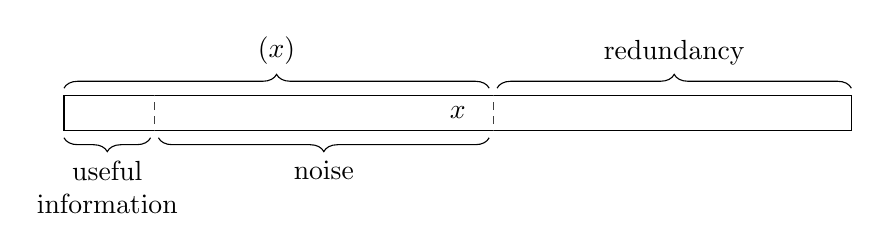
\begin{tikzpicture}[decoration={brace,amplitude=5pt}]
    \draw (0, 0) rectangle (10, 3ex);
    \node at (5, 1.5ex) {$x$};
    \draw[decorate,yshift=2.5pt] (0, 3ex) -- (5.4, 3ex)
      node[midway,above=5pt] {$\KC(x)$};
    \draw[decorate,yshift=2.5pt] (5.5, 3ex) -- (10, 3ex)
      node[midway,above=5pt] {redundancy};
    \draw[decorate,yshift=-2.5pt] (5.4, 0) -- (1.2, 0)
      node[midway,below=5pt] {noise};
    \draw[decorate,yshift=-2.5pt] (1.1, 0) -- (0, 0)
      node[midway,below=5pt,align=center] {useful \\ information};
    \draw[densely dashed,dash phase=(4pt-1.5ex),darkgray]
      (1.15, 0) -- ++(0, 3ex)
      (5.45, 0) -- ++(0, 3ex);
  \end{tikzpicture}
  % 11% useful, 43% noise, 46% redundant, like in Example 3.4.2.
  \caption{
    The length of a string~$x$, decomposed into the Kolmogorov complexity of~$x$ and the redundancy in~$x$.
    The Kolmogorov complexity is further decomposed into useful information and useless noise.
    Relative sizes are depicted in accordance with Example~\ref{ex:bmp_png_jpeg}.
  }
  \label{fig:length_decomposed}
\end{figure}

That not all of some object's natural length is allotted to useful information can also be seen from information-hiding techniques.
Homoglyphs are text characters that are not perceived to be different, yet have different encodings.
By selectively replacing characters in a text message by their homoglyphs, information can be injected into a message without ostensibly altering it.
Arguably, the information in a text message is not even altered when words or phrases in it are replaced by synonyms.
This, too, can be used for information hiding, or, more technically, for \defkey{steganography}~\parencite{hosmani2015dual}.

While the useful information is left unaltered by steganography, this does not mean that the presence of hidden information cannot be detected.
Such detection is the goal of \emph{steganalysis}.
For instance, it is not unreasonable to expect that the use of homoglyphs reduces the redundancy in a message.
Thus, a carrier message \emph{without} hidden information may be more compressible than a message \emph{with} hidden information.
Applied to images, techniques are developed to restrict the action of steganographic information hiding to the noise in an image.
These techniques evade detection by simple compression tests.
An overview of steganography methods for images is given by \textcite{cheddad2010digital}.

\subsubsection{Synopsis}
Quantifying the useful information in an object is the domain of \emph{algorithmic statistics}.
This is a formulation of statistics centered on model selection for individual data samples.
Algorithmic statistics will be introduced in more detail in Section~\ref{sec:statistics:algorithmic}.
The associated formalization of useful information, \emph{sophistication}, is the topic of Section~\ref{sec:statistics:sophistication}.
Algorithmic statistics includes a notion of goodness-of-fit grounded in Kolmogorov complexity, where computational resource usage is not considered.
Consequently, sophistication targets a universal observer with unbounded computational powers.
This approach is complicated by the fact that, unlike Kolmogorov complexity, sophistication differs in an unbounded way among universal observers.
That is, sophistication is sensitive to the encoding used for specifying procedures.
Additionally, if we consider reasoning to be a form of computation, then it makes sense to include computational complexity in a measure of useful information.
This should make it possible to target a human observer instead of a universal observer.
With parameterizations, we can formalize useful information in a context-sensitive way.
Moreover, since parameter values can provide a measure of computational complexity, a parameterized sophistication can include computational considerations.
Doing so tightens the relationship between algorithmic complexity and computational complexity.

Previously, we looked at the relationship between parameter values and the algorithmic complexity of individual strings.
Here, we shall continue that investigation.
We shall see that parameterizations provide an alternative to the use of Kolmogorov complexity in algorithmic statistics.
The parameterized take on algorithmic statistics includes the traditional version as a special case.
This enables us to use traditional algorithmic statistics as a running example in the section on sophistication, Section~\ref{sec:statistics:sophistication}.

Many theorems and questions that are central to algorithmic statistics are about the existence and prevalence of objects that lack simple statistical models.
In Section~\ref{sec:statistics:stochasticity}, we continue our generalization of algorithmic statistics so that parameterized counterparts to such theorems and questions can be stated.
We observe that the idea of simplicity of a model for an object requires a notion of length to be available for the object.
Throughout our treatment of parameterized algorithmic statistics, we make a distinction between an object and a string representation of that object.
Therefore, a notion of length is only available for objects after we have decided on a way to encode objects.
This lets us conclude that an \emph{object} can only be incompressible if it has a truly canonical encoding, which is only the case if the object is already a string.

In Section~\ref{sec:statistics:estimation}, we get to see how the inclusion of parameterizations makes the theory of algorithmic statistics more fine-grained.
The section places sophistication in the context of three well-known strategies for model selection in statistics: Occam's razor, the maximum likelihood principle, and the minimum description length principle.
Additionally, in this section we find that most strings have simple models, also in parameterized algorithmic statistics.
These simple models would even pass as good simple models in traditional algorithmic statistics for infinitely many objects.
Thus, for infinitely many objects, the useful information reflected by a parameterization is really all the useful information there is.

Questions surrounding the prevalence of objects with simple models can also be turned around in parameterized algorithmic statistics.
We do so in Section~\ref{sec:statistics:encodings_distributions}, where we focus on parameterizations corresponding to parameterized algorithms that are successfully applied in practice.
From the success of these algorithms, we can infer what parameter values we are most likely to encounter.
To wit, we know that the expected parameter value is small, like we have seen all the way back in Example~\ref{ex:type_inference}.
For a fixed parameterization, this gives us information about what a good statistical model of the real world should look like.
In turn, this knowledge can be used as a guiding principle in the design of suitable data structures for dealing with real-world data.
Section~\ref{sec:statistics:data_structures} explores the properties and possibilities of data structures rooted in parameterizations.

\subsection{An Overview of Algorithmic Statistics}
\label{sec:statistics:algorithmic}\indexkey{algorithmic statistics}%
The crucial insight that makes algorithmic statistics possible is that the Kolmogorov complexity of an object can always be realized by a two-part code.
Every object can be described by two strings of which the combined length equals, up to an independent additive constant, the Kolmogorov complexity of the object.
The two parts are commonly called \defkey{model} and \defkey{data-to-model code}.
The second part is so named because it describes the object relative to the model.
In the pairing of the two parts it must be clear where one part ends and the other begins.

In traditional applications of the minimum description length principle~\parencite{rissanen1978modeling,rissanen1983universal,vitanyi2000minimum,grunwald2007minimum} the word `model' is used to indicate a functional form.
The second part of the two-part code is then used to both instantiate a single function \emph{and} specify the data with respect to it.
In algorithmic statistics, however, the two-part code should separate the meaningful information in an object from the random noise in that object.
Algorithmic statistics is not concerned with any structure inside the second part of the two-part code.
Thus, the word `model' is used for what is known as a \emph{point hypothesis} or \emph{exact hypothesis} in inferential statistics.
More concretely, in algorithmic statistics, we interpret models as probability distributions.
In turn, data-to-model codes are interpreted as entropy encodings in accordance with those probability distributions~\parencite{vereshchagin2004kolmogorov,cover2006elements}.

A measure of the informativeness, the \defkey{sophistication}, of an object is available in the form of the minimum complexity of a model for the object.
This minimization is restricted to those probability distributions with which the two-part code for the object realizes the Kolmogorov complexity of the object.
Unfortunately, there is no clear-cut way to define the complexity of a probability distribution.
If we would allow the universal distribution~\parencite{li2008introduction} to have a finite complexity, then it would realize the Kolmogorov complexity of every object.
The finite complexity of the universal distribution would present a constant additive overhead to the Kolmogorov complexity.
However, Kolmogorov complexity is only defined up to an additive constant.
Likewise, the universal distribution is only defined up to a multiplicative constant.
Hence, this additive overhead is unavoidable to begin with.
In that sense, the universal distribution would act as a universal model~\parencite{vitanyi2006meaningful,bloem2015two}.
Disregarding additive constants for a moment, we see that such a universal model would place a universal bound on the informativeness of any object.
This renders our measure of informativeness useless.
To which probability distributions we assign finite complexity is hence a central question in the development of algorithmic statistics~\parencite{vereshchagin2017algorithmic}.
The class of probability distributions considered is called the \emph{model class}.
While the choice of a model class is usually an ad~hoc choice in applications of the minimum description length principle~\parencite{vitanyi2000minimum,grunwald2007minimum}, algorithmic statistics calls for a single generic model class.
The lack of a universally best model class, according to some motivation from outside the theory, is a major obstacle for algorithmic statistics.

Many model classes have been considered in the existing literature.
When interpreted as classes of probability distributions, there is significant variation in the requirements that have been put on the computability of the probabilities.
Regardless of this variation, the studied model classes can be characterized by a classification of the \emph{support} of the probability distributions they contain.
Least restrictive are the model classes where the support of a probability distribution can be any semidecidable set.
Such model classes are present in the works of \textcite{rissanen1983universal}, \textcite{koppel1988structure}, \textcite{gacs2001algorithmic} (as implicit probabilistic models), \textcite{vitanyi2006meaningful}, and \textcite{antunes2009sophistication}.
A model class where exactly the decidable sets occur as the support of the probability distributions is hinted at by \textcite{gacs2001algorithmic} (as explicit probabilistic models).
However, their definitions are not strong enough to enforce decidability.
The most fruitful model class has been that of uniform probability distributions with arbitrary, yet necessarily finite, support.
This is the model class originally proposed by Kolmogorov and most prominent in the works of \textcite{gacs2001algorithmic,vereshchagin2004kolmogorov}.
A slightly more general model class where the probability distributions have finite support, yet are allowed to take on different rational-valued probabilities on their support, was considered by \textcite{vereshchagin2017algorithmic}.

All of the model classes studied by the aforementioned authors exclude universal models.
Yet, none are presented with a guarantee against putting meaningful information in the data-to-model code, thus \emph{underfitting} the data.
As argued by \textcite{bloem2015two}, it is likely that these model classes do in fact contain models that are \enquote{too universal}.
That is, some models are universal enough to bound the informativeness of some objects by a value less than the informativeness we ascribe to them intuitively.
Such model classes misrepresent the informativeness of certain objects that we think of as containing meaningful information.
At the same time, \textcite{vereshchagin2009algorithmic,bloem2015two,antunes2017sophistication} show that the choice of the complexity measure used to measure the complexity of models matters.
Sophistication, which is described in more detail in the next section, in particular is sensitive to this choice.
While Kolmogorov complexity is invariant under the choice of a universal machine, sophistication, despite being based on Kolmogorov complexity, is not.
This is true regardless of how we adapt Kolmogorov complexity for measuring the complexity of probability distributions, which can be done in many ways~\parencite{gacs2001algorithmic}.
Slight variations in the model complexity can change a model from realizing the Kolmogorov complexity of an object to not realizing it and vice versa.
Hence the minimum complexity of a probability distribution with which the two-part description of an object realizes the Kolmogorov complexity of that object can change significantly with a change of the reference universal machine.
As a result, some choices of a reference machine may lead to widespread \emph{overfitting}~\parencite{bloem2015two}.
When performing maximum likelihood estimation, this form of overfitting can be mitigated by working with complexity-constrained subclasses of the model class~\parencite{vereshchagin2004kolmogorov}.
However, that brings us no closer to a definitive measure of the useful information in an object.
Alternatively, one can adjust the complexity measure for models so that the selection of overfitting models is penalized.
This is done by \textcite{rissanen1983universal,antunes2009sophistication}, but it is not proven to be adequate and may lead to underfitting instead~\parencite{bloem2015two}.

We propose to include the model class and its associated complexity measure as a degree of freedom in the framework of algorithmic statistics.
Indeed, we shall use parameterizations as model classes with an inherent complexity measure.
Besides addressing underfitting and overfitting, doing so also makes it possible to examine complexity measures other than the Kolmogorov complexity.
The uncomputability of Kolmogorov complexity has been identified as an impediment to applications of algorithmic statistics~\parencite{rissanen1983universal,vereshchagin2017algorithmic}.
Remarkably, the existing literature on algorithmic statistics has so far only explored in detail variations of Kolmogorov complexity as complexity measures.
At the same time, the potential for restricted model classes has been identified~\parencite{bloem2014safe,vereshchagin2017algorithmic}.
By introducing an explicit dependence on a model class, we accept that a notion of useful information may be subject to one's expectations.
There appears to be no universally best model class, or, in other words, no universal prior for algorithmic statistics.
Because of that, the dependence of a notion of useful information on a model class is likely unavoidable.
\slogan[\label{slo:useful_information}]{Useful information is context-dependent.}
Accepting that a notion of useful information is dependent on a model class justifies the addition of a model class variable to the framework.

\subsection{Sophistication}
\label{sec:statistics:sophistication}%
Traditionally, algorithmic statistics looks at describing a string~$x$ with the help of a probability distribution~$P$ that assigns nonzero probability to~$x$.
The probability mass function~$P$ is required, at the least, to be rational-valued and computable~\parencite{vereshchagin2017algorithmic}.
Knowing~$P$, a code that is optimal with respect to~$P$ uses $-\log P(x)$~bits for describing~$x$ in prefix-free fashion~\parencite{cover2006elements}.
Now, let us use $\length{P}$ for the length of a description of~$P$ in some fixed prefix-free encoding of rational-valued computable probability mass functions.
We find an upper bound on the Kolmogorov complexity of~$x$ in the form of a two-part description of~$x$,
\begin{equation*}
  \KC(x) \le \length{P} - \log P(x).
\end{equation*}
How tight this bound can get depends on the chosen method of encoding probability mass functions.
It is customary to focus on methods that are as efficient as possible.
An extreme case is provided by the probability distributions~$P$ of which the support is a singleton,~$\{x\}$, and we have $P(x) = 1$.
For such a probability distribution~$P$, the length $\length{P}$ can be made to match, up to an additive constant, the Kolmogorov complexity of~$x$.
With encodings that accomplish this, the above equation can become an equality.

Since we are describing the string~$x$ using two-part codes, we may investigate the many ways in which a description of~$x$ can be composed of two parts.
In particular, we are interested in the ways the Kolmogorov complexity of~$x$ can be split in two by probability mass functions.
Naturally, when we restrict our model class, we limit the number of ways to describe~$x$.
However, some model classes nearly cover all possible ways to balance the lengths of the two parts.
One such model class is that of \emph{uniform} distributions.
The support of a uniform probability mass function is a finite set.
For a finite set~$A$, let $\langle A\rangle$ denote a listing of all elements of~$A$ and notice that the number of elements of~$A$ can be recovered from~$\langle A\rangle$.
\begin{theorem}[{\textcite[Remark~1 \& Proposition~6]{vereshchagin2017algorithmic}}]\hspace{0pt}\\*
\label{thm:uniformmodels}%
  Let $P$ be a rational-valued computable probability mass function and $x$ a string to which $P$ assigns nonzero probability.
  There exists a finite set~$A$ of~$m$ elements including~$x$ such that we have
  \begin{equation*}
    \KC(\langle A\rangle) \le \length{P} + \bigO(\log \length{x}) \quad\text{and}\quad -\log \frac{1}{m} \le -\log P(x) + \bigO(1).
  \end{equation*}
\end{theorem}
In other words, up to terms logarithmic in the length of a string~$x$, we may restrict our attention to uniform distributions.
Uniform distributions effectively maximize the minimum probability in a distribution with a given finite support.
For distributions with a given infinite support, there is no clear-cut way of maximizing the minimum probability.
Therefore, it is interesting to note that there is a variant of Theorem~\ref{thm:uniformmodels} for a model class where distributions have potentially infinite support.
Note that the $-\log \frac{1}{m}$ term in Theorem~\ref{thm:uniformmodels} represents the fact that $\log m$ bits suffice to tell the elements of the finite set~$A$ apart.
With Elias~delta coding\indexkey{Elias~delta coding} as defined in Section~\ref{sec:preliminaries:binary}, we can single out the $r$th element of any decidable set using $\log r + 2 \log \log r$ bits.
Prefix-free codes such as the Elias~delta coding are related to probability distributions by the \defkey{Kraft~inequality}~\parencite{cover2006elements,li2008introduction}.
An element that is encoded using $\ell$~bits is accordingly assigned a probability of $2^{-\ell}$.
The probability distributions stemming from Elias~delta coding via the Kraft~inequality can have infinite support.
It is the model class of such distributions that has a property similar to that codified in Theorem~\ref{thm:uniformmodels} for the model class of uniform distributions.
For a decidable set~$A$, let $\KC(A)$ denote the least length among the lengths of decision procedures for~$A$.
\begin{theorem}
\label{thm:rankmodels}%
  Let $P$ be a rational-valued computable probability mass function and $x$ a string to which $P$ assigns nonzero probability.
  There exists a decidable set~$A$ including~$x$ such that, with $r \deq \rank(x : A)$, we have
  \begin{align*}
    \KC(A) &\le \length{P} + \bigO(\log \length{x})
  \shortintertext{and}
    \log r + 2 \log \log r &\le -\log P(x) + \bigO(1).
  \end{align*}
\end{theorem}
\begin{proof}
  Let $S$ be the support of~$P$ and let $r_S$ be the rank of~$x$ in this set.
  In other words, we define~$S$ as $\{y \st P(y) > 0\}$ and we define $r_S$ as $\rank(x : S)$.
  Furthermore, set~$i$ to the unique value for which we have
  \begin{equation*}
    \frac{i^2\, 2^i}{(\log r_S)^2\, r_S} < P(x) \le \frac{(i + 1)^2\, 2^{i + 1}}{(\log r_S)^2\, r_S}.
  \end{equation*}
  Observe that $i$ must be less than $\log r_S$, because $P(x)$ is at most~$1$.
  Therefore, we have $i \in \bigO(\length{x})$ and the number of bits needed to specify~$i$ is in $\bigO(\log \length{x})$.

  Now, consider the set
  \begin{equation*}
    H \deq \left\{y \st[\middle] P(y) > \frac{i^2\, 2^i}{(\log \rank(y : S))^2\, \rank(y : S)}\right\}.
  \end{equation*}
  We find that $x$ is included in~$H$.
  Observe that all members of~$H$ preceding~$x$ must have a probability of at least
  \begin{equation*}
    \frac{i^2\, 2^i}{(\log r_S)^2\, r_S}.
  \end{equation*}
  Therefore the rank of~$x$ in~$H$ is at most
  \begin{equation}
  \label{eq:rankmodels:rank}
    \frac{(\log r_S)^2\, r_S}{i^2\, 2^i},
  \end{equation}
  as otherwise the sum of the probabilities would exceed~$1$.
  The rank of~$x$ in~$H$ can thus be upper bounded by $\frac{1}{P(x)}$, which means $H$ almost satisfies the requirements on the set~$A$ of the theorem.
  To complete the proof, all that remains is to move some complexity from the data-to-model code into the model.
  The set~$H$ can be partitioned into $\length{x}^2$ subsets $H_1, H_2, H_3, \ldots, H_{\length{x}^2}$ via
  \begin{equation*}
    H_j \deq \{y \in H \st \rank(y : H) \equiv j \pmod{\length{x}^2}\}.
  \end{equation*}
  For exactly one~$j$, the set $H_j$ contains~$x$.
  Let $A$ be this set $H_j$.
  That is, $A$ is a thinned-out version of~$H$ that includes~$x$.
  By construction, $A$ contains at most one out of every $\length{x}^2$ elements of~$H$.
  Following \eqref{eq:rankmodels:rank}, the rank of~$x$ in~$A$ is therefore at most
  \begin{equation*}
    \frac{(\log r_S)^2\, r_S}{i^2\, 2^i} / \length{x}^2,
  \end{equation*}
  rounded upward if needed.
  Hence, the rank of~$x$ in~$A$ is at most $\frac{r_S}{i^2\, 2^i} + 1$ and if we let $r$ denote this rank, we find
  \begin{align*}
    \log r + 2 \log \log r &\le \log \frac{r_S}{i^2\, 2^i} + 2 \log \log \frac{r_S}{i^2\, 2^i} + \bigO(1) \\
    	&\le \log r_S - 2 \log i - i + 2 \log \log r_S + \bigO(1) \\
    	&\le -\log \frac{(i + 1)^2\, 2^{i + 1}}{(\log r_S)^2\, r_S} + \bigO(1) \\
    	&\le -\log P(x) + \bigO(1),
  \end{align*}
  as desired.
  Additionally, $A$ was constructed from $P$, $i$, and $j$, so we also have $\KC(A) \le \length{P} + \bigO(\log \length{x})$.
\end{proof}

The message of Theorem~\ref{thm:rankmodels} is that, up to terms logarithmic in the length of a string~$x$, we may restrict our attention to distributions in accordance with Elias~delta coding.\indexkey{Elias~delta coding}
This allows us to focus on decidable sets as models, and on parameterizations with decidable slices as model classes.
\begin{definition}
  A \defkeyat{parameterized!model}{parameterized model} is a slice of a parameterization, represented by its corresponding parameter value.
\end{definition}

We call a parameterization~$\eta$ a \defkeyat{parameterized!model class}{parameterized model class}, and a parameter value~$k$ an \emph{$\eta$"~model} for a string~$x$ if we have $x \in \eta_k$.\indexkey{model}
By using the same coding method across all slices, across all parameterizations even, we are able to isolate the useful information about an object.
We are unable to express any properties other than the rank of a string~$x$ in a slice~$\eta_k$ if our data-to-model code is confined to Elias~delta coding.
Therefore, useful information can only accumulate in a specification of the model, thus in the parameter value~$k$.

One way to think of a parameterization in this context is as a sort of alternative computability universe.
In such an alternative universe, the slices of the parameterization take the role of \enquote{decidable} sets.
Parameter values then encode the equivalent of the corresponding decision procedures.
Of course, when not all slices of the parameterization are decidable, this alternative universe is different from the universe we inhabit.
However, even when all slices are decidable, the parameterization may still challenge our notion of how computability behaves.
The parameter value associated with a slice may not be related to anything we would reasonably want to call a decision procedure for the slice.
On the other hand, when we can effectively map the parameter values to decision procedures for the respective slices, we are in a fairly restricted setting.
\begin{example}
\label{ex:decision_parameterization}%
  When we think of ways to encode procedures, we normally only think of so-called \emph{acceptable} encodings~\parencite{rogers1967theory}.
  Loosely speaking, there must be an effective way to interpret an encoded procedure and perform the computations it represents.
  All acceptable encodings lead to the same notion of Kolmogorov complexity.
  Our choice of an encoding has been somewhat implicit, but it plays a role in the parameterization given by
  \begin{equation}
  \label{eq:decision_parameterization}
    (\{x \st \text{$k$ encodes a decision procedure that accepts $x$}\})_{k \in \binary^+}.
  \end{equation}
  In this parameterization, there are two kinds of slices.
  For a parameter value~$k$ that encodes a decision procedure, the corresponding slice is the set decided by that decision procedure.
  In other words, the decision procedure encoded by~$k$ outputs~\bits{1} on the members of slice~$k$ and it outputs~\bits{0} on the nonmembers.
  However, if $k$ does not encode a decision procedure, for instance because $k$ does not encode a total function, then the corresponding slice is empty.
  Unfortunately, by Rice's theorem~\parencite{rice1953classes}, this means we cannot effectively map a parameter value to a decision procedure for the corresponding slice.
\end{example}

Suppose it is possible to map parameter values to decision procedures for the corresponding slices of a parameterization effectively.
Then, the minimum length of a decision procedure for a slice is, up to an additive constant, bounded from above by the length of the corresponding parameter value.
The additive constant only depends on the algorithmic complexity of the function mapping parameter values to decision procedures.
Because this constant is fixed for the parameterization, we may ignore it and use the length of a parameter value as the length of a decision procedure.
For more unusual parameterizations such a constant may not exist.
Yet, we may still use the length of a parameter value as a measure of the complexity of a slice.
In general, a nice starting point for measuring the algorithmic complexity of a string with respect to a parameterization is the following.
\begin{definition}
\label{def:pc}%
  The \defkeyat{parameterized!complexity}{parameterized complexity} of a string~$x$ with respect to a parameterization~$\eta$ is
  \begin{equation*}
    \pc_\eta(x) \deq \min\{\length{\pair{k}{\rank(x : \eta_k)}} \st k \in \binary^+\text{ such that we have $x \in \eta_k$}\}.
  \end{equation*}
\end{definition}

Note that, strictly speaking, the above definition should look at pairs of a parameter value and a \emph{string representation} of the rank.
To improve readability, we shall not explicitly state the conversion of the rank, which is a number, to a string when dealing with such pairs.

As parameterizations are covers of $\binary^+$, the parameterized complexity with respect to a parameterization is defined for every string.
The choice of a pairing function may have an effect on the parameterized complexity.
It may affect not only its value, but also the parameter value with which this value, as a minimum of multiple candidates, is realized.

\begin{example}[continued from Example~\ref{ex:decision_parameterization}]
\label{ex:traditional_pc}%
  Our pairing function, Definition~\ref{def:pairing_function}, uses a prefix-free code, the Elias~delta code, for its second component.
  As a result, the number of bits used to encode the rank in the definition of parameterized complexity aligns nicely with Theorem~\ref{thm:rankmodels}.
  The pairing function does not use a prefix-free code for its first component.
  However, when encoding procedures, it is natural to use a prefix-free code to begin with~\parencite{li2008introduction}.
  Suppose we use a prefix-free encoding of decision procedures in the parameterization given by~\eqref{eq:decision_parameterization}.
  In that case, parameterized complexity with respect to the parameterization given by~\eqref{eq:decision_parameterization} is essentially Kolmogorov complexity.

  To see that it is at most the Kolmogorov complexity, observe that for every string~$x$, there is a set~$\{x\}$ with a decision procedure of length $\KC(x) + \bigO(1)$.
  In the set~$\{x\}$, the rank of~$x$ is~$1$, hence the parameterized complexity of~$x$ is at most $\KC(x) + \bigO(1)$.
  At the same time, the Kolmogorov complexity of~$x$ cannot be substantially higher than its parameterized complexity.
  Consider a procedure that, given a string~$k$ and a number~$r$, simulates the decision procedure encoded by~$k$ and finds the~$r$th string accepted by it.
  This procedure recovers~$x$ from any~$\pair{k}{\rank(x : \eta_k)}$, whenever~$x$ is a member of~$\eta_k$.
  When we hardcode the pair $\pair{k}{\rank(x : \eta_k)}$, we obtain a new procedure of which the length is $\length{\pair{k}{\rank(x : \eta_k)}} + \bigO(1)$.
  Hence the parameterized complexity of~$x$ is not only at most $\KC(x) + \bigO(1)$, but also at least $\KC(x) - \bigO(1)$.
\end{example}

The example above demonstrates how parameterized complexity generalizes Kolmogorov complexity.
It showed that for some parameterization, the two notions of complexity coincide on all strings, up to an independent additive constant.
Other parameterizations may show the same behavior, or show it only for some strings.
We say that a parameterization~$\eta$ \defkeyat{Kolmogorov complexity!captured}{captures} the (Kolmogorov) complexity of a string~$x$ if, up to a fixed additive constant independent of $x$, we have $\pc_\eta(x) = \KC(x)$.
Note that in this definition, several hidden constants are at work.
To be precise, we should first choose a constant~$c$ and fix a reference encoding of procedures that we use to define Kolmogorov complexity.
Having done so, a parameterization~$\eta$ captures the complexity of those strings~$x$ for which we have
\begin{equation*}
  \KC(x) - c \le \pc_\eta(x) \le \KC(x) + c.
\end{equation*}

One benefit of parameterized complexity over Kolmogorov complexity is that it can be computable, even if it captures the complexity of some strings.
\begin{lemma}
\label{lem:pccomputable}%
  If $\eta$ is a decidable parameterization, then $\pc_\eta$ is a computable function.
\end{lemma}
\begin{proof}
  A procedure computing the parameterized complexity of a string~$x$ could proceed as follows.
  \begin{codelisting}
  \item
    \code{For each} parameter value~$k$, in order of increasing length:
    \begin{codelisting}
    \item
      \code{If} $\eta_k$ includes~$x$,
      \itemcont \code{break} out of the current loop and continue at step~\ref{code:pc:bounded}.
    \end{codelisting}
  \item\label{code:pc:bounded}%
    \code{For each} parameter value~$k'$ of length at most $\length{\pair{k}{\rank(x : \eta_k)}}$:
    \begin{codelisting}
    \item
      \code{If} $\eta_{k'}$ includes~$x$ and $\length{\pair{k'}{\rank(x : \eta_{k'})}}$ is less than $\length{\pair{k}{\rank(x : \eta_k)}}$,
      \itemcont \code{set} $k$ to~$k'$.
    \end{codelisting}
    \item
      \code{Return} $\length{\pair{k}{\rank(x : \eta_k)}}$.
  \end{codelisting}
  The unbounded loop at the first step of this algorithm is guaranteed to be exited from, because $\eta$ is a cover of $\binary^+$.
  The bounded loop at the second step makes sure that the returned value is indeed the minimum length of all candidate lengths.
  Thus, the returned length is the parameterized complexity of~$x$ with respect to~$\eta$.
  Note that the algorithm is allowed to test whether a slice of~$\eta$ includes~$x$ because $\eta$ is assumed to be decidable.
\end{proof}

For a given string~$x$, there may be more than one parameterized model that witnesses the minimum in the definition of parameterized complexity.
Those that do are particularly interesting parameterized models of~$x$.
Because they realize the parameterized complexity of~$x$, these models contain all information about~$x$ that is available in the parameterization.
This is a form of \emph{sufficiency}, as used in parametric probabilistic statistics \parencite[see also][Section~2.9]{cover2006elements}.
\begin{definition}
  A parameter value~$k$, with respect to a parameterization~$\eta$, constitutes a \defkeyat{parameterized!sufficient statistic}{sufficient parameterized statistic} for a string $x \in \eta_k$ if we have
  \begin{equation*}
    \length{\pair{k}{\rank(x : \eta_k)}} = \pc_\eta(x).
  \end{equation*}
  In other words, an $\eta$"~model~$k$ for~$x$ is a sufficient parameterized statistic if $\length{\pair{k}{\rank(x: \eta_k)}}$ is minimal.
\end{definition}

\begin{example}
  In parametric probabilistic statistics, we are dealing with model classes indexed by a parameter, say, $\theta$.
  A \emph{statistic} is a function of a data sample into some arbitrary set and it is \emph{sufficient} if it preserves the information in the sample about the parameter.
  The identity function is always a sufficient statistic, but more interesting sufficient statistics may be available.
  The textbook example is a binomial distribution with a fixed number of trials,~$n$, and an unknown success probability for each trial,~$p$.
  The model class is then the class of binomial distributions with parameters $n$ and~$p$.
  As $n$ is fixed, this class is indexed by~$p$.

  Given a data sample of the outcomes of~$n$ trials, we can make a prediction about the value of~$p$ that was used in generating the sample.
  The only property of the sample that is relevant for our judgment turns out to be the number of successes.
  If there are $i$ successes in our sample, our best guess for the parameter~$p$ is $\frac{i}{n}$.
  Indeed, the mapping from the sample to the number of successes is a sufficient statistic.

  The relation to our parameterized sufficiency criterion is most visible with respect to the parameterization given by~\eqref{eq:decision_parameterization}.
  With that parameterization, a parameter value~$k$ that encodes a decision procedure for a set~$S$ is a sufficient statistic for a string~$x$ if we have
  \begin{equation*}
    \length{\pair{k}{\rank(x : S)}} = \KC(x).
  \end{equation*}
  The right side of this equation can be interpreted as \enquote{all the information in~$x$}.
  The equation thus states that when we replace~$x$ by its rank in~$S$, we have not lost any of the information in~$x$.
  In other words, $k$ preserves the information in~$x$ about decidable sets that contain~$x$.
  It is in this sense that a sufficient parameterized statistic is related to a sufficient probabilistic statistic.
\end{example}

Looking at the sufficient parameterized statistics for a string~$x$, we can see what complexity we should expect, at least, of a parameterized model for~$x$.
To use this minimum model complexity as a measure of the informativeness of~$x$ was suggested by~\textcite{koppel1988structure}.
Conceptually, however, it is a notion of simplicity needed for a formalization of Occam's razor.
While the razor has received lots of criticism, it has proven its worth many times, in both theory and applications~\parencite{grunwald2007minimum}.
\begin{definition}
  The \defkeyat{parameterized!sophistication}{parameterized sophistication} of a string~$x$ with respect to a parameterization~$\eta$ is
  \begin{equation*}
    \soph_\eta(x) \deq \min\{\length{k} \st \text{$k$ is a sufficient parameterized statistic for $x$}\}.
  \end{equation*}
\end{definition}

Notice that, for every parameterization~$\eta$ and string~$x$, the sophistication $\soph_\eta(x)$ is lower bounded by $\mu_\eta(x)$,
\begin{equation*}
  \mu_\eta(x) \le \soph_\eta(x).
\end{equation*}
Indeed, the parameterized sophistication~$\soph_\eta$ need not equal the minimization function~$\mu_\eta$.
For example, the minimization with respect to the parameterization given by~\eqref{eq:decision_parameterization} is bounded from above by the length of a decision procedure for~$\binary^+$.
However, the sophistication with respect to that parameterization can get arbitrarily large.
Still, when $\eta$ satisfies
\begin{equation}
\label{eq:compatible_strong}
  \forall k, k'\colon \length{k} \le \length{k'} \implies \eta_k \subseteq \eta_{k'},
\end{equation}
the rank of a string in a slice only increases with the length of its $\eta$"~models.
In other words, when the inclusion order of~$\eta$ is compatible with the encoding of the parameter, a stronger version of~\eqref{eq:compatible}, the functions $\soph_\eta$ and $\mu_\eta$ \emph{do} coincide.\indexkey{parameter!encoding!compatible with inclusion order}
Note that when~$\eta$ is decidable, $\soph_\eta$ is a computable function.
This result is similar to the computability of $\pc_\eta$ and can also be seen in the proof of Lemma~\ref{lem:pccomputable}.

\begin{example}[continued from Example~\ref{ex:traditional_pc}]
  The traditional notion of sophistication by \textcite{koppel1988structure} is essentially sophistication with respect to the parameterization given by~\eqref{eq:decision_parameterization}.
  Conceptually, sophistication is an algorithmic minimal sufficient statistic~\parencite{gacs2001algorithmic,vereshchagin2004kolmogorov}.
  The most common model class with respect to which sophistication is computed is the model class of finite sets~\parencite{bloem2015two}.
  Using Theorem~\ref{thm:uniformmodels}, it is then argued that, in effect, the entire class of rational-valued computable probability mass functions is taken into account.
  Similarly, our definition with respect to the parameterization given by~\eqref{eq:decision_parameterization} pertains to this broad class by Theorem~\ref{thm:rankmodels}.

  One thing to note is that traditional sophistication is defined with reference to a traditional notion of an algorithmic sufficient statistic.
  The benchmark for this traditional notion is Kolmogorov complexity, whereas the notion of a sufficient parameterized statistic hinges on parameterized complexity.
  The Kolmogorov complexity of a string depends on a chosen encoding of procedures, and is therefore only defined up to an additive constant.
  As a result, traditional sophistication is dependent on the choice of a constant.
  For parameterized sophistication, the choice of a constant is replaced by the choice of a parameterization.
\end{example}

\phantomsection\label{p:inference}%
Whatever parameterization~$\eta$ we are working with, each string~$x$ is assigned a finite sophistication $\soph_\eta(x)$.
This is a consequence of the fact that parameterizations are covers of~$\binary^+$.
In particular, for every parameterized model class~$\eta$ and every string~$x$, there is an $\eta$"~model for~$x$ that is a sufficient parameterized statistic for~$x$.
Thus, in a probability theory derived from~$\eta$, we are able to carry out statistical inference on samples of only a single object, the string~$x$.
In this probability theory, we can assign a prior probability to each slice of~$\eta$ as a function of the length of the corresponding parameter value.
For instance, we may do so by fixing a prefix-free encoding of parameter values and using the Kraft~inequality.\indexkey{Kraft~inequality}
This highlights a similarity between two-part codes and Bayesian statistical inference~\parencite{grunwald2007minimum}.
The probability of the event is then similarly assigned using the Kraft~inequality and the length of the rank in the slice, encoded in a prefix-free way.
Using our pairing function, Definition~\ref{def:pairing_function}, the parameterized complexity, Definition~\ref{def:pc} depends on an Elias~delta encoding of the rank.
We may use the same encoding for parameter values.
If we use $\ell(z)$ to denote the length of the Elias~delta encoding of the string~$z$, we can be a bit more precise about our probability distributions.
The prior probability of a slice corresponding to a parameter value~$k$ becomes~$2^{-\ell(k)}$.
Likewise, given an $\eta$"~model~$k$ for a string~$x$, the probability of~$x$ in this model becomes $2^{-\ell(\asStr(\rank(x : \eta_k)))}$.
These two probability distributions enable statistical inference.

Apart from being a cover of~$\binary^+$, parameterizations, as families of sets, are also directed.
Consequently, not only singleton samples are events, but all finite samples are events.
For every parameterized model class~$\eta$ and every finite set of strings~$X$, there is an $\eta$"~model~$k$ such that~$X$ is included in~$\eta_k$.
An investigation of algorithmic statistics in light of finite events of more than one string was carried out by \textcite{milovanov2016algorithmic}.
The model class used by \citeauthor{milovanov2016algorithmic} is that of finite sets.
To enable similar investigations in more general model classes, a few conditions to model classes are outlined by \textcite[Section~6.1]{vereshchagin2017algorithmic}.
By being directed, parameterizations meet their second condition, which requires that for every~$n$, some model must contain all strings of length~$n$.
This positions parameterizations as an alternative to the model classes of restricted type of \textcite{vereshchagin2017algorithmic}.
However, their model classes are also required to be decidable.
They place this requirement so that the emanating notions of complexity are bounded in one way or another by those derived from their most general model class.

\indexkey{sophistication}%
Let us denote the traditional sophistication, that with respect to the parameterization given by~\eqref{eq:decision_parameterization}, of a string~$x$ by $\soph(x)$.
Suppose $\eta$ is a decidable parameterization and denote by $\KC(\eta)$ the minimum length of a procedure that, given some $x$ and~$k$, decides whether $x$ is in $\eta_k$.
Then, we find, up to an additive constant,
\begin{equation}
\label{eq:soph}
  \soph(x) \le \soph_\eta(x) + \KC(\eta).
\end{equation}
This holds because every $\eta$"~model~$k$ for~$x$ has a Kolmogorov complexity bounded, up to an additive constant, by $\length{k} + \KC(\eta)$.
Even when~$\eta$ captures the complexity of~$x$, the above comparison of sophistications may be a strict inequality.
For example, the traditional sophistication of a string~$x$ of which the Kolmogorov complexity is roughly $\length{x} + 2 \cdot \log \length{x}$ is bounded from above by a constant.
This is because the set of all strings, $\binary^+$, is a sufficient model for such a string.
However, $\binary^+$ need not occur as a slice of~$\eta$, even when $\eta$ captures the complexity of~$x$.
Therefore, the parameterized sophistication of such strings need not be bounded by a constant and the two notions of sophistication can differ.

Outside of decidability requirements, similar parameterizations may lead to different measures of sophistication too.
As different ways of encoding decision procedures lead to different length measures, the length of a decision procedure is only defined up to an additive constant.
This additive constant is the bane of algorithmic statistics.
Surely, the various parameterizations defined by~\eqref{eq:decision_parameterization} for different encodings of decision procedures are all equivalent in the sense of Definition~\ref{def:uniform_order}.
However, as observed by \textcite{vereshchagin2009algorithmic,bloem2015two}, the universality of Kolmogorov complexity does not guarantee the invariance of sophistication up to an additive constant.
Which parameterized models count as sufficient parameterized statistics is sensitive to the chosen encoding of decision procedures.
Specifically, for technical reasons, the sufficiency criterion in traditional algorithmic statistics involves an additive slack-constant.
A change in the encoding of decision procedures can make some models sufficient statistics that were not sufficient statistics before, and vice versa.
Thus, the encoding of decision procedures affects the ensuing measure of sophistication.

\subsection{Stochasticity}
\label{sec:statistics:stochasticity}%
If a string~$x$ is random, then all bits of~$x$ contribute to the information in~$x$.
By a straightforward counting argument, we know that random strings exist~\parencite{li2008introduction}.
A related question that is not as easily answered, is whether or not strings exist of which all bits contribute to \emph{useful} information.
It was shown by \textcite{shen1983concept} that for each~$n$, there is a string of length~$n$ of which the traditional sophistication is at least $\frac{n}{2} - \bigO(\log n)$.
Later, \textcite{gacs2001algorithmic} improved this bound to $n - \bigO(\log n)$.
Thus, in traditional algorithmic statistics it is indeed possible for most of the $n$~bits to count toward useful information.
This is fairly surprising, because the traditional sophistication of a random string can be bounded from above by a constant.
For every random string, the set $\binary^+$ is a sufficient statistic with respect to the parameterization defined by~\eqref{eq:decision_parameterization}.

A difference between parameterized algorithmic statistics and the traditional form can be seen in the treatment of random strings.
While the traditional sophistication of a random string is very low, the parameterized sophistication with respect to an informative parameterization~$\eta$ is not.\indexkey{parameterization!informative}
This is a consequence of Theorem~\ref{thm:randomhard} and the fact that the minimization function~$\mu_\eta$ lower bounds the sophistication~$\soph_\eta$.
In other words, what is traditionally considered noise, may become information in the context of a parameterization.
We take this as further evidence supporting Slogan~\ref{slo:useful_information}: useful information is context-dependent.

That random strings may contain a substantial amount of useful information violates one of the original intuitions about what useful information is.
A common perception is that neither strings of minimum Kolmogorov complexity, nor strings of maximum Kolmogorov complexity can be rich in useful information~\parencite{adriaans2012facticity}.
Useful information, it is often thought, should strike a balance between these two extremes~\parencite{vitanyi2006meaningful,adriaans2012facticity}.
Challenging this intuition is the goal of lossy data compression, which is to extract from a string its useful information.
When the length of a string is divided into useful information, noise, and redundancy, as in Figure~\ref{fig:length_decomposed} on page~\pageref{fig:length_decomposed}, we observe that useful information is necessarily incompressible.
In that sense, useful information is random.
Therefore, the output of a lossy compression routine is ideally both high in useful information and high in Kolmogorov complexity.
Of course, lossy compression is specific to a certain domain, such as images.
Without knowing this domain, a compressed string may not appear particularly informative.
More generally, contrary to Kolmogorov complexity, a notion of length is wholly determined by the chosen method of encoding.
Since randomness revolves around a comparison between Kolmogorov complexity and length, randomness too is dependent on the chosen method of encoding.
This matters, because if there is any structure to the objects in a given domain, there is no longer a unique way of encoding those objects.
\slogan[\label{slo:random_object}]{There is no such thing as a random object unless the object is a string and nothing but a string.}

Sophistication focuses on sufficient statistics.
Sufficiency of a parameterized model is a robust concept and no hidden additive constants are involved.
Still, we may want to take parameterized models that are \emph{nearly} sufficient into account in our analysis of the information in a string.
For this, we measure how far away a parameterized model is from being a sufficient parameterized statistic~\parencite{vereshchagin2017algorithmic}.
\begin{definition}
\label{def:deficiency}%
  The \defkeyat{parameterized!optimality deficiency}{parameterized optimality deficiency} of a string~$x$ in a parameterized model~$k$ with respect to a parameterization~$\eta$ is
  \begin{equation*}
    \updelta_\eta(x, k) \deq \length{\pair{k}{\rank(x : \eta_k)}} - \pc_\eta(x).
  \end{equation*}
  When $k$ is not a parameterized model for~$x$, we set $\updelta_\eta(x, k) \deq \infty$.
\end{definition}

Note that, for every parameterized model~$k$, most strings in~$\eta_k$ have a parameterized optimality deficiency not much greater than~$\length{k}$.
More precisely, for all constants $n$ and~$c$, there are roughly $2^n$~strings~$x$ with $\length{\pair{k}{\rank(x : \eta_k)}} = \length{k} + n$, while there are at most $2^{n - c + 1}$ that satisfy $\pc_\eta(x) \le n - c$.
In other words, at most a $2^{-c + 1}$-fraction of strings satisfy $\updelta_\eta(x, k) \le \length{k} + c$.

Additionally, observe that the parameterized optimality deficiency of~$x$ is~$0$ precisely when $k$ is a sufficient parameterized statistic for~$x$.
On the basis of optimality deficiency, we can express whether a string has parameterized models of a given length that meet a required level of sufficiency.
\begin{definition}
  Let $\alpha$ and~$\beta$ be natural numbers and $\eta$ a parameterization.
  A string~$x$ is \defkeyat{parameterized!stochasticity@$(\alpha, \beta)$-stochasticity}{$(\alpha, \beta)$"~$\eta$"~stochastic} if there is an $\eta$"~model~$k$ for~$x$ satisfying
  \begin{equation*}
    \length{k} \le \alpha \quad\text{and}\quad \updelta_\eta(x, k) \le \beta.
  \end{equation*}
\end{definition}

The purpose of the numbers~$\alpha$ and~$\beta$ is perhaps best explained through an example.
\begin{example}
  \indexkey{example!1729}%
  The number \num{1729} enjoys some fame for being very much not a dull number.
  It is known as the \emph{Hardy--Ramanujan number}, after a visit from Godfrey~H.~Hardy to Srinivasa Ramanujan in which the number was discussed.
  At first, it may seem that the number does not have any striking features.
  It did so to Hardy, anyway.
  To make precise what this means, we need something like a parameterized model class~$\eta$ of number theoretic properties.
  We may expect that, when~$k_\text{odd}$ is the $\eta$"~model of odd numbers, the number \num{1729} is $(\length{k_\text{odd}}, \beta)$"~$\eta$"~stochastic for some small value of~$\beta$.
  That is, we may expect that there is not much more to \num{1729} than it being odd.
  However, \num{1729} is the \num{261}st product of three distinct primes.
  While we have not pinned down~$\eta$ exactly, we may expect that being the product of three distinct primes is a fairly simple property.
  As \num{1729} is only the \num{865}th odd number, the parameterized optimality deficiency of \num{1729} in~$k_\text{odd}$ may not be so small after all.
  Instead, we are better off modeling \num{1729} with the $\eta$"~model of products of three distinct primes, $k_{3\text{-primes}}$.
  Still, we may not have that \num{1729} is $(\length{k_{3\text{-primes}}}, \beta)$"~$\eta$"~stochastic for any too small value of~$\beta$.
  This is because \num{1729} is also the first number that is the sum of two cubes of positive numbers in two different ways.
  Thus \num{1729} is the first member of the model of numbers that are the sum of two cubes of positive numbers in multiple ways, $k_{2\text{-cubes}}$.
  While this last model is the most complex, it is quite likely that it determines the sophistication of \num{1729}.
  In summary, we have three $\eta$"~models for \num{1729}, satisfying
  \begin{gather*}
    \length{k_\text{odd}} \le \length{k_{3\text{-primes}}} \le \length{k_{2\text{-cubes}}}, \\
  \shortintertext{and}
    \updelta_\eta(\num{1729}, k_{2\text{-cubes}}) \le \updelta_\eta(\num{1729}, k_{3\text{-primes}}) \le \updelta_\eta(\num{1729}, k_\text{odd}).
  \end{gather*}
\end{example}

Traditionally, stochasticity is not defined using optimality deficiency, but using a slightly different deficiency measure known as \emph{randomness deficiency}~\parencite{shen1983concept,li2008introduction}.
These two deficiency measures can differ.
For traditional algorithmic statistics, \textcite[Theorem~2]{vereshchagin2017algorithmic} have shown that both measures lead to essentially the same notion of stochasticity.
The same holds true for restricted model classes, thanks to a result of \textcite{vereshchagin2010rate} \parencite[see also][]{vereshchagin2017algorithmic}.
Because it fits our framework better, we therefore prefer optimality deficiency over randomness deficiency.

Let us take a look at the stochasticity of a string~$x$ in relation to a parameterization~$\eta$.
There is a frontier of values of $\alpha$ and~$\beta$ beyond which $x$ is $(\alpha, \beta)$"~$\eta$"~stochastic~\parencite{vereshchagin2004kolmogorov,gacs2001algorithmic}.
Suppose that $\alpha$ and~$\beta$ are so that $x$ is $(\alpha, \beta)$"~$\eta$"~stochastic.
There is then an $\eta$"~model of complexity at most $\alpha$ that is within~$\beta$ of being a sufficient parameterized statistic for~$x$.
Sometimes, relaxing the sufficiency requirement slightly means that simple models become available.
Thus, a string~$x$ may be $(\alpha, \beta)$"~$\eta$"~stochastic for values of~$\alpha$ and~$\beta$ that are reasonably small in relation to its length $\length{x}$.
Such a string~$x$ is informally said to be \emph{stochastic}~\parencite{vereshchagin2017algorithmic}.
Indeed, a small value of~$\alpha$ reflects a high prior probability of the model in accordance with our discussion on page~\pageref{p:inference}.
Also, as noted following the definition of parameterized optimality deficiency, Definition~\ref{def:deficiency}, a small value of~$\beta$ suffices for most strings.

\begin{example}
  \indexkey{example!image compression}%
  In Example~\ref{ex:useful_information}, we encountered the JPEG lossy image compression format.
  The JPEG compression procedure contains a tuning parameter that determines the amount of degradation in quality that is considered admissible.
  This tuning parameter can range in value from $1$ to $100$, where $100$ represents near-perfect reproduction of the original image.
  Unfortunately, there is no unique minimal value of this parameter for which the degradation in image quality is unnoticeable to some reference observer.
  In other words, there is no clear-cut quality value beyond which a JPEG compressed image is a sufficient statistic for the original image.
  For Example~\ref{ex:useful_information}, a quality value of $90$ was used.

  With a lower quality setting, the JPEG compression procedure is able to produce smaller files.
  The compressed file size can be thought of as the size of a model for the original image.
  Thus, the $\alpha$~component of stochasticity acts like a bound on the file size.
  Because there is no proper sufficiency criterion for JPEG compression, the quality setting cannot directly be related to the $\beta$~component of stochasticity.
  However, there is a conceptual connection between lowering the quality setting and increasing the value of $\beta$.

  \begin{figure}
    \centering
    \begin{tikzpicture}
      \begin{axis}[
        width=10cm,
        no markers,
        xlabel={JPEG quality setting},
        ylabel={mean compressed file size (kilobytes)},
      ]
        \addplot table [y expr={\thisrowno{1}/1000}] {kodak.dat};
      \end{axis}
    \end{tikzpicture}
    \caption{
      The mean file size of the images in the Kodak True Color Image Suite~\parencite{franzen1999kodak} after JPEG compression at different quality settings.
    }
    \label{fig:jpeg_q}
  \end{figure}
  We are used to seeing a substantial decrease in file size when we allow the image quality to degrade only slightly.
  In Figure~\ref{fig:jpeg_q}, this can indeed be observed.
  At high values of the quality parameter, small changes have a large impact on the resulting file size.
\end{example}

The traditional notion of stochasticity is a special case of our parameterized one.
A string is called \emph{$(\alpha, \beta)$"~stochastic}, without mention of any~$\eta$, if it is stochastic in relation to the parameterization given~by~\eqref{eq:decision_parameterization}.
Not all strings are stochastic.
In fact, some of the strings of which the sophistication is close to the length are not stochastic at all.
Extending a similar result by \textcite{shen1983concept}, \textcite{gacs2001algorithmic} showed that some strings are only $(\alpha, \beta)$"~stochastic when $\alpha + \beta$ nearly exhausts the length of the string.
More specifically, for each~$n$, there is a string of length~$n$ that is only $(\alpha, \beta)$"~stochastic when $\alpha + \beta$ is at least $n - \bigO(\log n)$.
This result about the existence of \emph{non-stochastic} strings can be extended to the parameterized form of stochasticity.
If, given a parameterization~$\eta$, a string of length~$n$ is only $(\alpha, \beta)$"~$\eta$"~stochastic when $\alpha + \beta$ is at least $n - \bigO(\log n)$, then we say that the string is \emph{non-$\eta$"~stochastic}.
The following theorem relates the parameterized notion of stochasticity to the traditional one.
\begin{theorem}
\label{thm:stochastic}%
  Let $x$ be a string and $\eta$ a decidable parameterization.
  Denote by $\KC(\eta)$ the minimum length of a decision procedure for~$\eta$.
  Furthermore, define $\gamma \deq \pc_\eta(x) - \KC(x)$, meaning that $\eta$ captures the complexity of~$x$ if $\gamma$ is equal to~$0$.
  If $x$ is $(\alpha, \beta)$"~$\eta$"~stochastic, then it is $(\alpha + \KC(\eta), \beta + \gamma + \KC(\eta))$"~stochastic.
\end{theorem}
\begin{proof}
  Let $k$ be an $\eta$"~model for~$x$ witnessing that $x$ is $(\alpha, \beta)$"~$\eta$"~stochastic and let $j$ be the encoding of a decision procedure for~$\eta_k$ of minimum length.
  Recall from Example~\ref{ex:traditional_pc} that parameterized complexity in the traditional setting equals Kolmogorov complexity and observe that we have
  \begin{equation*}
    \length{j} \le \length{k} + \KC(\eta) \le \alpha + \KC(\eta).
  \end{equation*}
  It remains to show that the optimality deficiency of~$x$ in~$k$ with respect to~$\eta$ is at most $\beta + \gamma + \KC(\eta)$.
  The first step to this end follows the same reasoning as we have just encountered,
  \begin{align*}
    \updelta(x, j) &= \length{\pair{j}{\rank(x : \eta_k)}} - \KC(x) \\
    	&\le \length{\pair{k}{\rank(x : \eta_k)}} + \KC(\eta) - \KC(x)
  \intertext{which can then be expanded as}
    	&= \length{\pair{k}{\rank(x : \eta_k)}} + \KC(\eta) - \pc_\eta(x) + \gamma \\
    	&= \updelta_\eta(x, k) + \gamma + \KC(\eta) \\
    	&\le \beta + \gamma + \KC(\eta).
  \end{align*}
  Thus, $\eta_k$ witnesses that $x$ is $(\alpha + \KC(\eta), \beta + \gamma + \KC(\eta))$"~stochastic.
\end{proof}

When~$\eta$ is held fixed, $\KC(\eta)$ is constant and the theorem above can be seen as a translation from $\eta$"~stochasticity to traditional stochasticity.
The constant~$\gamma$ depends on~$x$ and only disappears when~$\eta$ captures the complexity of~$x$.
If the complexity of a non-stochastic string~$x$ is captured by a parameterization~$\eta$, then $x$ is also non-$\eta$"~stochastic.
This follows from the contrapositive formulation of Theorem~\ref{thm:stochastic}.
\begin{corollary}
\label{cor:nonstochastic}%
  Let $x$ be a string and $\eta$ a decidable parameterization.
  Furthermore, let $\gamma = \pc_\eta(x) - \KC(x)$ be the amount by which the complexity of~$x$ escapes~$\eta$.
  If $x$ is not $(\alpha, \beta)$"~stochastic, then it is not $(\alpha - \KC(\eta), \beta - \gamma - \KC(\eta))$"~$\eta$"~stochastic either.
\end{corollary}

The parameterization defined in~\eqref{eq:decision_parameterization} includes $\binary^+$ as a model.
Therefore, the minimization function with respect to that parameterization is bounded from above by a constant.
The same is not true of the sophistication.
Put differently, there is a constant~$\alpha$ such that for every string~$x$ there is a constant~$\beta_x$ such that $x$ is $(\alpha, \beta_x)$"~stochastic.
This constant,~$\beta_x$, cannot be bounded from above independently of~$x$.
The same cannot be said for stochasticity with respect to an arbitrary parameterization~$\eta$.
A string may fail to be $\eta$"~stochastic not only because simple $\eta$"~models are not good enough, but also because the string has no simple $\eta$"~models.
For all $\alpha < \mu_\eta(x)$, regardless of~$\beta$, the string~$x$ is not $(\alpha, \beta)$"~$\eta$"~stochastic.
The sophistication of~$x$ with respect to~$\eta$ may even be bigger than its length, $\soph_\eta(x) > \length{x}$.
For such~$x$ and~$\eta$, there are values of~$\beta$ with which~$x$ is not even $(\length{x}, \beta)$"~$\eta$"~stochastic.
Consequently, $\eta$ does not capture the complexity of~$x$ and the non"~$\eta$"~stochasticity of~$x$ is not a consequence of Corollary~\ref{cor:nonstochastic}.
Indeed, there would be no reason to assume that $x$ is non-stochastic in the traditional sense.

\subsection{Parameter Estimation}
\label{sec:statistics:estimation}%
In Lemma~\ref{lem:pccomputable}, we found that the parameterized complexity with respect to a decidable parameterization is computable.
Not only does this result extend to the computability of sophistication, it also entails that optimality deficiency is computable.
Therefore, for a fixed~$\alpha$ and~$\beta$, and a decidable~$\eta$, the set of $(\alpha, \beta)$"~$\eta$"~stochastic strings is decidable.
Moreover, for an $(\alpha, \beta)$"~$\eta$"~stochastic string~$x$, a witness,~$k$, of its stochasticity can be computed.
In particular, for the case where $\beta$ equals~$0$, we can compute an $\eta$"~model~$k$ for~$x$ such that we have $\length{k} = \soph_\eta(x)$.
Let us take a closer look at such mappings from a string~$x$ to an $\eta$"~model for~$x$.
As the $\eta$"~models are represented by parameter values, we can think of the model class conveyed by~$\eta$ as a model class indexed by parameter values.
In that sense, the model class conveyed by~$\eta$ is a parametric model class as known from probabilistic statistics.
Likewise, a mapping from strings to $\eta$"~models is also a mapping from strings to parameter values.
In other words, such a mapping is an \defkey{estimator}.
This probabilistic interpretation of concepts in algorithmic statistics has been recognized early on~\parencite{rissanen1983universal,vitanyi2000minimum,gacs2001algorithmic}.
An estimator that realizes the sophistication of its input is particularly exciting, as its output is a sufficient statistic that is as simple as can be.
While computable with respect to decidable parameterizations, the computation of such an estimator may be prohibitively resource intensive.
For this reason, alternative estimators are of interest.

So far, underlying our investigation has been a two-part code for describing a string~$x$.
If~$k$ is an $\eta$"~model for~$x$, then, knowing~$\eta$, we can recover~$x$ from
\begin{equation}
\label{eq:two-part}
  \pair{k}{\rank(x : \eta_k)}.
\end{equation}
We can minimize several quantities related to this two-part specification and each defines a different estimator.

The simplest model for~$x$ is one that minimizes the length of the first part of the specification, $\length{k}$.\indexkey{Occam's razor}
The corresponding~$k$ can be called the \defkeyat{estimator!Occam's razor}{Occam's razor} estimate, and its length equals~$\mu_\eta(x)$.
In traditional algorithmic statistics, this estimator is of no interest because the complexity of the simplest model for a string cannot exceed that of~$\binary^+$.
However, in parameterized algorithmic statistics, $\binary^+$ need not occur as a slice in any specific parameterization.

Rather than minimizing the length of the first part of the specification, we could also minimize the length of the second part, $\length{\rank(x : \eta_k)}$.
The corresponding $\eta$"~model~$k$ is one that contains as much information about~$x$ as possible, and is known as the \defkeyat{estimator!maximum likelihood}{maximum likelihood} estimate~\parencite{vereshchagin2004kolmogorov}.
In traditional algorithmic statistics, this estimator would yield a model, a finite set, of which the input string is the first element.
This is a form of overfitting, since all information about~$x$ now resides in the model part of the code, and none is left for the data-to-model part.
Again, in parameterized algorithmic statistics, a model like this need not occur as a slice in any given parameterization.

Minimizing the total length of the two-part specification of~$x$, we recover the \defkeyat{estimator!minimum description length}{minimum description length} estimator.\indexkey{minimum description length}
Equivalently, this estimator minimizes the sum of the lengths of both parts and as such balances the previous two estimators~\parencite{vereshchagin2004kolmogorov,rissanen1983universal}.
A parameter value obtained by this estimator, an estimate, is a sufficient statistic.
When we restrict to the simplest such models, we find that the length of a minimum description length estimate~$k$ is the sophistication~$\soph_\eta(x)$.

In summary, some natural estimators derived from the two-part description of a string, and their minimization objectives, are the following.
\begin{center}
  \begin{tabular}{r@{ }lcc}
    \multicolumn{2}{c}{\emph{estimator}}	& \emph{minimizes}	& \emph{length} \\
    \hline
    Occam's razor&(OR)	& first part	& $\mu_\eta$ \\
    maximum likelihood&(ML)	& second part	& \footnotesize{[no name]} \\
    minimum description length&(MDL)	& sum	& $\soph_\eta$
  \end{tabular}
\end{center}

The parameterization defined by~\eqref{eq:decision_parameterization} is not decidable and traditional algorithmic statistics pays attention to the computability of estimators.
One approach to the computability of estimators is to place an upper bound on the model complexity and consider each estimator as a function of this bound~\parencite{gacs2001algorithmic,vereshchagin2004kolmogorov} \parencite[in the presence of resource bounds,][]{milovanov2017algorithmic}.
Specifically, we consider ML and MDL relative to a selection of the slices of~\eqref{eq:decision_parameterization}.
The selection is obtained by including only those models of which the corresponding parameter value has a length shorter than the anticipated bound.
As mentioned before, OR is not interesting in the traditional context because it can be bounded from above by a constant.
On the other hand, ML and MDL are interesting, but, while the length of their estimates can be approximated from above, they are not computable~\parencite{vereshchagin2004kolmogorov}.
Of the two estimators, MDL is easier to approximate and therefore more convenient to work with in practice \parencite[Section~V.B]{vereshchagin2004kolmogorov}.
Additionally, as a function of a bound on the model complexity, MDL selects a sufficient statistic precisely when ML does \parencite[Lemma~IV.2]{vereshchagin2004kolmogorov}.
With respect to decidable parameterizations, OR, ML, and MDL would all be computable as a function of a bound on the length of parameter values.
Note, though, that without such a bound ML need not be computable.
Unfortunately, in the parameterized setting MDL cannot simply be used as a substitute for ML.
The tight correspondence between the two in traditional algorithmic statistics is not a given in the parameterized setting.

There are many more estimators than the three we have looked at so far, OR, ML, and MDL.
For a parameterization~$\eta$, we may look at those estimators that are in some sense consistent with~$\eta$.
\begin{definition}
  A function $\kappa\colon \binary^+ \to \binary^+$ is a \defkeyat{estimator!parameter estimator}{parameter estimator} for a parameterization~$\eta$ if it is consistent with~$\eta$ in the sense that, for all strings~$x$, we have $x \in \eta_{\kappa(x)}$
\end{definition}
\begin{example}
  Suppose $\kappa$ is a parameterization in the \citeauthor{flum2006parameterized} framework for parameterized complexity theory.
  On page~\pageref{eq:flum_parameterization}, we associated with this function the parameterization
  \begin{equation*}
    \eta \deq (\{x \st \asNat(\kappa(x)) \le \asNat(k)\})_{k \in \binary^+}.
  \end{equation*}
  For this parameterization, $\kappa$ is a polytime-computable parameter estimator.
\end{example}

We have seen that when~$\eta$ is decidable, the parameter estimators OR and MDL are computable.
Yet, even when $\eta$ is not decidable, a parameter estimator for~$\eta$ may be computable.
For instance, if $\kappa$ maps all strings to an encoding of a decision procedure for $\binary^+$, it is a computable parameter estimator for~\eqref{eq:decision_parameterization}.

\begin{example}[continued from Example~\ref{ex:p-cylinder}]
\label{ex:p-cylinder:estimator}%
  \indexkey{example!p-cylinder@\pdash{}cylinder}%
  Let $A$ be a \pdash{}cylinder and $g\colon \binary^+ \to \binary^+ \times \binary^+$ a corresponding isomorphism.
  Recall that we denote by~$g_1$ the first component of the image of~$g$ and that the parameterization based on~$g$ was defined as
  \begin{equation*}
    \eta \deq (\{x \st \asNat(g_1(x)) \le \asNat(k)\})_{k \in \binary^+}.
  \end{equation*}
  For this parameterization, $g_1$ is a parameter estimator.
  As $g_1$ is computable in polynomial time, it is also a parameterization in the sense of \citeauthor{flum2006parameterized}.
  Moreover, we have, for all~$x$,
  \begin{equation*}
    \mu_\eta(x) = \soph_\eta(x) = \length{g_1(x)}.
  \end{equation*}
  Note that~\eqref{eq:compatible_strong} holds for~$\eta$, so we find that OR, ML, MDL, and $g_1$ are all the same parameter estimator for~$\eta$.
\end{example}

As we have seen, a parameter estimator need not produce a sufficient parameterized statistic for its input.
However, we can get a pretty decent upper bound on the parameterized optimality deficiency of the estimates produced by a computable parameter estimator.
For this, we require two bounds involving the Kolmogorov complexity of a string~$x$.
The first of these is a straightforward extension of~\eqref{eq:soph} to parameterized complexity,
\begin{equation}
\label{eq:kclepc}
  \KC(x) \le \pc_\eta(x) + \KC(\eta).
\end{equation}
If we combine this inequality with a lower bound on the Kolmogorov complexity of~$x$, we get a lower bound on the parameterized complexity.

A lower bound on the Kolmogorov complexity of a string can be found using a computable parameter estimator~$\kappa$.
Since $\kappa$ is computable, for every parameter value~$k$, the inverse $\kappa^{-1}(k) = \{x \st \kappa(x) = k\}$ is a decidable set.
Therefore, letting $\KC(\kappa)$ denote the minimum length of a procedure for computing~$\kappa$, we have, for every string~$x$ and with $k = \kappa(x)$,
\begin{equation}
\label{eq:kclowerbound}
  \KC(\pair{k}{\rank(x : \kappa^{-1}(k))}) \le \KC(x) + \KC(\kappa).
\end{equation}
Specifically, using~$\kappa$ we can compute $k$ and $\rank(x : \kappa^{-1}(k))$ from~$x$, so the complexity of those values together is at most that of~$\kappa$ plus that of~$x$.

These two inequalities, \eqref{eq:kclepc} and~\eqref{eq:kclowerbound}, allow us to upper bound the parameterized optimality deficiency of estimates produced by a computable parameter estimator.
Before we go into more detail, it should be noted that $\kappa^{-1}(k)$ need not be a slice of the parameterization~$\eta$.
However, this is mainly a technical concern as we can extend $\eta$ to include these inverses for all parameter values.
Given~$\eta$ and a parameter estimator~$\kappa$ for~$\eta$, let~$\eta'$ be the parameterization defined by
\begin{equation*}
  \eta'_{k'} \deq \begin{cases}
    \eta_k	&\text{if $k' = \bits{0}k$}, \\
    \kappa^{-1}(k)	&\text{if $k' = \bits{1}k$}.
  \end{cases}
\end{equation*}
If $\eta$ is decidable and $\kappa$ is computable, then $\eta'$ is decidable too.
Moreover, it is in the same equivalence class as~$\eta$ in the uniform order on parameterizations defined in Definition~\ref{def:uniform_order}.
For completeness, we lift the parameter estimator~$\kappa$ to a parameter estimator~$\kappa'$ defined by $\kappa'(x) \deq \bits{1}\kappa(x)$.
This turns a computable parameter estimator~$\kappa$ for~$\eta$ into a computable parameter estimator~$\kappa'$ for~$\eta'$ in a way that gives us, for any string~$x$,
\begin{equation*}
  \eta'_{\kappa'(x)} = \kappa'^{-1}(\kappa'(x)).
\end{equation*}

Let us say that a parameter estimator~$\kappa$ for a parameterization~$\eta$ that, for all~$x$, satisfies $\eta_{\kappa(x)} = \kappa^{-1}(\kappa(x))$ is a \defkeyat{estimator!slice-estimator}{slice"~estimator}.
We then get the following theorem that allows us to bound the parameterized optimality deficiency of the estimates provided by a computable slice-estimator.
More broadly, this theorem can be used to identify, though not by any effective means, $\eta$"~stochastic strings.
Incidentally, we obtain an improvement on our observation, following Definition~\ref{def:deficiency}, regarding the density of strings with a high optimality deficiency.
\begin{theorem}
\label{thm:etastochastic}%
  Let $\eta$ be a decidable parameterization, and $\kappa$ a computable slice"~estimator for~$\eta$.
  There is a constant~$c$ such that, for every string~$x$, when we set
  \begin{align*}
    k &\deq \kappa(x), \\
    i &\deq \rank(x : \kappa^{-1}(k)), \\
    \beta &\deq \length{\pair{k}{i}} - \KC(\pair{k}{i}) + c,
  \end{align*}
  we find that $x$ is $(\length{k}, \beta)$-$\eta$-stochastic.
\end{theorem}
\begin{proof}
  The claimed parameterized stochasticity is witnessed by the slice $\eta_k = \kappa^{-1}(k)$.
  To see that the parameterized optimality deficiency of~$x$ with respect to~$\eta$ is indeed at most~$\beta$, consider
  \begin{align*}
    \updelta_\eta(x, k) &= \length{\pair{k}{\rank(x : \eta_k)}} - \pc_\eta(x) \\
      &= \length{\pair{k}{i}} - \pc_\eta(x) \\
    \intertext{which, by~\eqref{eq:kclepc} and~\eqref{eq:kclowerbound}, satisfies}
      &\le \length{\pair{k}{i}} - (\KC(x) - \KC(\eta)) \\
      &\le \length{\pair{k}{i}} - \KC(\pair{k}{i}) + \KC(\eta) + \KC(\kappa).
  \end{align*}
  As $\KC(\eta)$ and $\KC(\kappa)$ are independent of~$x$, we may set $c \deq \KC(\eta) + \KC(\kappa)$, with which the last line becomes equal to~$\beta$ and the bound is proven.
\end{proof}

Of course, a string should only be called $\eta$"~stochastic if it has a simple model with a low optimality deficiency.
To see that Theorem~\ref{thm:etastochastic} can truly be used to identify $\eta$"~stochastic strings, we first take a closer look at the optimality deficiency.
Observe that $\length{\pair{k}{i}}$ can be arbitrarily large, while $\KC(\pair{k}{i})$ is still small.
More importantly, though, is the observation that the two quantities can also be close to each other.
In fact, for any constant~$c$ and any sufficiently large~$\beta$, there are infinitely many values of~$k$ and~$i$ such that we have
\begin{equation*}
  \length{\pair{k}{i}} - \KC(\pair{k}{i}) + c \le \beta.
\end{equation*}
The incompressibility theorem for prefix complexity \parencite[Theorem~3.3.1(ii)]{li2008introduction} tells us that the above inequality must hold for a large fraction of possible values of~$k$ and~$i$.
Specifically, for each fixed constant~$r$, of all $\pair{k}{i}$ of length~$n$, at most $2^{n - r + \bigO(1)}$ satisfy $\KC(\pair{k}{i}) \le \length{\pair{k}{i}} - r$, or, equivalently, $r \le \length{\pair{k}{i}} - \KC(\pair{k}{i})$.
Moreover, this is still true of all the possible values of~$i$ after we fix a value of~$k$ \parencite[Theorem~3.9.1]{li2008introduction}.
Thus, we can turn Theorem~\ref{thm:etastochastic} into a statement about the prevalence of stochastic strings.
A similar statement regarding the traditional notion of stochasticity was proven by \textcite[Theorem~4]{shen1983concept}.
\begin{corollary}
\label{cor:stochastic}%
  Let $k$ be an $\eta$"~model in the range of~$\kappa$ such that $\eta_k$ is an infinite set.
  For all~$\beta$, among the first $m$ elements of~$\eta_k$ at least $(1 - 2^{-c})m$ are $(\length{k}, \beta)$"~$\eta$"~stochastic, where~$c$ equals $\beta - \bigO(1)$ with the $\bigO(1)$"~term depending on $\eta$, $\kappa$, and~$k$.
\end{corollary}

Note that, for a fixed value of~$\beta$, the dependence on~$k$ of the hidden constant is more specifically a dependence on~$\length{k} - \KC(k)$.
Because of that, the corollary is especially powerful when the range of~$\kappa$ contains an infinite random set of parameter values belonging to infinite $\eta$"~models.
Here, randomness of the set is meant as defined in Definition~\ref{def:random}.
In that case, the same density of strings with an optimality deficiency bounded by~$\beta$ is achieved on infinitely many $\eta$"~models.
Informally, disregarding the density considerations, the corollary can then be phrased in a way that somewhat resembles the instance complexity conjecture:\indexkey{instance complexity conjecture}
Infinitely many $\eta$"~models are a near-sufficient parameterized statistic infinitely often.
Sufficiency is a way of saying that all information in a model is useful information and none of the information is not useful.
We thus get a more informal way of phrasing the corollary.
\slogan{Infinitely many parameter values reflect precisely all useful information of infinitely many strings.}
This is true for any~$\eta$ for which there is a computable slice"~estimator of which the range includes an infinite random set of infinite $\eta$"~models.
Because of Theorem~\ref{thm:stochastic}, the statement remains true if we replace our parameterized notion of sufficiency with the traditional one.
This traditional notion involves Kolmogorov complexity, therefore Corollary~\ref{cor:stochastic} complements Corollary~\ref{cor:parameterizedicc}.

Moreover, a closer look at the proof of Theorem~\ref{thm:etastochastic} directs us to a set of strings of which $\eta$ captures the complexity.
Let $\eta$, $x$, $k$, and~$i$ be as in the statement of Theorem~\ref{thm:etastochastic}.
By definition of parameterized complexity, we find $\pc_\eta(x) \le \length{\pair{k}{i}}$.
Now, if $\pair{k}{i}$ is a random string in the sense that, up to an additive constant, we have $\length{\pair{k}{i}} = \KC(\pair{k}{i})$, then we get $\pc_\eta(x) \le \KC(\pair{k}{i})$.
By~\eqref{eq:kclowerbound}, we then also get $\pc_\eta(x) \le \KC(x) + \KC(\kappa)$.
Finally, combined with~\eqref{eq:kclepc}, we get
\begin{equation*}
  \KC(x) - \KC(\eta) \le \pc_\eta(x) \le \KC(x) + \KC(\kappa),
\end{equation*}
showing that $\eta$ captures the complexity of~$x$.
As noted leading up to Corollary~\ref{cor:stochastic}, there are infinitely many random strings~$\pair{k}{i}$ and the corresponding strings~$x$ are $\eta$"~stochastic.
We point out that if $\eta$ is informative in the sense of Definition~\ref{def:informative}, then our set of strings of which $\eta$ captures the complexity is not a random set.
Likewise, if the slices of~$\eta$ are sparse, then most of these strings are highly non-random.

\begin{example}[continued from Example~\ref{ex:p-cylinder:estimator}]
\label{ex:simultaneous}%
  \indexkey{example!p-cylinder@\pdash{}cylinder}%
  By capturing the complexity of a string, a parameterization isolates the redundancy in the description of a string into the second part of a two-part code.
  Originally, however, parameterized complexity theory did not target algorithmic complexity.
  Instead, it revolved around isolating not descriptive redundancy, but computational redundancy associated with a string in light of a decision problem.
  It is worthwhile to note that a parameterization can achieve both these feats simultaneously.

  Let $A$ be a \pdash{}cylinder, $g\colon \binary^+ \to \binary^+ \times \binary^+$ a corresponding isomorphism and $\eta$ the parameterization based on~$g$.
  All slices of~$\eta$ are infinite and the range of $g_1$ is the entire set $\binary^+$.
  Because of this, it follows from Corollary~\ref{cor:stochastic} that infinitely many slices of~$\eta$ contain infinitely many strings of which $\eta$ captures the complexity.
  For those strings, $\eta$ acts as a measure of both algorithmic and computational complexity.
\end{example}

A parameterization can witness that computational and algorithmic complexity may coincide infinitely often.
However, this does not provide us with a dual to Theorem~\ref{thm:randomhard}, which states that random instances are hard.
While some strings of low algorithmic complexity may appear in a parameterization with short parameter values, this need not be true of all such strings.
In order to control the expected minimum length of a parameter value for a given string, we need to tinker with the distribution we use to sample the strings.

\subsection{Encodings and Distributions}
\label{sec:statistics:encodings_distributions}%
At the end of Section~\ref{sec:statistics:stochasticity}, several possibilities were discussed for why a string may fail to be stochastic with respect to a parameterization~$\eta$.
While any of these may be used to prove that non-$\eta$"~stochastic strings exist, they tell us very little about how likely we are to encounter such strings.
The existence of non-stochastic strings in the traditional sense is described by \citeauthor{vereshchagin2017algorithmic} as a \enquote{mathematical existence result; it does not say anything about the possibility to observe non-stochastic objects in the \enquote{real world}}.
In support of this sentiment, they show that any effective way of sampling from~$\binary^+$ may produce a non-stochastic string only with a negligible probability~\parencite{muchnik1998mathematical,vereshchagin2017algorithmic}.
This result makes use of the universal probability distribution, which is the distribution related to Kolmogorov complexity via the Kraft~inequality.\indexkey{Kraft~inequality}
A similar result revolving around the cardinality of the set of non-stochastic strings goes back to \textcite[Theorem~3]{shen1983concept}.

For parameterized algorithmic statistics, a bound on the cardinality of the set of non-$\eta$"~stochastic strings is available in the form of Corollary~\ref{cor:stochastic}.
However, we are not so much interested in how many non-$\eta$"~stochastic strings there are, as in how likely we are to encounter such strings in the \enquote*{real world}.
For this, we need a reference distribution on the strings and the universal distribution may not be our best option.
In our framework, we use the slices of parameterizations as a substitute for the decidable sets.
Hence, our reference measure of algorithmic complexity should be parameterized complexity instead of Kolmogorov complexity.
Of course, parameterized complexity can be equal to Kolmogorov complexity, such as is the case with respect to the parameterization given by~\eqref{eq:kcparameterization}.
In that case, the resulting distribution equals the universal distribution.
Since this parameterization is not in $\calL_\cl{FPT}$, there may be more realistic distributions to work with.
In line with Slogan~\ref{slo:random_object}, this implies that the method of encoding objects matters, as only the universal distribution is encoding-invariant.
We shall explore distributions derived from parameterized complexity, and their effect on the parameter values we may expect for strings of a given length.

\subsubsection{The Uniform Distribution}
For a start, if we assume all strings of length~$n$ are equally likely, the effects of Corollary~\ref{cor:stochastic} are undone by Theorem~\ref{thm:randomhard}.
The random strings alone push the expected minimum length of a parameter value to within a multiplicative constant of its maximum value.
Note that there is a slight abuse of notation in the following theorem.
To turn the uniform distribution on strings of a given length into a distribution on all strings, we need a prior distribution on the lengths of strings.
However, this prior distribution is canceled out again when we take an expected value conditional to the length of a string.
For this reason, we can leave the prior distribution implicit and still speak of a `uniform' distribution.
In actuality, we are dealing with a distribution on strings that is only uniform conditional on the length of a string.
\begin{theorem}
\label{thm:expected_uniform}%
  Let $\eta$ be a parameterization that is informative in the sense of Definition~\ref{def:informative}, and consider the expected value, $\Ex_\mathrm{unif}(\mu_\eta(x) \given \length{x})$, of $\mu_\eta(x)$, conditional on the length of~$x$, under the uniform distribution on strings of a given length.
  There is a constant~$c$ such that, for all~$n$, we have
  \begin{equation*}
    \Ex_\mathrm{unif}(\mu_\eta(x) \given \length{x} = n) \ge \frac{\upM_\eta(n)}{c} - c.
  \end{equation*}
\end{theorem}
\begin{proof}
  Pick a constant~$r$, fix an arbitrary value for~$n$, and let $X$ be the set
  \begin{equation*}
    \{x \in \binary^n \st \KC(x) \ge n + \KC(n) - r\}
  \end{equation*}
  that is random in accordance with Definition~\ref{def:random}.
  By Theorem~\ref{thm:randomhard}, there is a constant~$h$, independent of~$n$, such that all $x \in X$ satisfy $\mu_\eta(x) \ge \upM_\eta(n) - h$.
  Further, the incompressibility theorem~\parencite{li2008introduction} tells us that $X$ contains at least $2^n(1 - 2^{-r + \bigO(1)})$ strings, where we may assume that $r$ is larger than the constant represented by~$\bigO(1)$.
  Together, these observations make the following derivation possible.
  \begin{align*}
    \Ex_\mathrm{unif}(\mu_\eta(x) \given \length{x} = n) &= \sum_{x \in \binary^n} \mu_\eta(x) \cdot 2^{-n} \\
      &\ge \sum_{x \in X} \mu_\eta(x) \cdot 2^{-n} \\
      &\ge \sum_{x \in X} (\upM_\eta(n) - h) \cdot 2^{-n} \\
      &\ge 2^n \cdot (1 - 2^{-r + \bigO(1)}) \cdot (\upM_\eta(n) - h) \cdot 2^{-n} \\
      &\ge (1 - 2^{-r + \bigO(1)}) \cdot \upM_\eta(n) - h.
  \end{align*}
  Now, choosing $c = \max\left\{\frac{1}{1 - 2^{-r + \bigO(1)}}, h\right\}$, we get the statement of the theorem.
\end{proof}

For parameterizations encountered in application-oriented parameterized complexity theory, we often have $\upM_\eta(n) \in \bigO(\log n)$.
This is so because commonly the least numeric parameter value $\asNat(k)$ with which a string~$x$ is in~$\eta_k$ can be upper bounded by a polynomial in $n = \length{x}$.
The vertex cover parameterization considered in Example~\ref{ex:vc_informative} is an example of such a parameterization.
Moreover, this bound on~$\upM_\eta$ is usually tight, meaning that there are constants~$c_1$ and~$c_2$ such that, for all~$n$, we have $c_1 \log n \le \upM_\eta(n) \le c_2 \log n$.
Theorem~\ref{thm:expected_uniform} then tells us that the same is true of the expected value of $\mu_\eta(x)$.
This translates to the fact that $\length{x}$ can be bounded from above by a polynomial in the expected value of $\asNat(k)$.
Now, suppose $\phi$ is a parameterized procedure with a running time of $f(\asNat(k))\length{x}^{\bigO(1)}$, for some convex function~$f$.
This is the kind of running time associated with fixed-parameter tractability.
By Jensen's inequality~\parencite{cover2006elements}, we find $\Ex(f(\asNat(k)) \given \length{x}) \ge f(\Ex(\asNat(k) \given \length{x}))$.
Consequently, the expected running time of~$\phi$, assuming a uniform distribution on the strings of a given length, is comparable to the worst-case running time.
For fixed-parameter tractable problems outside~\cl{P}, this would mean that, with the uniform distribution, we should expect instances to be intractable.
However, fixed-parameter tractable problems are found to be tractable in practice.
From this, we conclude that the uniform distribution is not a good model of the \enquote*{real world}.
Hence, we should take parameter values into account in the distributions we consider.

\subsubsection{The Random--Hard Distribution}
Increasing the role of the parameter value, we can use the encoding that we encountered in the proof of Theorem~\ref{thm:randomhard} as the basis of a distribution.
As we shall only be concerned with the distribution for a fixed parameterization~$\eta$, we omit the specification of~$\eta$ from the encoding.
This leaves us with a prefix-free multi-part encoding that, for a string~$x$ of length~$n$, consists of the following parts, in order:
\begin{enumerate}
\item $\KC(n)$~bits specifying~$n$,
\item $\upM_\eta(n) + 1$~bits specifying a parameter value~$k$ such that we have $x \in \eta_k$,
\item $\log \upN_\eta(n, k)$ bits specifying $\rank(x : \binary^n \cap \eta_k)$.
\end{enumerate}
Observe that this encoding is prefix-free because the length of each part is determined by the values encoded in the parts preceding it.
Indeed, the first part uses a prefix-free encoding to begin with.
Effectively, by our encoding of the first part, we assume a universal prior distribution on the length of the strings we encode.
Because our multi-part encoding is prefix-free, we can use the Kraft~inequality to derive a probability distribution from it.
In light of Theorem~\ref{thm:randomhard}, we shall refer to this probability distribution as the \emph{random--hard} distribution.

The above multi-part encoding may allow for several different encodings of a single string~$x$.
This is because there may be multiple parameter values~$k$, each of length at most $\upM_\eta(\length{x})$, such that $x$ is included in~$\eta_k$.
Later on, we shall also look at distributions that allow for arbitrary parameter values, not just those with a length of at most $\upM_\eta(\length{x})$.
Here, we shall take all possible encodings in accordance with the above encoding into account.
Specifically, we define our distribution so that the probability of a string~$x$ is the same as that of arriving at a description of~$x$ by tossing a fair coin.
For any string~$x$, let $S_x$ be the set of possible parameter values with which $x$ can be encoded, namely
\begin{equation*}
  S_x \deq\{k \st \length{k} \le \upM_\eta(x) \reland x \in \eta_k\}.
\end{equation*}
Using this set, the probability of a string~$x$ in accordance with our encoding can be expressed as
\begin{align*}
  \Pr_\mathrm{r"~h}(x) &\deq \sum_{k \in S_x} 2^{-(\KC(\length{x}) + \upM_\eta(\length{x}) + 1 + \log \upN_\eta(\length{x}, k))} \\
    &= \frac{1}{2^{\KC(\length{x}) + \upM_\eta(\length{x}) + 1}} \sum_{k \in S_x} \frac{1}{\upN_\eta(\length{x}, k)}
\end{align*}
We obtain the probability conditional on the length of the string by simply dropping the specification of the length, $\KC(\length{x})$.
Thus, for all~$n$ and all~$x$ of length~$n$, we have
\begin{equation*}
  \Pr_\mathrm{r"~h}(x \given \length{x} = n) = \frac{1}{2^{\upM_\eta(n) + 1}} \sum_{k \in S_x} \frac{1}{\upN_\eta(n, k)}
\end{equation*}

The terms of the sum on the right side of the equation above represent uniform distributions on the sets $\binary^n \cap \eta_k$.
These uniform distributions are combined for different parameter values, where each parameter value~$k$ with $\length{k} \le \upM_\eta(n)$ is assigned a probability of $\frac{1}{2^{\upM_\eta(n) + 1}}$.
The random--hard probability distribution is thus the marginal distribution of the strings~$x$ as part of a combined distribution that includes parameter values.
For every~$n$, all strings of length~$n$ get a nonzero probability, because parameter values up to a length of $\upM_\eta(n)$ are taken into account.
Our distribution assigns a higher probability to strings that occur in more slices as well as to strings that occur in slices that contain fewer elements.

In Theorem~\ref{thm:expected_uniform}, we computed the expected minimum length of a parameter value,~$\mu_\eta(x)$, under the uniform distribution.
Because the random--hard distribution is a marginal distribution, it is not straightforward to compute the expected value of~$\mu_\eta(x)$ under this distribution.
Therefore, we shall initially consider the expected length of a parameter value, $\length{k}$.
Unfortunately, the expected parameter value length is essentially its maximum value.
This suggests that the random--hard distribution is also not a good model of the \enquote*{real world}.
\begin{theorem}
\label{thm:expected_randomhard}%
  Let $\eta$ be a parameterization and consider the expected length of a parameter value $k \in S_x$, conditional on the length of~$x$, under the random--hard probability distribution.
  For all~$n$, we have
  \begin{equation*}
    \Ex_\mathrm{r"~h}(\length{k} \given \length{x} = n) \ge \upM_\eta(n) - 1.
  \end{equation*}
\end{theorem}
\begin{proof}
  By changing the summation order in the computation of the expected value, we get rid of anything specific to the string~$x$,
  \begin{align*}
    \Ex_\mathrm{r"~h}(\length{k} \given \length{x} = n)
      &= \sum_{x \in \binary^n} \sum_{k \in S_x} \length{k} \frac{1}{2^{\upM_\eta(n) + 1} \upN_\eta(n, k)} \\
      &= \sum_{k\text{ with }\length{k} \le \upM_\eta(n)}\;\sum_{x \in \binary^n \cap \eta_k} \length{k} \frac{1}{2^{\upM_\eta(n) + 1} \upN_\eta(n, k)} \\
      &= \sum_{k,\ \length{k} \le \upM_\eta(n)} \length{k} \frac{1}{2^{\upM_\eta(n) + 1} \upN_\eta(n, k)} \sum_{x \in \binary^n \cap \eta_k} 1 \\
      &= \sum_{k,\ \length{k} \le \upM_\eta(n)} \length{k} \frac{1}{2^{\upM_\eta(n) + 1} \upN_\eta(n, k)} \upN_\eta(n) \\
      &= \frac{1}{2^{\upM_\eta(n) + 1}} \sum_{k,\ \length{k} \le \upM_\eta(n)} \length{k}.
  \end{align*}
  In the last expression, we recognize the expected length of a string of length at most~$\upM_\eta(n)$, where all candidate strings are equally likely.
  To be exact, the full expression equals $\upM_\eta(n) - 1 + \frac{1}{2^{\upM_\eta(n)}}$.
\end{proof}

It is possible to only consider encodings of a string~$x$ with respect to a specific witness of~$\mu_\eta(x)$.
The previous theorem would then become a statement about the expected value of $\mu_\eta(x)$.
For this, consider the boundary of a parameterization~$\eta$ defined by\indexkey{parameterization!boundary ($\eta^\partial$)}
\begin{equation*}
  \eta^\partial_k \deq \eta_k \setminus \bigcup_{j < \asNat(k)} \eta_{\asStr(j)}.
\end{equation*}
A string is included in a slice~$k$ of this boundary of~$\eta$ only if $\eta_k$ is the first slice of~$\eta$ to include~$x$.
Thus, the only parameter value with which a string is in the boundary of a parameterization is a shortest parameter value.
Because of this, the expected value of~$\length{k}$ coincides with the expected value of~$\mu_{\eta^\partial}(x) = \mu_\eta(x)$.
The boundary of a parameterization is not itself a parameterization, as it is no longer directed.
However, if a parameterization~$\eta$ is decidable, then so is its boundary~$\eta^\partial$.
We can use the boundary of a parameterization to define a distribution along the lines of the random--hard distribution discussed previously.
With respect to this distribution, the expected value of~$\mu_\eta(x)$ is thus at least $\upM_\eta(n) - 1$, by Theorem~\ref{thm:expected_randomhard}.
Note that we only needed to change the distribution and not the reference parameterization~$\eta$, since $\upM_{\eta^\partial}$ is identical to~$\upM_\eta$.

\subsubsection{Parameterized Complexity Distributions}
With the distributions considered so far, non-$\eta$"~stochastic strings are more prevalent than what we observe in practice.
Let us turn to the two-part code~\eqref{eq:two-part} underlying parameterized complexity.
This two-part code can be used as the basis of a probability distribution on strings, which we shall refer to as the \emph{parameterized complexity} distribution.
We do so via the Kraft~inequality, which requires us to encode the two parts of~\eqref{eq:two-part} into a prefix-free set.
Guided by fixed-parameter tractability, we shall characterize suitable pairing functions.

We assume that the two parts are encoded independently, each using their own prefix-free encoding.
Thus, for all~$k$ and~$i$, the number of bits required for encoding the pair~$\pair{k}{i}$ can be expressed as the sum of the lengths of the encodings of~$k$ and~$i$.
Let $\ell_1$ and~$\ell_2$ express these lengths, so that the pair is encoded using $\ell_1(k) + \ell_2(i)$ bits.
Further, let~$A$ be a set that is in~\cl{FPT} with a parameterization~$\eta$ and let $f$ witness the parameter-dependence of the corresponding running time.
We are interested in the expected value of this running time as we know from experience that the expected running time should be a tractable one.
The general form of this expected value with respect to the parameterized complexity distribution, before specifying a specific pairing function, is
\begin{align*}
  \Ex_\mathrm{pc}(f(k) \given \length{x} = n)
    &= \sum_{k \in \binary^+}\;\sum_{x \in \binary^n \cap \eta_k} f(k) \cdot 2^{-\length{\pair{k}{\rank(x : \eta_k)}}} \\
    &= \sum_{k \in \binary^+} f(k) \cdot 2^{-\ell_1(k)} \sum_{x \in \binary^n \cap \eta_k} 2^{-\ell_2(\rank(x : \eta_k))}.
  \intertext{
    The final sum is a sum of the probabilities of the individual strings of length~$n$ in~$\eta_k$, as obtained via the Kraft~inequality using~$\ell_2$.
    As such, the sum is at most~$1$, thus we find
  }
  \Ex_\mathrm{pc}(f(k) \given \length{x} = n)
    &\le \sum_{k \in \binary^+} f(k) \cdot 2^{-\ell_1(k)}.
\end{align*}
Observe that the bounding value on the right is not sensitive to the length~$n$.
Therefore, only two things can happen as a result of our choice of a pairing function.
Either the above sum diverges, or it reduces to a constant independent of~$n$.
In the latter case, the expected running time of a decision procedure for~$A$ is a tractable one, as the expected value of~$f(k)$ becomes a constant.
One possibility for our pairing function is to use
\begin{equation}
\label{eq:fk-constant}
  \ell_1(k) = \asNat(k) + \log f(k) - \bigO(1)
\end{equation}
bits, with the $\bigO(1)$-term used for normalization, for encoding a parameter value~$k$.
We would then find
\begin{equation*}
  \Ex_\mathrm{pc}(f(k) \given \length{x} = n) \le \bigO(1) \cdot \sum_{k \in \binary^+} 2^{-\asNat(k)} \in \bigO(1).
\end{equation*}
If, for some $\epsilon < 1$ and all but finitely many strings~$k$, we have $\log f(k) \le \epsilon \asNat(k)$, then even a simple unary encoding of~$k$,
\begin{equation*}
  \ell_1(k) = \asNat(k),
\end{equation*}
would suffice.
Note that, in practice, the function~$f$ commonly looks something like $f(k) = 2^{\bigO(1) \cdot \asNat(k)}$.
For example, this is the case for the parameterized procedures for \pr{Clique} and \pr{VertexCover} discussed in Section~\ref{sec:parameterized_complexity_theory}.
With such a function~$f$, the length prescribed by~\eqref{eq:fk-constant} would not be too dissimilar to a unary code.

The best-known two-part encoding that uses a unary code for its first part is Golomb coding~\parencite{golomb1966run-length,sayood2017introduction}.
Crucially, Golomb coding differs from the coding of strings introduced here in that our coding method does not assign a unique code to every string.
Similarly to Golomb coding, our coding method is suggestive of a geometric distribution on the occurrence of strings from successive $\eta$"~models.

At the same time, a unary encoding of parameter values suggests that the expected value of the length,~$\length{k}$, of an $\eta$"~model~$k$ is bounded by a constant.
Most importantly, this constant does not depend on the length bound $\length{x} = n$ conditional on which the expected value is computed.
Thus, the probability of encountering string~$x$ that has no $\eta$"~models of a short length in comparison to~$\length{x}$ is vanishingly small.
In that sense, the probability of observing a non-$\eta$"~stochastic string is negligible if~$\eta$ is associated with empirical tractability.
\slogan[\label{slo:expected}]{The expected parameter value is small.}

In applications, knowledge of the distribution governing the data you are working with is important.
From the success of fixed-parameter tractability in practice, we argue that in such distributions $\Ex(f(k) \given \length{x} = n)$ can be bounded by a polynomial in~$n$.
Of course, this assumes the thesis by Cobham and Edmonds that feasible computation is computation with a polynomially bounded running time.
We have seen that, for suitable pairing functions, the parameterized~complexity probability distribution satisfies this criterion.
However, recall that in practice, by Theorem~\ref{thm:fptnonprincipal}, there is no optimal parameterization with which a set is in \cl{FPT}.
Hence, there is no best-fitting probability distribution with respect to a fixed-parameter tractable set outside \cl{P}.
Nevertheless, each parameterization with which a set is in \cl{FPT} gives rise to a model of reality.
In particular, such distributions can be used for benchmarking, and even for researching likely properties of relevant data.
In this regard, distributions based on parameterized complexity offer an alternative for generic distributions of objects that are not inherently strings.
For instance, the Erd{\H{o}}s--R{\'e}nyi model~\parencite{erdos1959random,gilbert1959random,diestel2017graph} outlines a distribution on graphs that is not specific to any application.\indexkey{Erd{\H{o}}s--R{\'e}nyi model}
This distribution may not be the most suitable when your application involves a parameterized procedure that is found to perform well in practice.
The distribution associated with the parameterization underlying this procedure may be of greater interest.
\begin{example}
\label{ex:good_model}%
  \indexkey{VertexCover@\pr{VertexCover}}%
  In Example~\ref{ex:vc_informative}, we found that the largest minimum vertex cover among those of graphs that have $n$ vertices contains about~$n$ vertices.
  Combining Theorem~\ref{thm:randomhard} with the incompressibility theorem~\parencite{li2008introduction}, this can be linked to the universal distribution.
  We find that, under the universal distribution, the expected size of a minimum vertex cover of an $n$-vertex graph is linear in~$n$.
  Similarly, the expected size of a minimum vertex cover of an $n$-vertex graph is linear in~$n$ in the Erd{\H{o}}s--R{\'e}nyi model~\parencite[Theorem~23]{witteveen2015structural}.

  We have seen examples of graph problems that are fixed-parameter tractable once parameterized by the minimum vertex cover size in Section~\ref{sec:parameterized_complexity_theory}.
  If such a parameterized approach is successful in practice, then, in line with Slogan~\ref{slo:expected}, we encounter mostly graphs with small vertex covers.
  Thus, in that case, neither the universal distribution, nor that of the Erd{\H{o}}s--R{\'e}nyi model is a good model of our data.
  The parameterized complexity distribution with a unary encoding of parameter values may be a better model.
\end{example}

In light of the above example, the parameterized~complexity probability distribution provides a distinct notion of a random, or \emph{typical}, graph.
Such a notion may be more meaningful to the application at hand than the notion provided by the Erd{\H{o}}s--R{\'e}nyi model.

\subsection{Data Structures}
\label{sec:statistics:data_structures}%
Sampling from a parameterized~complexity probability distribution for a parameterization~$\eta$ is straightforward because of the underlying two-part code,~\eqref{eq:two-part}.
In short, we generate a string of bits by tossing a fair coin until we arrive at a description of a pair~$\pair{k}{i}$, using the appropriate pairing function.
This pair is then mapped to the $i$th string in~$\eta_k$.
By definition of the parameterized~complexity distribution, this procedure generates strings according to that distribution.
The procedure can alternatively be described as a random initialization of a two-part data structure.
This data structure can be used instead of the \enquote{raw} representation of strings.
Of course, procedures cannot make use of this data structure directly, but must be adapted.
Before going into the adaptations needed, let us take a look at the benefits the two-part data structure offers.

Let $\eta$ be a parameterization and $x$ a string.
At its most efficient, the two-part data structure realizes the parameterized complexity of~$x$ with respect to~$\eta$.
When it does, the data structure decomposes the length of~$x$ similarly to what is depicted in Figure~\ref{fig:length_decomposed} on page~\pageref{fig:length_decomposed}.
Instead of the traditional measures of algorithmic complexity, however, the prevailing measure is that of algorithmic complexity in the context of~$\eta$.
Thus, the Kolmogorov complexity~$\KC(x)$ is replaced by~$\pc_\eta(x)$ and the useful information is replaced by~$\soph_\eta(x)$.
As~$\pc_\eta(x)$ could be bigger than~$\length{x}$, we may not always identify any algorithmic redundancy.
Note, though, that the difference between~$\pc_\eta(x)$ and~$\length{x}$ can be bounded by a function of $\upM_\eta(\length{x})$.
The specifics of this bound depend on the chosen pairing function used in the definition of parameterized complexity.

For any set~$A$, a data structure derived from a parameterization in~$\calF_\cl{FPT}(A)$ may have an especially desirable characteristic.
Consider in relation to~$A$ a parameterization $\eta \in \calF_\cl{FPT}(A)$ and a string~$x$ such that $\mu_\eta(x)$ is substantially smaller than $\upM_\eta(\length{x})$.
That is, membership in~$A$ of this string~$x$ is easy to decide for the parameterized decision procedure corresponding to~$\eta$.
Depending on how informative $\eta$ is, the data structure that corresponds to it will manage to compress~$x$.\indexkey{parameterization!informative}
We shall use a variant of the pairing function of Definition~\ref{def:pairing_function} where we reverse the components.
If we let~$\ell(k)$ denote the length of the Elias~delta encoding of the string~$k$, this pairing function is so that, for all $k$ and~$i$, we have $\length{\pair{k}{i}} = \ell(k) + \length{i}$.
\begin{theorem}
\label{thm:easycompressible}%
  Let $\eta$ be a parameterization and $k$ a parameter value.
  If~$\eta$ satisfies the mild informativeness criterion $\upN_\eta(n, k) \in \littleo(2^n)$ then, for every constant~$d$, all but finitely many strings $x \in \eta_k$ satisfy
  \begin{equation*}
    \length{\pair{k}{\rank(x : \eta_k)}} \le \length{x} - d.
  \end{equation*}
\end{theorem}
\begin{proof}
  The inequality of the theorem can equivalently be put as
  \begin{equation*}
    \ell(k) + d \le \length{x} - \length{\asStr(\rank(x : \eta_k))}.
  \end{equation*}
  As $\ell(k)$ and~$d$ are independent of~$x$, it suffices to show that the right-hand side, $\length{x} - \length{\rank(x : \eta_k)}$, is almost always greater than any fixed constant.
  In other words, it should have an unbounded limit inferior, implying that $\eta_k$ is meager.
  Note that the rank of any~$x$ in~$\eta_k$ is at most
  \begin{equation*}
    \sum_{n \le \length{x}} \upN_\eta(n, k),
  \end{equation*}
  because this is the total number of strings in~$\eta_k$ with a length of at most that of~$x$.
  As $\length{\rank(x : \eta_k)}$ is roughly equal to $\log \rank(x : \eta_k)$, it suffices to show that
  \begin{equation*}
    \length{x} - \log \sum_{n \le \length{x}} \upN_\eta(n, k)
  \end{equation*}
  has an unbounded limit inferior.

  Let $f$ be a function with an unbounded limit inferior that satisfies, for all~$n$,
  \begin{equation*}
    \upN_\eta(n, k) \le \frac{2^n}{f(n)}.
  \end{equation*}
  Such a function exists because we have $\upN_\eta(n, k) \in \littleo(2^n)$.
  We may assume that $f$ does not grow too fast and also satisfies $f(n) \le \frac{3}{2} f(n - 1)$.
  We claim that we have, for all~$x$,
  \begin{equation}
  \label{eq:compression_induction}
    \sum_{n \le \length{x}} \upN_\eta(n, k) \le 4 \frac{2^\length{x}}{f(\length{x})}.
  \end{equation}
  Assuming this claim, we find
  \begin{align*}
    \length{x} - \log \sum_{n \le \length{x}} \upN_\eta(n, k)
      &\ge \length{x} - \log 4 \frac{2^\length{x}}{f(\length{x})} \\
      &= \log f(\length{x}) - 2.
  \end{align*}
  Because $f$ has an unbounded limit inferior, so does the function that maps $n$ to $\log f(n) - 2$, thus the equation above proves the theorem.

  We shall prove~\eqref{eq:compression_induction} by induction on the length of~$x$.
  The base case,~$\length{x} = 1$, is immediate.
  Assume now that~\eqref{eq:compression_induction} holds for all~$n$ less than~$\length{x}$, which gives us
  \begin{align*}
    \sum_{n \le \length{x}} \upN_\eta(n, k)
      &= \upN_\eta(\length{x}, k) + \sum_{n \le \length{x} - 1} \upN_\eta(n, k) \\
      &\le \frac{2^\length{x}}{f(\length{x})} + 4 \frac{2^{\length{x} - 1}}{f(\length{x} - 1)}
  \intertext{By the limited growth rate of~$f$, we then get}
    \sum_{n \le \length{x}} \upN_\eta(n, k)
      &\le \frac{2^\length{x}}{f(\length{x})} + 2 \frac{2^\length{x}}{\frac{2}{3} f(\length{x})} \\
      &\le \left(1 + \frac{2}{\frac{2}{3}}\right) \frac{2^\length{x}}{f(\length{x})},
  \end{align*}
  proving~\eqref{eq:compression_induction}.
\end{proof}

This result can be extended to other pairing functions as well.
Suppose we have a pairing function and two functions, $\ell_1$ and~$\ell_2$, such that the length of the pair consisting of strings $k$ and~$i$ is $\ell_1(k) + \ell_2(i)$.
In that case, compression should be considered with respect to~$\ell_2$ and the key inequality of the theorem should be changed to
\begin{equation*}
  \length{\pair{k}{\rank(x : \eta_k)}} \le \ell_2(x) - d.
\end{equation*}

The above theorem augments our observation in Example~\ref{ex:simultaneous} that $\eta$ may act as a measure of both algorithmic and computational complexity.
A data structure conforming to a parameterization in $\calF_\cl{FPT}(A)$ best compresses those instances for which deciding membership in~$A$ is easy.
This is especially pleasant because the success of fixed-parameter tractability hinges on the observation that deciding membership of real-world data is easy.
Note that this compression is lossless.

The lossy compression obtained by dropping the second part of the two-part data structure may be of its own interest.
We note that the lossy compression of a string~$x$ that has a good lossless compression need not be particularly good.
With this, we mean that it is possible that few other strings of length~$\length{x}$ have as good of a lossless compression, yet most have a better lossy compression.
This is because having high sophistication may in fact be a compressing property.

\begin{example}
  Suppose $\eta$ is a parameterization for which $\mu_\eta$ and $\soph_\eta$ coincide, and for which for all~$n$ we have that $\upM_\eta(n)$ is roughly~$\log n$.
  Now, choose some string~$x$ and a parameter value~$k$ such that we have $\length{k} = \frac{\length{x}}{2}$.
  We alter~$\eta$ by removing~$x$ from all slices~$\eta_{k'}$ of~$\eta$ for which we have $\length{k'} < \length{k}$, and replacing slice~$\eta_k$ by the singleton~$\{x\}$.
  With respect to this modified parameterization, the sophistication and minimization still coincide.
  The sophistication of~$x$ is $\frac{\length{x}}{2}$, and so is the minimum length of its lossy compression.
  Additionally, the parameterized complexity of~$x$, representing the length of the lossless compression, is also more or less equal to the sophistication of~$x$.
  This is so because the rank of~$x$ in slice~$k$ is~$1$, thus the length of the second part of the two-part code for~$x$ is negligible.

  Let $n$ be the length of~$x$.
  A lossless compression of length~$\frac{n}{2}$ is possible for at most a $2^{-n/2}$-fraction of the strings of length~$n$.
  Therefore, the lossless compression available for~$x$ is pretty good.
  By contrast, with a length of~$\frac{n}{2}$, the lossy compression available for~$x$ is comparatively poor.
  Indeed, because $\upM_\eta(n)$ is roughly~$\log n$, all other strings have a lossy compression of roughly length~$\log n$.
\end{example}

\phantomsection\label{p:compression_ratio}%
In applications, compression performance is often measured by the compression ratio or, for data streams, the compressed data rate~\parencite{sayood2017introduction,sneyers2016flif} (see also Example~\ref{ex:useful_information}).
Thus, compression performance is assumed to be constant throughout all input lengths.
Contrary to this, a typical parameterization~$\eta$ may be so that $\upM_\eta$ is logarithmic as a function of the length of strings.
We shall not go into this discrepancy here and leave it to be explored in future research.

Technically, Theorem~\ref{thm:easycompressible} above is not much more than a loose contrapositive statement of Theorem~\ref{thm:randomhard}.
Of course, the context is different and with it the interpretation.
Here, the focus is on the two-part data structure.
If we are to use this data structure as the input to a procedure, we should keep an eye on the way we express the computational complexity of the procedure.
Rather than as a function of the length of the original string, the running time should be measured as a function of the length of the data structure.
Luckily, if a parameterization~$\eta$ has uniform exponential density, then for all~$k$ and~$x \in \eta_k$, the quantities $\length{x}$ and $\length{\rank(x : \eta_k)}$ are related by polynomials.\indexkey{parameterization!uniform exponential density}
Thus, provided the data structure can be decoded fast, if a set is in~\cl{FPT} with some parameterization, the recoded version is also in~\cl{FPT}.

This finally brings us to the adaptations of procedures needed in order to make use of the two-part data structure.
Simply put, a procedure can be made to act on the two-part data structure by having it reconstruct the original string before proceeding as usual.
Specifically, we are thus interested in the computational cost of decoding the two-part data structure.
Let $\eta$ be a parameterization and $k$ a parameter value.
We are interested in the situation where, for every string~$x \in \eta_k$, we can compute~$x$ from $\pair{k}{\rank(x : \eta_k)}$ in time polynomial in~$\length{x}$.
As just mentioned, if $\eta$ has uniform exponential density, the running time of this procedure would also be polynomial in~$\length{\rank(x : \eta_k)}$.
Likewise, it would be polynomial in~$\length{\pair{k}{\rank(x : \eta_k)}}$.
Using binary search, we find that if~$x$ can be computed from its rank in polynomial time, then its rank itself can be computed in polynomial time~\parencite[Theorem~6.1]{hemachandra1990complexity}.
Hence, there is a neat characterization of the parameterizations of interest.
\begin{definition}
  A parameterization is \defkeyat{parameterization!fixed-parameter p-rankable@fixed-parameter \pdash{}rankable}{fixed-parameter \pdash{}rankable} if there is a parameterized procedure~$\phi$, a computable function~$f$, and a polynomial~$p$ satisfying
  \begin{itemize}
  \item for every parameter value~$k$, the partial application of~$\phi$ to~$k$ yields a computation for $\rank(\cdot : \eta_k)$ that runs in $f(k) \cdot p$~time.
  \end{itemize}
\end{definition}

\begin{example}
\label{ex:fp-rankable}%
  \indexkey{example!p-cylinder@\pdash{}cylinder}%
  The parameterizations related to certain \pdash{}cylinders are examples of fixed-parameter \pdash{}rankable parameterizations.
  Let $g\colon \binary^+ \to \binary^+ \times \binary^+$ be a polytime-isomorphism that is increasing in its second component.
  This means that, for all strings~$z_1$,~$z_2$, and~$y$, if we have $\asNat(z_1) < \asNat(z_2)$, then we also have $\asNat(g^{-1}(y, z_1)) < \asNat(g^{-1}(y, z_2))$.
  Further, let~$\eta$ be the parameterization related to~$g$ as described in Example~\ref{ex:p-cylinder}.
  We shall show that the second component of the image of~$g$, can be used to compute the rank of a string in a slice of~$\eta$.

  Recall that we defined the rank of a string~$x$ in a set~$X$ as the number of elements in the set
  \begin{equation*}
    \{y \in X \st \asNat(y) \le \asNat(x)\}.
  \end{equation*}
  In particular, the rank is defined also for a string~$x$ that is not a member of~$X$.
  Therefore, we can express the rank of a string in a slice of~$\eta$ as the sum of ranks in sets defined by a constant first component in the image of~$g$.
  If we denote by $g_1^{-1}(y)$ the set of strings $\{g^{-1}(y, z) \st z \in \binary^+\}$, then, for every~$k$ and~$x$, we have
  \begin{equation}
  \label{eq:p-cylinder_rank}
    \rank(x : \eta_k) = \sum_{j \le \asNat(k)} \rank(x : g_1^{-1}(\asStr(j))).
  \end{equation}
  As the number of terms in this sum is a function of~$k$, all we need to show is that each term can be computed in a time bound polynomial in~$\length{x}$.
  This polynomial must be independent of~$k$.
  To this end, we assume~$j$ is fixed and employ binary search.
  First, we use a series of strings~$z_1, z_2, z_3, \ldots$, each string one bit longer than the one before it, in order to find a reasonably small value,~$z_\mathrm{up}$, for which we have
  \begin{equation}
  \label{eq:p-cylinder_search}
    \asNat(x) \le \asNat(g^{-1}(\asStr(j), z_\mathrm{up})).
  \end{equation}
  Next, we use a binary search below~$z_\mathrm{up}$ to find the largest~$z$ for which~\eqref{eq:p-cylinder_search} holds.
  We have thus found the rank of~$x$ in $g_1^{-1}(\asNat(j))$ as $\asNat(z)$.
  If $p$ is the polynomial bounding the running time of computing $g^{-1}$, then, for every~$x$, the above procedure finishes in a time in $\bigO(\length{x}^2 \cdot p(\length{x}))$.
  For the complete sum~\eqref{eq:p-cylinder_rank}, we get a time bound of $\bigO(\asNat(k) \cdot \length{x}^2 \cdot p(\length{x}))$, which is as required.
\end{example}

A fixed-parameter \pdash{}rankable parameterization of which all slices are sparse could be called \emph{fixed-parameter \pdash{}printable}.\indexkey{p-printable@\pdash{}printable}
Following our observations at the end of Section~\ref{sec:algorithmic:randomness_hardness}, the slices would then be sets of small generalized Kolmogorov complexity~\parencite{allender1988p-printable}.\indexkey{Kolmogorov complexity!generalized!small}
In that way, the fixed-parameter \pdash{}rankable parameterizations provide yet another way of combining algorithmic complexity and computational complexity.
The slices of such a parameterization are a model for non-random sets, and at the same time, they are easy in the sense of Definition~\ref{def:easy}.

Being fixed-parameter \pdash{}rankable is a property of a parameterization in isolation.\indexkey{parameterization!fixed-parameter p-rankable@fixed-parameter \pdash{}rankable}\indexkey{p-rankable@\pdash{}rankable}
This means that such rankable parameterizations can be considered also in relation to sets that are themselves in no way \pdash{}rankable.
Indeed, a slice of a fixed-parameter \pdash{}rankable parameterization may contain both members and nonmembers of the set at hand.
In this context, it is worthwhile to note that it is not even expected that every set in \cl{P} is \pdash{}rankable.
If they were, then all slices of all parameterizations in $\calL_\cl{FPT}$ would be \pdash{rankable}.
Moreover, the polynomial hierarchy would then collapse to~\cl{P}~\parencite{hemachandra1990complexity}.
This collapse is caused by the fact that the class of rankable sets is not closed under polytime-isomorphisms.
If we broaden our scope to include such isomorphisms, we are looking at \emph{scalable} sets instead of at rankable sets~\parencite{goldsmith1996scalability}.
The difference between fixed-parameter scalable and fixed-parameter \pdash{}rankable sets can conveniently be pointed out in Example~\ref{ex:fp-rankable}.
For the scalable variant, we would not need to require that the polytime-isomorphism is increasing in its second component.
Regarding the existence of non-scalable sets in~\cl{P}, we know little more than a result of \textcite{allender1986complexity} on sparse sets and one"~way functions:
A sparse\indexkey{sparse set} non-scalable set in~\cl{P} exists if and only if there is an honest, polynomial-to-one, polytime-function without a polytime-inverse on $\{\bits{0}\}^+$.

With respect to a parameterization~$\eta$, it may be hard to find a two-part encoding of a string~$x$, let alone one that uses $\pc_\eta(x)$ bits.
Note, however, that two-part encodings that are suboptimal in that they do not realize $\pc_\eta(x)$ may be worthwhile too.
The second part of a two-part encoding of~$x$ is no longer than~$\length{x}$ and the overhead imposed by the first part may be small.
By recording a parameter value in a two-part data structure, we can keep track of what is known about~$x$.
The data structure has the advantage that it can be updated whenever a more compressing parameter value is found.

One way to obtain encodings of strings in our data structure is via transformations \emph{inside} slices.
Operations on data may exist that do not impact the parameter value~$k$, and have a known impact on the rank in a slice.
One can imagine a setting involving graphs where the act of adding an isolated vertex does not influence the sophistication.
It may be possible to perform such operations on the two-part data structure directly, without first reconstructing the original graph, or, in general, string.
Essentially, we record the steps by which a string was constructed, as a series of transformations that enumerate the elements of a slice \parencite[see also][Theorem~4.2]{hemachandra1991sets}.
In this way, the data structure is transparent to certain complexity-preserving operations.
We could say that the data structure is thus \emph{partially homomorphic}.
As, by Theorem~\ref{thm:easycompressible}, the data structure may be compressing, we could even say that parameterizations allow for \emph{partially homomorphic compression}.

Other compression methods that enable operations on the compressed representations exist.
One nice example is the data store by \textcite{agarwal2015succinct} called \emph{Succinct}.
This compression method is designed specifically to allow certain pattern searches to be performed directly on the compressed data.
Whether or not it is suitable in the context of a certain computational workload is left for the relevant specialist to decide.

Unique to our parameterized approach is that we can link our data structure to the computational complexity of a set.
In general, the data structure we use determines what operations are feasible.
If we require fewer operations to be feasible, a more compressing encoding of our data may be available.
For a set~$A$, the parameterizations in~$\calF_\cl{FPT}(A)$ are representative of the computational redundancies in deciding membership in~$A$.
The operations to which our two-part data structure is transparent are determined by these redundancies.
This way, our approach provides data structures tailored  to specific computational workloads.



\section{as Computational Redundancy}

We can picture a parameterization as an infinite stack of slices.
So far, we have worked under the hypothesis that complexity increases as we ascend through this stack.
However, when each slice represents a constant level of complexity, then, relative to their length, the complexity of instances decreases inside each slice.
As the length of instances goes up, their relative complexity goes down.

\begin{example}
\label{ex:long_instances}%
  If we think of \cl{FPT} as computational complexity up to computability in polynomial time, we can see the importance of the first elements of slices.
  Let~$A$ be a set that is in~\cl{FPT} with a parameterization~$\eta$.
  This means that, for some function~$f$ and polynomial~$p$, membership in~$A$ can be decided in $f(k) \cdot p(\length{x})$ time steps, whenever we have $x \in \eta_k$.
  Now, for those~$x$ and~$k$ that satisfy $\length{x} \ge f(k)$, we have
  \begin{equation*}
    f(k) \cdot p(\length{x}) \le \length{x} \cdot p(\length{x}).
  \end{equation*}
  In other words, for sufficiently long strings~$x$ in a fixed slice $\eta_k$, membership in~$A$ can be decided in polynomial time.
\end{example}

The example above shows that the especially interesting elements of a slice~$\eta_k$ are those of length at most~$f(k)$.
Typically, however, the function~$f$ is rather fast-growing.
Therefore, the observation in the example may not be very effective in distilling the origin of the computational complexity of a set.
There are simply too many strings~$x$ that satisfy $\length{x} \le f(k)$.
In many cases, the computational complexity of a set can be pinpointed to far shorter initial segments of the slices of a parameterization.

\begin{example}[continued from Example~\ref{ex:p-cylinder}]
\label{ex:cylinder-kernel}%
  \indexkey{example!p-cylinder@\pdash{}cylinder}%
  Let $A$ be a \pdash{}cylinder and $g\colon \binary^+ \to \binary^+ \times \binary^+$ a corresponding isomorphism.
  Recall that the parameterization based on $g$ was defined as
  \begin{equation*}
    \eta \deq (\{x \st \asNat(g_1(x)) \le \asNat(k)\})_{k \in \binary^+}.
  \end{equation*}
  In the parameterized decision procedure for~$A$ outlined in Example~\ref{ex:p-cylinder}, only the first component of the image of~$g$ was taken into consideration.
  Thus, if~$g$ maps~$x$ to~$(y, z)$, then the length of~$z$ is largely irrelevant for the computational complexity of deciding membership of~$x$ in~$A$.
  We might as well replace~$z$ with the constant string~\bits{0}.
  Indeed, the string $x' \deq g^{-1}(y, \bits{0})$ is a member of the same slices as~$x$.
  Additionally, we can bound the length of~$x'$, because $g^{-1}$ is polytime-computable.
  In particular, the length of~$x'$ is polynomial in~$y = g_1(x)$.
  Thus for every~$k$ for which we have $x \in \eta_k$, we can bound $\length{x'}$ by a polynomial of~$\length{k}$.
  Equivalently, we can bound~$\length{x'}$ by a polylogarithmic function of~$\asNat(k)$.
\end{example}

In the example above, we sent a string~$x$ to another string~$x'$ in the same slice as~$x$, in a way that preserves membership.
Put differently, we defined a reduction from the set~$A$ to itself that was well-behaved with respect to the parameterization.
The reduction is akin to an \defkey{autoreduction} in the spirit of \textcite{trakhtenbrot1970autoreducibility}.
Where the definition of an autoreduction excludes reducing to the input string, our reduction satisfies a condition that is in some sense stronger.
Namely, our reduction meets a bound, as a function of the parameter value, on the length of the strings to which an input is reduced.
In this light, our reduction can be compared to a more restrictive type of autoreduction, the \defkey{self-reduction} \parencite{meyer1979with}.
In the textbook treatment by \textcite[][Section~4.5]{balcazar1995structural}, self-reducibility is defined as autoreducibility where all strings to which an input is reduced are shorter than the input.
However, many of the results around self-reducibility extend to more general orders than the \enquote{shorter than}-order.
Indeed, the definition of self-reducibility can be generalized to encompass such more general orders \parencite{ko1983self,orponen1986optimal,buhrman1996p-selective}.
Unfortunately, even this generalized definition does not adequately capture the behavior of our reduction in Example~\ref{ex:cylinder-kernel} \parencite{chen2011lower}.
Reductions of this type form a class of reductions of their own.

One of the reasons this class is of interest is because of its relationship to \defkey{preprocessing}.
The goal of preprocessing is to eliminate all computational redundancy from an input and identify its computationally hard part.
In the case of Example~\ref{ex:cylinder-kernel}, we could throw away the second component in the image of the isomorphism~$g$.
Crucially, doing so allowed us to reduce the input in polynomial time to an equivalent string of a length that was bounded by a function of the parameter value.
Returning once more to Figure~\ref{fig:length_decomposed}, we see that essentially only the useful information was relevant for deciding membership.
The algorithmic noise could be considered a form of computational redundancy.
Generally, preprocessing may not be so powerful and the image of the reduction may be far longer than the parameter value.
However, as long as the length of the image can be bounded by a function of the parameter value, the preprocessing has some guaranteed on its effectiveness.

\subsubsection{Synopsis}
Preprocessing procedures such as the one introduced in Example~\ref{ex:cylinder-kernel} are formally known as kernelizations.
\todo[inline]{TODO}
We introduce a technique for constructing sets that are kernelizable in one way but not another.
This technique revolves around composing sets as the disjoint union of a hard part and a computationally redundant part that reduces to the hard part.

Most of the results in this section are the result of a joint work with Ralph Bottesch and Leen Torenvliet \parencite{witteveen2019hierarchy}.

\subsection{Types of Kernelization}
In the \citeauthor{flum2006parameterized} framework, a \defkey{kernelization} can be defined as follows.
Let $A$ be a set and $\kappa$ a parameterization in the sense of \citeauthor{flum2006parameterized}.
A kernelization for~$A$ with respect to~$\kappa$ is a polytime computable function $\phi\colon \binary^+ \to \binary^+$ that satisfies two properties.
The first property it should satisfy is that for all strings~$x$, we have $x \in A \iff \phi(x) \in A$.
The other property required is that there is some computable function $h\colon \binary^+ \to \bbN$ such that, for all strings~$x$, we have $\length{\phi(x)} \le h(\kappa(x))$.
In other words, a kernelization is a polytime many--one reduction with a length bound on the image in terms of the parameter value of the input.

As we shall soon see, kernelizations are closely related to fixed-parameter tractability.
However, there is no reason we should restrict ourselves to many--one reducibility.
This was first observed by \textcite{lokshtanov2009new}, who introduced the more general \emph{Turing kernelization}, where the type of reductibility at play is Turing reducibility.
In our framework, this very general form of kernelization can be defined as follows.
\begin{definition}
\label{def:turing_kernelization}%
  Let $\phi$ be a parameterized procedure that can query an oracle about membership of strings in a set~$A$.
  The procedure~$\phi$ is a \defkeyat{kernelization!Turing}{Turing kernelization} for~$A$ with respect to a decidable parameterization~$\eta$ if
  \begin{itemize}
  \item there is a polynomial~$p$ such that $\phi$ terminates on any input string~$x$ within $p(\length{x})$ steps, regardless the parameter value provided as the second argument to~$\phi$,
  \item $\phi$ converges to~$A$ on~$\eta$, and
  \item there is a computable function~$h\colon \binary^+ \to \bbN$ such that any query made by~$\phi$ on an input $(x, k)$ is of a length at most $h(k)$.
  \end{itemize}
\end{definition}
While the definition may seem daunting, the three items really codify the same properties that were required of traditional kernelizations.
That is, a Turing kernelization runs in polynomial time, decides membership, and obeys a length bound on the queries it makes.
Because the parameterization was required to be decidable, we can also bound the minimum length of a parameter value with which a queried string is in~$\eta$.
In fact, the decidability requirement can be relaxed to the criterion that there exists a computable parameter estimator for~$\eta$.

Besides the length bound, more restrictions on the queries made by a Turing kernelization can be put in place.
We observe that in the execution of a Turing kernelization, which string is queried next may depend on the answers of the oracle to queries made previously.
Because of this, a Turing kernelization is said to be \defkeyat{kernelization!adaptive}{adaptive}.
We may restrict a Turing kernelization so that it must determine all the queries it will make at once, before knowing the feedback of any of them.
With this addition of this restriction, we have defined a \defkeyat{kernelization!truth-table}{truth-table kernelization}.
Note that, by the bound on its running time, a Turing kernelization can be made to terminate regardless the oracle it is provided with.
In this regard, Turing kernelizations differ from Turing reductions in computability theory \parencite{rogers1967theory,odifreddi1992classical}, which may never stop querying their oracle.
Therefore, a Turing kernelization is really a \emph{bounded Turing kernelization}, or, equivalently, a \emph{weak truth-table kernelization} \parencite{odifreddi1992classical} \parencite[see also][Section~2.4.3]{downey2010algorithmic}.
Even then, the names do not fully describe all properties, as a weak truth-table reduction need not terminate after it has received the answers to its queries.

Examples of Turing kernelizations can be found in the works of \textcite{jansen2017turing,thomasse2017polynomial}, and in the textbook by \textcite[][Section~9.4]{cygan2015parameterized}.
While the kernelizations in the first two works are adaptive, the kernelization discussed in the textbook is non-adaptive and thus a truth-table kernelization.
Further examples of both Turing and truth-table kernelizations can be found in the textbook by \textcite{fomin2019kernelization}.

More restrictive still are Turing kernelizations that are only allowed to make a constant number of queries.
Yet, even Turing kernelizations that only make at most one query can do something that traditional many--one kernelizations cannot do.
They can invert the answer they receive from the oracle in their membership decision.
A further restriction we shall consider is related to this ability and was introduced by \textcite{jockusch1968semirecursive} in computability theory and, later, by \textcite{selman1982analogues} in complexity theory.
\begin{definition}
  Let $\phi$ be a parameterized decision procedure that can query an oracle and denote the set it decides when the oracle answers according to a set~$A$ by $\phi_A^{-1}(\bits{1})$.
  The procedure~$\phi$ is \defkeyat{kernelization!positive}{positive} if, for all sets $A$ and $B$ that satisfy $A \subseteq B$, we have $\phi_A^{-1}(\bits{1}) \subseteq \phi_B^{-1}(\bits{1})$.
\end{definition}

The reason for calling kernelizations that behave as in the above definition positive can most easily be seen by looking at positive truth-table kernelizations.
As it turns out, the dependence on the oracle of a positive truth-table kernelization can be expressed as a Boolean formula that does not use negation.
The disjunctive kernelizations and conjunctive kernelizations of \textcite{kratsch2014recent} are examples of positive truth-table kernelizations.

Finally, a positive Turing kernelization that makes at most one query could indeed be called a \defkeyat{kernelization!many--one}{many--one kernelization}.
The oracle access of a many--one kernelization is quite restrictive.
However, such kernelizations are still quite powerful from a computational complexity point of view.

\begin{theorem}
\label{thm:kernel_fpt}%
  The following statements about a decidable set~$A$ and parameterization~$\eta$ are equivalent.
  \begin{enumerate}
  \item\label{enum:kernel:manyone}
    There is a many--one kernelization for~$A$ with respect to~$\eta$.
  \item\label{enum:kernel:turing}
    There is a Turing kernelization for~$A$ with respect to~$\eta$.
  \item\label{enum:kernel:fpt}
    $A$ is in~\cl{FPT} with~$\eta$.
  \end{enumerate}
\end{theorem}
\begin{proof}
$\ref{enum:kernel:manyone} \implies \ref{enum:kernel:turing}$.
  As a many--one kernelization is a restricted form of a Turing kernelization, this implication is immediate.

$\ref{enum:kernel:turing} \implies \ref{enum:kernel:fpt}$.
  Let $\phi$ be the Turing kernelization for~$A$ with respect to~$\eta$ and let $\psi$ be a decision procedure for~$A$.
  Furthermore, let $p$ be the polynomial bounding the running time of~$\phi$ and let $h$ be the function bounding the length of the queries made by~$\phi$.
  We can modify~$\phi$ and turn it into a witness for the fact that $A$ is in~\cl{FPT} with~$\eta$.
  Suppose we want to decide membership of a string~$x$ in~$A$ and are supplied with a parameter value~$k$ such that we have $x \in \eta_k$.
  We run $\phi$ on~$(x, k)$ and whenever~$\phi$ would pose a query to its oracle, instead we make it use~$\psi$ to figure out itself what the oracle would answer.
  Two things we know about the queries $\phi$ makes are that there are at most $p(\length{x})$ of them and that each is bounded in length by~$h(k)$.
  Now if we denote the running time of~$\psi$ by~$t$, we thus find that the modification to~$\phi$ prolongs its running time by no more than $p(\length{x}) \cdot t(h(k))$ steps.
  Thus, the modified~$\phi$ indeed witnesses that $A$ is in~\cl{FPT} with $\eta$.

$\ref{enum:kernel:fpt} \implies \ref{enum:kernel:manyone}$.
  The core idea for this implication was present already in Example~\ref{ex:long_instances}.
  Let $f$ be the computable function and $p$ the polynomial such that, for all~$x$ and~$k$ with~$x \in \eta_k$, membership of~$x$ in~$A$ can be decided in $f(k) \cdot p(\length{x})$ steps.
  As shown in Example~\ref{ex:long_instances}, membership in~$A$ of sufficiently long instances can be decided in polynomial time without using an oracle.
  This leaves us to define a parameterized decision procedure for instances~$x$ and parameter values~$k$ that satisfy $\length{x} < f(k)$.
  Such membership questions can, however, simply be delegated to the oracle while still satisfying the definition of a many--one kernelization.
\end{proof}

The previous result urges us to look at even more restricted forms of kernelization.
A closer look at Example~\ref{ex:long_instances} tells us that kernelizations really tell us that all computational complexity resides in initial segments of slices.
Of course, when we attempt to identify the computationally hard part of the set, we try to keep this hard part as small as possible.
As with the length parameterization defined in Example~\ref{ex:length_parameterization}, we can relate parameter values to the lengths of instances.\indexkey{length parameterization}
In this light it makes sense to think of the bound~$h$ in Definition~\ref{def:turing_kernelization} not as a function of a parameter value~$k$, but as a function of~$\asNat(k)$.
We say that a Turing kernelization is a \defkeyat{kernelization!polynomial}{polynomial Turing kernelization} if the associated bound~$h$ can be a polynomial of~$\asNat(k)$.
More generally, we refer to the bound as a function of $\asNat(k)$ as the \defkeyat{kernelization!size}{size} of the kernelization.
\begin{example}[continued from Example~\ref{ex:cylinder-kernel}]
  The construction of the previous example lies at the heart of a polynomial many--one kernelization for \pdash{}cylinders.
  For the \pdash{}cylinder~$A$ with isomorphism~$g$ and parameterization~$\eta$, this kernelization would proceed as follows on an input~$(x, k)$.
  First, the procedure would compute $g_1(x)$ and verify that $\asNat(g_1(x)) \le \asNat(k)$ holds.
  If it does not, we do not have $x \in \eta_k$ and the procedure returns~\bits{?}.
  Because $g$ is polytime computable, this can be done in a time that is bounded polynomially in~$\length{x}$.
  When we do have $x \in \eta_k$, the next step of the procedure is to construct $x' = g^{-1}(g_1(x), \bits{0})$.
  As we had seen before, the length~$\length{x'}$ can be bounded by a polylogarithmic function of $\asNat(k)$.
  Finally, the procedure queries the oracle for membership of~$x'$ in~$A$ and returns the answer of the oracle.
  By returning the answer of the oracle, the kernelization ensures it is a positive kernelization.
  As it queries at most one string of a length that can be bounded by a polylogarithmic function, it is a polylogarithmic many--one kernelization.
  Of course, it is also a polynomial many--one kernelization.
\end{example}

Most treatments of kernelization, among which the standard textbook of~\textcite{fomin2019kernelization}, require an additional property of the size of a kernelization.
With respect to a parameterization~$\eta$, this additional property is as follows for a kernelization~$\phi$ of size~$h$:
For any query~$q$ that $\phi$ poses to its oracle, there must be a parameter value~$k'$ for which we have $q \in \eta_{k'}$ and $\asNat(k') \le h(\asNat(k))$.
This is a technical restriction that codifies that the queries may not have an overly high complexity.
It is not always imposed \parencite[e.g.][]{flum2006parameterized}, and sometimes relaxed to obtain a notion of \emph{compression} \parencite{bodlaender2014kernelization}.
With the additional requirement in place, the kernelization in the previous example is no longer a polylogarithmic kernelization.
However, it is still a polynomial kernelization, as each query is a member of the same slices as the instance of which membership is being decided.
With respect to polynomial kernelizations, the additional requirement is often not much of an issue.
A typical parameterization~$\eta$ is so that for all~$x$ there is a parameter value~$k$ such that we have $x \in \eta_k$ and $\asNat(k) \le \length{x}$.
This subsumes the additional requirement.

Ideally, the order on the lattice of parameterizations, $\calL_\cl{FPT}$, should preserve the size of kernelizations.
Suppose we are working with a set~$A$ and we have two parameterizations, $\eta$~and~$\zeta$, that satisfy $\eta \quasile \zeta$.
In Theorem~\ref{thm:filter}, we have seen that $\calF_\cl{FPT}(A)$ is upward closed, meaning that if $A$ is in \cl{FPT} with~$\eta$, it is also in \cl{FPT} with~$\zeta$.
Unfortunately, it is not the case that if $A$ has a Turing kernelization of size~$h$ with respect to~$\eta$, it also has one of size~$h$ with respect to~$\zeta$.
This is because the size of a kernelization is not well-defined with respect classes of parameterizations that are equivalent in the order on parameterizations.
However, inside a class of equivalent parameterizations, suitable parameterizations may be found.
\begin{theorem}
  Let $\eta$ and $\zeta$ be parameterizations such that $\eta$ is below $\zeta$ in the order on parameterizations.
  If a set~$A$ has a Turing kernelization of size~$h$ with respect to $\eta$, then there is a parameterization~$\zeta'$ such that
  \begin{itemize}
  \item $\zeta'$ is equivalent to $\zeta$ in the order on parameterizations, and
  \item $A$ has a Turing kernelization of size~$h$ with respect to $\zeta'$.
  \end{itemize}
\end{theorem}
\begin{proof}
  Let~$f$ be a computable function upper bounding $\gap_{\eta, \zeta}$.
  If $f$ does not grow faster than the identity function, a Turing kernelization of size~$h$ with respect to $\eta$ would also be a one of size~$h$ with respect to $\zeta$.
  In that case, the theorem is proven by taking $\zeta' \deq \zeta$.
  Assume, therefore, that $f$ does grow faster than the identity function.
  Denote, for a number~$i$ and string~$k$, the string consisting of the first $i$~bits of~$k$ by $\prefix(i, k)$, and consider the parameterization
  \begin{equation*}
    \zeta' \deq (\{x \st x \in \zeta_{\prefix(f^{-1}(\length{k}), k)}\})_{k \in \binary^+}.
  \end{equation*}
  This definition ensures that $\gap_{\zeta', \zeta}$ is upper bounded by~$f$ and that $\gap_{\zeta, \zeta'}$ is upper bounded by~$f$.
  Hence, $\zeta'$ is equivalent to~$\zeta$ in the order on parameterizations.
  Moreover, the definition is so that $\gap_{\eta, \zeta'}$ is upper bounded by the identity function.
  By our earlier remarks, it follows that $A$ has a Turing kernelization of size~$h$ with respect to~$\zeta'$.
\end{proof}

The queries made by a \emph{polynomial} Turing kernelizations are generally considered to be reasonably small.
Indeed, finding polynomial Turing kernelizations for various sets has gained significant interest \parencite{guo2007invitation,cygan2015parameterized,fomin2019kernelization}.
As we shall soon see, polynomial many--one kernelizations are strictly less powerful than polynomial Turing kernelizations.
For polynomial kernelizations, a theorem like Theorem~\ref{thm:kernel_fpt} does not exist.

\subsection{Polynomial Turing Kernelizations}
Given Theorem~\ref{thm:kernel_fpt}, we may wonder whether the length of queries made by a kernelization relates to the parameterized running time of a decision procedure.
At least in one direction, such a relationship can be found.
Let $A$ be a set that is decidable in exponential time and for which there is a polynomial Turing kernelization with respect to some parameterization~$\eta$.
We consider the parameterized running time of the parameterized decision procedure for~$A$ that is constructed in the proof of Theorem~\ref{thm:kernel_fpt}.
Deciding queries in exponential time, we find that there must exist a polynomial~$q$ such that the parameter dependence in this running time is of the form $2^{q(\asNat(k))}$.
Of course, the factor in the running time that is dependent on the length of the instance can be bounded by a polynomial, say~$p$.
To summarize, because $A$ is in~\cl{EXP} and has a polynomial Turing kernelization with respect to~$\eta$, it is decidable in time $p(\length{x}) \cdot 2^{q(\asNat(k))}$ with respect to~$\eta$.

That the converse of this observation fails to hold was proven by \textcite{bodlaender2009problems} for the restricted case of polynomial many--one kernelizations.
Using a different proof technique, we can extend this result to polynomial Turing kernelizations in their full generality.
\begin{theorem}
\label{thm:htop}%
  Let $h$ be a time-constructible function in~$2^{\littleo(n)}$.
  There exists a set~$A$ and parameterization~$\eta$ satisfying
  \begin{itemize}
  \item
    $A$ is in \cl{FPT} with $\eta$, witnessed by a parameterized procedure, taking input of the form $(x, k)$, that has a running time in $\bigO(2^{\asNat(k)} + \length{x})$, yet
  \item
    $A$ admits no Turing kernelization of size~$h$.
  \end{itemize}
  In particular, there is a set that is decidable in time $\bigO(2^{\asNat(k)} + \length{x})$ with respect to a parameterization~$\eta$, but admits no polynomial Turing kernelization.
\end{theorem}
\begin{proof}
  We shall derive the existence of a set~$A$ and parameterization~$\eta$ with the desired properties from the time hierarchy theorem \parencite{hartmanis1965computational,hennie1966two-tape}.
  If the set would have a Turing kernelization of size~$h$, using it in a decision procedure would lead to a speedup ruled out by the time hierarchy theorem.

  Any set for which there is a kernelization of bounded size is in~\cl{P}.
  Hence, we may assume that~$h$ is an unbounded function.
  Consider the time-constructible time bound
  \begin{equation*}
    t(n) \deq 2^{\frac{1}{5} h^{-1}(n)},
  \end{equation*}
  where we define $h^{-1}(n)$ as $\min\{m \st h(m) \ge n\}$.
  The constant $\frac{1}{5}$ in this expression is fairly arbitrary, but chosen to simplify the last part of this proof.
  Additionally, define a parameterization
  \begin{equation*}
    \eta \deq \left(\left\{x \st[\middle] \tfrac{1}{5} h^{-1}(\length{x}) \le \asNat(k)\right\}\right)_{k \in \binary^+}.
  \end{equation*}
  If membership of a string~$x$ in a set~$A$ can be decided in time~$t(\length{x})$, then with respect to~$\eta$ membership in~$A$ can be decided in time~$\bigO(2^{\asNat(k)} + \length{x})$.
  Here, the term~$\length{x}$ serves only to allow for sufficient time to read the entire input.
  It remains to show that there exists such a set~$A$ that lacks a Turing kernelization of size~$h$ with respect to~$\eta$.

  Equivalent to the fact that~$h(n)$ is in $2^{\littleo(n)}$, is the fact that~$t$ grows faster than any polynomial.
  Suppose that time~$t$ is required  by any decision procedure for a set~$A$.
  Observe that a Turing kernelization for this set~$A$ is only given a polynomial amount of running time, hence it must make at least one query to its oracle.
  To see why a kernelization for~$A$ with respect to~$\eta$ cannot be of size~$h$, fix a kernelization and let~$p$ be the polynomial bounding its running time.
  Suppose toward a contradiction that the kernelization is of size~$h$.
  We can combine the kernelization with a decision procedure for~$A$ running in time~$t$ to answer oracle queries.
  This yields a parameterized decision procedure converging to~$A$ on~$\eta$ with a running time of~$p(\length{x}) \cdot t(h(\asNat(k)))$.
  By using a parameter value $k$ such that $\asNat(k)$ is at least $\frac{1}{5} h^{-1}(\length{x})$, we can turn this parameterized decision procedure into a regular decision procedure.
  The procedure we end up with is one deciding whether a given string~$x$ is in~$A$, roughly running in time
  \begin{equation*}
    t'(n) \deq p(n) \cdot t(h(\tfrac{1}{5} h^{-1}(n))).
  \end{equation*}

  The proof can now be completed by showing that $t'(n) \log t'(n)$ is in $\littleo(t(n))$.
  In that case, the time hierarchy theorem tells us that there is a set that is decidable in time $t$, but not in time $t'$.
  Thus, the time hierarchy theorem violates our assumption that the kernelization for~$A$ with respect to~$\eta$ that we started out with was of size~$h$.
  Our strategy is to prove that $t'(n)$ is in~$\littleo(\sqrt{t(n)})$.
  Because $\log t'(n)$ would then also be in~$\littleo(\sqrt{t(n)})$, it would follow that the product of the two would indeed be in~$\littleo(t(n))$.
  In proving that $t'(n)$ is in~$\littleo(\sqrt{t(n)})$, we use a similar strategy:
  We verify that both factors in the definition of~$t'(n)$ are in~$\littleo(\sqrt[4]{t(n)})$.

  Earlier, we observed that~$t$ grows faster than any polynomial.
  Therefore, the polynomial factor, $p(n)$, in the definition of~$t'(n)$ is in~$\littleo(\sqrt[4]{t(n)})$.
  All that remains is to show that $t(h(\frac{1}{5} h^{-1}(n)))$ is in $\littleo(\sqrt[4]{t(n)}) = \littleo(2^{\frac{1}{20} h^{-1}(n)})$.
  By our choice of the constant~$\frac{1}{5}$ in the definition of~$t$, this is straightforward.
  We have
  \begin{align*}
    t(h(\tfrac{1}{5} h^{-1}(n))) &= 2^{\frac{1}{5} h^{-1}(h(\frac{1}{5} h^{-1}(n)))} \\
      &= 2^{\frac{1}{25} h^{-1}(n)},
  \end{align*}
  which is in $\littleo(2^{\frac{1}{20} h^{-1}(n)})$ because $h^{-1}$ is an unbounded function.
\end{proof}

While the set of which the above proof establishes the existence is outside~\cl{P}, it is not too unwieldy.
If the kernelization size, $h$, grows linearly or faster, the resulting set is even decidable in linear exponential time.
That is, it is a member of the class
\begin{equation*}
  \cl{E} \deq \bigcup_{c \ge 1} \cltime{$2^{c \cdot n}$}.
\end{equation*}
This is more or less by necessity, since sets that are too far removed from~\cl{E} cannot show the desired behavior.
In fact, the relationship between kernelization size and computational complexity we found earlier can be reversed for sets that are bi"~immune for \cl{E}.
Let $A$ be a set that is bi-immune for \cl{E}, let $\eta$ be a parameterization, and let~$p$ and~$q$ be polynomials.
Furthermore, suppose there is a parameterized procedure that converges to~$A$ on~$\eta$ and, on input $(x, k)$, runs it time $p(\length{x}) \cdot 2^{q(\asNat(k))}$.
We claim that in this case, $A$ must have a polynomial many--one kernelization with respect to~$\eta$.
To see why this is the case, observe that for almost all~$x$ and~$k$ with~$x \in \eta_k$, the expression $p(\length{x}) \cdot 2^{q(\asNat(k))}$ must be superexponential in~$\length{x}$.
A consequence thereof is that $q(\asNat(k))$ must outgrow~$\length{x}$.
Because of this, a procedure that simply queries the string it is given as input counts as a valid polynomial many--one kernelization for~$A$ with respect to $\eta$.

By Theorem~\ref{thm:htop}, we cannot infer the existence of a polynomial Turing kernel by a glance at a parameterized running time.
The theorem settle the unconditional existence of a certain set without a polynomial Turing kernelization.
However, it provides no means to rule out polynomial Turing kernelizations for any particular set that we may be interested in.
Methods for lower-bounding the size of kernelizations exist, but focus mostly on many--one kernelizations.
The most fruitful program for delivering superpolynomial lower bounds on the size of many--one kernelizations was started by \textcite{bodlaender2009problems}.
An overview of the state-of-the-art in these methods is provided by \textcite{kratsch2014recent}, and as an in-depth textbook by \textcite{fomin2019kernelization}.
About Turing kernelizations, far less is known.
The non-existence of polynomial-sized Turing kernelizations has been linked, conditionally, to hardness for a certain class of sets under a specific reduction~\parencite{hermelin2015completeness}.
We shall not go into details about this line of research and focus on a series of unconditional separations instead.
First, we shall show that the adaptive powers of polynomial Turing kernelizations truly distinguish them from polynomial truth-table kernelizations.
\begin{theorem}
\label{thm:ht}%
  There is a set~$A$ and a parameterization~$\eta$ such that $A$ has a polynomial Turing kernelization, but no polynomial truth-table kernelization with respect to~$\eta$.
\end{theorem}
\begin{proof}
  We shall construct the set $A$ as the disjoint union of two sets, and detail the definition of those two sets, $W$ and~$X$, separately.
  Specifically, $A$ is defined via
  \begin{equation*}
    A \deq \{\bits{0}w \st w \in W\} \cup \{\bits{1}x \st x \in X\}.
  \end{equation*}
  We shall define~$X$ and our parameterization~$\eta$ so that $A$ has a polynomial Turing kernelization with respect to~$\eta$.
  The set~$W$ shall be used to make sure that $A$ has no polynomial truth-table kernelization with respect to~$\eta$.

  \paragraph{Ensuring the existence of a polynomial Turing kernelization.}
  Our polynomial Turing kernelization must be adaptive, for we do not want it to be a polynomial truth-table kernelization.
  In order to achieve this, we define a function $s\colon \binary^+ \to \binary^+$ by
  \begin{equation*}
    s(q) \deq \begin{cases}
      \bits{0}q	& \text{if $q \notin W$}, \\
      \bits{1}q	& \text{if $q \in W$}.
    \end{cases}
  \end{equation*}
  Using this function, we build the set~$X$ from the set~$W$ as
  \begin{equation*}
    X \deq \{x \st \log\length{x} \in \bbN \reland \underbrace{(s \circ s \circ \cdots \circ s)}_{(\log\length{x})^2\text{ times}}(\bits{0}^{\log\length{x}}) \in W\}.
  \end{equation*}
  Thus, ultimately, membership of a string~$x$ in~$X$ depends on membership of a string of length $\log\length{x} + (\log\length{x})^2$ in~$W$.
  This construction allows us to define a parameterization with respect to which the set~$A$ has a polynomial Turing kernelization, regardless of~$W$.
  We define
  \begin{equation*}
    \eta \deq \left(\{\bits{0}w \st \length{w} \le \asNat(k)\} \cup \{\bits{1}x \st \log\length{x} \le \asNat(k)\}\right)_{k \in \binary^+}.
  \end{equation*}
  With respect to this parameterization, a polynomial Turing kernelization may query its input when it is of the form $\bits{0}w$.
  For inputs of the form $\bits{1}x$, a polynomial Turing kernelization can compute the appropriate series of strings to query using the function~$s$.
  Note that it is important that the application of~$s$ in the definition of~$X$ is repeated $(\log\length{x})^2$ times and not just $\log\length{x}$ times.
  If we would have repeated the application of~$s$ only $\log\length{x}$ times, the number of strings that would potentially be queried is only $2^{\log\length{x} + 1} = 2\length{x}$.
  This number is polynomial in~$\length{x}$, hence a truth-table kernelization could simply query all these strings.
  By repeating the application $(\log\length{x})^2$ we can define~$W$ so that a polynomial kernelization for~$A$ with respect to~$\eta$ is necessarily adaptive.

  \paragraph{Preventing the existence of a polynomial truth-table kernelization.}
  We construct the set~$W$ by diagonalizing against polynomial truth-table kernelizations.
  To ease our task, we adopt a particularly convenient model of computation.
  Let $\phi_1, \phi_2, \phi_3, \ldots$ be an effective enumeration of procedures that make at most one call to an oracle, but may query any number of strings in that one call.
  We may assume that every truth-table kernelization occurs in this list infinitely often.
  To diagonalize against all polynomial truth-table kernelizations, we run each of these procedures for a limited time, allowing only queries of limited length.
  When running some procedure $\phi_i$, the running time and query size restriction we employ shall be a polynomial of degree~$i$.

  The set~$W$ is constructed in stages.
  At stage $i \in \bbN$, we set~$n$ to a value that satisfies a few constraints, namely
  \begin{enumerate}
  \item\label{enum:ht:n}
    we have $n^i \le 2^n$ and $i < n$, and
  \item
    no decisions about membership in~$W$ is made about any string of length at least~$n$.
  \end{enumerate}
  Having thus set~$n$, we define $x \deq \bits{0}^{2^n}$, which is so that we have $n = \log\length{x}$.
  Next, we run~$\phi_i$ on input~$\bits{1}x$ for $\length{x}^i$ steps.
  In case~$\phi_i$ makes a call to the oracle, let~$S$ be the set of strings it queries.
  If~$S$ includes a string of length greater than~$n^i$, then $\phi_i$ cannot be a truth-table kernelization of size $n^i$.
  Therefore, if~$S$ includes such a long string, $\phi_i$ needs no further attention and we directly move on to the next stage, aborting the current stage.
  This way, by constraint~\ref{enum:ht:n}, we also make sure that $\bits{1}x$ is not a member of~$S$.
  By the bound imposed on the running time of~$\phi_i$, we find that~$S$ contains at most $\length{x}^i = 2^{n \cdot i}$ strings.
  Because of constraint~\ref{enum:ht:n}, this number is strictly less than~$2^{n^2}$, and there must be a string $y \in \binary^{n^2}$ such that the string $\bits{0}y\bits{0}^n$ is not in~$S$.
  We can enforce membership of~$x$ in~$X$ to depend on membership of $\bits{0}^n$ in~$W$.
  Because $\phi_i$ does not query $\bits{0}y\bits{0}^n$, it cannot know whether $y\bits{0}^n$ is a member of~$W$, which gives us the freedom we need to diagonalize.
  Let $b_1, b_2, \ldots, b_{n^2}$ be the bits of~$y$, that is, we have $y = b_{n^2}\cdots b_2b_1$ and answer the queries made by~$\phi_i$ as follows.
  All queries of which the answer is determined by previous stages of our construction of~$W$ are answered accordingly.
  This includes queries of the form~$\bits{1}x$, which are treated in accordance with the definition of~$X$.
  Queries of the form $\bits{0}b_j\cdots b_2b_1\bits{0}^n$, with $j < n^2$, are answered with~$b_{j + 1}$.
  All other queries are answered with~\bits{0}.
  After thus answering the queries in~$S$, we resume~$\phi_i$ and keep running it for the remainder of its allotted $\length{x}^i$ steps.
  Finally, we place $y\bits{0}^n$ in~$W$ if and only if~$\phi_i$ terminated and rejected.
  This ensures that $\bits{1}x$ is a member of~$A$ if and only if~$\phi_i$ rejects it.

  With~$W$ constructed this way, we have made sure that there is no polynomial truth-table kernelization for~$A$ with respect to~$\eta$.
  Suppose that there were such a truth-table kernelization of polynomial size~$q$, running in time~$p$.
  There would then be an index $i$ such that $\phi_i$ codifies this kernelization and, for all $n > i$ we have $p(n + 1) < n^i$ and $q(n) < n^i$.
  At stage~$i$ of the above construction of~$W$, we made sure that the behavior of~$\phi_i$ is in violation with membership in~$A$ for some string~$\bits{1}x$.
  This shows that~$\phi_i$ could not have been a polynomial truth-table kernelization for~$A$ with respect to~$\eta$.
  Note that we simulated~$\phi_i$ for only~$\length{x}^i$ steps, instead of for~$\length{\bits{1}x}^i$ steps, hence we needed to choose~$i$ so that we have $p(n + 1) < n^i$.
\end{proof}

Even with a bound on the length of queries in place, a truth-table kernelization cannot query all strings that are potentially queried by a given Turing kernelization.
This observation lies at the heart of the above proof, and can be summarized as follows.
\slogan{It is not just about the instances you query, but also about those you could have queried.}

Diagonalization is not a common technique in parameterized complexity theory.
This is because it is not possible to diagonalize against parameterized running times, as there is no way to dominate the parameter dependence.
The proof of Theorem~\ref{thm:ht} shows that it is possible to utilize diagonalization \emph{inside} \cl{FPT}.
The running time of a kernelization is polynomial in the length of the input instance, and has no dependency on a parameter value.
This observation can be used to further distinguish between different types of polynomial kernelizations.

\subsection{A Hierarchy of Polynomial Kernelizations}
The previous two theorems, Theorem~\ref{thm:htop} and Theorem~\ref{thm:ht}, are the beginning of a hierarchy below~\cl{FPT}.
Depending on the ways a kernelization is allowed to access its oracle, a polynomial kernelization may or may not exist.
For convenience, let us define some parameterized complexity classes indexed by various forms of oracle access.
\begin{definition}
  A set~$A$ is in \defkeyat{PKER@\cl{PKER}}{$\cl{PKER}_\textnormal{Turing}$} with parameterization~$\eta$ if there is a polynomial Turing kernelization for~$A$ with respect to~$\eta$.
  When the oracle access is required to be of a restricted kind, this restriction is noted in place of the \enquote{$\textnormal{Turing}$}-subscript.
\end{definition}

With this notational aid, we can summarize a consequence of Theorem~\ref{thm:htop} as stating that the inclusion $\cl{PKER}_\textnormal{Turing} \subset \cl{FPT}$ is proper.
In turn, Theorem~\ref{thm:ht} can be summarized by the inclusion $\cl{PKER}_\textnormal{truth-table} \subset \cl{PKER}_\textnormal{Turing}$.
These two inclusions form the top of a hierarchy between $\cl{PKER}_\textnormal{many--one}$ and \cl{FPT}.

The approach taken in the proof of Theorem~\ref{thm:ht} can be used to obtain other separation results as well.
To distinguish two types of kernelization, we construct a set that has a kernelization of one of the types, but does not have a kernelization of the other type.
These sets are built as the disjoint union of two parts, where one part realizes the positive characteristic and the other the negative characteristic.
In the proof of Theorem~\ref{thm:ht}, we built the hard part, the part preventing the existence of a polynomial truth-table kernelization, by diagonalization.
The diagonalization explicitly targeted polynomial truth-table kernelizations.
However, it is also possible to reuse a single set as the hard part in multiple separations.
This single set must withstand a form of autoreducibility and be very sparse.
In particular, we will require it to have at most logarithmic density.
By this, we mean that if we let $d(n)$ denote the number of elements in the set that are of length at most~$n$, then~$d(n)$ is in~$\bigO(\log n)$.
\begin{lemma}
\label{lem:nonreducible}%
  There is a decidable set~$W$ with at most logarithmic density, for which no approximation that runs in linear exponential time and is allowed to query instances of~$W$ other than its input has an infinite domain.
\end{lemma}
\begin{proof}
  A set~$W$ that is as required can be said to be bi-immune against linear exponential time Turing autoreducibility.
  As is typical for the creation of bi-immune sets, we shall use a finite injury priority construction \parencite[see][Section~2.11]{downey2010algorithmic} for~$W$.

  Let $\phi_1, \phi_2, \phi_3, \ldots$ be an effective enumeration of procedures that can make use of an oracle.
  Contrary to what we did in the proof of Theorem~\ref{thm:ht}, we allow the procedures to make any number of calls to the oracle.
  With each call, the membership of a single string is queried.
  We assign a higher priority to procedures with a lower index and diagonalize against procedures opportunistically.
  As a result, when we diagonalize against a procedure~$\phi_i$ we may have to redo our diagonalization against procedures $\phi_j$ with $i < j$.

  We shall phrase our construction as a procedure that determines membership of strings~$x$ in~$W$, one string at a time.
  For this purpose, we think of~$W$ as a string-indexed array, or characteristic sequence, to which we can assign values.
  Initially, we know nothing about~$W$ and we set it to $(\bits{?}, \bits{?}, \bits{?}, \ldots)$.
  Additionally, we keep track of the indices of procedures we have diagonalized against in a set~$I_\code{done}$ that is initially empty, $\emptyset$.
  As a final bookkeeping device, we maintain, for each string, a maximum index of a procedure to consider for diagonalizing against.
  We codify this as another string-indexed array, $I_\code{max}$.
  By initializing~$I_\code{max}$ uniformly in~$x$ as~$I_\code{max}[x] = \log \log \length{x}$, we shall be able to realize the sparsity required of~$W$.
  Throughout our construction of~$W$, the set $I_\code{done}$ will be finite and both~$I_\code{max}$ and~$W$ will only differ from their initial value at finitely many places.

  For each successive string~$x$, we go through each index~$i$ that satisfies $i < I_\code{max}[x]$ and $i \notin I_\code{done}$ and try to diagonalize against~$\phi_i$.
  We use a set~$Q$ to keep track of the strings that $\phi_i$ queries and of which membership in~$W$ is not yet determined.
  \begin{codelisting}
  \item
    \code{Set} $Q$ to $\emptyset$ and \code{run} $\phi_i$ on input~$x$ for $2^{\length{x}^2}$ steps until any of the following happens:
    \begin{codelisting}
    \item
      \code{In case} $\phi_i$ returns \bits{?} or runs out of time, we cannot diagonalize against~$\phi_i$ at~$x$, and \code{continue} with the next value of~$i$.
    \item
      \code{In case} $\phi_i$ queries a string~$q$, we continue running~$\phi_i$ after using the following to answer the query:
      \begin{codelisting}
      \item
        \code{If} $W[q] \neq \bits{?}$, \code{answer} the query accordingly.
      \item
        \code{Else}, add $q$ to $Q$ and \code{answer} with \bits{0}.
      \end{codelisting}
    \item
      \code{In case} $\phi_i$ terminates and returns $b \in \binary$, we can diagonalize against~$\phi_i$ at~$x$:
      \begin{codelisting}
      \item
        \code{For each} $q \in Q$, \code{set} $W[q]$ to \bits{0} and \code{set} $I_\code{max}[q]$ to $i$.
        This ensures that $W[q]$ may only be changed later on in order to diagonalize against a procedure with a higher priority than $\phi_i$.
      \item\label{code:nonreducible:diagonalize}%
        \code{Set} $W[x]$ to $\bits{1} - b$, so that, with the current state of~$W$, the procedure $\phi_i$ cannot be an approximation for~$W$.
      \item
        \code{Add} $i$ to $I_\code{done}$.
      \item
        \code{Remove} from $I_\code{done}$ all values~$j$ for which we have~$i < j$.
        It is possible that $W[x]$ was previously set to \bits{0} in order to diagonalize against a procedure of lower priority than $\phi_i$.
        These diagonalizations may now be broken.
      \end{codelisting}
    \end{codelisting}
  \end{codelisting}
  If there are no more values of~$i$ to try and we have not decided on membership of~$x$ in~$W$, we set $W[x]$ to \bits{0} and continue with the next string~$x$.

  By running all procedures for $2^{\length{x}^2}$ steps on input~$x$, the allotted time will outgrow any linear exponential time bound.
  Suppose that $\phi_i$ is an approximation for~$W$ that runs in linear exponential time and potentially queries instances of~$W$ other than its input.
  If the domain of~$\phi_i$ is infinite, there must exist a string~$x$ in the domain of~$\phi_i$ with the following properties.
  \begin{itemize}
  \item
    The time taken by~$\phi_i$ on input~$x$ is less than $2^{\length{x}^2}$.
  \item
    When the above procedure considers~$x$, the value of $I_\code{max}[x]$ is greater than~$i$.
  \item
    From the point where the above procedure considers~$x$ onward, no value~$j < i$ will ever be added to $I_\code{done}$.
  \end{itemize}
  The construction of~$W$ diagonalizes against~$\phi_i$ at~$x$ and this diagonalization is never broken after that.
  Thus we may conclude that the domain of~$\phi_i$ cannot be infinite.

  It remains to show that~$W$ has at most logarithmic density.
  Suppose that at some point in the above construction of~$W$ only procedures with an index of at most~$c$ have been considered.
  We claim that at that point at most~$2^c$ strings have been added to~$W$.
  Observe that the only place where a string is added to~$W$ is in step~\ref{code:nonreducible:diagonalize} of the construction of~$W$.
  Thus, at every provisional diagonalization against a procedure~$\phi_i$, at most one string is added to~$W$.
  Additionally, note that $\phi_1$~is diagonalized against at most once, $\phi_2$~is diagonalized against at most twice, $\phi_3$ at most four times, and so on.
  Thus, each~$\phi_i$ contributes at most $2^{i - 1}$~strings to~$W$.
  From this, our claim follows, and because of the way we initialized~$I_\code{max}$, there will be at most~$2^{\log \log n} = \log n$ strings of length at most~$n$ in~$W$.
  Therefore, the set~$W$ meets all requirements of the lemma.
\end{proof}

Not only can the set~$W$ of Lemma~\ref{lem:nonreducible} be reused for a range of separation results, we can do so with a single parameterization.
This parameterization,
\begin{equation}
\label{eq:separation-parameterization}
  \eta \deq \left(\{\bits{0}w \st \length{w} \le \asNat(k)\} \cup \{\bits{1}x \st \log\length{x} \le \asNat(k)\}\right)_{k \in \binary^+},
\end{equation}
was already encountered in the proof of Theorem~\ref{thm:ht}.

A first result we obtain is that the positive nature of many--one kernelizations is a genuine restriction.
\begin{theorem}
\label{thm:hpositive}%
  With respect to the parameterization~$\eta$ defined by~\eqref{eq:separation-parameterization}, there is a set that has a polynomial kernelization that makes at most one query, but no polynomial positive truth-table kernelization.
\end{theorem}
\begin{proof}
  Let $W$ be the set of Lemma~\ref{lem:nonreducible} and consider the set
  \begin{equation*}
    A \deq \{\bits{0}w \st w \in W\} \cup \{\bits{1}x \st \asStr(\length{x}) \notin W\}.
  \end{equation*}
  Observe that the length of~$\asStr(\length{x})$ is logarithmic in~$\length{x}$.
  Therefore, there is a polynomial kernelization for~$A$ with respect to the parameterization~$\eta$ defined by~\eqref{eq:separation-parameterization} that makes at most a single query.
  On the hard part, the strings of the form~$\bits{0}w$, this kernelization queries its input.
  On the redundant part, the strings of the form~$\bits{1}x$, this kernelization queries $\asStr(\length{x})$ and returns the opposite of the answer of the oracle.

  Assuming~$A$ has a polynomial positive truth-table kernelization, $\phi$, we shall define an approximation for~$W$ with an infinite domain.
  This approximation is allowed to query instances of~$W$ other than its input and runs in linear exponential time, contradicting the definition of~$W$ in Lemma~\ref{lem:nonreducible}.
  From this, the theorem follows.

  Observe that, on any input of the form~$\bits{1}x$, the kernelization~$\phi$ does not query its oracle for a string~$\bits{0}w$ for which we have $w = \asStr(\length{x})$.
  This is because if its eventual decision would depended on the answer to such a query, $\phi$ would either be incorrect or not positive.
  Our approximation for~$W$ proceeds as follows on input~$w$.
  \begin{codelisting}
  \item
    \code{Set} $x$ to $\bits{0}^{\asNat(w)}$, so that we have $\bits{1}x \in A \iff w \notin W$.
  \item
    \code{Run} $\phi(\bits{1}x)$ and \code{in case} it queries a string~$q$, respond as follows:
    \begin{codelisting}
    \item\label{code:hpositive:not_self}%
      \code{If} $q$ is of the form~$\bits{1}y$ with~$\length{y} = \length{x}$, \code{return} \bits{?}.
    \item
      \code{Else}, \code{if} $q$ is of the form~$\bits{1}y$, \code{answer} the query in accordance with \emph{non}"~membership of~$\asStr(\length{y})$ in~$W$.
      By the previous \code{if}"~clause, we can be sure that~$\asStr(\length{y})$ differs from~$w$.
      Therefore, this step does not require us to query the oracle for the input string~$w$.
    \item
      \code{Else}, $q$ is of the form~$\bits{0}y$ and we \code{answer} the query in accordance with membership of~$y$ in~$W$.
      By our earlier observation, we once again have~$y \neq w$.
    \end{codelisting}
    \item
      \code{Return} the opposite of the value returned by~$\phi(\bits{1}x)$.
  \end{codelisting}
  By construction, this procedure is an approximation for~$W$.
  The time required by this approximation can be bounded by a polynomial in~$\length{\bits{1}x}$.
  Consequently, it can also be bounded by a linear exponential function of~$\length{w}$, as required.
  Moreover, the approximation does not query the oracle for its input, so all that remains to be shown is that the domain of the approximation is infinite.
  We shall do so by proving that the \code{if}"~clause of step~\ref{code:hpositive:not_self} is only satisfied for finitely many inputs to the approximation.
  This is a direct consequence of the fact that~$\phi$ is a polynomial kernelization with respect to~$\eta$.
  Because of this, $\phi$ is, on input~$\bits{1}x$, only allowed to query strings of which the length can be bounded by a polynomial of~$\log\length{x}$.
  Thus, $\phi$ may query strings of a length equal to that of the input only finitely often.
\end{proof}

Recall that a many--one kernelization is a positive kernelization that makes at most one query.
Therefore, the above theorem implies an inclusion at the bottom of our hierarchy between $\cl{PKER}_\textnormal{many--one}$ and \cl{FPT}.
\begin{corollary}
  We have $\cl{PKER}_\textnormal{many--one} = \cl{PKER}^\textnormal{positive}_\textnormal{$1$ query} \subset \cl{PKER}_\textnormal{$1$ query}$.
\end{corollary}

Next to separations based on whether or not a polynomial kernelization is positive, we find separations based on the number of queries that are permitted.
\begin{theorem}
\label{thm:hc}%
  With respect to the parameterization~$\eta$ defined by~\eqref{eq:separation-parameterization}, for every constant~$c$, there is a set that has a polynomial positive kernelization that makes at most $c + 1$~queries, but no polynomial kernelization that makes at most $c$~queries.
\end{theorem}
\begin{proof}
  Let~$W$ be the set of Lemma~\ref{lem:nonreducible} and consider the sets defined uniformly in~$c \in \bbN$ by
  \begin{equation*}
    A_c \deq \{\bits{0}w \st w \in W\} \cup \left\{\bits{1}x \st[\middle] \bigvee_{i \le c} \Big(\asStr(c \cdot (\length{x} - 1) + i) \in W\Big)\right\}.
  \end{equation*}
  As in Theorem~\ref{thm:ht} and Theorem~\ref{thm:hpositive}, by construction these sets have a specific kernelization with respect to the parameterization~$\eta$ defined by~\eqref{eq:separation-parameterization}.
  In this case, for every value of~$c$, the set $A_c$ has a polynomial positive kernelization that makes at most $c$~queries.
  We shall show that $A_{c + 1}$ does not have a polynomial kernelization that makes at most $c$~queries.
  As in the proof of Theorem~\ref{thm:hpositive}, the proof is a proof by contradiction.
  Like before, the existence of such a kernelization implies the existence of a linear exponential time approximation for~$W$ with an infinite domain.

  Suppose $A_{c + 1}$ has a polynomial kernelization~$\phi$ that makes at most $c$~queries.
  Our approximation for~$W$ proceeds as follows on input~$w$.
  \begin{codelisting}
  \item
    \code{Let} $n$ and $i$ be the unique values such that $i$~is less than $c + 1$ and we have $\asNat(w) = (c + 1) \cdot (n - 1) + i$, and \code{set} $x$ to $\bits{0}^n$.
    This way, if $w$ is a member of~$W$, then $\bits{1}x$ is a member of $A_{c + 1}$.
  \item
    \code{Run} $\phi(\bits{1}x)$ and \code{in case} it queries a string $q$, respond as follows:
    \begin{codelisting}
    \item\label{code:hc:nonw}%
      \code{If} $q$ is of the form $\bits{1}y$ with $\length{y} = \length{x}$, or \code{if} $q$ is of the form $\bits{0}w$, \code{return} \bits{?}.
    \item
      \code{Else}, \code{if} $q$ is of the form $\bits{1}y$, use $c + 1$~queries to~$W$ to determine membership of $\bits{1}y$ in~$A_{c + 1}$ and \code{answer} the query accordingly.
      By the previous \code{if}"~clause, this does not require us to query the oracle for the input string~$w$.
    \item
      \code{Else}, $q$ is of the form $\bits{0}y$ and we \code{answer} the query in accordance with membership of~$y$ in~$W$.
      Again, because of the \code{if}"~clause in step~\ref{code:hc:nonw}, we have $y \neq w$ and we do not need to query the oracle for the input string~$w$.
    \end{codelisting}
  \item
    \code{If} $\phi(\bits{1}x)$ returned \bits{0}, we infer that $w$ cannot be a member of $W$ and \code{return} \bits{0}.
  \item
    \code{Else}, \code{return} \bits{?}.
  \end{codelisting}
  Like in the proof of Theorem~\ref{thm:hpositive}, this defines an approximation for~$W$ that runs in linear exponential time and only queries strings different from its input.
  All that is left is to show that its domain is infinite.
  Because $\phi$ is a polynomial kernelization, there are only finitely many instances for which $\phi$ can make queries of a length equal to that of the input instance.
  Furthermore, observe that the same value is assigned to~$x$ for $c + 1$ different values of~$w$, while $\phi$ can query at most $c$ of those values of~$w$.
  Combined, these observations tell us that the \code{if}"~clause of step~\ref{code:hc:nonw} is only satisfied for finitely many values of~$x$.
  Lastly, if only finitely many values of~$x$ that we consider would be such that $\bits{1}x$ is not in~$A_{c + 1}$, then $W$ would have exponential density.
  Hence, $\phi(\bits{1}x)$ must return~\bits{0} for infinitely many values of~$x$, showing that the domain of the approximation outlined above is infinite.
\end{proof}

The above theorem says that, for every~$c$ and with respect to the parameterization of~\eqref{eq:separation-parameterization}, there is a set in $\cl{PKER}^\textnormal{positive}_\textnormal{$c + 1$ queries}$ that is not in~$\cl{PKER}_\textnormal{$c$ queries}$.
From this, we obtain two strands of our hierarchy.
\begin{corollary}
\label{cor:hc}%
  For every constant~$c$, we have the two proper inclusions $\cl{PKER}^\textnormal{positive}_\textnormal{$c$ queries} \subset \cl{PKER}^\textnormal{positive}_\textnormal{$c + 1$ queries}$ and $\cl{PKER}_\textnormal{$c$ queries} \subset \cl{PKER}_\textnormal{$c + 1$ queries}$.
\end{corollary}

The proofs of our separation results so far, Theorem~\ref{thm:ht}, Theorem~\ref{thm:hpositive}, and Theorem~\ref{thm:hc}, all employed the same proof technique.
Yet, each revolved around a different distinguishing feature of Turing kernelizations.
The proof of the first of these theorems made use of the fact that Turing kernelizations can be \emph{adaptive}, while truth-table kernelizations cannot.
The proof of the second theorem demonstrated that requiring a kernelization to be \emph{positive} is a real restriction of its capabilities.
In the last of these proofs, the same was shown for the \emph{number of queries} that we allow a kernelization to make.
While we distinguished kernelizations that can make a constant number of queries, the result extends to kernelizations where this number grows unbounded.

\begin{theorem}
\label{thm:htt}%
  With respect to the parameterization~$\eta$ defined by~\eqref{eq:separation-parameterization}, there is a set that has a polynomial positive truth-table kernelization, but no polynomial kernelization that makes a number of queries that can be bounded by a constant.
\end{theorem}
\begin{proof}
  Let~$W$ be the set of Lemma~\ref{lem:nonreducible} and consider the set
  \begin{equation*}
    A \deq \{\bits{0}w \st w \in W\} \cup \left\{\bits{1}x \st[\middle] \bigvee_{i \le \length{x}} \left(\asStr\left(\frac{\length{x} \cdot (\length{x} - 1)}{2} + i\right) \in W\right)\right\}.
  \end{equation*}
  Apart from the number of terms in the disjunction, this definition is the same as that of the sets~$A_c$ in the proof of Theorem~\ref{thm:hc}.
  Indeed, the remainder of the proof is mostly the same as well, and we shall only mention where the current proof differs from that of Theorem~\ref{thm:hc}.

  A minor, technical detail is that because of the change in the number of terms in the disjunction, we need a slight change in the approximation for~$W$.
  In order to obtain a suitable string~$x$, the beginning of the approximation should be changed as follows.
  \begin{codelisting}
  \item
    \code{Let} $n$ and $i$ be the unique values such that $i$~is less than $n$ and we have $\asNat(w) = \frac{n \cdot (n - 1)}{2} + i$, and \code{set} $x$ to $\bits{0}^n$.
    This way, if $w$ is a member of~$W$, then $\bits{1}x$ is a member of $A$.
  \end{codelisting}

  To see why the modified approximation too has an infinite domain, two observations are needed.
  First, we note that the number of terms in the disjunction defining the redundant part of~$A$ outgrows any constant.
  Therefore, any polynomial kernelization making no more than a constant number of queries can be run to completion for infinitely many inputs~$\bits{1}x$.
  Next, suppose that only finitely many of the strings~$\bits{1}x$ that our approximation for~$W$ may consider would not be a member of~$A$.
  In that case, $W$ must have at least linear density.
  As $W$ has at most logarithmic density, this means the polynomial kernelization we run must reject infinitely many of our inputs~$\bits{1}x$.
  However, this would mean that our approximation for~$W$ has an infinite domain.
  We conclude that $A$ cannot have a polynomial kernelization with respect to~$\eta$ that makes a number of queries that can be bounded by a constant.
\end{proof}

This theorem places polynomial truth-table kernelizations above those making at most a constant number of queries in our hierarchy.
Assembling our separation results, we can depict our hierarchy as in Figure~\ref{fig:kernel_hierarchy}.
This depiction includes one additional level that we have not discussed yet, namely that of psize kernelizations.
These kernelizations, we shall go into next.

\begin{figure}
  \centering
  \hspace*{-8em}  % A missing node in the picture enlarges the bounding box
  \begin{tikzpicture}
    \graph[layered layout, grow'=up, sibling distance=9em, level distance=1.5cm,
 edges={draw=none}, edge quotes={sloped, allow upside down}]{
      p1/"$\cl{PKER}^\textnormal{positive}_\textnormal{\rlap{$1$ query}}\mathrlap{\:= \cl{PKER}_\textnormal{many--one}}$" -- missing1/"";
      p1 ->["$\subset$"] {
        p2/"$\cl{PKER}^\textnormal{positive}_\textnormal{\rlap{$2$ queries}}$" ->["$\subset$"]
          p3/"$\cl{PKER}^\textnormal{positive}_\textnormal{\rlap{$3$ queries}}$" ->["$\subset$"]
          pdots/"$\vdots$" ->["$\subset$"]
          ppsize/"$\cl{PKER}^\textnormal{positive}_\textnormal{\rlap{psize}}$" ->["$\subset$"]
          ptt/"$\cl{PKER}^\textnormal{positive}_\textnormal{\rlap{truth-table}}$" -- missing2/"",
        "$\cl{PKER}_\textnormal{\rlap{$1$ query}\phantom{psize}}$" ->["$\subset$"]
          2/"$\cl{PKER}_\textnormal{\rlap{$2$ queries}\phantom{psize}}$" ->["$\subset$"]
          3/"$\cl{PKER}_\textnormal{\rlap{$3$ queries}\phantom{psize}}$" ->["$\subset$"]
          "$\vdots$" ->["$\subset$"]
          psize/"$\cl{PKER}_\textnormal{psize}$" ->["$\subset$"]
          tt/"$\cl{PKER}_\textnormal{\rlap{truth-table}\phantom{psize}}$" ->["$\subset$"]
          T/"$\cl{PKER}_\textnormal{\rlap{Turing}\phantom{psize}}$" ->["$\subset$"]
          FPT/"$\cl{FPT}$"
      };
      p2 ->["$\subset$"] 2;
      p3 ->["$\subset$"] 3;
      ppsize ->["$\subset$"] psize;
      ptt ->["$\subset$"] tt;
    };
  \end{tikzpicture}
  \caption{
    A hierarchy of polynomial kernelizations.
    Inclusions from left to right follow from Theorem~\ref{thm:hpositive}.
    The vertical inclusions on the bottom part follow from Corollary~\ref{cor:hc}.
    Those at the top follow from Theorem~\ref{thm:hpsize}, Theorem~\ref{thm:htt}, \ref{thm:ht}, and Theorem~\ref{thm:htop}.
  }
  \label{fig:kernel_hierarchy}
\end{figure}

\subsection{Polynomial Advice}
Let us return for a moment to the interpretation of kernelization as preprocessing.
Imagine we are interested in a set~$A$ and maintain a database of instances of which we may at some point want to know whether or not they are a member of~$A$.
As we keep adding instances to our database, we may find that storage space becomes scarce.
One way to save on storage space is to decide on membership in~$A$ as soon as we get a new instance to add to our database.
If we record the membership status of the instance, we only need one bit of storage, instead of however many bits the instance itself is comprised of.
However, deciding membership in~$A$ may be a computationally costly affair.
As we may never actually need to know whether the instance is in~$A$ or not, this computational cost is unacceptable.

This is where a many--one kernelization comes in.
If~$A$ has a many--one kernelization with respect to some parameterization~$\eta$, and $\eta$ has a polytime computable parameter estimator, we are in good shape.
Running the many--one kernelization is a computationally manageable task and gets us an instance to store in our database that is equivalent to the input.
The storage space required to store this equivalent instance can be bounded by a function of the parameter value associated with the input by the estimator.
Especially convenient is the situation where the many--one kernelization is a polynomial many--one kernelization.
In that case, the storage space required to store an instance can be bounded by a polynomial of the numeric value of the parameter.

The hierarchy of polynomial kernelizations, Figure~\ref{fig:kernel_hierarchy}, shows that there are sets for which no polynomial many--one kernelization exists.
However, these sets may still have, for instance, a polynomial kernelization that makes at most one query.
Such a kernelization could equally well be used for our database scenario.
All we have to do is record the query made by the kernelization and whether or not its membership decision is to be inverted.
Doing so again comes with a guarantee on the required storage space that is polynomial in the numeric value of the parameter.

This strategy does not extend to the level of polynomial truth-table kernelizations.
It is true that each of the queries made by a polynomial truth-table kernelization is of a polynomially bounded length.
However, the number of such queries is only bounded to be polynomial in the length of the input instance.
Therefore, a polynomial truth-table kernelization does not guarantee useful preprocessing in terms of storage space requirements.
Worse still, even if the number of queries could be bounded by a polynomial in the numeric parameter value, no such polynomial guarantee is available.
This is because the size of the truth-table, listing the membership decision for all possible replies of the oracle, is exponential in the number of queries.
When the number of queries would be logarithmic in the numeric parameter value, a polynomial truth-table kernelization would be useful for preprocessing.
However, we can do better than that.
\begin{definition}
  A polynomial truth-table kernelization~$\phi$ is a \defkeyat{kernelization!psize}{psize kernelization} if there is a polynomial~$p$ such that, on any input~$(x, k)$
  \begin{itemize}
  \item the number of queries made by~$\phi$ is at most~$p(\asNat(k))$, and
  \item the output of~$\phi$ can be expressed as the output of a circuit of size at most~$p(\asNat(k))$ that takes as input the answers of the oracle to the queries.
  \end{itemize}
  Moreover, the circuits involved must be uniformly computable from the input instances in polynomial time.
\end{definition}

In our database scenario, a psize kernelization can be used to strike a balance between computational cost and storage cost.
On the one hand, the computational cost of running the kernelization algorithm is polynomial in the length of the instance.
Assuming the thesis by Cobham and Edmonds, this is feasible.
The storage cost, on the other hand, is polynomial in the numeric parameter value.
Instead of recording the instance itself, we record which strings would be queried by the psize kernelization, along with the circuit that ties them together.
This results in recording a polynomial number of strings of polynomial length, together with a circuit of polynomial size.

Not every polynomial truth-table kernelization is a psize kernelization.
Yet, all polynomial kernelizations that make a number of queries that can be bounded by a constant are psize kernelizations.
Indeed, the psize kernelizations fit in between these levels of our hierarchy of polynomial kernelizations.

\begin{theorem}
  With respect to the parameterization~$\eta$ defined by~\eqref{eq:separation-parameterization}, there is a set that has a positive truth-table kernelization, but no psize kernelization.
\end{theorem}
\begin{proof}
  The proof of Theorem~\ref{thm:htt} actually shows something stronger than Theorem~\ref{thm:htt}.
  Let $f\colon \bbN \to \bbN$ be a function such that, for all but finitely many values of~$n$, we have $f(n) < n$.
  The proof of Theorem~\ref{thm:htt} can be applied to polynomial kernelizations that, given an input instance~$\bits{1}x$, make at most $f(\length{x})$~queries.

  With respect to the parameterization~$\eta$ defined by~\eqref{eq:separation-parameterization}, the number of strings a psize kernelization can query on an input of the form~$\bits{1}x$ is polynomial in $\log \length{x}$.
  Any polylogarithmic function~$f$ is so that, for all but finitely many values of~$n$, we have $f(n) < n$.
  Therefore, the proof of Theorem~\ref{thm:htt} also proves the current theorem.
\end{proof}

This separates the polynomial truth-table kernelizations from the psize kernelizations.
Another adaptation of the proof of Theorem~\ref{thm:htt} can be used to separate the psize kernelizations from those making at most a constant number of queries.

\begin{theorem}
\label{thm:hpsize}%
  With respect to the parameterization~$\eta$ defined by~\eqref{eq:separation-parameterization}, there is a set that has a positive psize kernelization, but no polynomial kernelization that makes a number of queries that can be bounded by a constant.
\end{theorem}
\begin{proof}
  So far, the membership of any string~$w$ in~$W$ played a role in the definition of the computationally redundant part of our sets.
  This is, however, not a necessity and the current theorem is more easily proven without such a tidy definition.
  Instead, let~$W$ be the set of Lemma~\ref{lem:nonreducible} and consider the set
  \begin{equation*}
    A \deq \{\bits{0}w \st w \in W\} \cup \left\{\bits{1}x \st[\middle] \bigvee_{i \le \log\length{x}} \left(\asStr\left(\frac{\length{x} \cdot (\length{x} - 1)}{2} + i\right) \in W\right)\right\}.
  \end{equation*}
  This definition is similar to the one used in the proof of Theorem~\ref{thm:htt}, but the number of terms in the disjunction grows more slowly.
  As a result, $A$ is a subset of the set used in the proof of Theorem~\ref{thm:htt}.

  Note that for all~$x$ and~$k$ that satisfy $x \in \eta_k$, where $\eta$ is as in~\eqref{eq:separation-parameterization}, we have $\log \length{x} \le \asNat(k)$.
  Thus, a number of queries that is linear in~$\asNat(k)$ suffices for a polynomial kernelization for~$A$ with respect to~$\eta$.
  The answers to the queries are combined disjunctively.
  Therefore, the dependence of the kernelization on the answers to the queries can be expressed as a circuit of a size that is polynomially bounded in~$\asNat(k)$.
  Indeed, $A$ has a psize kernelization with respect to~$\eta$.

  We show that $A$ does not have a polynomial kernelization that makes a number of queries that can be bounded by a constant in the same way as before.
  This time, the first step in the approximation for~$W$ in the proof of Theorem~\ref{thm:hc} requires a little more tweaking.
  It should be replaced by the following three steps.
  \begin{codelisting}
  \item
    \code{Set} $n$ and $i$ to the unique values such that $i$~is less than $n$ and we have $\asNat(w) = \frac{n \cdot (n - 1)}{2} + i$.
  \item
    \code{If} $i$ is at least $\log n$, then there is no string $\bits{1}x$ such that the definition of~$A$ depends on~$w$ and we can only \code{return} \bits{?}.
  \item
    \code{Set} $x$ to $\bits{0}^n$.
    This way, if $w$ is a member of~$W$, then $\bits{1}x$ is a member of $A$.
  \end{codelisting}

  As~$A$ is a subset of the set used in the proof of Theorem~\ref{thm:htt}, the same reasoning as is used there rules certain kernelizations for~$A$ with respect to $\eta$.
  Specifically, it follows that $A$ does not have a polynomial kernelizations that makes a  number of queries that can be bounded by a constant.
\end{proof}

Combined, the last two theorems isolate the psize~level in the our hierarchy, depicted in Figure~\ref{fig:kernel_hierarchy}.

So far, our main proof technique has been to create a set with a clear-cut distinction between its hard part and its computationally redundant part.
We defined the redundant part of the set so that it could be reduced to the hard part in some specific way.
With psize kernelizations, the amount of information about the hard part available to the kernelization could be said to be bounded polynomially.
This information can be thought of as \defkey{advice} required for deciding the redundant part.
In the study of computability with advice, the amount of advice is typically bounded by a function of the length of instances.
Most prominently, this is the case with the complexity class \cladv{P}{poly} \parencite{arora2009computational}.
With psize kernelizations, however, the bound on the amount of advice is polynomial in the numeric parameter value.
This in itself suggests that the two notions of polynomial advice, the complexity classes \cladv{P}{poly} and $\cl{PKER}_\textnormal{psize}$, need not have much in common.
Of course, by Corollary~\ref{cor:decidable}, we already know that the two are different, since \cladv{P}{poly} contains undecidable sets, whereas all sets in \cl{FPT} are decidable.
Yet, with respect to the parameterization defined by~\eqref{eq:separation-parameterization}, we can characterize the \emph{decidable} sets in \cladv{P}{poly} by the kernelizations they have.
\begin{theorem}
\label{thm:ppoly-tt}%
  Let $\eta$ be the parameterization defined by~\eqref{eq:separation-parameterization}.
  The following statements about a decidable set~$X$ are equivalent.
  \begin{enumerate}
  \item\label{enum:advice:ppoly}
    $X$ is in \cladv{P}{poly}.
  \item\label{enum:advice:psize}
    There is a set~$W$ such that the set
    \begin{equation*}
      \{\bits{0}w \st w \in W\} \cup \{\bits{1}x \st x \in X\}
    \end{equation*}
    has a linear truth-table kernelization with respect to~$\eta$.
  \end{enumerate}
\end{theorem}
\begin{proof}
$\ref{enum:advice:ppoly} \implies \ref{enum:advice:psize}$.
  Let $\phi$ be a polytime decision procedure taking advice of polynomially bounded length that decides membership in~$X$ and consider the set
  \begin{equation*}
    W \deq \{\pair{n}{i} \st \text{the $i$th bit of the advice string for length~$n$ is \bits{1}}\}.
  \end{equation*}
  With this set, a kernelization can retrieve the advice string required by~$\phi$ for an instance of the form~$\bits{1}x$.
  For this, it makes a number of queries that can be bounded by a polynomial in~$\length{x}$.
  It remains to show that the lengths of these queries can be bounded by a linear function in~$\log \length{\bits{1}x}$.
  Suppose that the number of queries made on an input of the form~$\bits{1}x$, where $x$ is of length~$n$, is at most~$n^c$.
  This means that the longest query that is made has length $\length{\pair{n}{n^c}}$.
  Indeed, this length can be bounded by a function that is linear in $\log n$, and the bound on the lengths of the queries is proven.

$\ref{enum:advice:psize} \implies \ref{enum:advice:ppoly}$.
  Suppose we have a linear truth-table kernelization for our disjoint union with respect to $\eta$.
  For this kernelization, there is a constant~$c$ such that all queries made on an input of the form $\bits{1}x$ are of a length bounded by~$c \cdot \log \length{x}$.
  This means that there are no more than $2^{c \cdot \log \length{x}} = \length{x}^c$ strings the kernelization could possibly query.
  Hence, we can replace the oracle by a string of $\length{x}^c$ bits where the $i$th bit is~\bits{1} precisely when we have $\asStr(i) \in W$.
  As this string is only dependent on the length of~$x$, and not on $x$ itself, it can serve as polynomial advice, showing that $X$ is in~\cladv{P}{poly}.
\end{proof}

We remark that the second part of the above proof also shows that we could have replaced truth-table by Turing in the statement of the theorem.
A linear truth-table kernelization may query all strings that a linear Turing kernelization could potentially query.

In the context of the above theorem, it is noteworthy that the set constructed in the proof of Theorem~\ref{thm:htt} has a linear truth-table kernelization.
This points at a difference between the notions of polynomial advice represented by \cladv{P}{poly} and $\cl{PKER}_\textnormal{psize}$:
There exists a set $X$ in \cladv{P}{poly} such that no set~$W$ exists such that
\begin{equation*}
  \{\bits{0}w \st w \in W\} \cup \{\bits{1}x \st x \in X\}
\end{equation*}
has a psize kernelization with respect to the parameterization~$\eta$ defined by~\eqref{eq:separation-parameterization}.
However, this does not mean that the notion of advice associated with $\cl{PKER}_\textnormal{psize}$ is in any way more stringent than that associated with \cladv{P}{poly}.
\begin{theorem}
\label{thm:ppoly-one}%
  Let $\eta$ be the parameterization defined by~\eqref{eq:separation-parameterization}.
  There exist sets~$W$ and~$X$ such that
  \begin{itemize}
  \item $X$ is not in \cladv{P}{poly}, and
  \item $\{\bits{0}w \st w \in W\} \cup \{\bits{1}x \st x \in X\}$ has a polynomial many--one kernelization with respect to~$\eta$.
  \end{itemize}
\end{theorem}
\begin{proof}
  We denote the string consisting of the first $i$~bits of a string~$x$ by $\prefix(i, x)$, and define~$X$ in terms of~$W$ as
  \begin{equation*}
    X \deq \{x \st \log\length{x} \in \bbN \reland \prefix((\log\length{x})^2, x) \in W\}.
  \end{equation*}
  This definition ensures that $\{\bits{0}w \st w \in W\} \cup \{\bits{1}x \st x \in X\}$ has a polynomial many--one kernelization with respect to~$\eta$.

  Next, we construct $W$ in such a way that $X$ is not in~\cladv{P}{poly}.
  The only instances of~$W$ that influence~$X$ are those of which the length is a square.
  Therefore, we may assume that $W$ only contains strings of which the length is a square.
  Suppose toward a contradiction that $X$ is in~\cladv{P}{poly} and let $\phi$ be a decision procedure for $X$ that takes an advice string as a second argument.
  Using $\phi$, we define a procedure for deciding membership in~$W$ that takes an instance and an advice string as inputs.
  Given a suitable advice string~$a$ for a given instance~$w$, this procedure decides whether $w$ is a member of~$W$.
  \begin{codelisting}
  \item
    \code{If} $\length{w}$ is not a square, \code{return} \bits{0}.
  \item
    \code{Let} $m$ be $2^{\sqrt{\length{w}}} - \length{w}$ and \code{set} $x$ to $w\bits{0}^m$.
    We have $\prefix((\log\length{x})^2, x) = w$, and hence $w$ is a member of~$W$ precisely when $x$ is a member of~$X$.
  \item
    \code{Return} $\phi(x, a)$.
  \end{codelisting}
  The running time required by this procedure is polynomial in $\length{x}$, hence it is in $2^{\bigO(\sqrt{\length{w}})}$.
  By the same token, the length of a suitable advice string for an instance~$w$ is also in $2^{\bigO(\sqrt{\length{w}})}$.
  Note that the length of the string~$x$ constructed in the procedure is only dependent on the length of~$w$.
  As a result, any two instances~$w_1$ and~$w_2$ that have the same length share the same advice string.
  Thus, for any number~$n$, all $2^n$ strings of length~$n$ share the same advice string with a length in~$2^{\bigO(\sqrt{n})}$.
  This allows us to diagonalize against procedures such as the one we just constructed.
  Doing so, we contradict the existence of~$\phi$ and thus the assumption that $X$ is in~\cladv{P}{poly}.

  We construct~$W$ in stages, at each stage resolving membership of all instances of a given length.
  For this, we introduce the characteristic sequence,~$\chi$, of $W$ for a given length,~$n$,
  \begin{align*}
    \chi(n) &\deq (b_w)_{w \in \binary^n}\text{, where we have} \\
    b_w &= \begin{cases}
      \bits{1}	&\text{if $w \in W$}, \\
      \bits{0}	&\text{otherwise}.
    \end{cases}
  \end{align*}
  Our task is thus to determine $\chi(n)$, for all values of~$n$.
  Let $\phi_1, \phi_2, \phi_3, \ldots$ be an effective enumeration of procedures that take two arguments.
  We may assume that each such procedure occurs in this list infinitely often.
  For a procedure $\phi_i$, we consider the time-constrained characteristic sequence for a given length~$n$ and advice string~$a$, defined by
  \begin{align*}
    \chi_i(n, a) &\deq (b_w)_{w \in \binary^n}\text{, where we have} \\
    b_w &= \begin{cases}
      \bits{1}	&\text{if $\phi_i(w, a)$ returns \bits{1} within $2^{\log\length{w} \sqrt{\length{w}}}$ steps}, \\
      \bits{0}	&\text{otherwise}.
    \end{cases}
  \end{align*}
  The bound on the running time, $2^{\log\length{w} \sqrt{\length{w}}}$, was chosen so that it grows faster than any function in $2^{\bigO(\sqrt{\length{w}})}$.
  Using these characteristic sequences, we build~$W$ by doing the following for each length~$n$ in~$\bbN$.
  \begin{codelisting}
  \item
    \code{If} $n$ is not a square, \code{set} $\chi(n)$ to the sequence of length $2^n$ where each item is \bits{0}.
    As we have noted earlier, we may assume that $W$ only contains strings of which the length is a square.
  \item
    \code{Else}, we consider procedure $\phi_{\sqrt{n}}$ for diagonalization:
    \begin{codelisting}
    \item
      We gather the decisions of~$\phi_{\sqrt{n}}$ on strings of length~$n$ for a variety of advice strings and \code{set}
      \begin{equation*}
        H = \{\chi_{\sqrt{n}}(n, a) \st a \in \binary^+ \reland \length{a} < 2^{\log n \sqrt{n}}\}.
      \end{equation*}
      The bound on the length of the advice string is so that it grows faster than any function in~$2^{\bigO(\sqrt{n})}$.
    \item
      Observe that the collection~$H$ contains fewer than $2^{2^{\log n \sqrt{n}}}$ characteristic sequences of $2^n$ items.
      However, there are $2^{2^n}$ such sequences possible.
      Therefore, we can \code{set} $\chi(n)$ to a characteristic sequence of $2^n$ items that is not in~$H$.
    \end{codelisting}
  \end{codelisting}
  This construction of~$W$ rules out the existence of procedure for deciding membership in $W$ that takes advice of length $2^{\bigO(\sqrt{n})}$ and runs in time $2^{\bigO(\sqrt{n})}$.
\end{proof}

Note that a polynomial many--one kernelization is also a psize kernelization.
Because of this, Theorem~\ref{thm:ppoly-tt} and Theorem~\ref{thm:ppoly-one} show that the notions of polynomial advice represented by \cladv{P}{poly} and $\cl{PKER}_\textnormal{psize}$ are different.
Neither notion is more stringent than the other.

\subsection{Lower Bounds}
An immediate consequence of our hierarchy, Figure~\ref{fig:kernel_hierarchy}, is that not all fixed-parameter tractable problems have polynomial kernelizations.
However, with respect to a given parameterization, the (non-)existence of a polynomial kernelization for any particular set may not be easy to establish.
The most fruitful program for deriving superpolynomial lower bounds on the size of many--one kernelizations was started by \textcite{bodlaender2009problems}.
Building on this work, \textcite{dell2014satisfiability} were able to rule out certain improvements of existing polynomial kernelizations.
They do so by establishing, under complexity theoretic assumptions, a minimum amount of communication that is needed with a generalized oracle.
In particular, this means that there cannot be a Turing kernelization of which the sum of the lengths of the queries it makes exceeds this minimum.
Thus, the lower bounds of \citeauthor{dell2014satisfiability} go beyond psize kernelizations in that the oracle access may be adaptive.

The technique by \textcite{bodlaender2009problems} for obtaining lower bounds on the size of kernelizations does not generalize to Turing kernelizations.
However, an extension to psize kernelizations is feasible.
We shall adapt a later iteration of the technique, as laid out by \textcite[][Section~3]{bodlaender2014kernelization}.
For a more complete background of the technique, we refer to the survey by \textcite{kratsch2014recent}, and the textbook by \textcite{fomin2019kernelization}.

Central to the lower bounds engine are two similar looking classifications of instance aggregation.
The first of these does not involve a parameterization.
\begin{definition}
  A \emph{weak \pr{and}"~distillation} (\emph{weak \pr{or}"~distillation}) of a set~$A$ into a set~$B$ is a procedure that\indexkey{distillation}
  \begin{itemize}
  \item receives as input any finite sequence of strings $x_1, x_2, \ldots, x_t$,
  \item uses time polynomial in $\sum_{i \le t} \length{x_i}$, and
  \item outputs a string~$y$ such that
    \begin{itemize}
    \item we have $y \in B$ if and only if for all (any)~$i$ we have $x_i \in A$, and
    \item $\length{y}$ is bounded by a polynomial in $\max_{i \le t} \length{x_i}$.
    \end{itemize}
  \end{itemize}
\end{definition}

Note how the length of the output of a distillation is bounded by a polynomial in the \emph{maximum} length of its inputs and not by the sum of the input lengths.

Originally, distillations where considered where the target set~$B$ was equal to~$A$, hence the \emph{weak} designator in this more general definition.
Similarly, a parameterized counterpart to distillation, \emph{composition}, was originally defined with the same parameterized set as source and target~\parencite{bodlaender2009problems}.
This was later generalized~\parencite{bodlaender2014kernelization}, with the additional change that the source set was considered outside the context of any parameterization.
In the framework of \citeauthor{downey1999parameterized}, this change is significant, because of the distinction between non-parameterized and parameterized sets.
In our framework, parameterizations are distinct entities and the change is not as significant.
\begin{definition}
  An \emph{\pr{and}"~cross"~composition} (\emph{\pr{or}"~cross"~composition}) with respect to a parameterization~$\eta$ of a set~$A$ into a set~$B$ is a procedure that\indexkey{cross-composition}
  \begin{itemize}
  \item receives as input any finite sequence of strings $x_1, x_2, \ldots, x_t$,
  \item uses time polynomial in $\sum_{i \le t} \length{x_i}$, and
  \item outputs a string~$y$ and parameter value~$k$ satisfying $y \in \eta_k$, such that
    \begin{itemize}
    \item we have $y \in B$ if and only if for all (any) $i$ we have $x_i \in A$, and
    \item $\asNat(k)$ is bounded by a polynomial in $\max_{i \le t} \length{x_i} + \log t$.
    \end{itemize}
  \end{itemize}
\end{definition}

Contrary to the definition of cross-composition by \textcite{bodlaender2014kernelization}, we make no mention of a \enquote{polynomial equivalence relation}.
We have left this aspect out to keep our presentation focused.
Nevertheless, those familiar with cross-composition will find no trouble reintroducing the equivalence relation in the upcoming theorem, Theorem~\ref{thm:distillation}.

With cross-composition, a bound is placed on the \emph{parameter value} of the output of the procedure, rather than on the \emph{length} of the output instance.
Conceptually, a bound of this kind makes sense as parameter values serve as a proxy for the computational hardness of instances.
Thus, a set has a cross-composition when instances can be combined efficiently, without an increase in computational hardness.

It was shown by \textcite{bodlaender2009problems,bodlaender2014kernelization} that polynomial many--one kernelizations tie the two ways of aggregating instances together.
We find that the same is true of psize kernelizations.

\begin{theorem}
\label{thm:distillation}%
  Let $A$ be a set that has an \pr{and}"~cross-composition (\pr{or}"~cross-composition) into a set~$B$ with respect to a parameterization~$\eta$.
  If $B$ has a psize kernelization with respect to~$\eta$, then there is a set~$C$ into which $A$ has a weak \pr{and}"~distillation (weak \pr{or}"~distillation).
\end{theorem}
\begin{proof}
  We shall track the proof of \textcite[][Theorem~3.4]{bodlaender2014kernelization}, which in turn follows the approach of \textcite[][Lemma~2]{bodlaender2009problems}.
  Assuming $B$ has a psize kernelization, we shall define a weak distillation for~$A$.
  The target of this weak distillation shall be the set
  \begin{align*}
    \pr{Circuit}(B) \deq \{\pair{\phi}{(q_i)_{i \le r}} \st &r \in \bbN \reland \text{$\phi$ is a circuit with $r$ inputs, accepting} \\
      &(q_1 \in B, q_2 \in B, \ldots, q_r \in B)\}.
  \end{align*}
  That is, $\pr{Circuit}(B)$ is the set of pairs of a circuit~$\phi$ and a finite sequence of strings $(q_1, q_2, \ldots, q_r)$, such that $\phi$ outputs~\bits{1} when fed $(q_1 \in B, q_2 \in B, \ldots, q_r \in B)$.

  We may assume that the input sequence, $(x_1, x_2, \ldots, x_t)$, of a distillation does not contain any duplicates.
  Indeed, duplicates only make the task of a distillation easier.
  If we define $s \deq \max_{i \le t} \length{x_i}$, we may therefore also assume that we have $t \le 2^s$, and hence that we have $\log t \le s$.
  Our weak distillation of~$A$ into~$\pr{Circuit}(B)$ proceeds as follows on input $(x_1, x_2, \ldots, x_t)$.
  \begin{codelisting}
  \item
    \code{Run} the cross-composition on $(x_1, x_2, \ldots, x_t)$ to obtain a string~$y$ and parameter value~$k$ satisfying $y \in \eta_k$.
    The string~$y$ is so that it is a member of~$B$ precisely when all or any, depending on the type of cross-composition, input instances are in~$A$.
    Furthermore, by our assumption on $\log t$, we find that $\asNat(k)$ can be bounded by a polynomial in~$s$.
  \item
    \code{Run} the psize kernelization for~$B$ on $y$ and $k$ to obtain a circuit~$\phi$ and a finite sequence of query strings $q_1, q_2, \ldots, q_r$.
    By definition of a psize kernelization, the size of the circuit can be bounded by a polynomial in~$\asNat(k)$, and therefore also by a polynomial in~$s$.
    Likewise, both the number of query strings and the length of these strings can be bounded by a polynomial in~$s$.
  \item
    \code{Return} $\pair{\phi}{(q_i)_{i \le r}}$.
    By our previous observations, the length of this pair can be bounded by a polynomial in~$s$.
    We remark that if we did take take a polynomial equivalence relation in the style of \textcite{bodlaender2014kernelization} into account, we would at this point have multiple circuits and inputs.
    These circuits would then need to be combined in a way determined by the type of cross-composition.
  \end{codelisting}

  The output of this procedure meets the requirements of a distillation.
  Additionally, the time required for each step can be bounded by a polynomial in $\sum_{i \le t} \length{x_i}$, which also bounds the length of the output at each step.
  Therefore, the above procedure indeed defines a weak distillation of~$A$ into~$\pr{Circuit}(B)$.
\end{proof}

In light of the work of \textcite{bodlaender2014kernelization}, we note two generalizations of the above theorem that can be made.
First, as mentioned before, the definition of a cross-composition can be weakened somewhat.
It need not be possible to aggregate just any finite set of strings.
Instead, it is sufficient if we can quickly partition strings $x_1, x_2, \ldots, x_t$ into a number of subsets that is polynomial in the length of the longest string.
Each of these subsets is than aggregated separately.
This generalization is formalized by means of \enquote{polynomial equivalence relations} by \textcite{bodlaender2014kernelization}.
The second generalization of the above theorem that can be made is in the requirement of the existence of a psize kernelization.
In the proof, it is not necessary that the queries made by the psize kernelization are queries about membership in~$B$.
Put differently, the psize kernelization may as well have been a reduction from~$B$ to a different set.
Such a relaxed version of kernelization is called \emph{compression} by \textcite{bodlaender2014kernelization}.

The relevance of Theorem~\ref{thm:distillation} lies in its use in ruling out the existence of a psize kernelization for certain sets and parameterizations.
When the framework behind Theorem~\ref{thm:distillation} was first published~\parencite{bodlaender2009problems}, it was already linked to the fact that \cl{NP}"~hard sets are unlikely to have weak distillations.
It was quickly shown by \textcite{fortnow2011infeasibility} that, unless we have $\cl{NP} \subseteq \cladv{coNP}{poly}$, no \cl{NP}"~hard set admits a weak \pr{or}"~distillation.
The conditional absence of weak \pr{and}"~distilations for \cl{NP}"~hard sets was initially left as a conjecture \parencite{bodlaender2009problems}, but eventually proven by \textcite{drucker2015new}.
The inclusion of \cl{NP} in \cladv{coNP}{poly} is deemed unlikely, as it implies a collapse of the polynomial hierarchy to its third level \parencite{yap1983some}.
These results translate into a technique for obtaining lower bounds on the size of kernelizations.
\begin{corollary}
  If an \cl{NP}"~hard language has an \pr{and}"~cross-composition or an \pr{or}"~cross-composition into a set~$A$ with respect to a parameterization~$\eta$, then $A$ does not have a psize kernelization with respect to~$\eta$ unless we have $\cl{NP} \subseteq \cladv{coNP}{poly}$.
\end{corollary}

Many \cl{NP}"~hard sets can be shown to have a cross-composition to themselves with respect to some natural parameterization \parencite{bodlaender2014kernelization,fomin2019kernelization}.
Accordingly, our hierarchy of polynomial kernelization is not merely synthetic and the place of many natural problems in the hierarchy is lower bounded.

